%*******************************************************************************
%*********************************** Chapter XXXXXXXX *****************************
%*******************************************************************************

\chapter{The 35 ton data sample} \label{chap:35tonData} %Title of chapter

\graphicspath{{35tonData/Figs/PDF/}{35tonData/Figs/Raster/}{35tonData/Figs/Vector/}}

\nomenclature[z-RCE]{RCE}{Reconfigurable Computing Element}
\nomenclature[z-ADC]{ADC}{Analogue-to-Digital Converter}

The data taking period for the 35 ton prototype was from November 2015 until March 2016. This included an extensive commissioning period before the detector was filled with LAr, and the electric field was turned on. During this time many of the features of the data discussed below were first noticed, and attempts to rectify these were pursued. A long commissioning period was also required because many of the DAQ sub-systems were still under active development in November.\\

A total of 22 days worth of data was collected with the electric field set at 250~V$\cdot$cm$^{-1}$. The breakdown of when these periods occurred is shown in Figure~\ref{fig:DataCollected}. It is clear that the analysable data is interspersed with data where the electric field was not turned on, this is both due to extenuating circumstances such as a site wide power outage in early March, and a dedicated two week noise hunting exercise in February. The physics data taking period ended at 3am on 19th March 2016, when a filtration pump broke causing an unrecoverable loss of purity, as air was pumped into the detector. Following this, studies to understand the electronics noise, and to test the high voltage systems continued, but it was deemed too costly to acquire any more physics data. During this time the electric field was raised to the nominal value of 500 V$\cdot$cm$^{-1}$, and some of the causes of the higher than expected noise levels were discerned. \\

\begin{figure}
  \centering
  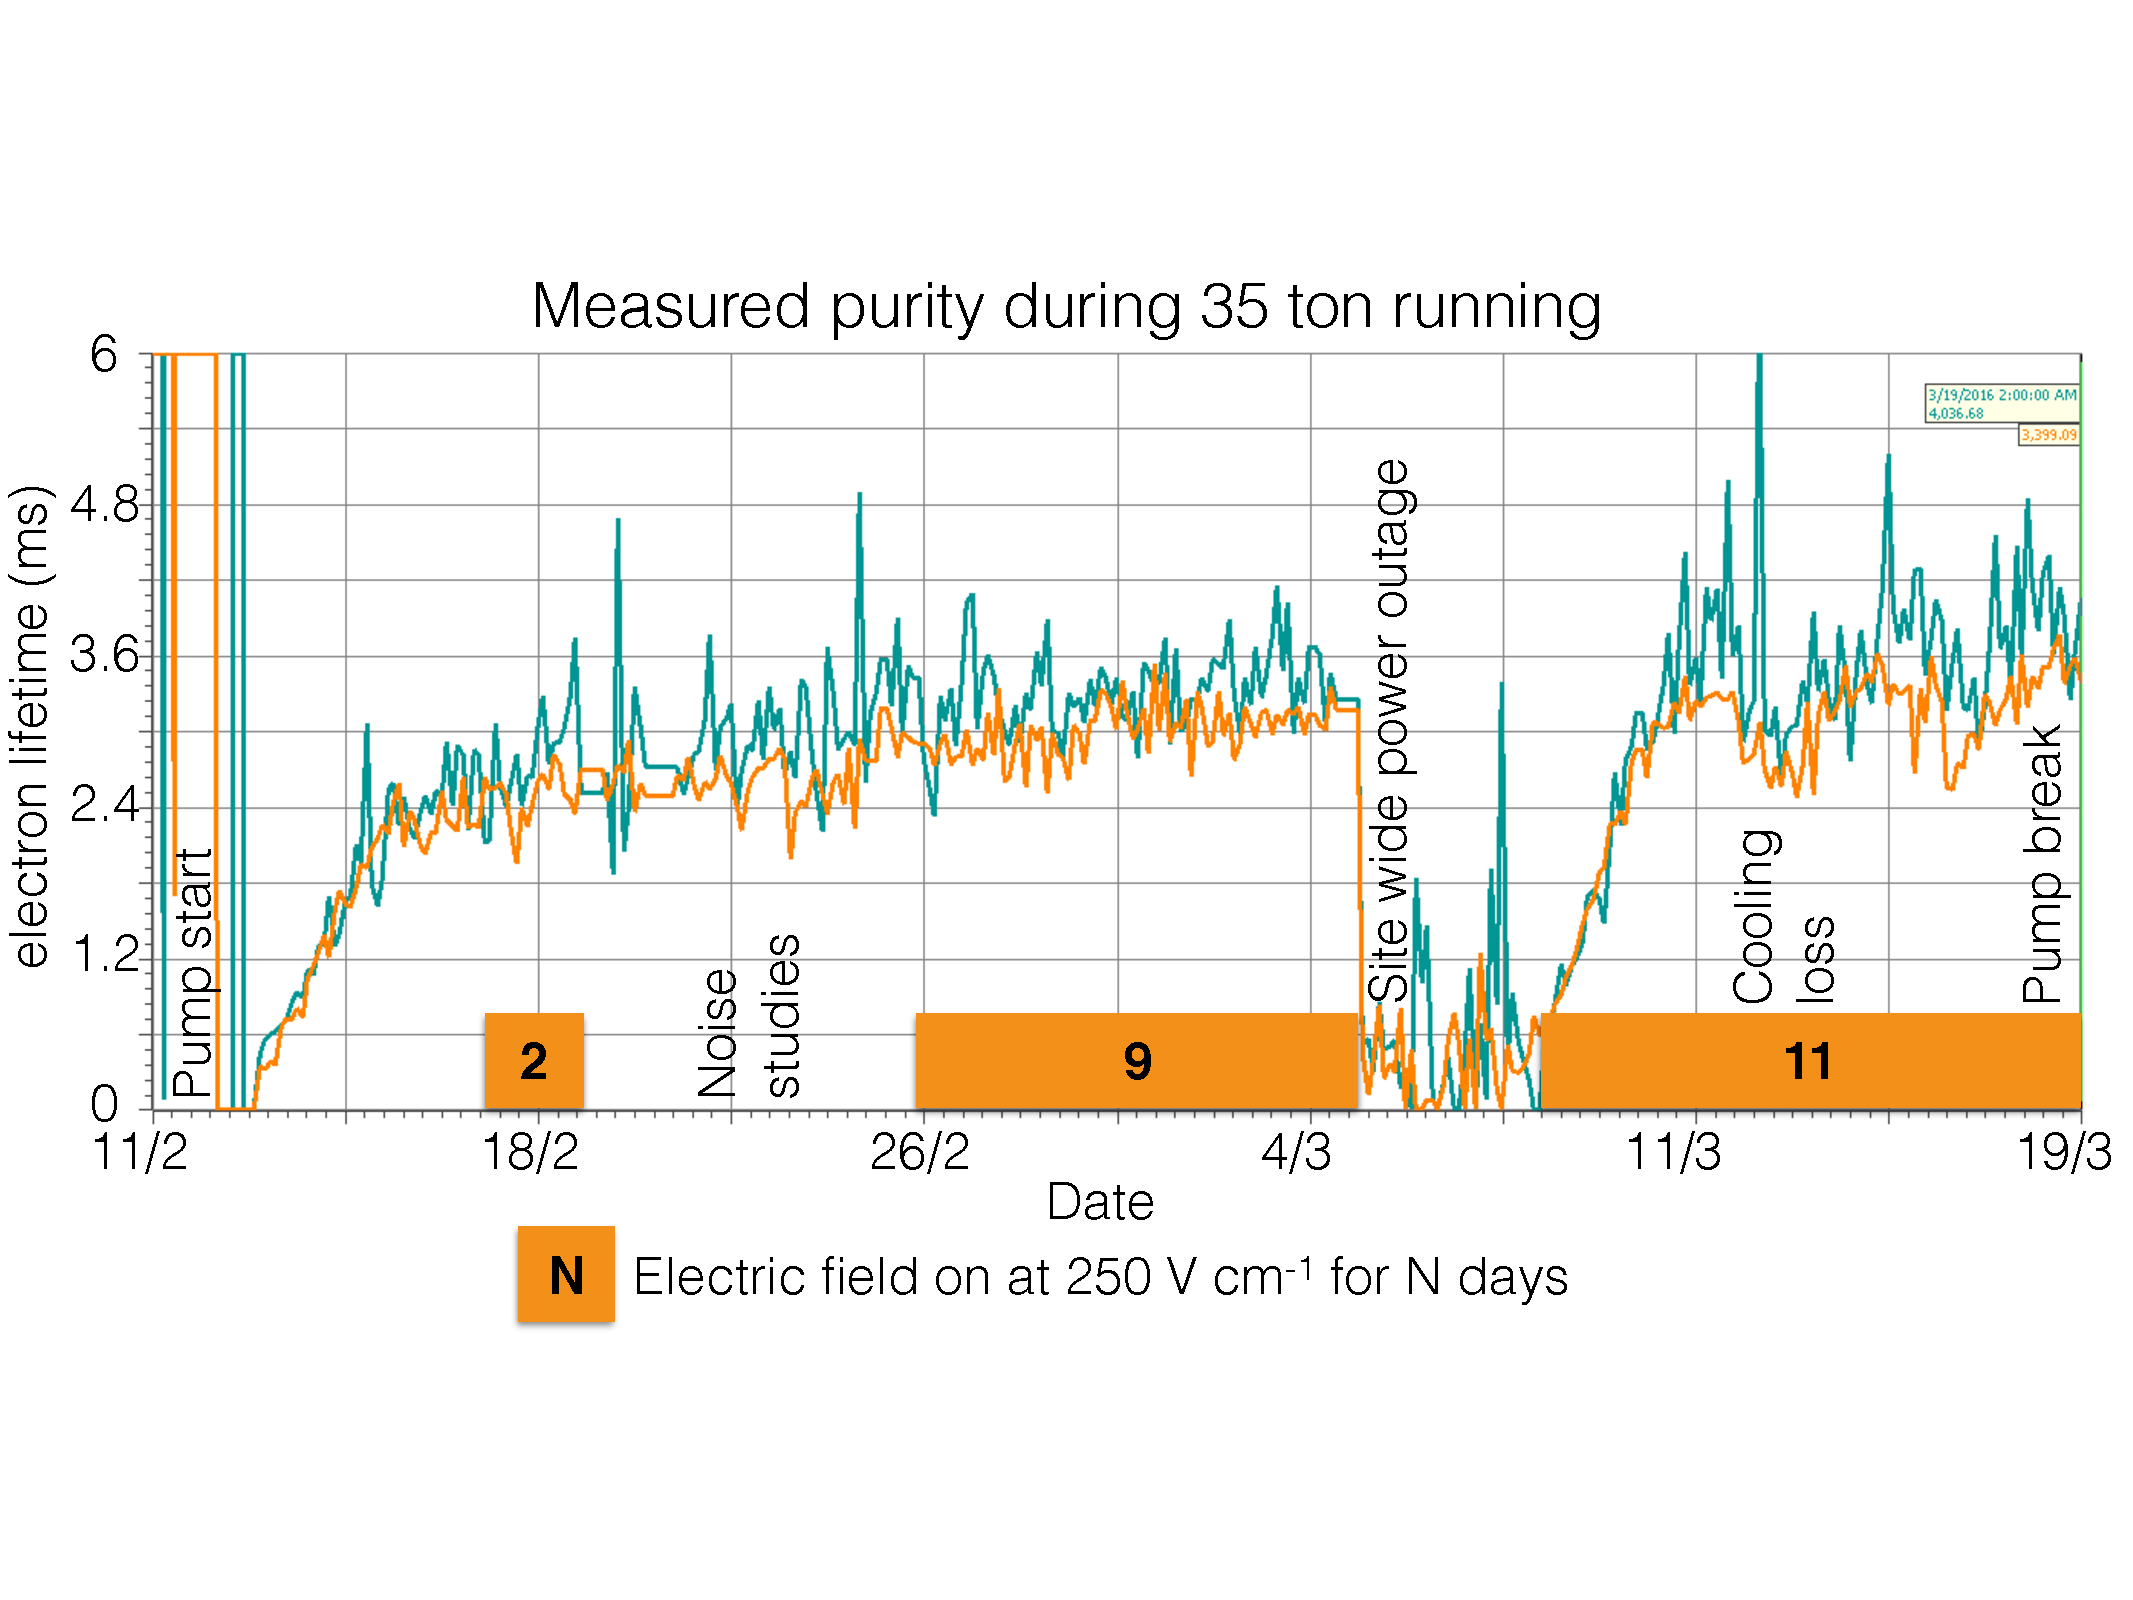
\includegraphics[width=1.0\textwidth]{DataCollected}
  \caption[The 35 ton data sample]{Timeline showing the data collected during the 35 ton Phase II run once the purification pumps were turned on.}
  \label{fig:DataCollected}  
\end{figure}

%********************************** %First Section  **************************************
\section{Organisation of the data structure} \label{Organisation of the data structure} %Section - X.1
The 35 ton detector consisted of three detector sub-systems: Reconfigurable Computing Elements (RCEs) collecting Time Projection Chamber (TPC) data, SiPM Signal Processors (SSPs) collecting photon detector data, and Cosmic Ray Counters (CRCs) tagging cosmic rays. The DAQ combined these three data streams into synchronous events in time and saved them as LArSoft data objects. These data objects would later have to be converted to the offline data products, which the reconstruction tools developed on simulation used, this is discussed in Section~\ref{Reformatting the data to the offline structure}. This section describes the structure of the data objects in the raw form.\\

During operations the DAQ was configured to maximise data throughput, and physics potential. This meant recording different lengths of times for each of the three sub-systems, as the data volumes and length of physics information were significantly different. For example, due to the emission of prompt light, the physics information from the SSPs is of a much shorter length of time than the physics information from the RCEs, where data has to be recorded whilst the electrons drift through the LAr. During the running period the recorded data was triggered by through-going muons which produced coincidences on the CRCs on opposites side of the cryostat. A coincidence is defined as two CRC modules recording a hit within 32 ns of each other. The system used to collect the CRC data was also responsible for generating the triggers, and so this meant that the trigger rate could be suppressed to approximately 1 Hz, by only producing triggers every N times a coincidence occurred, where N was a tuneable variable. A trigger rate of 1 Hz was used as the maximum speed at which data could be written to disk was approximately 60 MB$\cdot$s$^{-1}$, which is roughly equal to the size of each triggered event when the entire detector is read-out in the configuration discussed below. The rate at which events were recorded could have been increased if zero-suppression of the TPC data had been used, however the noise level meant that this was not feasible. \\ 

With an electric field of 250~V$\cdot$cm$^{-1}$, and a drift of 223~cm, the drift time for electrons at the long drift Cathode Plane Assembly (CPA) was roughly 2.6~ms or 5200~ticks (where 1~tick is 500 ns). It was decided that in order for a track causing a counter coincidence to be separated from other tracks in the detector, it was necessary to have roughly one drift window both before, and after, the drift window around the coincidence. This means that data was recorded for 7.5~ms, or 15,000~ticks, around each coincidence. The SSPs only collected the prompt light from through-going particles, and so only 200~$\mu$s of SSP data was recorded for each event. The CRCs produced the least volume of data, and so were able to be read out constantly. \\

As the run mode required accessing buffered data, it had to be discretised inside the components before being sent to the event builders in the DAQ. In the discussion of how this worked, focus will be given on the RCE data, where some new terms need to be introduced. The smallest unit of data, called a nanoslice, is the data from one RCE for one tick, where each RCE controls 128 channels. There were a total of 16 RCEs in the 35 ton detector, reading out 2048 channels. A microslice is then made by combining 1000$\times N$ nanoslices such that it contains 0.5~ms (1,000~ticks) of data across all channels, where $N$ is the number of RCEs that are recorded in the run. Microslices are then combined to make millislices, the length of which was configurable. Once produced, these millislices were sent by the DAQ to the event builders, to be stored as time synchronous LArSoft data objects. \\

The time synchronous events produced by the DAQ, did not, however, correspond to the physics events. This is because the DAQ was originally designed to produce a continuous data stream. This meant that the DAQ was configured to pad events with headers when a sub-system provided no physics information, such as nanoslices in the case of the RCEs. Removing these padded header objects was a remit of the online to offline converter discussed in Section~\ref{Reformatting the data to the offline structure}. The length of the millislices was configurable, and was chosen to be 10~ms (20,000~ticks) in order to best attempt to fully contain physics events, and reduce the need for the online to offline converter to stitch DAQ events together. The padding of millislices with headers between physics events introduced some peculiarities in the recorded data, such as millislices containing two parts of non-continuous data. This is shown in Figure~\ref{fig:DataStructure}, where the second millislice has no information for the time between the end of physics event 2 (2O), and the start of physics event 3 (2S).\\

\begin{figure}
  \centering
  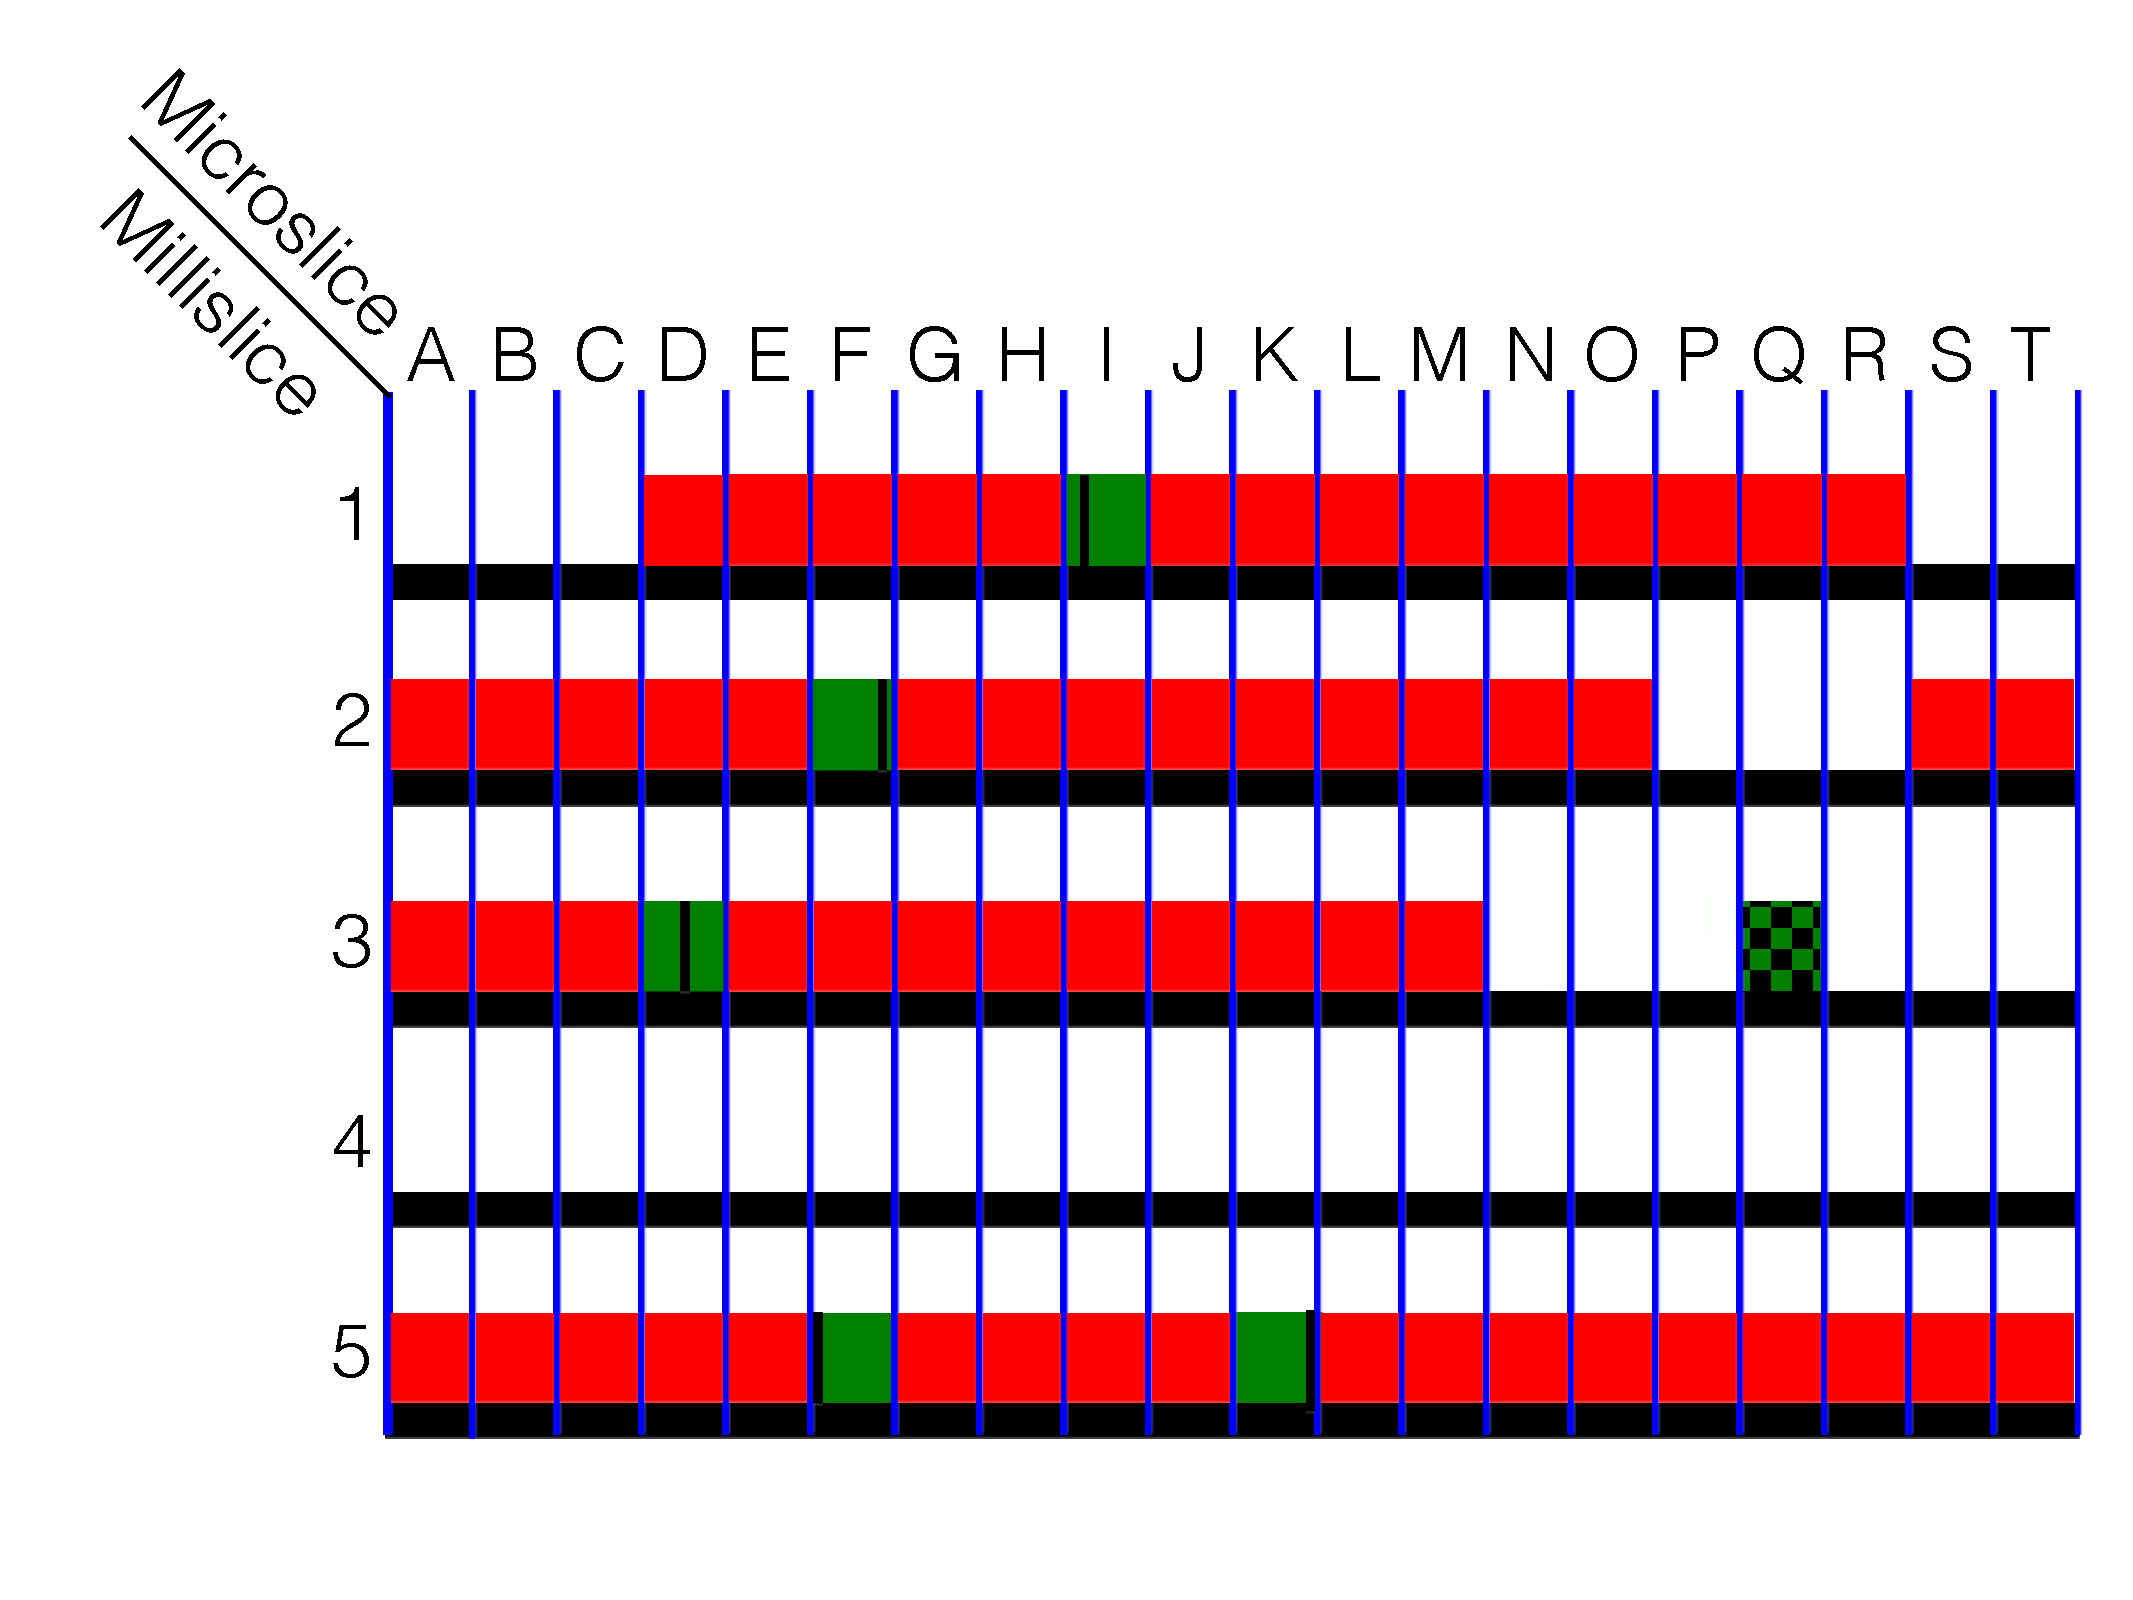
\includegraphics[width=0.75\textwidth]{DataStructure}
  \caption[The 35 ton data structure]
          {A diagram of possible millislice structures for the TPC data recorded by the 35 ton detector. Each row represents a millislice (numbered 1 to 5), whilst each box represents a microslice (labelled A to T). The vertical blue lines delineate each microslice, giving 20 microslices per millislice. Solid red and green boxes represent microslices with TPC data in them. A group of 15 continuous red and green boxes are the recorded ``physics events''. Green boxes represent triggers which were used, with the black lines showing the time in the millislice at which the trigger occurred. The green and black patterned box in microslice 3Q represents a coincidence which was not issued as a trigger. A possible reason for this trigger not being issued, is its proximity to a previous coincidence trigger which was issued from the same co-incidence.}
  \label{fig:DataStructure}
\end{figure}

During normal data taking microslices were buffered in the RCEs, so that if a trigger was issued they could be accessed before being deleted. As the data was buffered in the form of microslices, previous microslices could only be accessed as a whole. This meant that a whole number of microslices had to be loaded before the trigger, so when a trigger was issued part way through a microslice, the previous $X$ microslices were sent to the event builders, where $X$ was typically 5. As a result, there are always a minimum number of ticks both before (5,000~ticks) and after (9,000~ticks) the trigger, but the exact numbers can change by up to 1,000~ticks for a given event, depending on where in the microslice the trigger came. The result of this is that it is impossible to know the number of ticks before/after a given counter coincidence. This is shown in Figure~\ref{fig:DataStructure} where the black lines representing triggers, are seen to occur at different points within the microslices. For example, physics event 1 (1D to 1R) will have more data after the trigger than physics event 2 (2A to 2O), as the trigger occurred earlier in the triggered microslice.

%********************************** %Second Section  *************************************
\section{Reformatting the data to the offline structure} \label{Reformatting the data to the offline structure} %Section - X.2
Conversion of the data objects stored in the raw data to the data objects used in simulation required a suite of unpacking services to be written, the specifics of which are not discussed here. These all required a common interface through which to access the data, and check that the timing of each component was consistent, so that a final LArSoft file for downstream use could be produced. This interface had the added role of producing complete physics events, meaning that it had to be able to combine multiple millislices, and extract only the data containing the continuous physics events. \\

Following the unpacking of each of the sub-systems, the data reformatter would loop through the TPC ticks to see if a user defined set of conditions could be satisfied at that time. These conditions were usually whether an east-west or north-south counter coincidence (see Figure~\ref{fig:35tonCounterLoc}) occurred at that time, or if this millislice contained TPC data whilst the previous one did not. The latter was the default configuration, as this gave the option of preserving all of the data gathered, for reasons discussed at the end of Section~\ref{Organisation of the data structure}. Other conditions were available, though rarely used, such as if the SSPs observed a large flash of flight, or if there was a large change in the average TPC Analogue-to-Digital Converter (ADC) value. Once a set of conditions are satisfied, a user defined number of pre-condition ticks are gathered. No pre-condition ticks are gathered when the previous millislice contains no TPC data, as there is no previous data to load which would not have a gap in time, see Figure~\ref{fig:DataStructure}, millislice 5. In the case of using a counter coincidence to make an event, a value of 300 pre-condition ticks is normally used, with a maximum of 5000~ticks being able to reliably collected. Once the pre-condition ticks are gathered, a further $N$ post-condition ticks are gathered, where $N$ is defined by the user. Usually 15,000~ticks are gathered when the previous millislice is empty, and 5,200~ticks are gathered when there is a coincidence, though a maximum of 9,000~ticks could be reliably gathered. Data from the other components is added to the event if its timestamp is within the timestamps of the first and last ticks in the event. This is done either, when no more TPC data is required, or at the end of a millislice if stitching is required. All timestamps are corrected such that the event began at $t$ = 0, as the reconstruction assumes this, and the timestamp of the start of the event is stored in the event record so that it can be accessed later if required. \\

It is important to integrate flexibility at all points in this process, so that the user can choose the length of events, which sub-systems are in the events, and what the conditions are for making events. It is also important for users to be able to run the service on already formatted events, as the unpacking services are the major overhead in running the interface. It is also conceivable that users would want to reformat Monte Carlo events so as to centre them around their chosen conditions, and so the use of the unpacking algorithms was determined by the interface depending on the format of the input file.

%********************************** % Third Section  *************************************
\section{Observations on data quality and noise mitigation} \label{sec:AllTheNoise} %Section - X.3
Reformatting the online data to the offline format was an important step in maintaining data quality, as subsequently there was no access to the raw data due to the framework of the 35 ton software. Some of the important checks which are performed are outlined in Figure~\ref{fig:DataDrops}. If any of these issues are present in a given physics event it is discarded as the integrity of the data cannot be guaranteed. It was decided that these events would be discarded as non-synchronous events would lead to hits in the detector being at incorrect times, and padding empty events with pedestals could mean that tracks seem to disappear as they travel through the detector, only to reappear at a later time in a different detector location. \\

Another example of an inconsistent event is when the sub-systems are not synchronised with each other. This is normally caused by one of the sub-systems missing a clock increment from the master timing unit, due to the data trigger being issued close to an increment from the master unit. This misalignment causes an incorrect time sample being read out, and so the data from each sub-system within a millislice is not consistent. The result of this is that the event will fail the timestamp check, and so won't be added to the event record. To avoid incomplete events, these physics events are also discarded when observed. \\

\begin{figure}
  \centering
  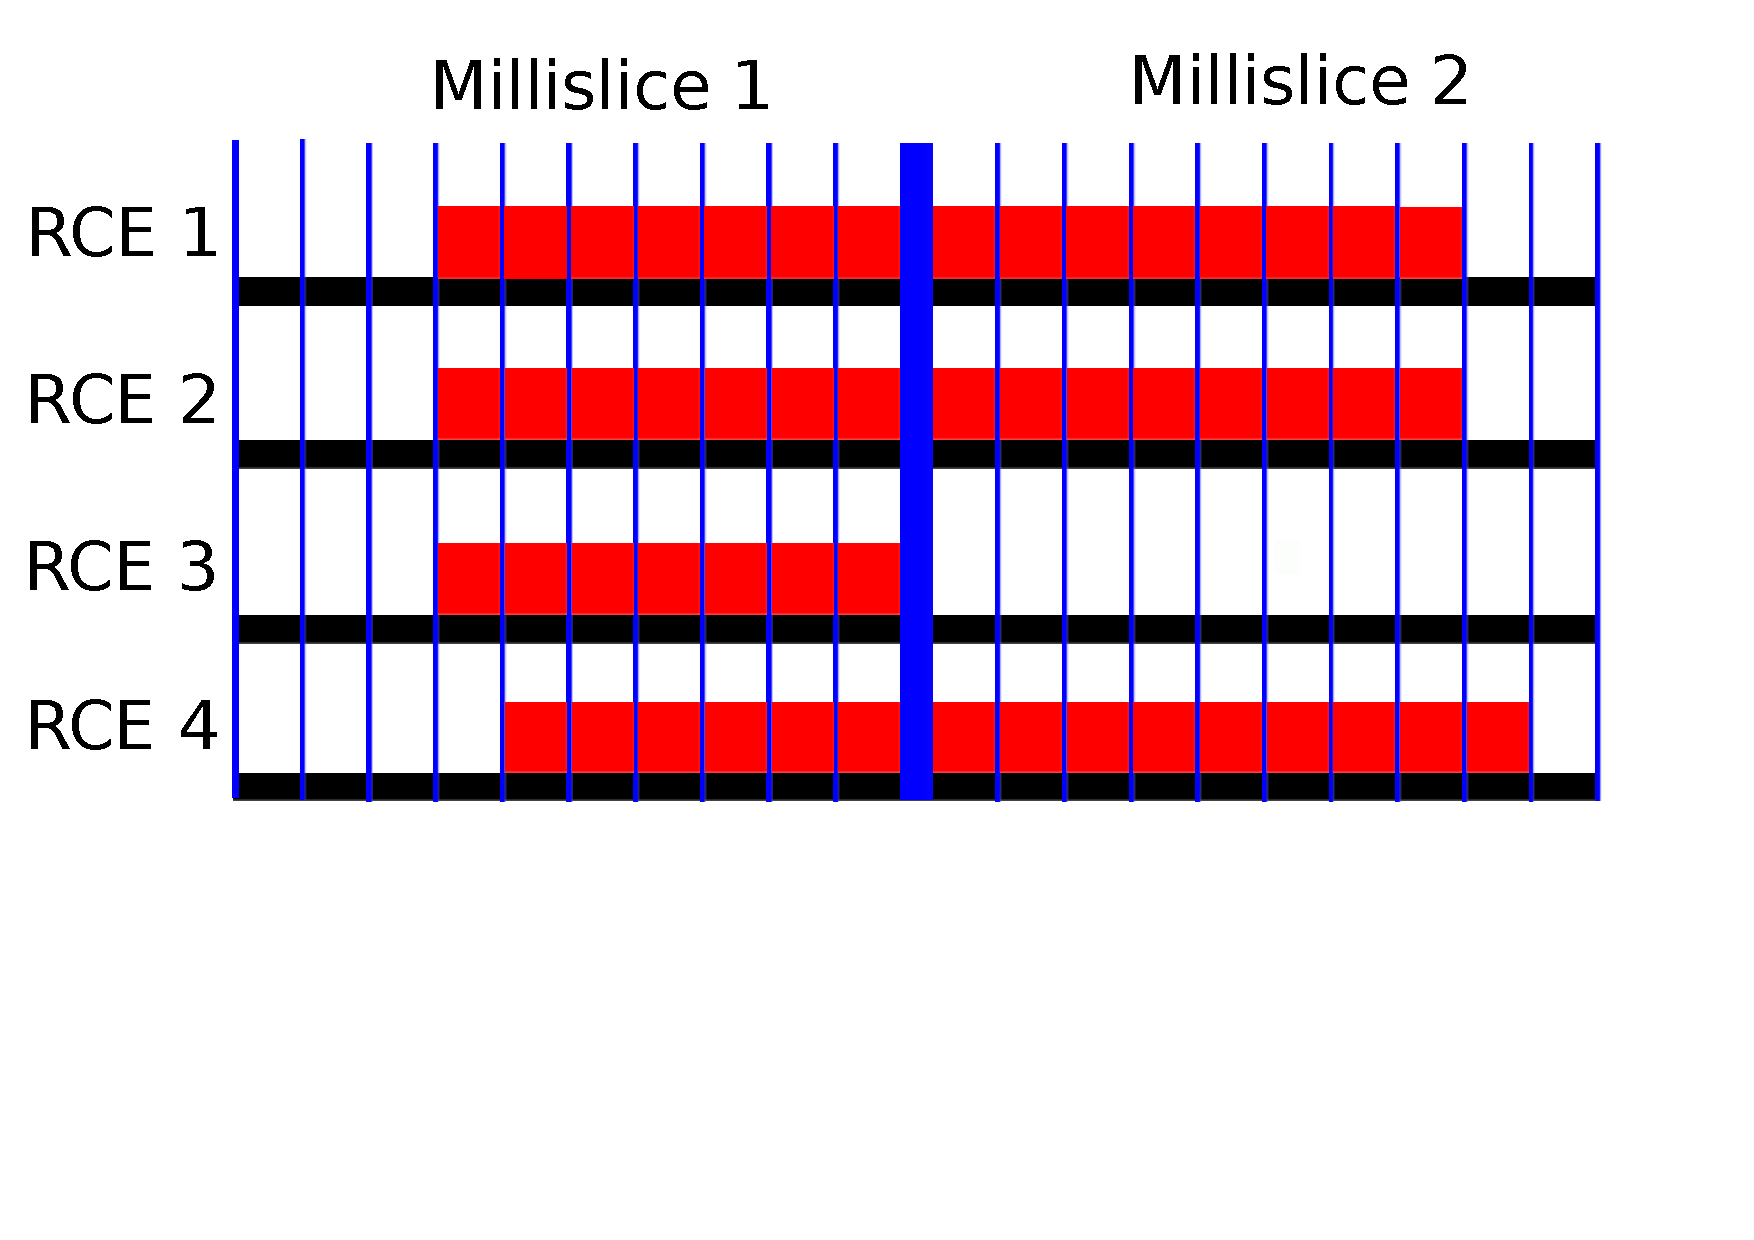
\includegraphics[width=0.85\textwidth]{DataDrops}
  \caption[Dropped TPC data in the 35 ton]
          {A diagram of TPC microslices within millislices in the 35 ton data stream. Two millislices are shown, each containing 10 microslices. One physics event straddling the millislice boundaries is shown, and 4 RCEs representing each row are read out. The vertical blue lines delineate each microslice (0.5~ms, 1,000~ticks), with the thick blue line showing the millislice boundary. Solid red boxes represent microslices with TPC data in them. It can be seen that RCEs 1 and 2 contain data for the same interval, whilst the data from RCE 3 in millislice 2 has been ``Dropped,'' and the data from RCE 4 is shifted by 1 microslice from RCEs 1 and 2 and is thus ``Inconsistent.'' As a result of these issues this physics event would be discarded, as data integrity cannot be guaranteed.}
  \label{fig:DataDrops}
\end{figure}

The electronic noise in the 35 ton was higher than anticipated, with the RMS of the RCE ADC being approximately 30 counts, compared to an expected thermal noise of around 2.5~ADC counts. Many sources contributed to this elevated noise, some of which are explained below. \\

Though not directly affecting the noise issues ``stuck ADC codes'' were a feature of the data which had to removed. ``Stuck ADC codes'' were caused by bit level corruption where the lowest 6 bits in the ADC became frozen to either {\tt 0x0} or {\tt 0x3f}. This was observed during the first stages of commissioning, and an algorithm to remove them was developed and tested on Monte Carlo~\citep{InslerStuckCode}. In simulations it was observed that the signal could be recovered with minimal losses, as shown in Figure~\ref{fig:StuckCodes}, where the signals after stuck code removal (blue lines) are seen to closely match the signals before stuck codes were added (black lines). \\

\begin{figure}
  \centering
  \begin{subfigure}{0.48\textwidth}
    \centering
    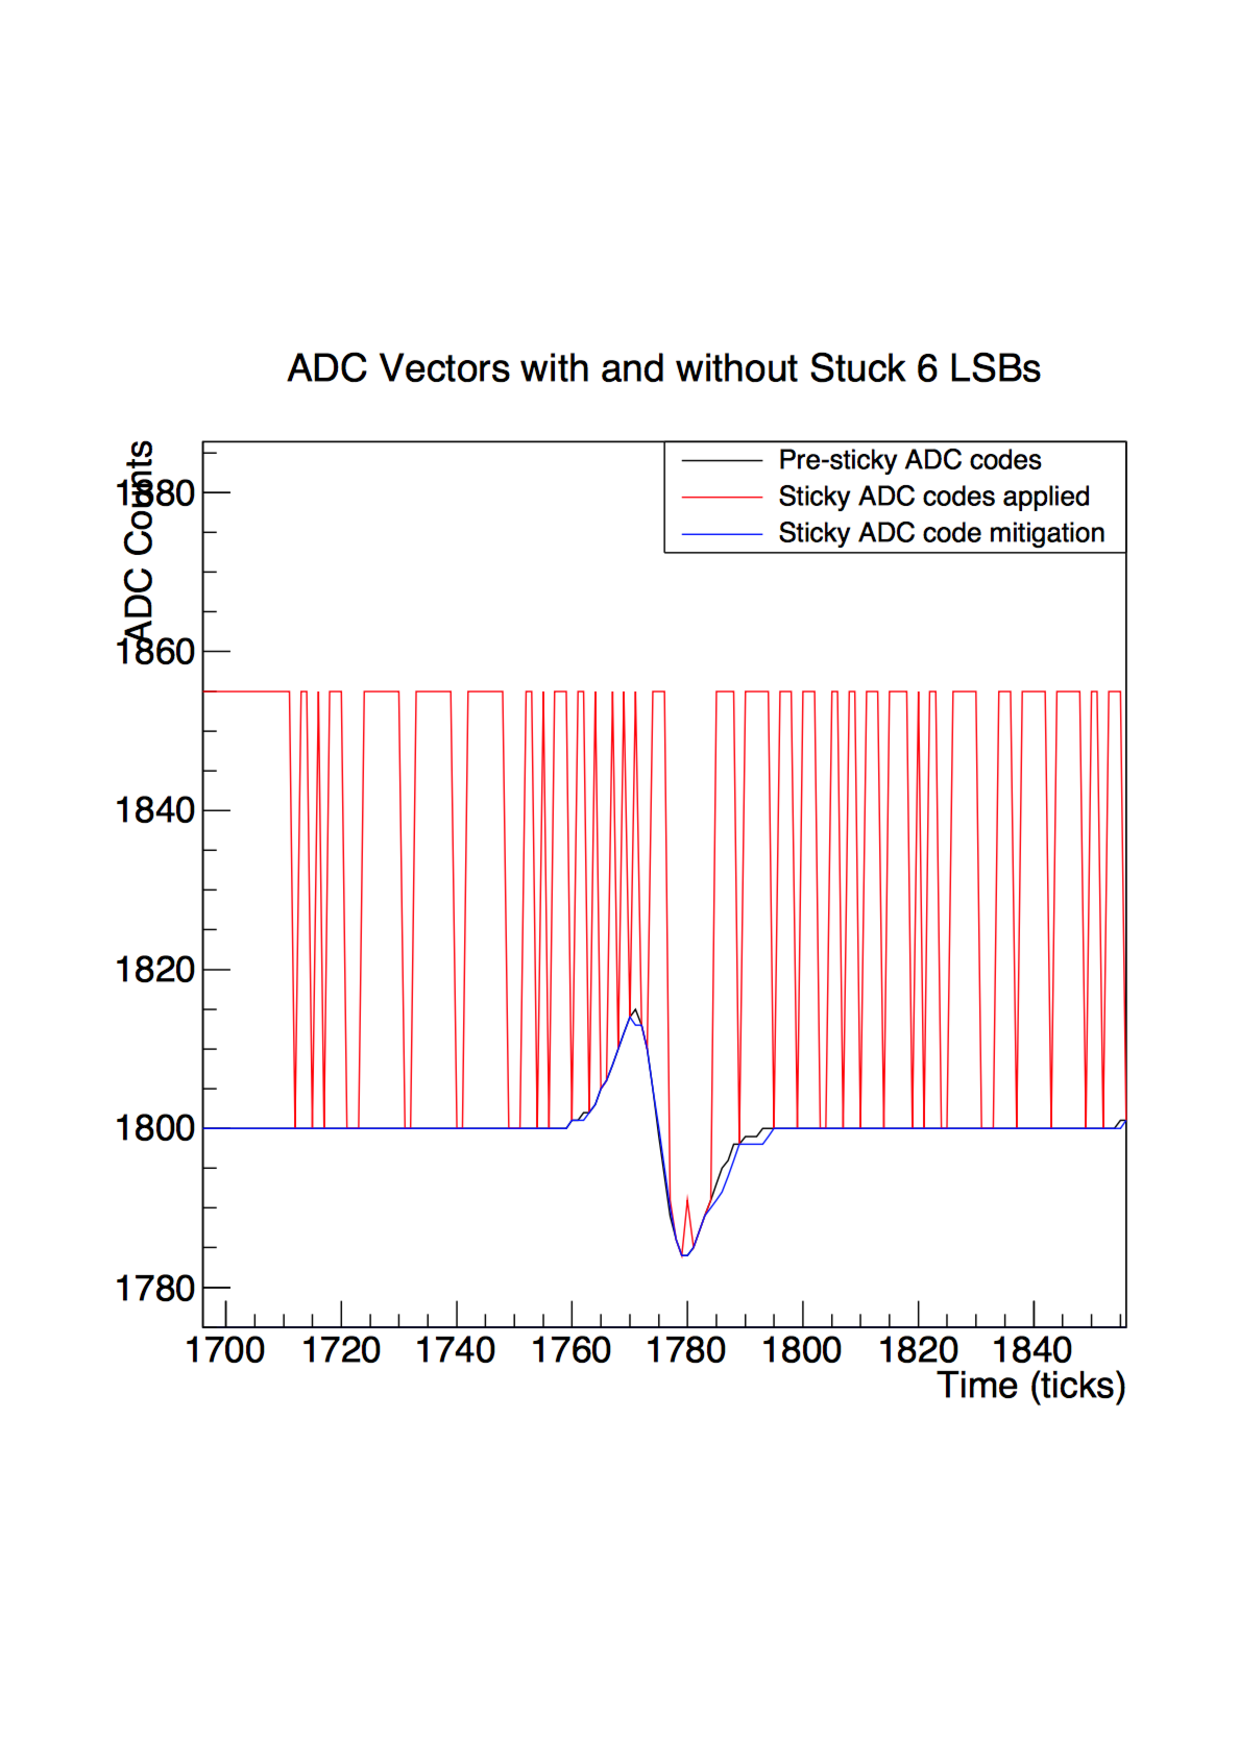
\includegraphics[width=\textwidth]{StuckCodes}
  \end{subfigure}%
  \hspace{0.03\textwidth}%
  \begin{subfigure}{0.48\textwidth}
    \centering
    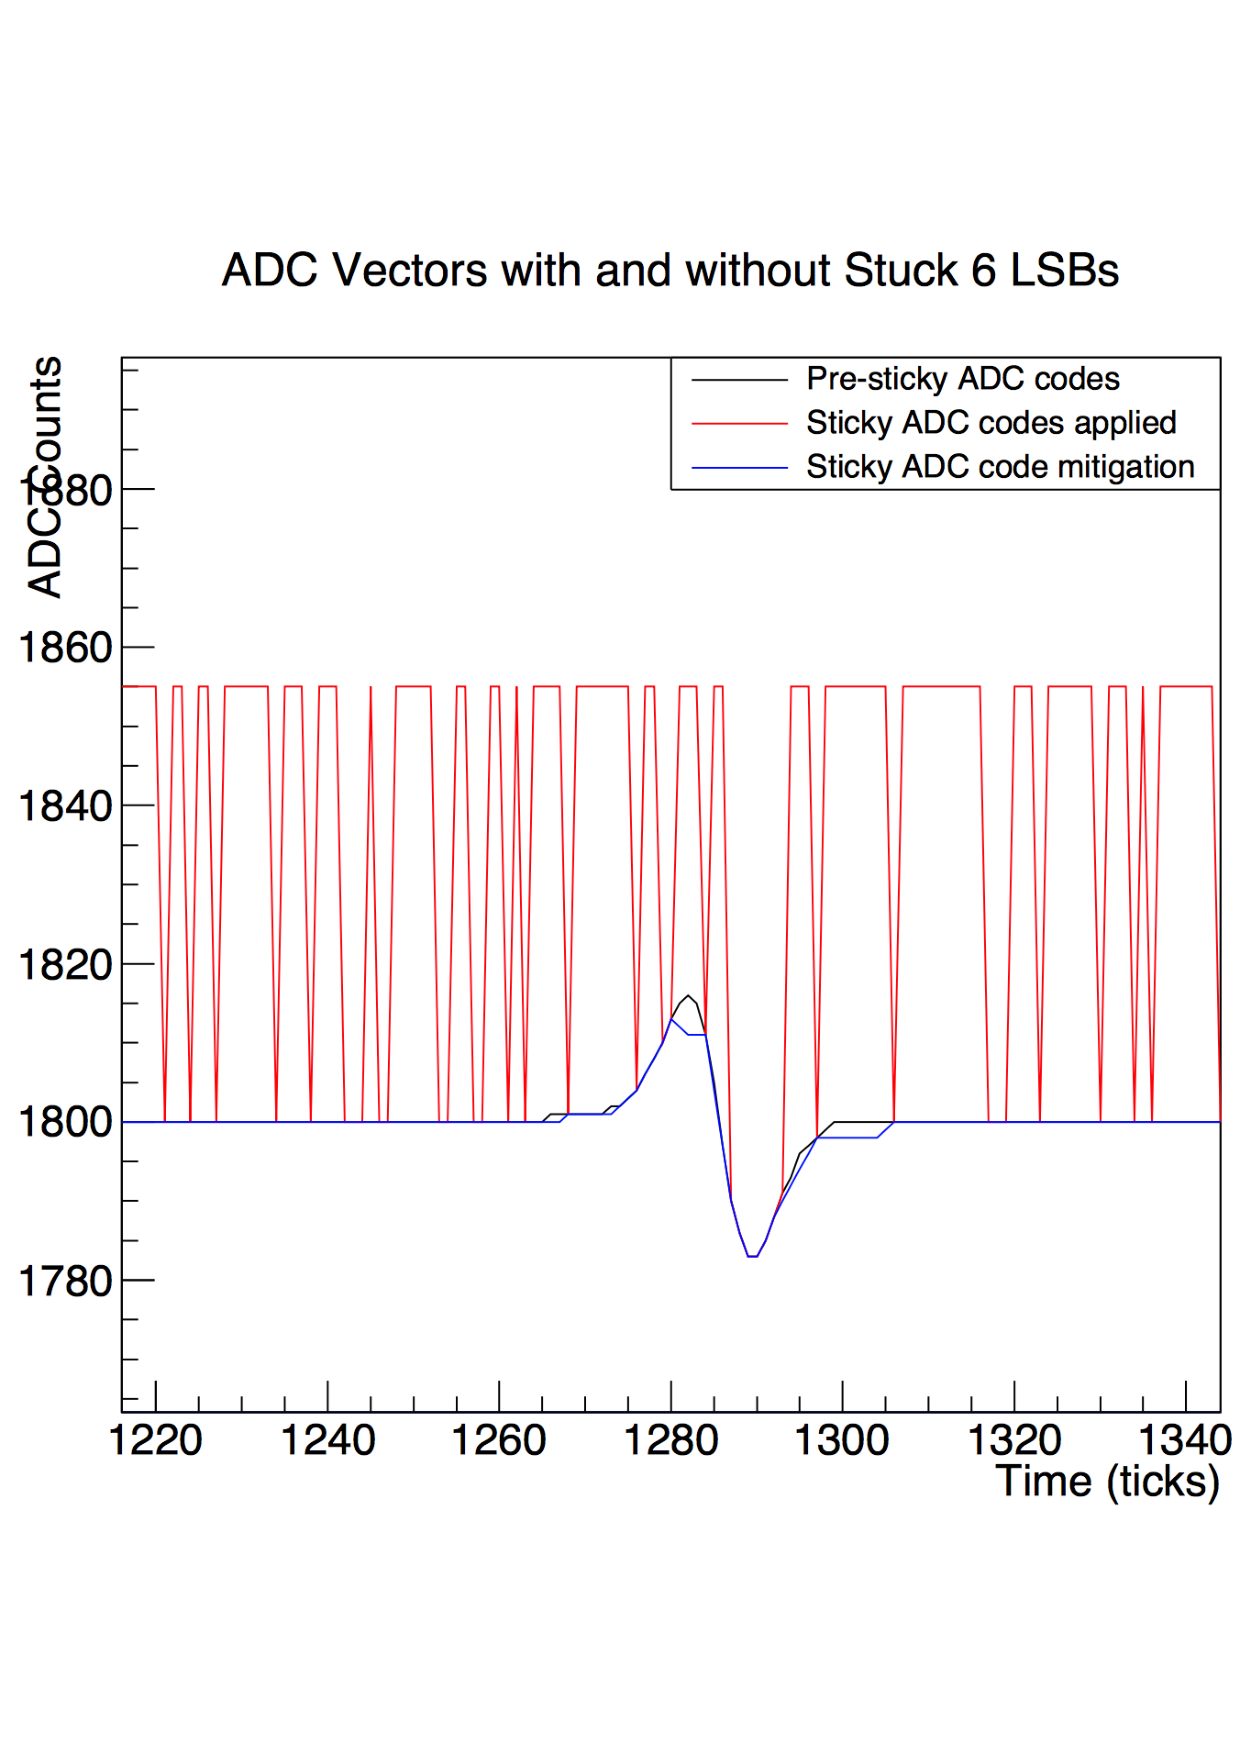
\includegraphics[width=\textwidth]{StuckCodes2}
  \end{subfigure}
  \caption[Recovering stuck ADC codes in the 35 ton]
          {Two Monte Carlo spectra showing the effect of the introduction and removal of stuck bits on a simulated signal. The black line shows the simulated signal on a wire, which is then modified by adding the effects of ``stuck ADC codes,'' shown by the red line. The ``stuck ADC codes'' are then removed, and the resulting signal is given by the blue line. It can be seen that the signal loss is minimal after the ``stuck ADC codes'' are removed. The figures were taken from~\citep{InslerStuckCode}.}
          \label{fig:StuckCodes}
\end{figure}

A significant portion of the noise was correlated between groups of 32 channels, where the ADCs would coherently oscillate. To remove these coherent shifts, ADC baselines were calculated for these groups of 32 channels at each tick, and then subtracted from the measured ADC values. This was found to be an effective method of removing coherent noise in MicroBooNE~\citep{uBooNENoise}. The effect of removing coherent noise is shown in Figure~\ref{fig:CoherentNoise}, where the signal peak becomes much easier to discern after noise removal, and a coherent noise peak around tick 6030 is removed. An issue with removing coherent noise in this way is that events which are parallel to the Anode Plane Assembly (APA) frames will produce signals at common times, and across adjacent wires, and these signals may be removed along with the coherent noise. This will cause a reduction in the hit reconstruction efficiency. The only way to prevent this is to ``protect'' potential signal regions from the coherent noise removal, as is done in MicroBooNE~\citep{uBooNENoise}. \\

\begin{figure}
  \centering
  \begin{subfigure}{0.48\textwidth}
    \centering
    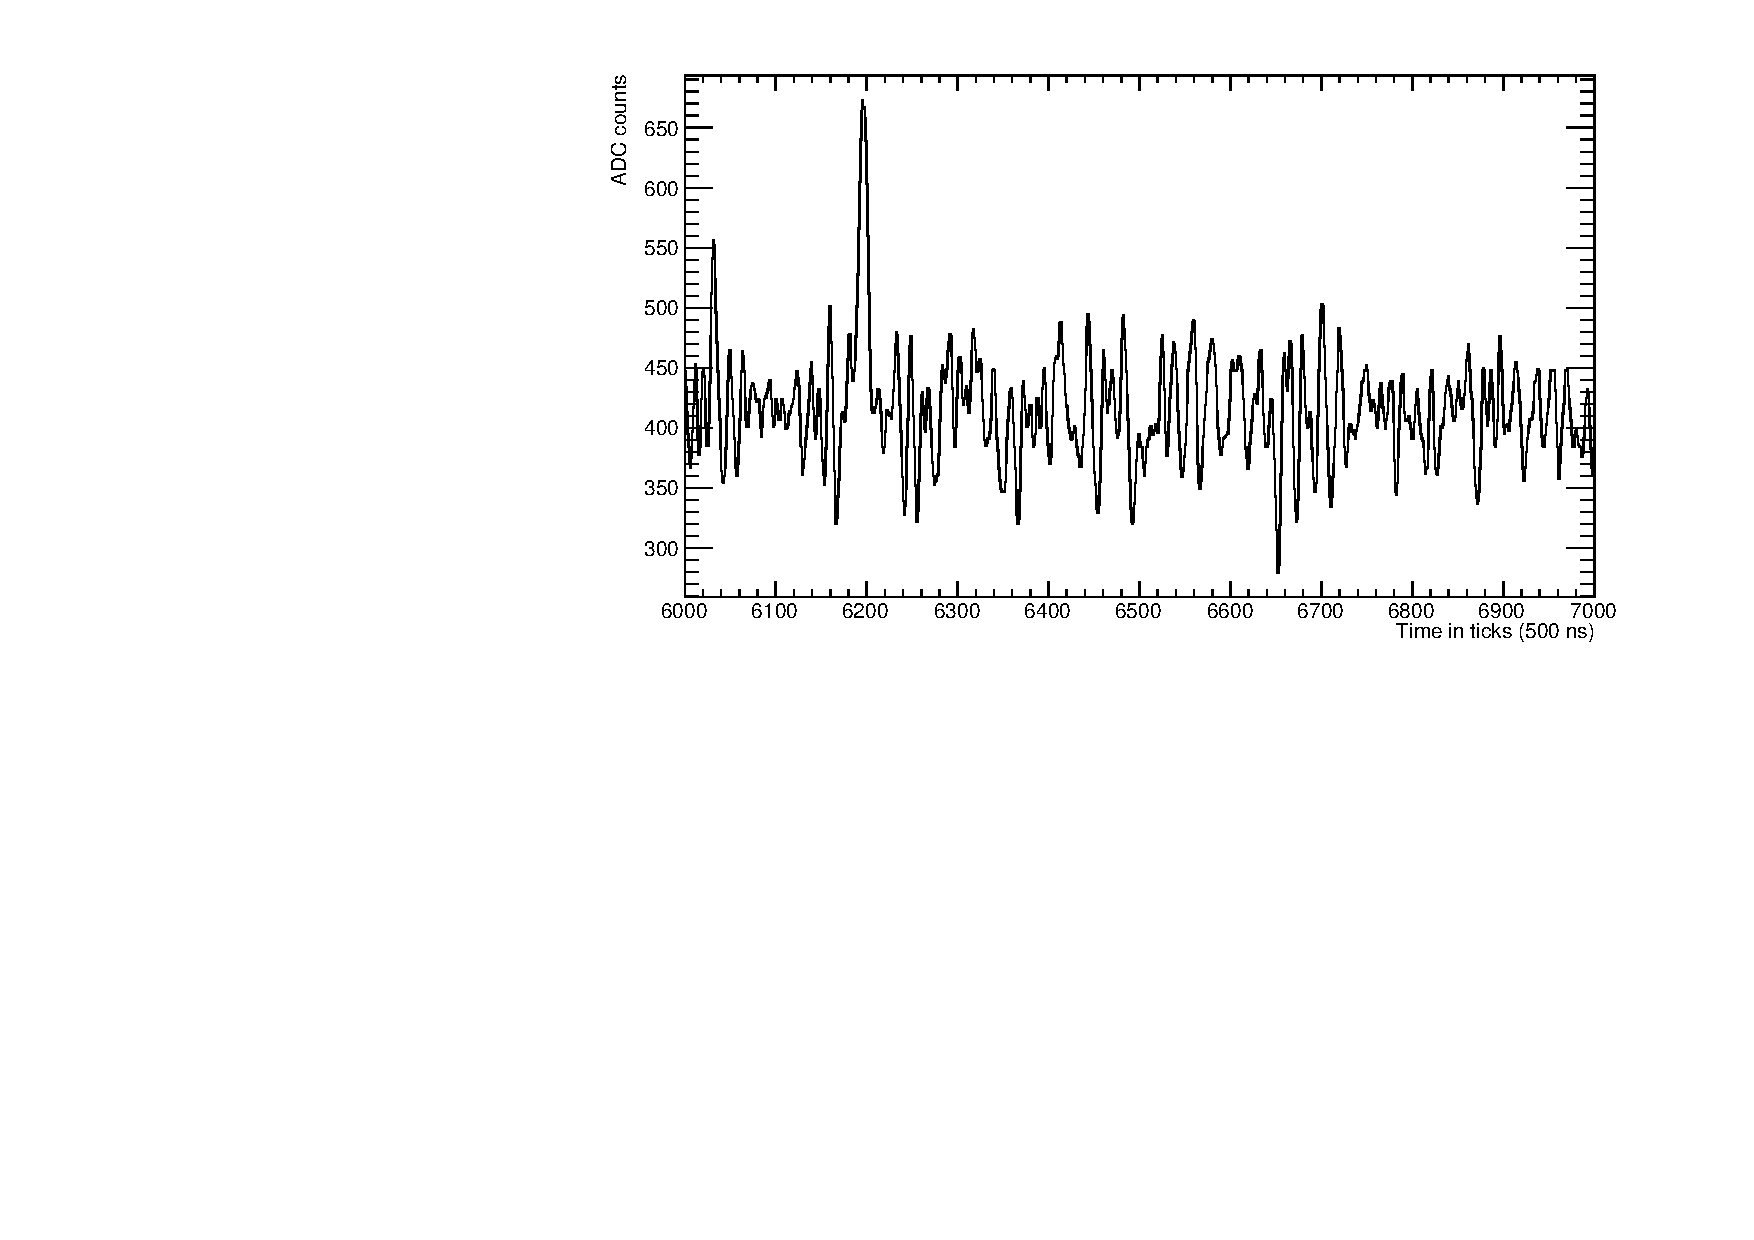
\includegraphics[width=\textwidth]{BeforeCoherent}
    \caption{Before coherent noise removal}
  \end{subfigure}%
  \hspace{0.03\textwidth}%
  \begin{subfigure}{0.48\textwidth}
    \centering
    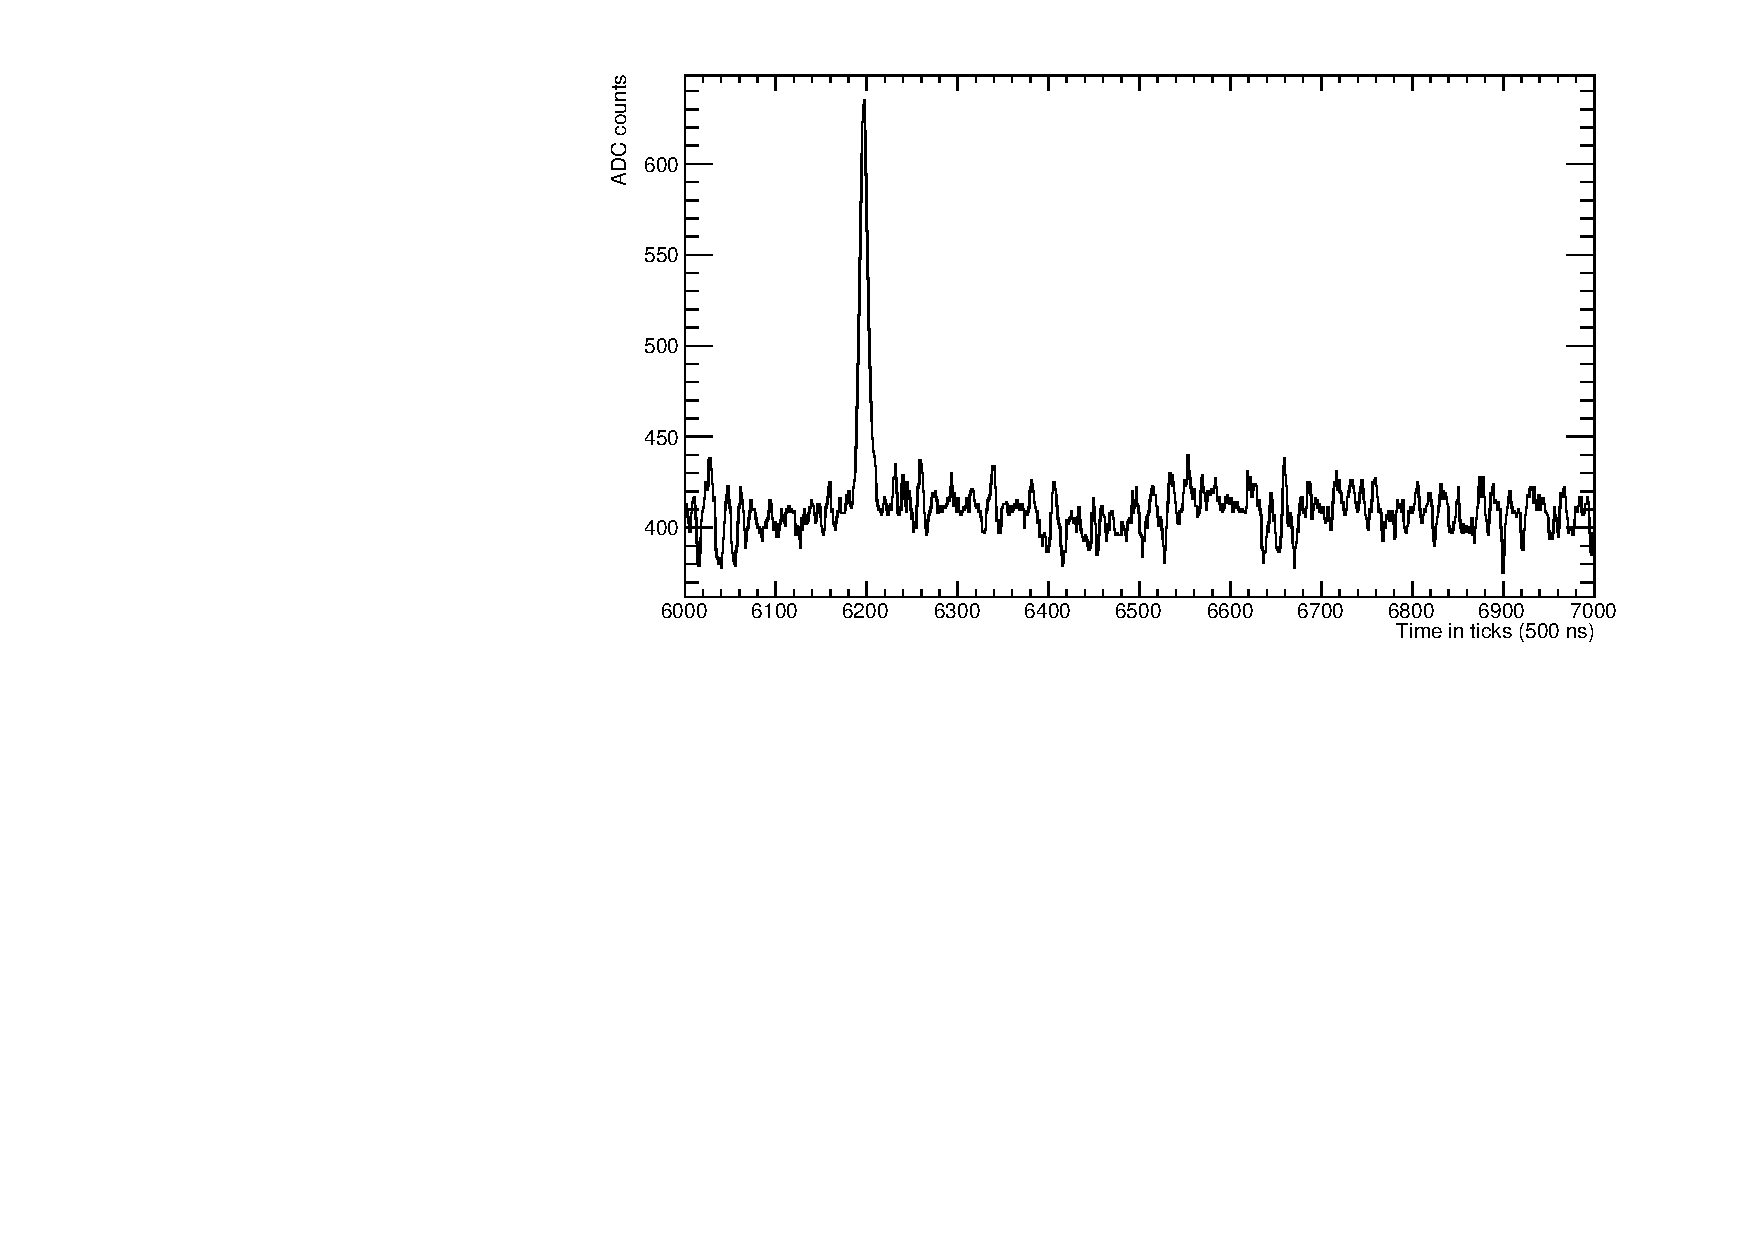
\includegraphics[width=\textwidth]{AfterCoherent}
    \caption{After coherent noise removal}
  \end{subfigure}
  \caption[Removing coherent noise in the 35 ton]
          {The effect of coherent noise removal on a 35 ton signal event. Left: the signal before coherent noise is removed. Right: the signal after the coherent is removed. The signal peak around tick 6200 is much clearer after coherent noise removal, meaning that hit reconstruction becomes much simpler.}
  \label{fig:CoherentNoise}
\end{figure}

After performing a Fast Fourier Transform (FFT)~\citep{CoTuFFT} on the coherent noise subtracted waveforms, it can be seen that signals occur with specific frequencies. Some of these frequencies are caused by real energy depositions, whilst others are due to the electronics noise. It is possible to remove the noise frequencies by applying Wiener filters~\citep{WienerFilter}. Frequency spectra are taken for each of the three planes, and a clear signal is both preserved and suppressed. The raw signal spectra are then divided by the signal suppressed spectra, to produce $signal/noise$ frequency spaces. The regions of frequency space to be conserved, given by regions of high $signal/noise$, can then be found by fitting a combination of sigmoid functions to the frequency spaces. Equations~\ref{eq:SigCol},~and~\ref{eq:SigInd} show the sigmoid functions which are applied to the collection and induction planes respectively.  
\begin{align}
  f(x)_{Col} &= 1 - \frac{1}{1 + exp( -(x - A_{Col})/B_{Col} ) } \label{eq:SigCol} \\
  f(x)_{Ind} &= \left[ 1 - \frac{1}{1 + exp( -(x - A_{Ind})/B_{Ind} ) } \right] \times \left[ \frac{1}{1 + exp( -(x - C_{Ind})/D_{Ind} ) } \right] \label{eq:SigInd}
\end{align}
where $A_{Col}$, $B_{Col}$, $A_{Ind}$, $B_{Ind}$, $C_{Ind}$ and $D_{Ind}$ are tuned for each plane. A demonstration of how this was applied is shown in Figure~\ref{fig:FrequencyFilter}. It is also possible to remove specific frequencies which are not removed by the filters, this was necessary for a 54 KHz noise component which was introduced by the fluorescent lights in the detector hall. After the run ended it was found that some of the high frequency noise components were introduced by a short on a warm power cable. The techniques used to find this cable will be used when commissioning future detectors~\citep{35tonNoiseMeeting}. \\

\begin{figure}
  \centering
  \begin{subfigure}{0.48\textwidth}
    \centering
    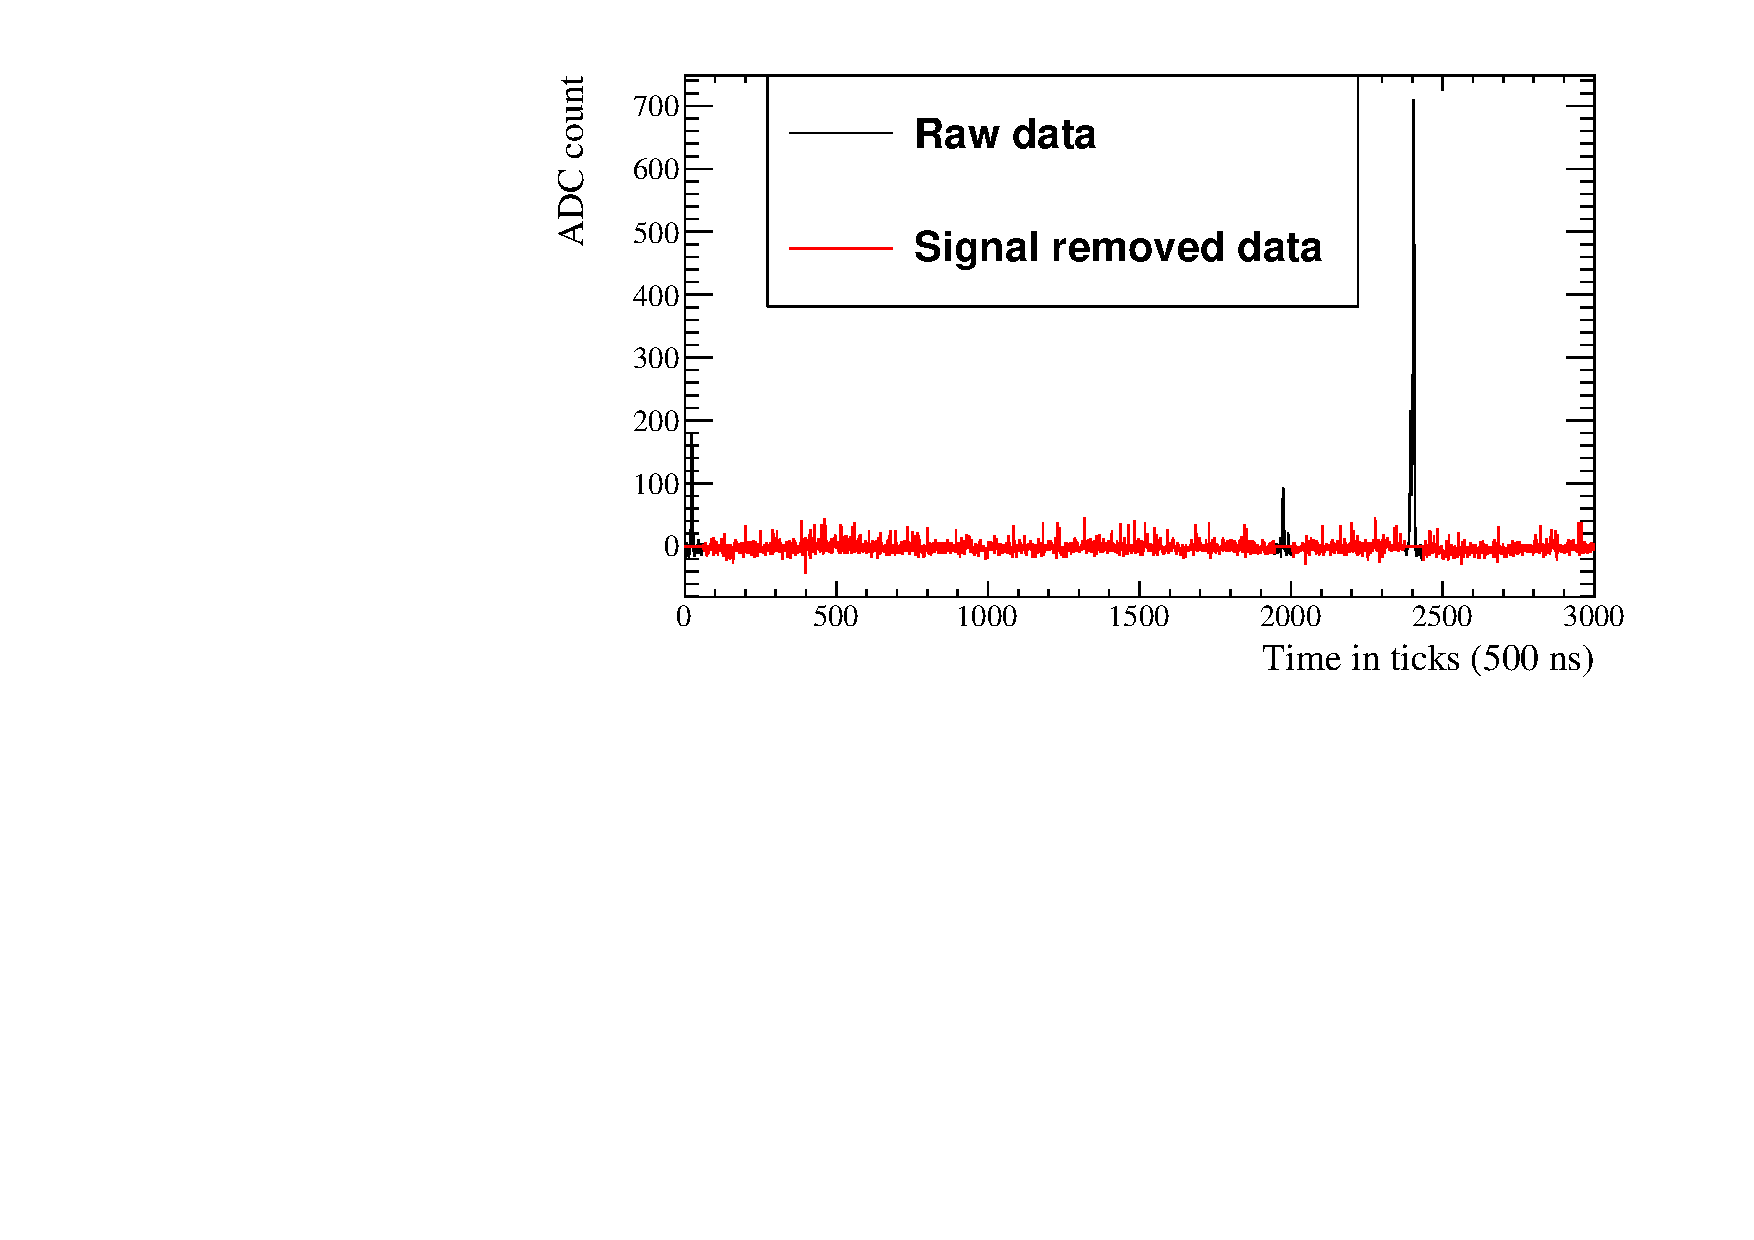
\includegraphics[width=\textwidth]{Waveforms}
    \caption{A raw and signal subtracted waveform for a collection plane wire.}
    \label{fig:FreqWaveform}
  \end{subfigure}%
  \hspace{0.03\textwidth}%
  \begin{subfigure}{0.48\textwidth}
    \centering
    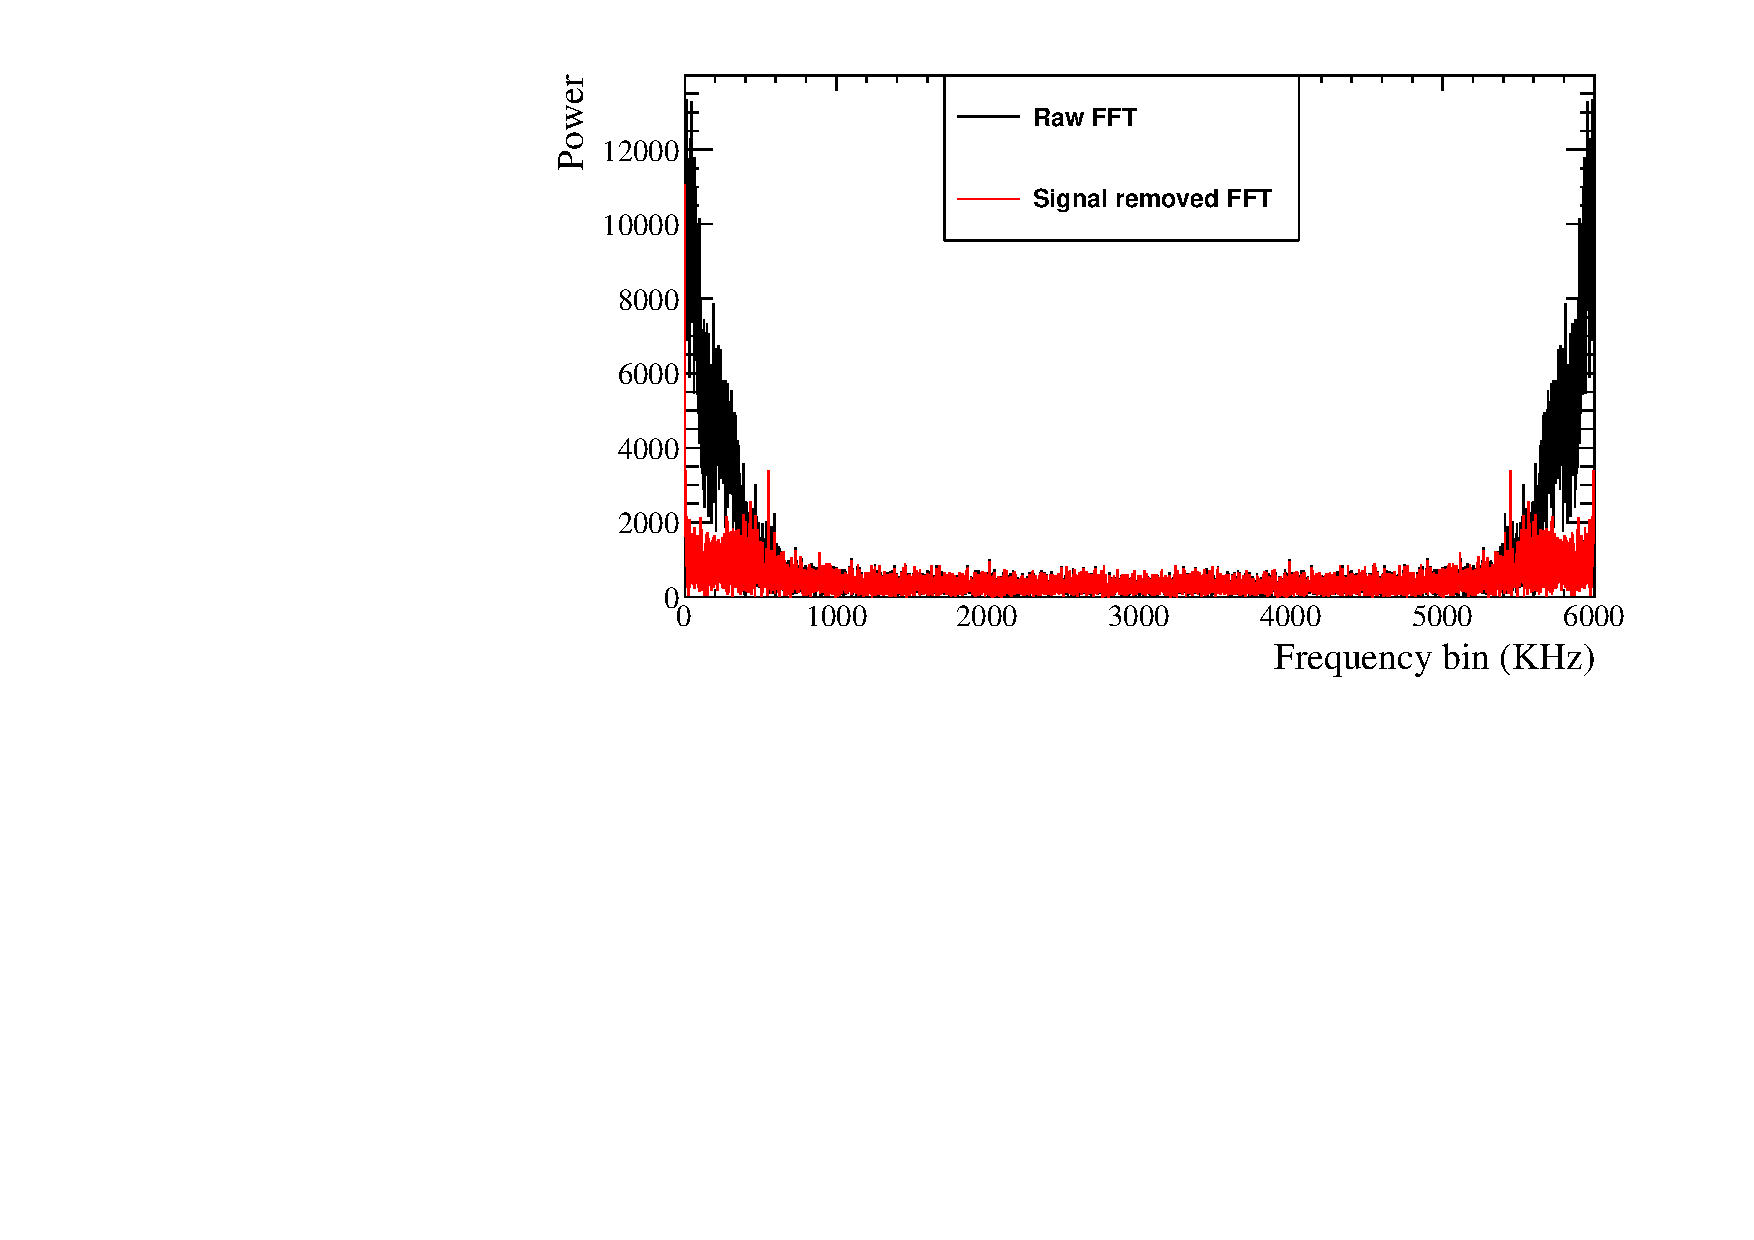
\includegraphics[width=\textwidth]{NoiseFFTs}
    \caption{The FFT of the raw and signal subtracted waveform for a collection plane wire.}
    \label{fig:FreqFFT}
  \end{subfigure}
  \begin{subfigure}{0.48\textwidth}
    \centering
    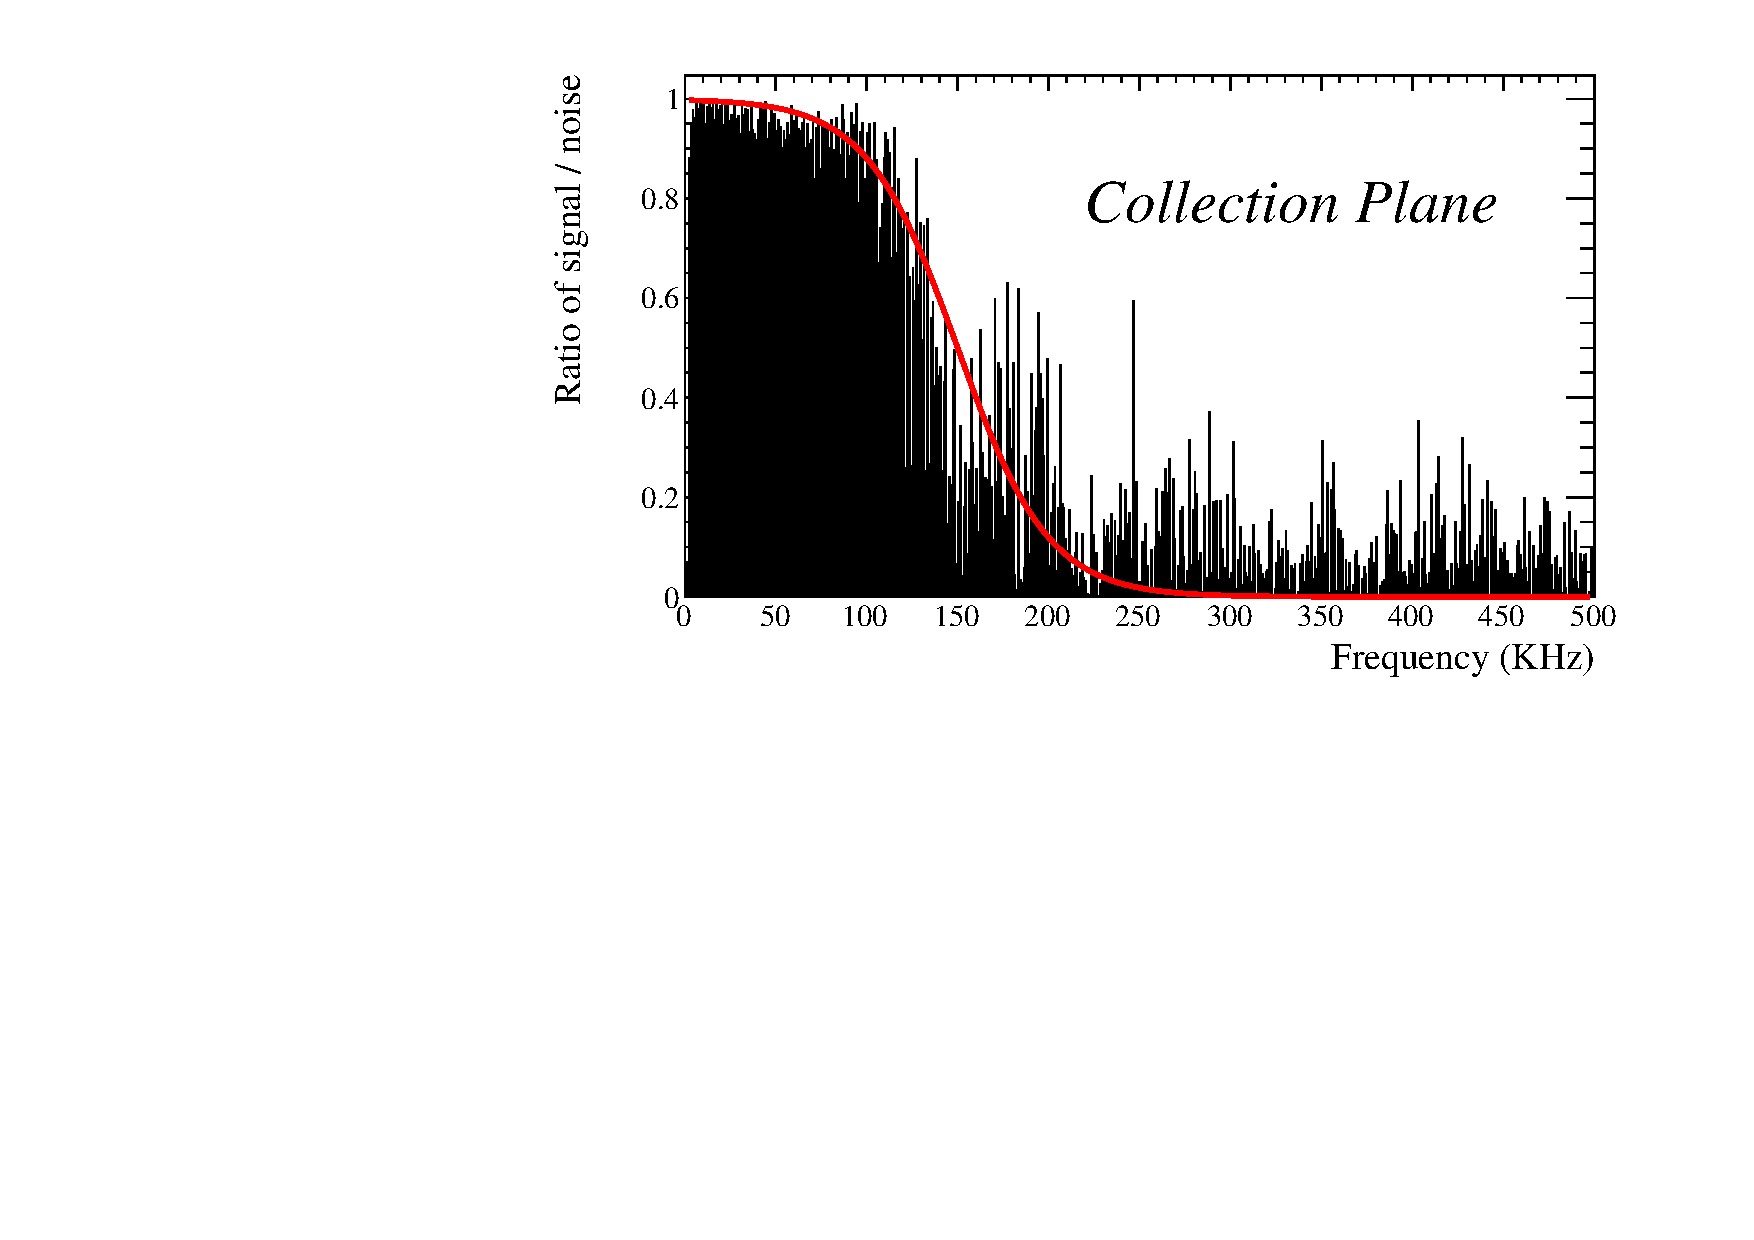
\includegraphics[width=\textwidth]{Collection}
    \caption{The $signal/noise$ ratio for a collection plane wire, the red line shows the fraction of frequency power which passes the filter.}
    \label{fig:FreqCollection}
  \end{subfigure}%
  \hspace{0.03\textwidth}%
  \begin{subfigure}{0.48\textwidth}
    \centering
    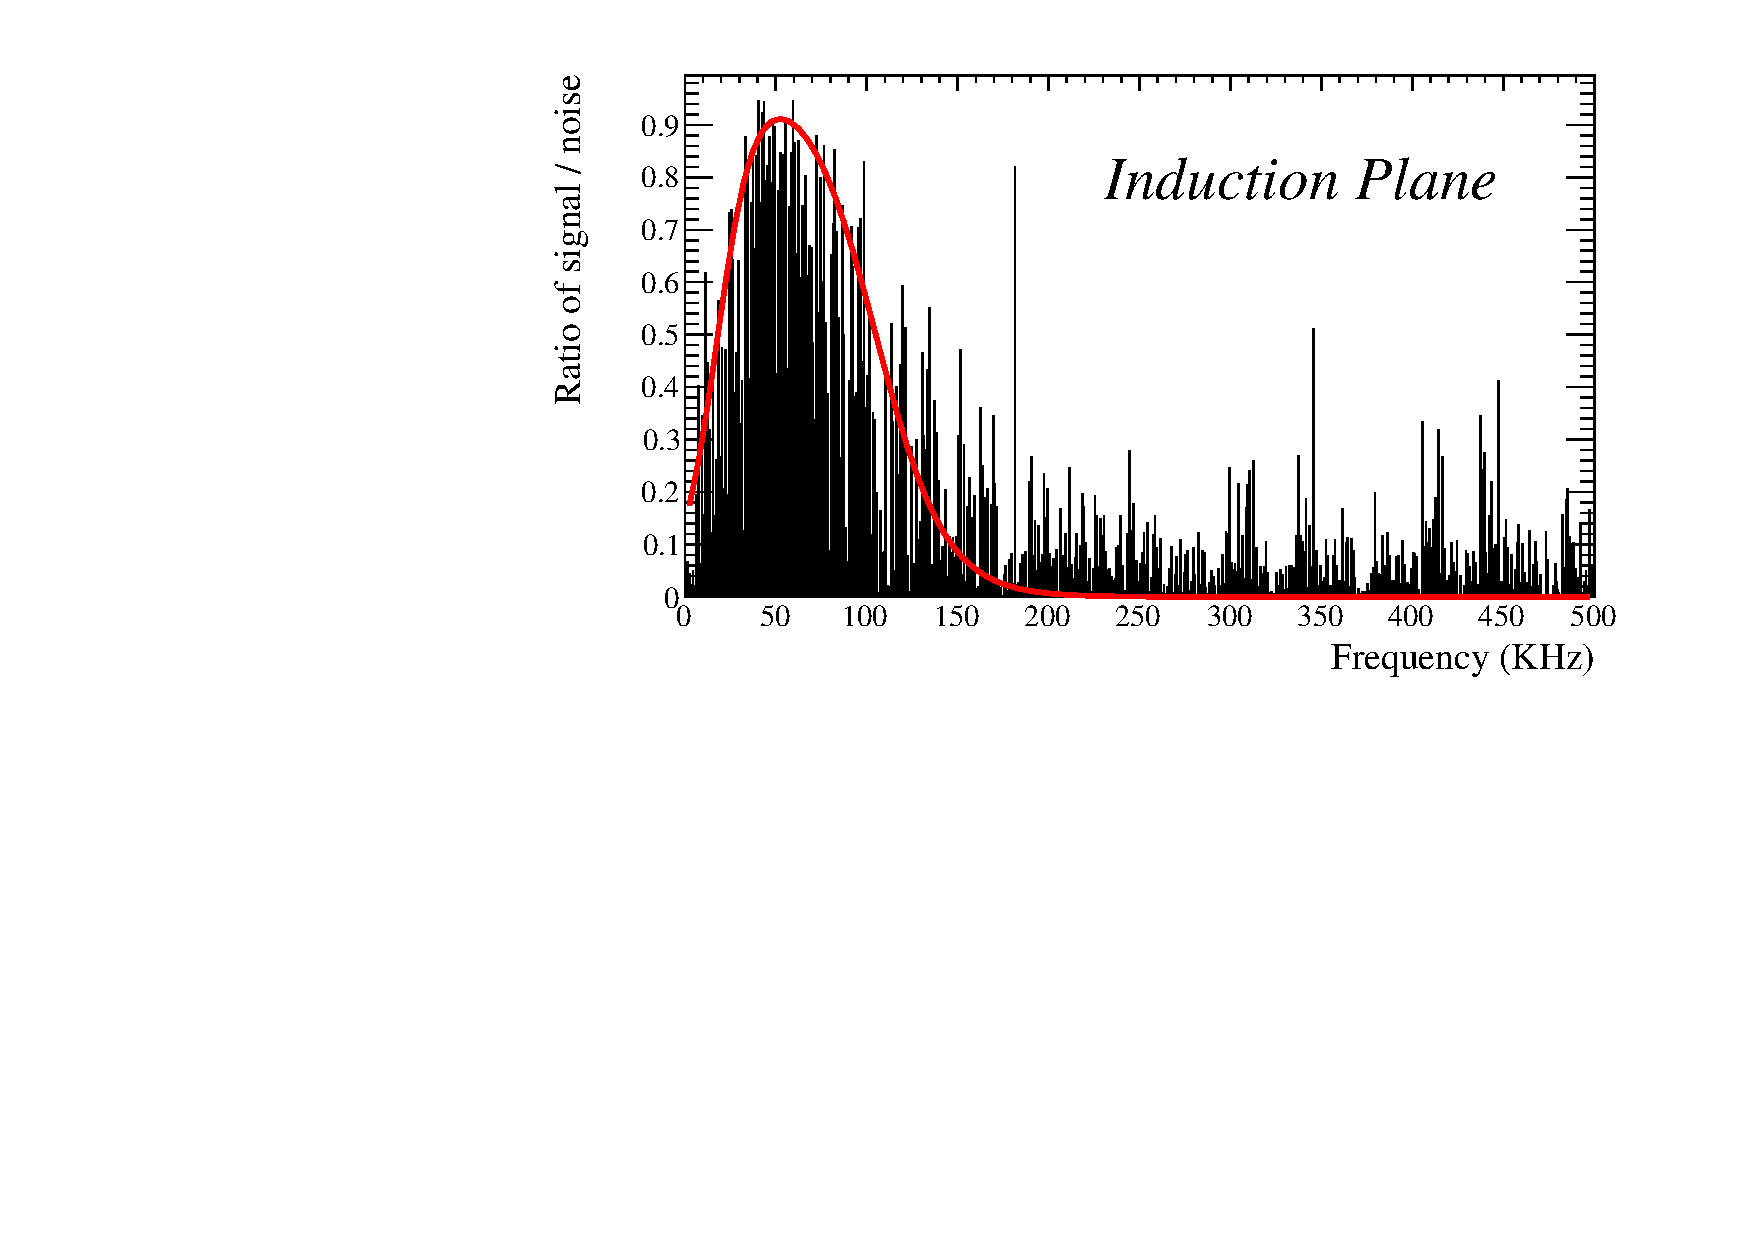
\includegraphics[width=\textwidth]{Induction}
    \caption{The $signal/noise$ ratio for an induction plane wire, the red line shows the fraction of frequency power which passes the filter.}
    \label{fig:FreqInduction}
  \end{subfigure}
  \caption[Applying Wiener filters to the 35 ton data]
          {The application of Wiener filters to the 35 ton data. Top left: a waveform from a collection plane wire which is then signal suppressed. Top right: the FFT of both the raw and signal suppressed waveforms. Bottom left: the $signal/noise$ ratio for the collection plane waveform, a sigmoid function has been overlaid to preserve the areas of high $signal/noise$, and suppress the areas of low $signal/noise$. Bottom right: the $signal/noise$ frequency space ratio for an induction plane wire, a sigmoid function has been overlaid to preserve only the areas of high $signal/noise$.}
  \label{fig:FrequencyFilter}
\end{figure}

An example of the effect of the noise mitigation steps is shown in Figure~\ref{fig:NoiseRemoval}. Figure~\ref{fig:NoiseRemoval_Raw} shows the raw data, whilst Figure~\ref{fig:NoiseRemoval_Mit} shows the data after the stuck code unsticker, coherent noise removal and Wiener filter algorithms have been applied. The effect of noise removal is clear, as the signals from the tracks become much more pronounced, particularly on the bottom induction plane. However, it can also be seen that the noise removal algorithms also remove signals from tracks, as the depositions seen on the collection plane in Figure~\ref{fig:NoiseRemoval_Raw} at around tick 10,000 becomes much less pronounced in Figure~\ref{fig:NoiseRemoval_Mit}. \\

\begin{figure}
  \centering
  \begin{subfigure}{0.55\textwidth}
    \centering
    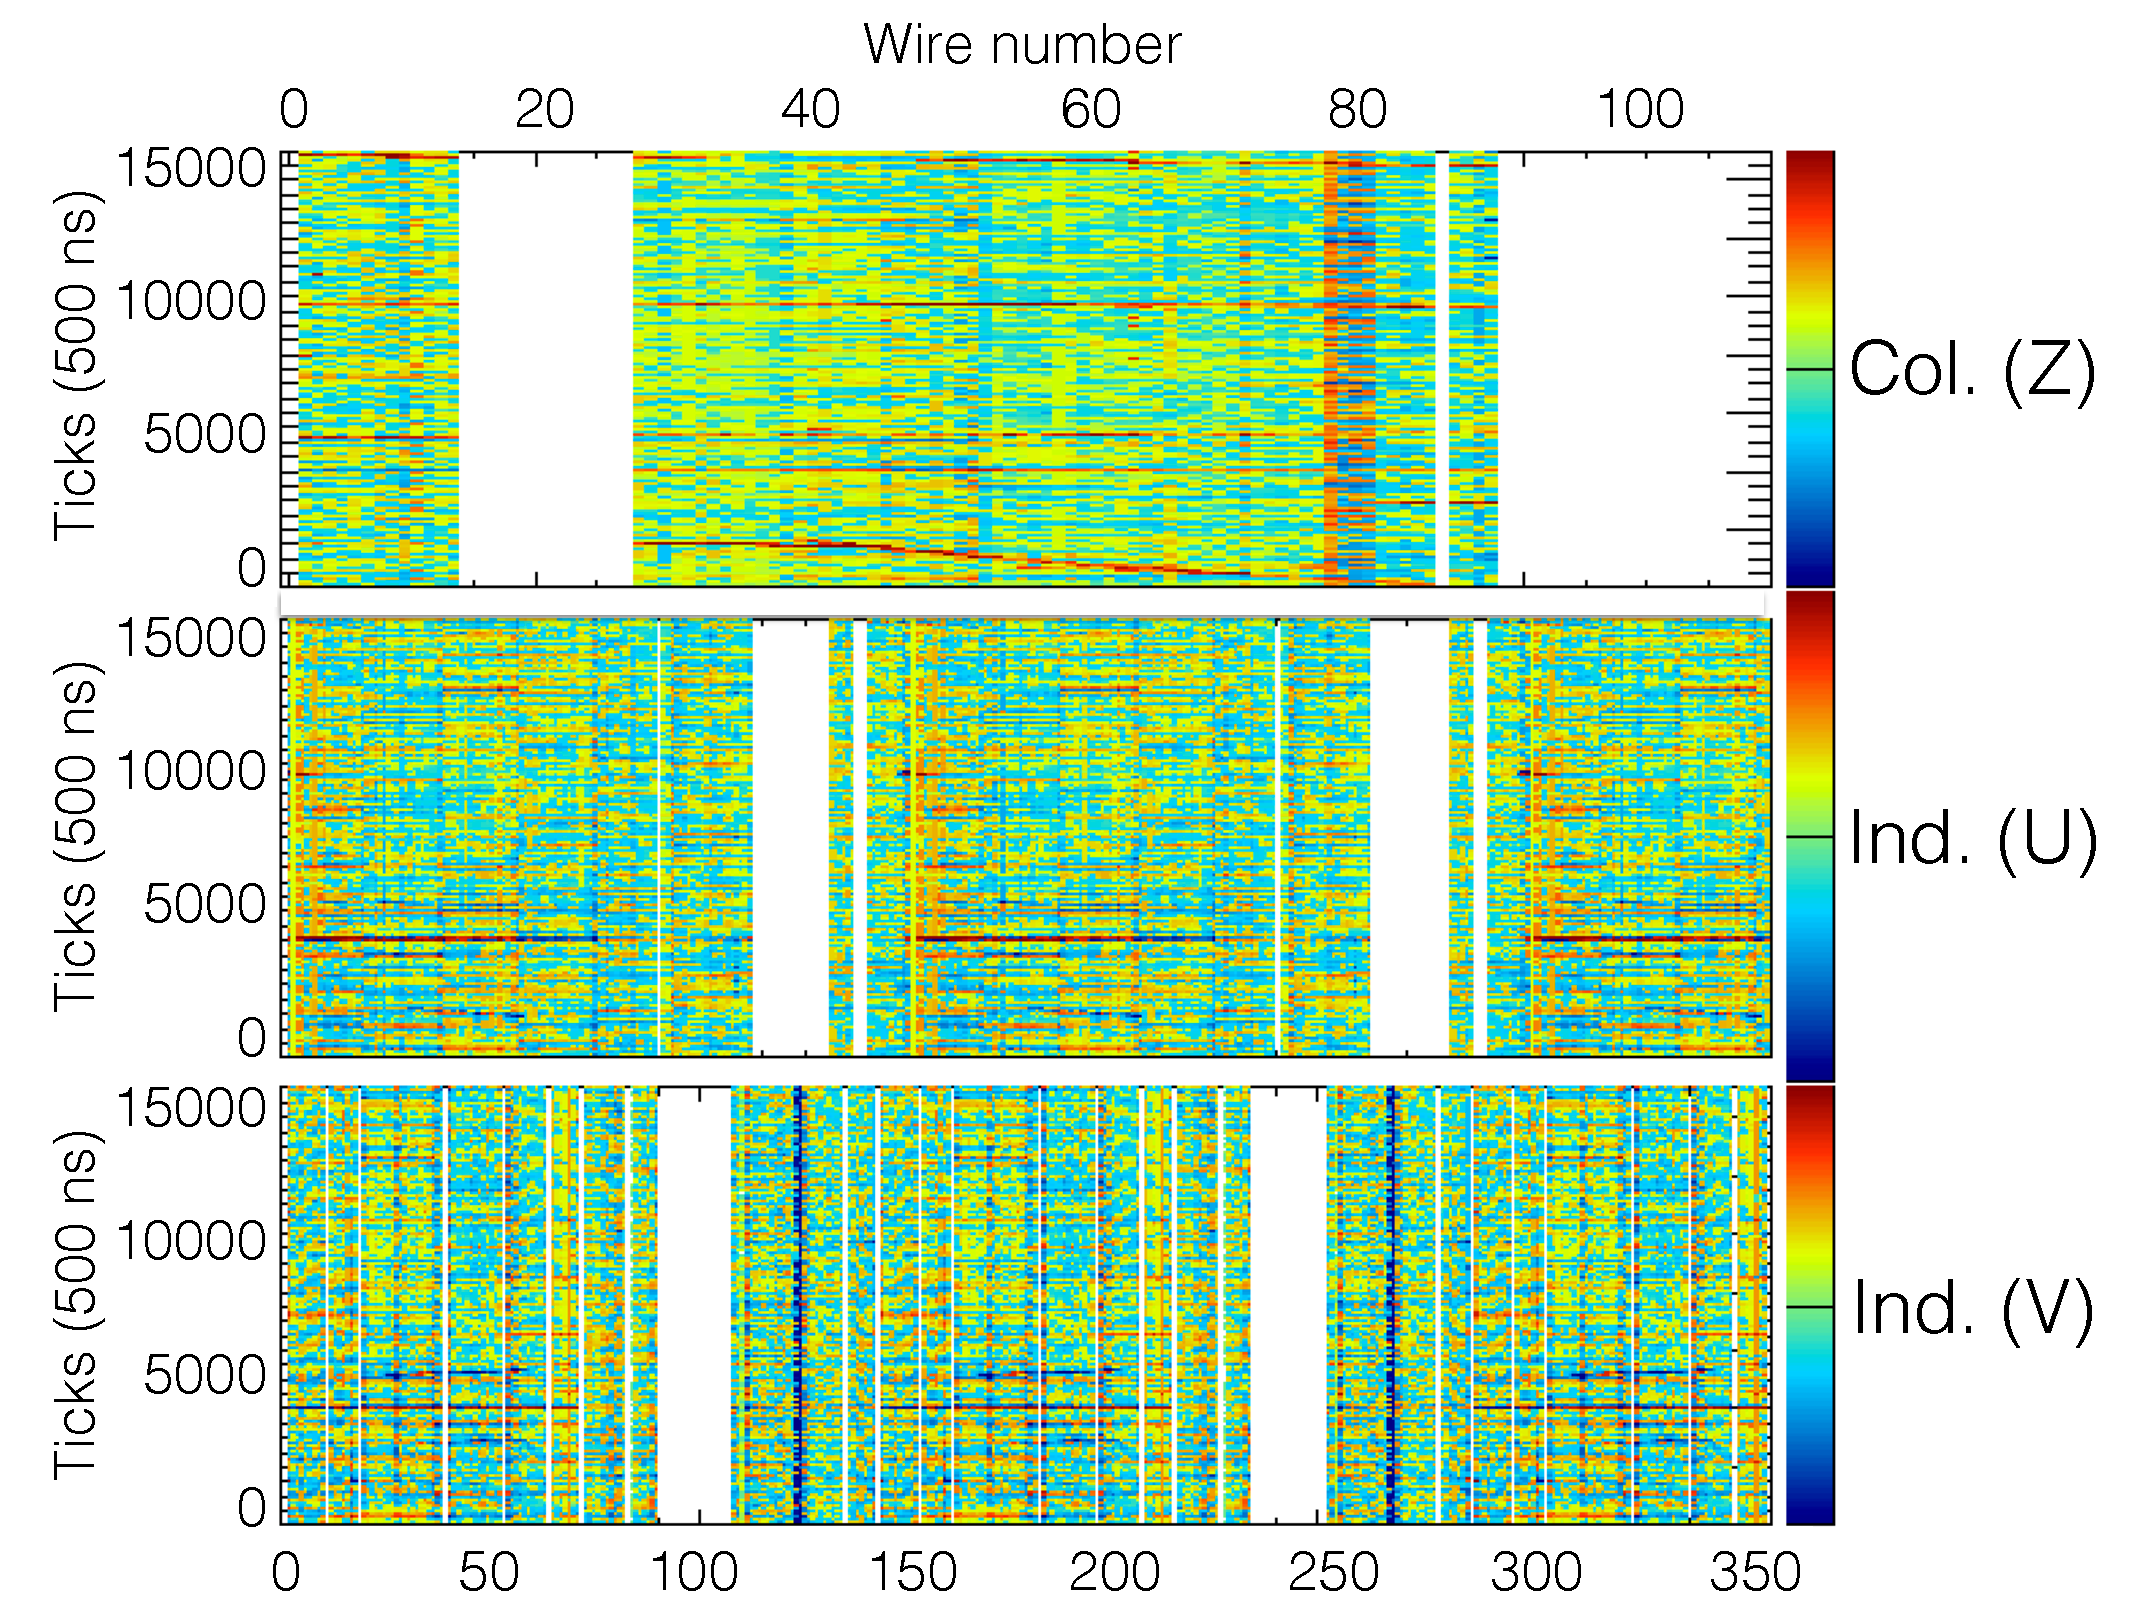
\includegraphics[width=\textwidth]{Evd_BeforeNoise}
    \caption{Raw signal before noise removal}
    \label{fig:NoiseRemoval_Raw}
  \end{subfigure}
  \begin{subfigure}{0.55\textwidth}
    \centering
    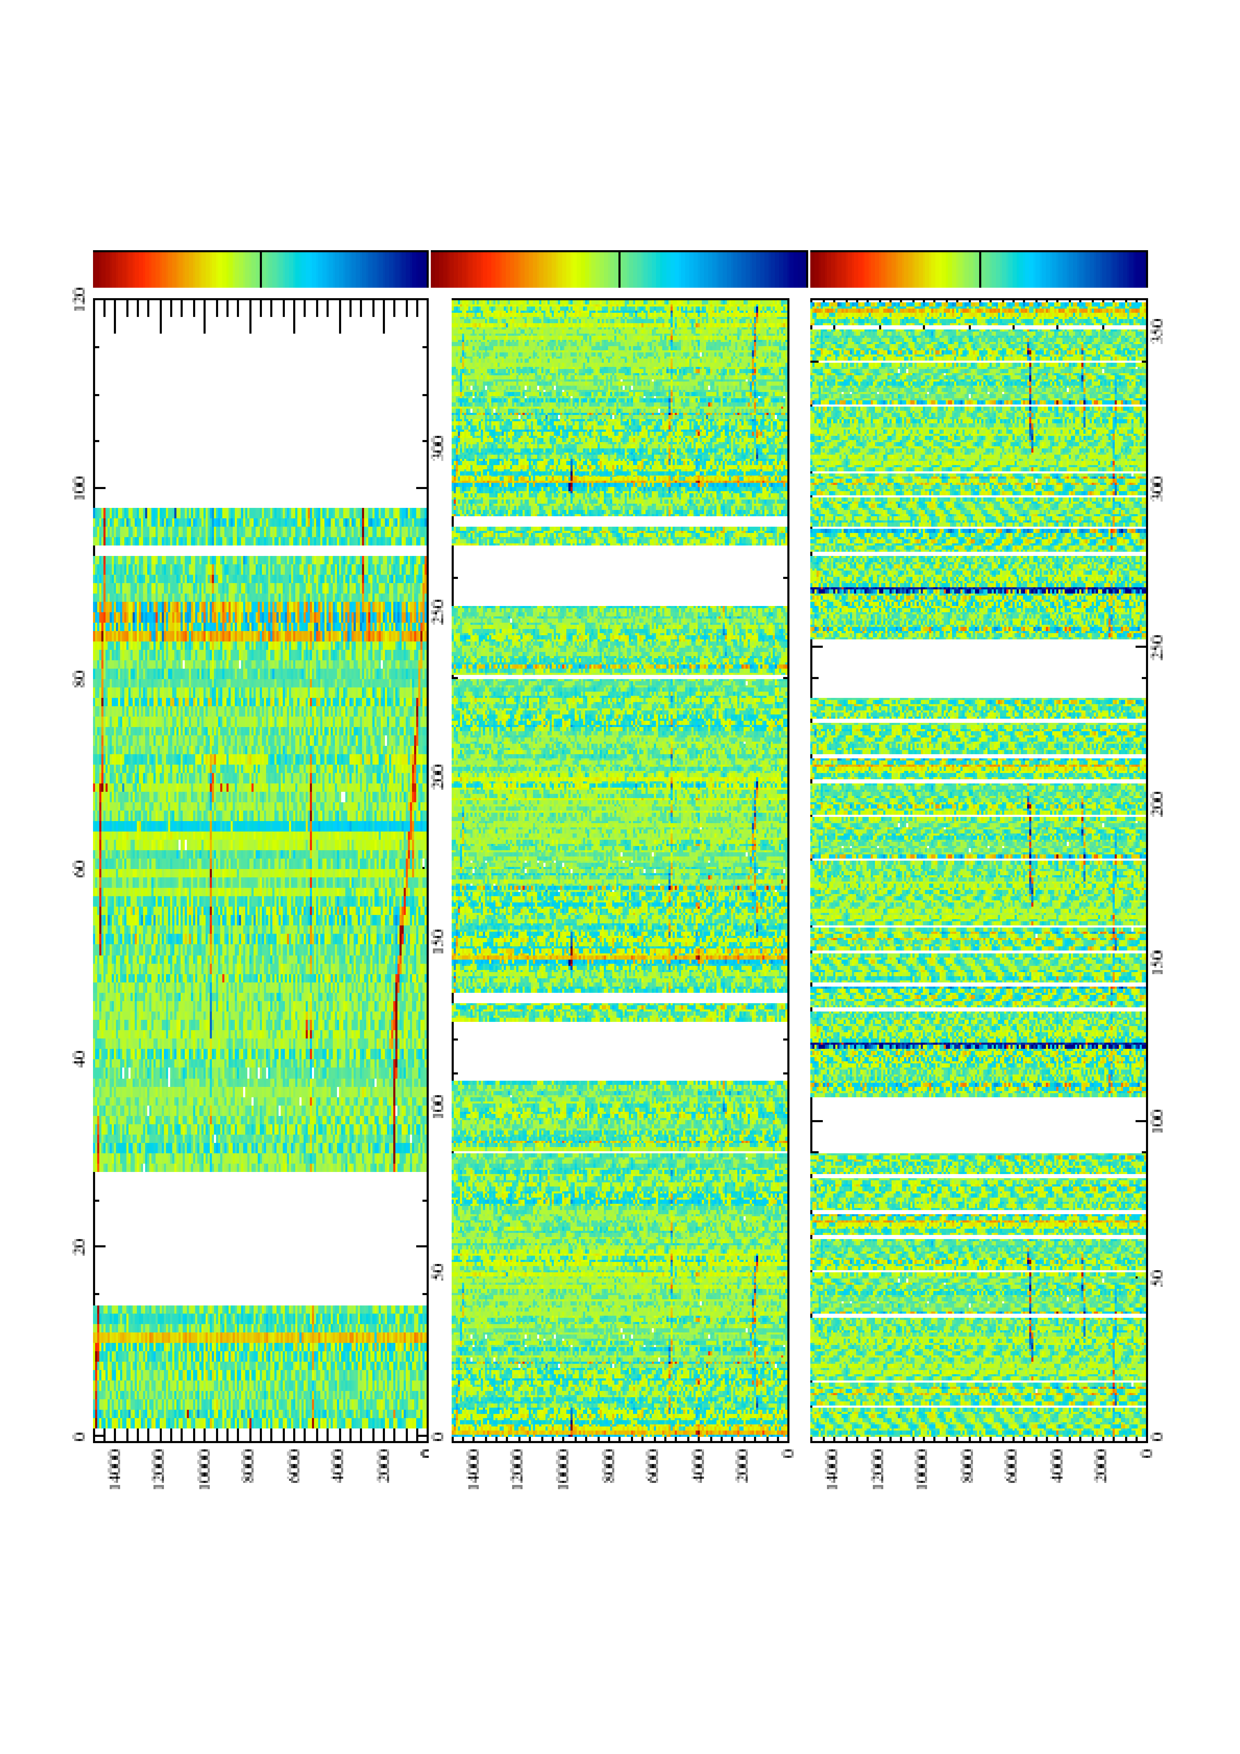
\includegraphics[width=\textwidth]{Evd_AfterNoise}
    \caption{Signal after noise removal}
    \label{fig:NoiseRemoval_Mit}
  \end{subfigure}
  \caption[The effect of noise removal algorithms in the 35 ton data]
          {Event displays showing the effect of the noise removal algorithms on data from the 35 ton detector. The event displays show the signals in the collection (Z), and induction planes (U and V). The plots show wire number, and time in ticks, on the $x$ and $y$ axes respectively. The charge is shown on the colour axis, where areas in red represent areas of high charge deposition, whilst blue represents areas of low charge deposition, areas of white show wires which did not read out any signals. The effect of the noise removal algorithms can clearly be seen, as large changes in charge due to the noise are no longer present after they have been applied. The application of the noise removal algorithms does however remove real signals, as the number of depositions across many channels around tick 10,000 on the collection plane are noticeably reduced after they are applied.}
  \label{fig:NoiseRemoval}
\end{figure}

Transitions to a higher noise state were observed after cool down, this was associated with strong signals at frequencies between 400 and 650 KHz. The transitions would occur approximately every 2 hours, and were occasionally observed to happen shortly after a saturation event across the whole detector~\citep{35tonNoiseMeeting}. Once the state was induced, the only way to stop it was to power cycle the low voltage supplies. It was found that power cycling the short APA at the base of the detector (APA2) could both stop, and induce the higher noise state. Importantly, this was the only APA with electronics located at the base of the TPC. The data taken during the elevated noise state was unrecoverable, as the electronics noise was too large, and so upon the observation of a transition, the low voltage supplies were power cycled. It was observed that the transitions occurred much less frequently when APA2 was not powered, and so it was not used for significant portions of the data taking period. Despite efforts to study the transitions during warm testing they were unable to be induced, and have not been observed in other experiments such as MicroBooNE, despite the same low voltage supplies being used. It is thought that the cause of the transitions is a feedback loop in the low voltage cable, which was much longer in the 35 ton than in MicroBooNE. This would explain why APA2 was more susceptible to the feedback loop, as the cable is routed past its electronics~\citep{35tonNoiseDoc}.

%********************************** % Fourth Section  *************************************
\section{Performance of reconstruction algorithms} \label{sec:DataAlgs}  %Section - X.4
After performing the noise removal which was outlined in Section~\ref{sec:AllTheNoise}, hit and track finding was still more difficult than in simulations, due to the elevated noise level. In order for a reasonable number of hits to be reconstructed the hit finding threshold had to be substantially increased in data, as compared to Monte Carlo. This meant that many of the low energy hits would not be reconstructed. \\

A potential solution to not reconstructing the low energy hits, is to use the counter positions to select only hits which could have caused coincidences. When determining whether a reconstructed hit could have caused the counter coincidence, a two-dimensional window around the counter edges in the $yz$ plane is constructed, and timing information is used to extend this to three dimensions. The $x$ position of the hit can be calculated using the hit time, and electron drift velocity using Equation~\ref{eq:HitTime}. \\

Determining whether collection plane hits are within the counter window is trivial as they have a constant $z$ position, and either cover the full detector height (tall APAs), or roughly half of the detector height (short APAs). However, the wrapping of the induction planes, means that each wire segment has to be considered individually, and that multiple segments of a given wire could lie within the counter shadow. The 3-dimensional volume that is enclosed by connecting the edges of the counters which were hit in the counter coincidence, is called the ``counter shadow.'' Only those wires which lie within the 2-dimensional projection of this volume onto the $yz$ plane, are considered here. Choosing between these potential wire segments is done by iterating through the following steps. If at any point only one segment satisfies a given condition, then that segment is chosen:
\begin{itemize}
\item Does the wire segment intersect any collection plane wires which record hits?
  \begin{itemize}
  \item This is because when there is a signal on an induction plane there should also be signals on the collection wires.
  \end{itemize}
\item Are there adjacent wires which have hits at a similar time?
  \begin{itemize}
  \item This is because one would expect a track to deposit energy on multiple adjacent wire segments. 
  \end{itemize}
\item Which hit lies closest to the line defined by unique collection plane hits in the $xz$ plane?
  \begin{itemize}
  \item This is follows identical logic to the first criterion, but selects the hit which best matches the collection plane hits, and attempts to remove the effect of noisy collection plane wires by only using wires which have one hit within the counter shadow. This would also hopefully improve the quality of the fit, as there will not be numerous outlying hits.
  \item This can be changed to consider the line defined by previously selected hits in the given TPC and plane where the hit choices are.
  \end{itemize}
\end{itemize}

Following a re-optimisation of the clustering algorithms, it was observed that the standard reconstruction could achieve track reconstruction to a similar efficiency as the counter shadowing method, and so the standard reconstruction has been used in the discussions to follow~\citep{TingjunClustering}. There has since been an effort to improve the counter shadowing hit disambiguation to remove the outlying collection plane hits using the MLESAC method~\citep{MLESAC}, whereby points which are far away from a best fit are ignored. These studies are still on-going~\citep{MattMLESAC}. \\

%****** Now to talk about the reconstruction efficiencies... ******%
A symptom of the elevated noise state is that signals are often dropped on one of the induction planes, this means that the tracking algorithms often have to combine clusters in only two of the three planes. Reconstruction using two planes was shown to be effective by the ArgoNeuT collaboration~\citep{ArgoNeuT}, so the loss of signal in one of the three planes is not prohibitive to track reconstruction. Another consequence of the elevated noise level is that even when the counters are used to seed hit finding, the hit finding threshold is too high to reconstruct the very lowest hits. This causes the plot of $dQ/dx$ for muons, shown in Figure~\ref{fig:TingjunLifetime}, to look flat, due to a cutoff at 100~ADC$\cdot$cm$^{-1}$, below which no hits are reconstructed. The inability to reconstruct the lowest energy hits means that calorimetry is all but impossible on the 35 ton dataset, even though the tracking algorithms perform relatively well. The inability to perform reliable calorimetry en masse means that the only particles which can be assuredly identified are the muons which triggered the counter coincidences. This means that performing the analysis that was presented in Section~\ref{sec:PID} on the 35 ton dataset is extremely difficult, if not impossible. \\

\begin{figure}
  \centering
  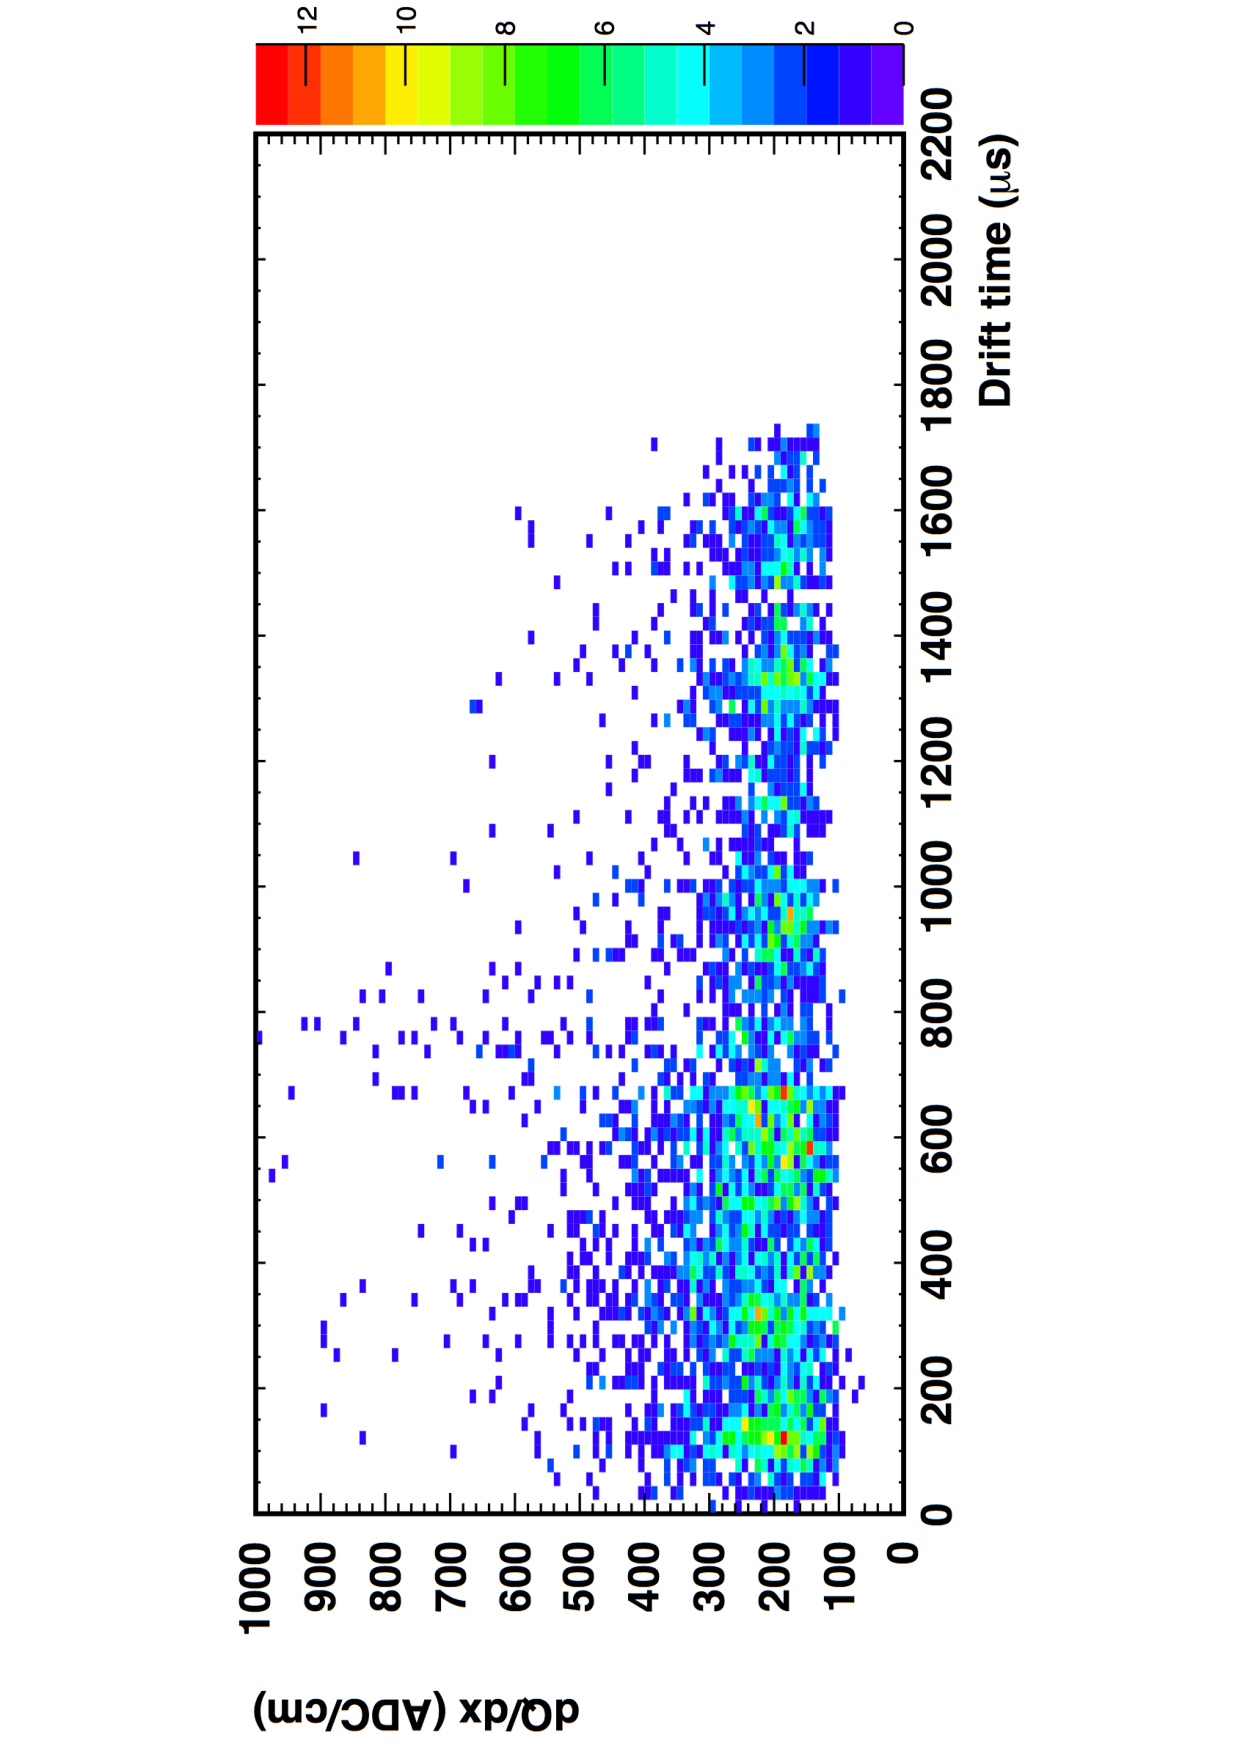
\includegraphics[width=0.85\textwidth]{TingjunLifetime}
  \caption[$dQ/dx$ in the 35 ton as a function of drift time]
          {The $dQ/dx$ values for a sample of muon collection plane hits, note the cutoff at 100~ADC$\cdot$cm$^{-1}$ due to the hit finding threshold. The figure is taken from~\citep{TingjunLifetime}.}
  \label{fig:TingjunLifetime}
\end{figure}  

The muons in the triggered sample will all traverse the detector, but their orientations can be carefully selected by the user. For example, one could easily select a sample of muons which cross the APAs at increasing angles, or are parallel to the wire planes at increasing drift distances. This is done by matching through-going muons with counter coincidences. The process by which this is done is identical for both north-south and east-west coincidences, though more focus will be given to the later, as it is with muons of this orientation that the analysis presented in Section~\ref{sec:DiffusionAnalysis} was performed. The same matching technique would also have been applied to vertical muons had the telescope trigger been utilised. For a reference as to the locations of the counters around the cryostat, see Figure~\ref{fig:35tonCounterLoc}, and for a representation of only the east-west counters, see Figure~\ref{fig:EWCounters}. \\

\begin{figure}
  \centering
  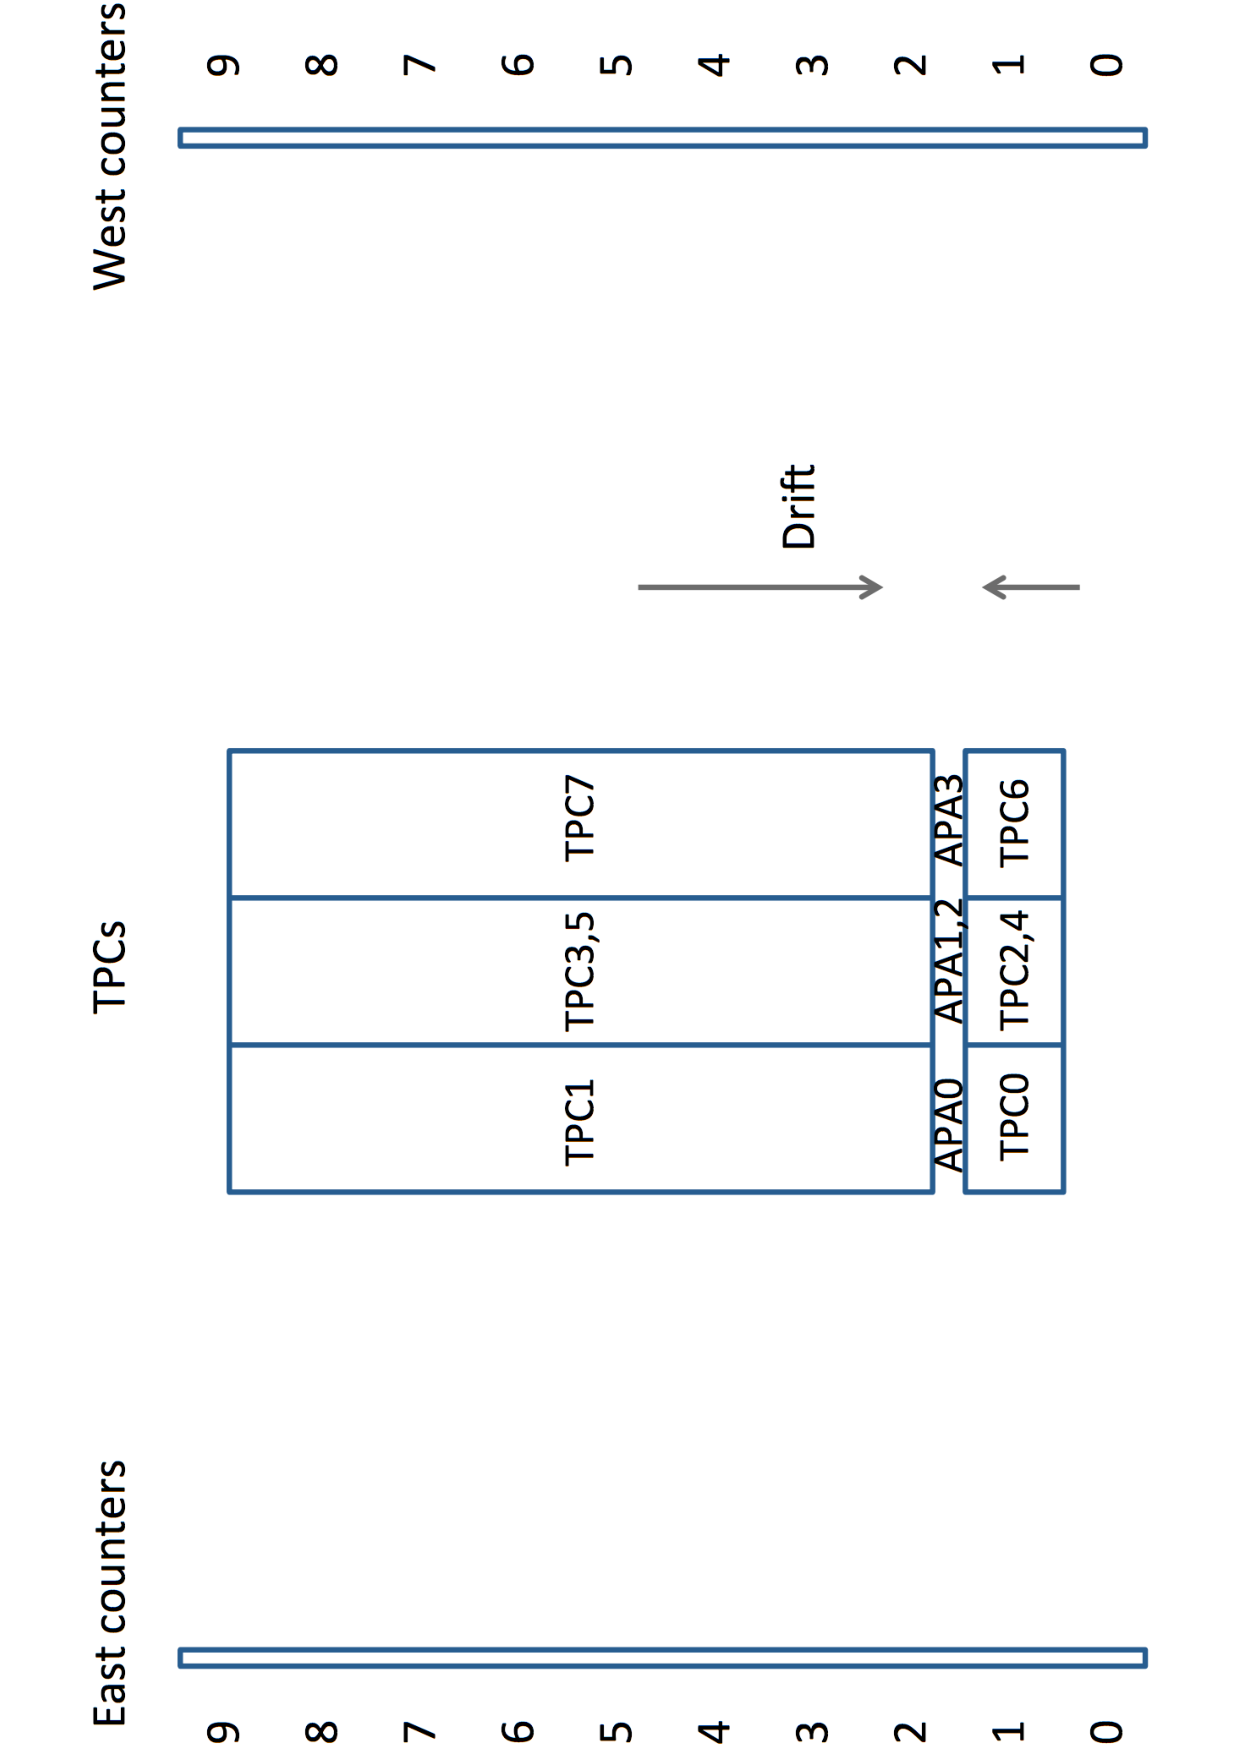
\includegraphics[width=0.65\textwidth]{CounterSchematic}
  \caption[The numbering scheme for the east - west counters in the 35 ton]
          {The numbering scheme for the east - west counters in the 35 ton. The counters have been numbered from 0 to 10 depending on their position from the end of the short drift volume. This is different to the LArSoft numbering scheme shown in Figure~\ref{fig:35tonCounterLoc} where they go from 6-15 and 28-37 for the east and west counters respectively. Three hypothetical muons which would have caused coincidence triggers are shown as dashed lines, and the hypothetical reconstructed tracks they produce are shown as solid lines. The red particle is an APA crossing event, and would produce tracks in TPCs 1 and 6. The black particle is fully reconstructed as one continuous track, however the blue particle is not reconstructed in the middle TPCs and so is reconstructed as two separate tracks.}
  \label{fig:EWCounters}
\end{figure}

It is possible to construct a line in the $yz$ plane joining the centres of the two counters which were hit when a coincidence occurred. This can then be compared with the trajectory of a track in the $yz$ plane, and the dot product of the two vectors calculated. A reconstructed track is assigned to a given counter coincidence if the dot product of the track and the coincidence is more than 0.98, and the hit times are consistent with the $x$ positions of the counters. The results of the dot product calculation are shown in Figure~\ref{fig:CounterCoincidence}. Matching only tracks which are well aligned with a counter coincidence should produce a pure sample of tracks, as parallel muons are unlikely to be highly correlated in time, and any tracks reconstructed from the noise will have random directions. This is shown in data where if multiple tracks pass the dot product cut they are co-linear, and are not randomly orientated, as shown in Figure~\ref{fig:CounterTrackAngle}. \\

\begin{figure}
  \centering
  \begin{subfigure}{0.48\textwidth}
    \centering
    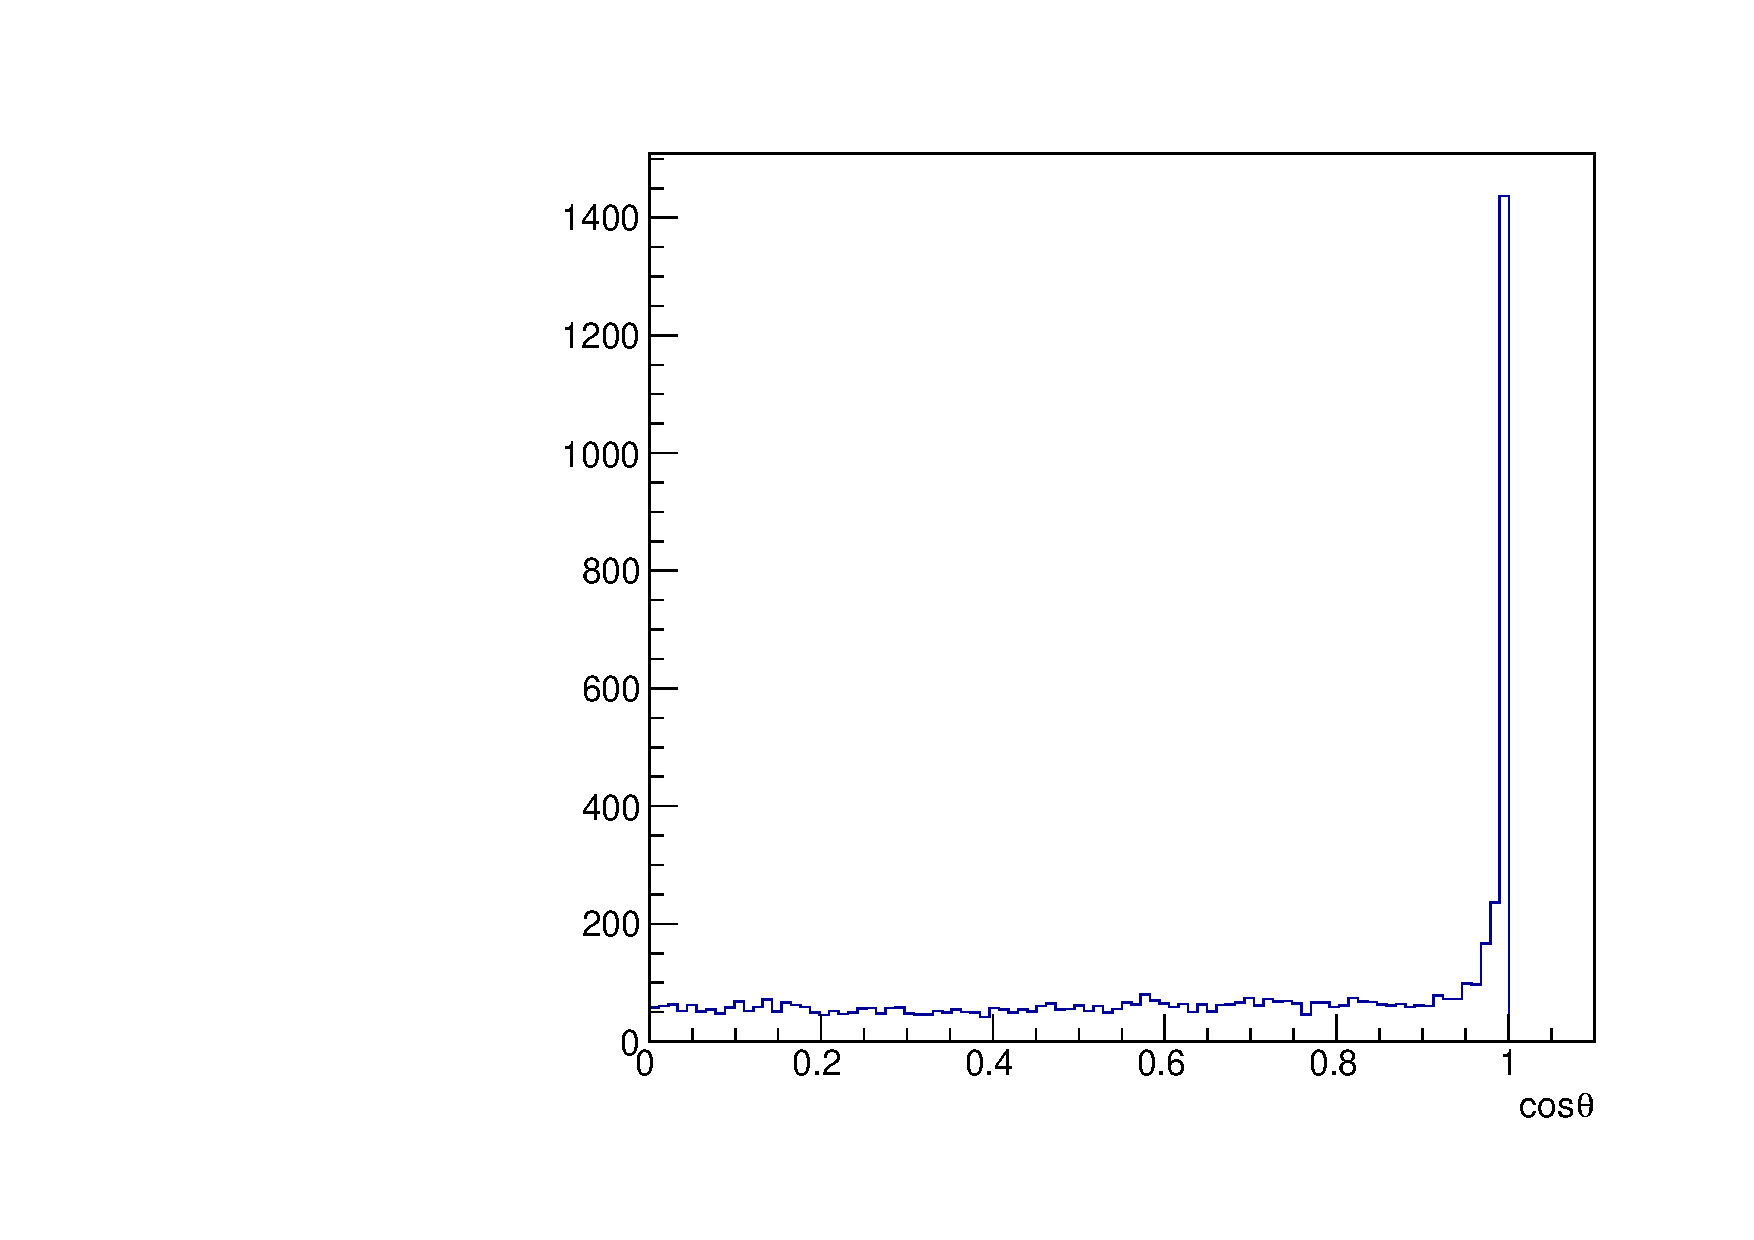
\includegraphics[width=\textwidth]{CosTheta_Data}
    \caption{All dot product values.}
  \end{subfigure}%
  \hspace{0.03\textwidth}%
  \begin{subfigure}{0.48\textwidth}
    \centering
    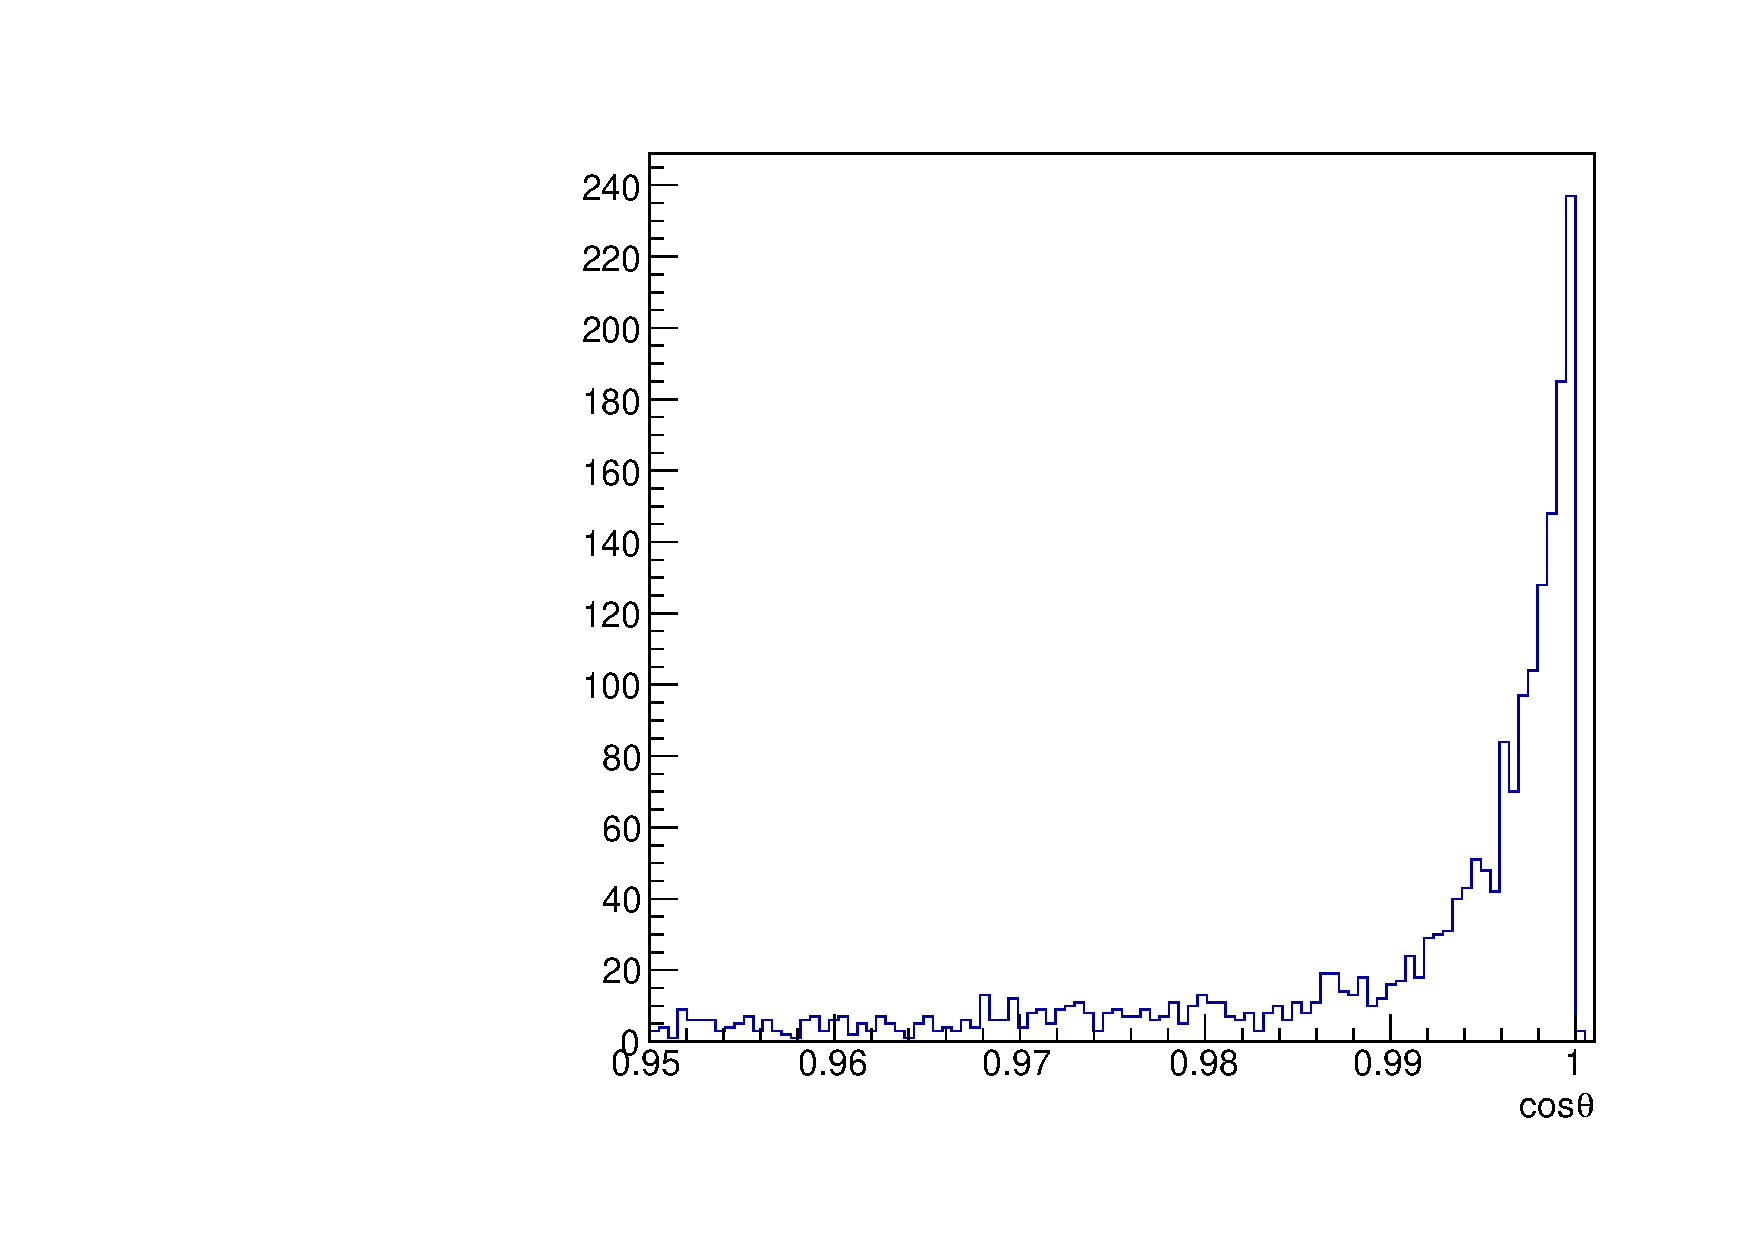
\includegraphics[width=\textwidth]{CosThetaZoom_Data}
    \caption{Dot product values close to 1.}
  \end{subfigure}
  \caption[The dot product of the track and vector joining the centres of the coincidence counters in the $yz$ plane]
          {The dot product of the track and vector joining the centres of the coincidence counters in the $yz$ plane. The number of tracks with a given dot product is plotted on the $y$ axis. A threshold value of 0.98 is required for a track to be considered to be due to the counter coincidence. It can be seen that many tracks are well aligned with counter coincidences, having dot products of more than 0.99.}
          \label{fig:CounterCoincidence}
\end{figure}

\begin{figure}
  \centering
  \begin{subfigure}{0.48\textwidth}
    \centering
    \includegraphics[width=\textwidth]{north-south}
    \caption{A north-south counter coincidence.}
  \end{subfigure}%
  \hspace{0.03\textwidth}%
  \begin{subfigure}{0.48\textwidth}
    \centering
    \includegraphics[width=\textwidth]{east-west}
    \caption{An east-west counter coincidence.}
  \end{subfigure}
  \caption[The alignment of reconstructed tracks with the vectors joining the centres of the coincidence counters]
          {The alignment of reconstructed tracks with the vectors joining the centres of the coincidence counters. The dashed lines show the vectors joining the centres of counters hit in the coincidence, whilst the solid lines show the reconstructed tracks. Left: the alignment of tracks with a north-south coincidence. Right: the alignment of tracks with an east-west coincidence. The $z$ positions of the tracks are shown on the $x$ axis, and the $y$ positions of the tracks are shown on the $y$ axis. The figures were taken from~\citep{TingjunClustering}.}
          \label{fig:CounterTrackAngle}
\end{figure}

By matching tracks in this way it is possible to evaluate the reconstruction efficiencies for these muons, at increasing drift distances and track angles. If multiple tracks are aligned with the coincidence, and are within the expected time region, then their track lengths are summed when calculating reconstruction efficiencies. When this occurs, it is expected that the track was split by a region of the detector either being turned off, or being too noisy to reconstruct a track. If these tracks have a combined track length of more than 50~cm, then the coincidence is identified as having been successfully reconstructed. This threshold is much lower than the true track length which should be reconstructed (more than 150~cm), but few particles are fully reconstructed in the data, and so a compromise is made to achieve a large enough sample of tracks upon which analyses can be performed. A reconstructed track that is 50~cm long is likely to have a large number of hits on collection plane wires that are not noisy, and it is these hits which are required when calculating purity or measuring the effect of diffusion, as discussed in Section~\ref{sec:DiffusionAnalysis}. A track with length more than 50~cm is also likely to have been stitched between TPCs, due to the geometry of the 35 ton and track trajectories. The demonstration of stitching tracks between TPCs was a design goal of the 35 ton, and so identifying tracks where this was achieved satisfies that goal. \\

An important concept that must be introduced before these reconstruction efficiencies can be described is that of a ``counter difference.'' The ``counter difference'' of a coincidence and it's associated tracks, is defined as the absolute difference between the counter numbers of the east and west counters that were hit. As such, the ``counter differences'' of the coincidences shown in Figure~\ref{fig:CounterCoincidence}, are 2, 3 and 6 for the black, red and blue coincidences respectively. Given the orientation of the counters, the rarest counter difference will be 9, as only particles which hit counters ($E_0$ and $W_9$) and ($E_9$ and $W_0$) will have a counter difference of 9. In contrast to this, the most common value for the counter difference is 1, as there are many possible combinations of east and west counters being hit to give this counter difference. In the discussions below ``counter difference'' is occasionally referred to as ``delta counter'' or ``$\Delta$ counter.'' Table~\ref{tab:CDiffAng} shows the approximate angles which tracks, with given counter differences, have relative to the APA frames. \\

\begin{table}
\caption[The angles which tracks, with given counter differences, have relative to the APA frames]
        {The angles which tracks, with given counter differences, have relative to the APA frames. Though the east and west counters have a width in the $y$ (vertical) direction, this is much less than their extent in the $z$ direction. The depth of the counters, their extent in $x$, is negligible compared to the separation of the east-west counters. The counters have identical widths in both the $y$ and $z$ directions. The angles are calculated using the difference in the centres of the counters in the $z$ direction, divided by the separation of the east and west counters in $z$.}
\centering
\label{tab:CDiffAng}
\begin{tabular}{c c}
\toprule
{Absolute counter difference} & {Approximate angle ($^{\circ}$)} \\ 
\midrule
0 & 0    $\pm$ 2.1 \\

1 & 4.2  $\pm$ 2.1 \\

2 & 8.4  $\pm$ 2.0 \\

3 & 12.5 $\pm$ 2.0 \\

4 & 16.5 $\pm$ 2.0 \\

5 & 20.3 $\pm$ 1.9 \\

6 & 23.9 $\pm$ 1.8 \\

7 & 27.3 $\pm$ 1.7 \\

8 & 30.7 $\pm$ 1.6 \\

9 & 33.5 $\pm$ 1.5 \\
\bottomrule
\end{tabular}
\end{table}

Figure~\ref{fig:DataRecoEffics} shows a range of reconstruction efficiency plots for combinations of different counter differences, and different drift distances. As the counter coincidences with large counter differences will have large variations in drift positions, the drift distance plotted here is the average $x$ position of the counter centres that were hit. For example, if the two counters that produced the coincidence are at $x$ = 10~cm and $x$ = 230~cm respectively, then the drift distance plotted would be 120~cm. This distance is called the ``coincidence centre'' in the following discussion. Only coincidences which would produce tracks that are contained within the long drift volume are considered here, hence there being no negative $x$ positions. \\

\begin{figure}
  \centering
  \begin{subfigure}{0.65\textwidth}
    \centering
    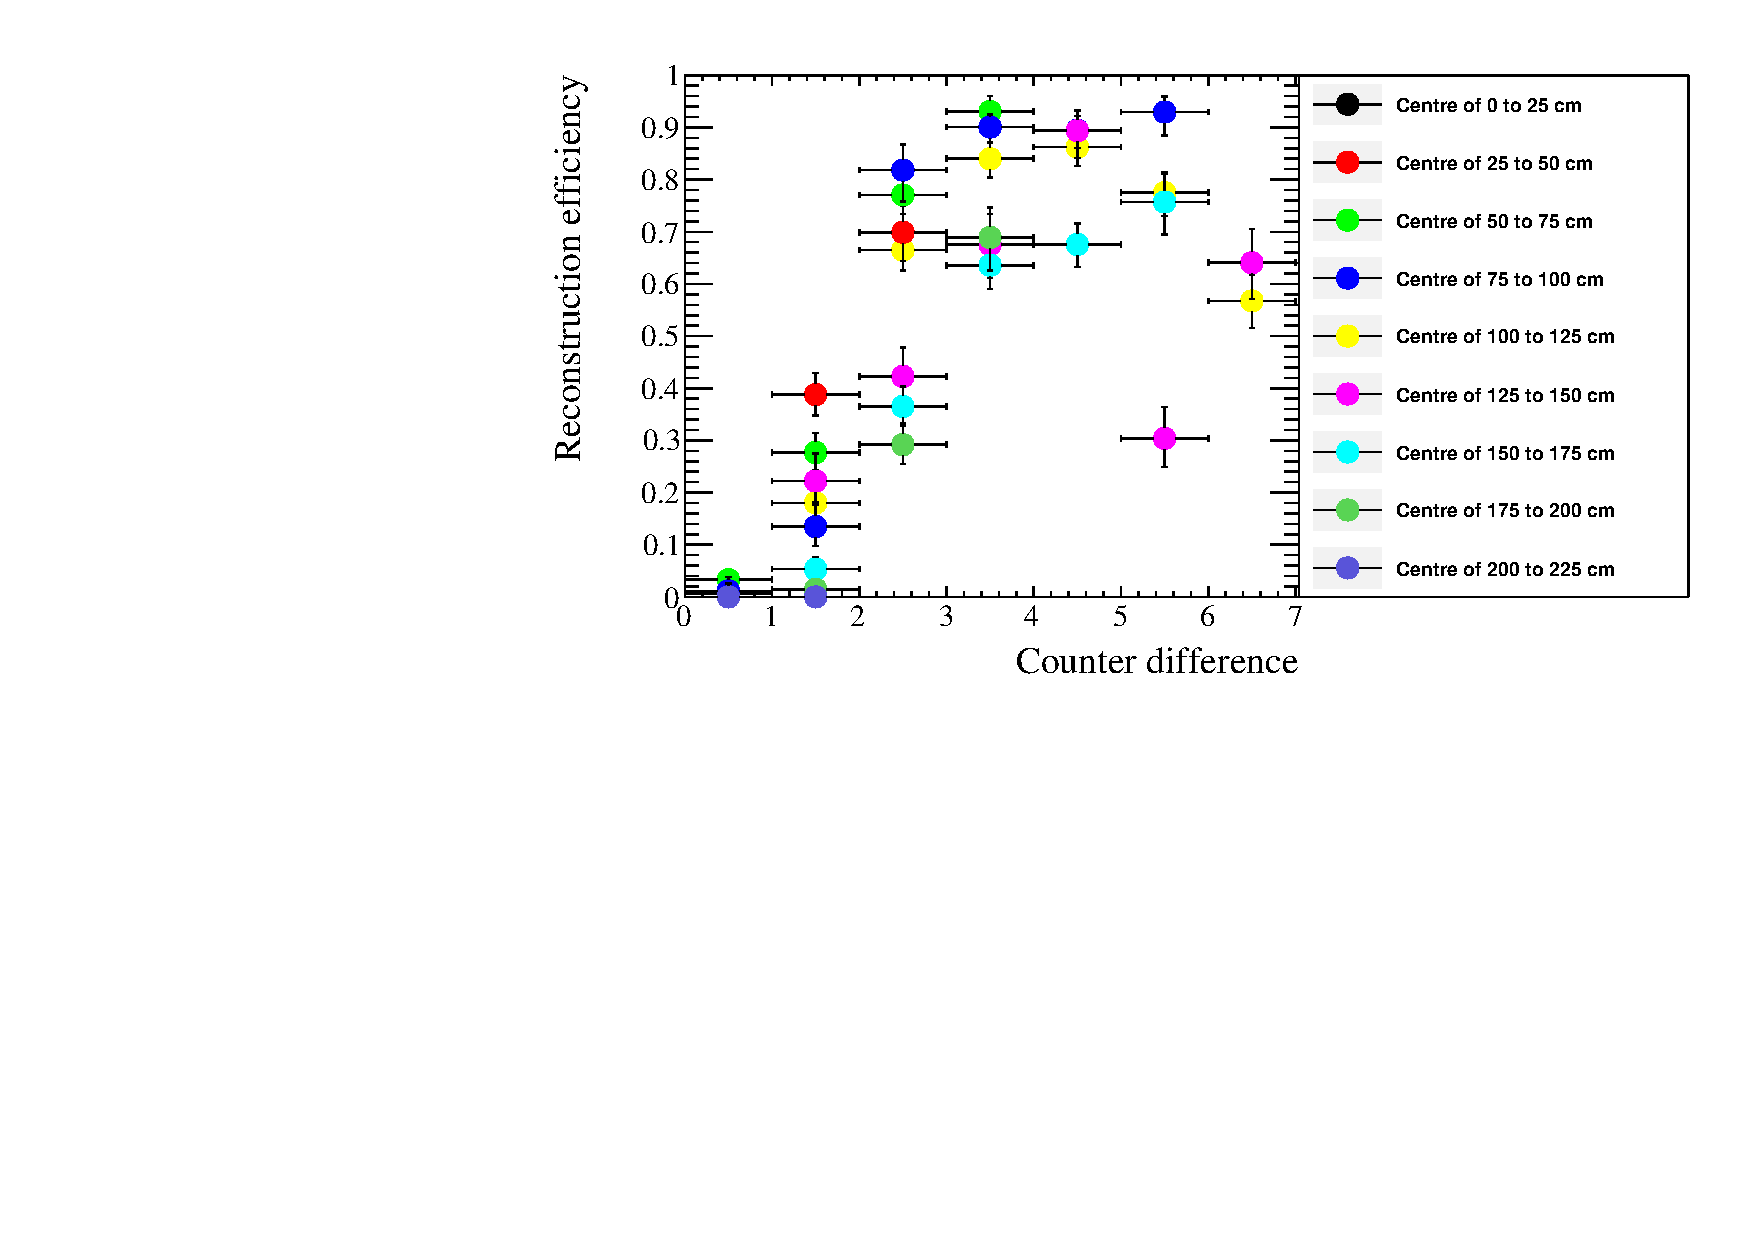
\includegraphics[width=\textwidth]{AngleCanvas_50}
    \caption{The reconstruction efficiency as a function of counter difference for different coincidence centres.}
    \label{fig:AngleCanvas}
  \end{subfigure}
  %\hspace{0.03\textwidth}%
  \begin{subfigure}{0.65\textwidth}
    \centering
    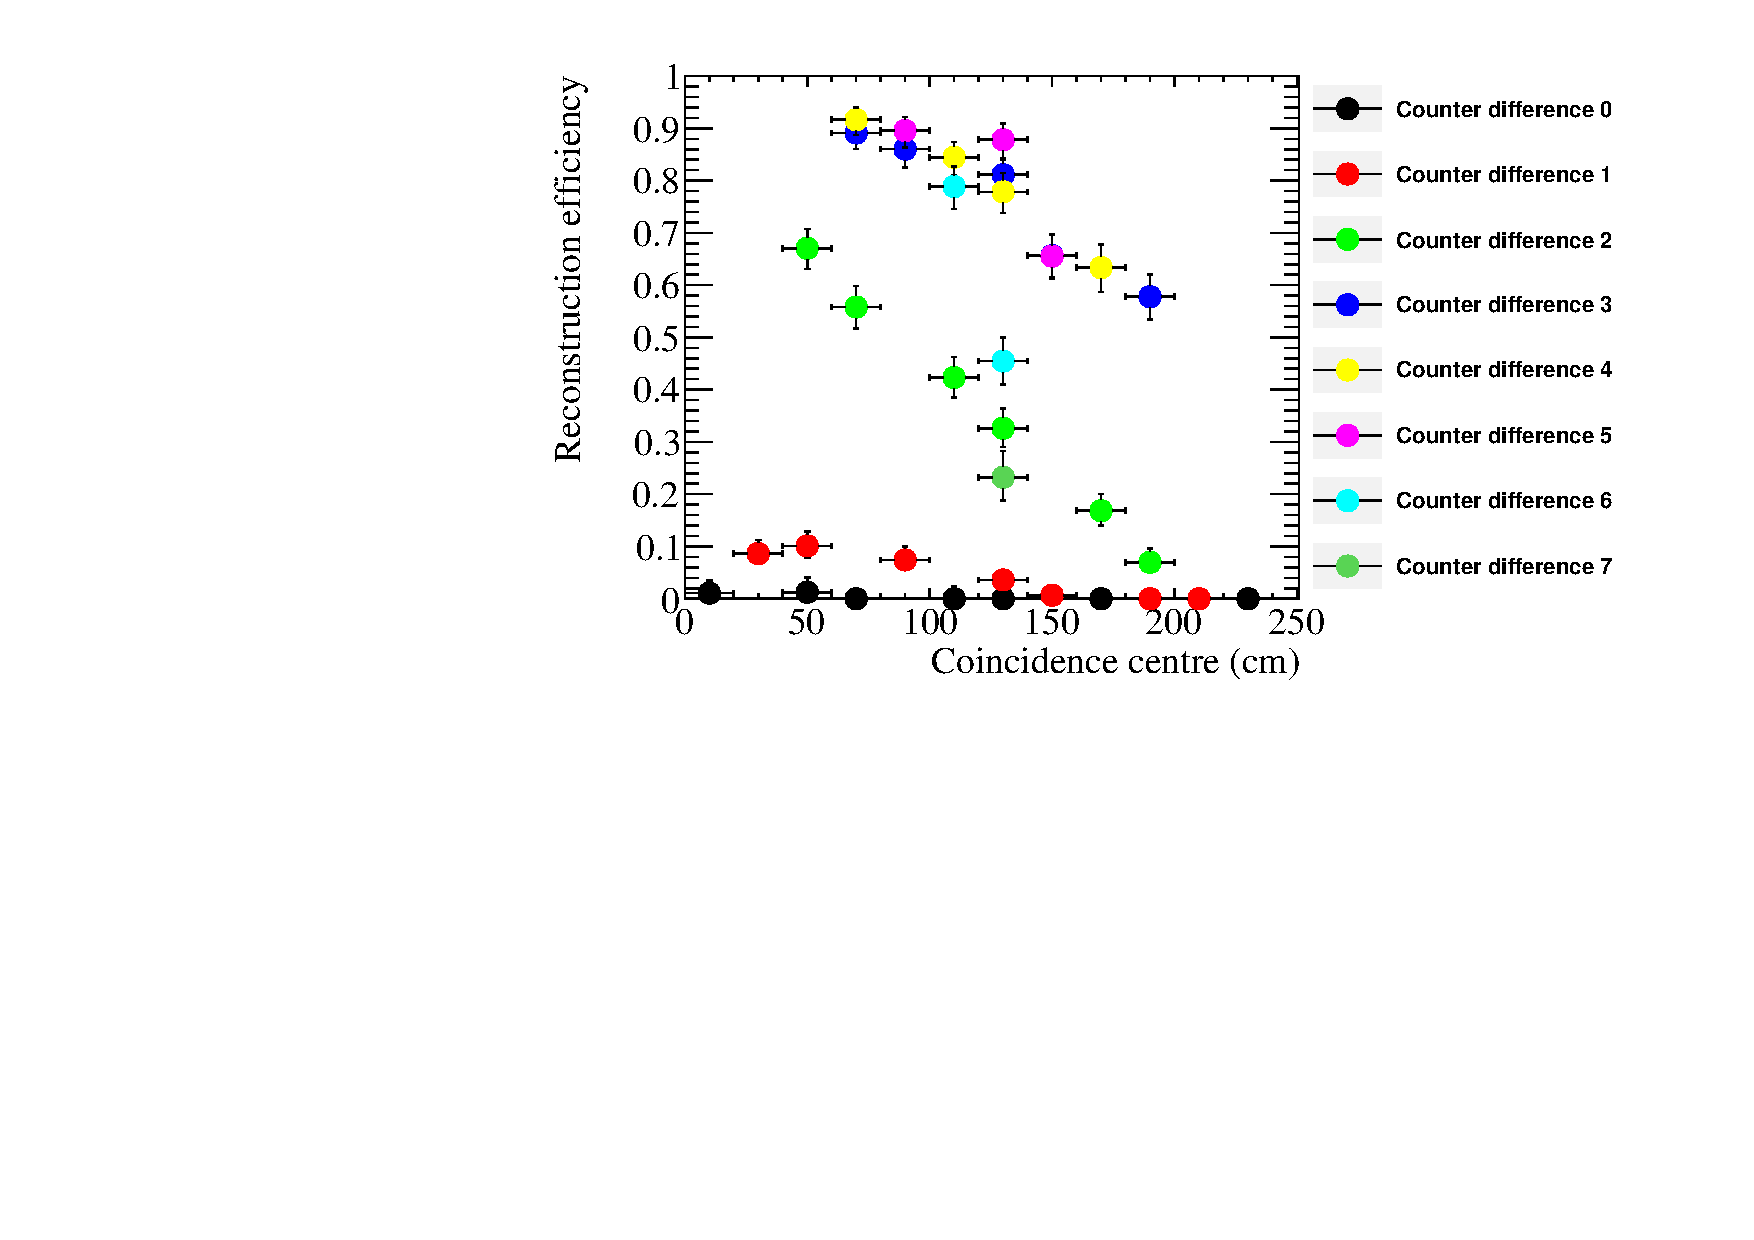
\includegraphics[width=\textwidth]{DistanceCanvas_50}
    \caption{The reconstruction efficiency as a function of coincidence centres for different counter differences.}
    \label{fig:DistanceCanvas}
  \end{subfigure}

  \begin{subfigure}{0.48\textwidth}
    \centering
    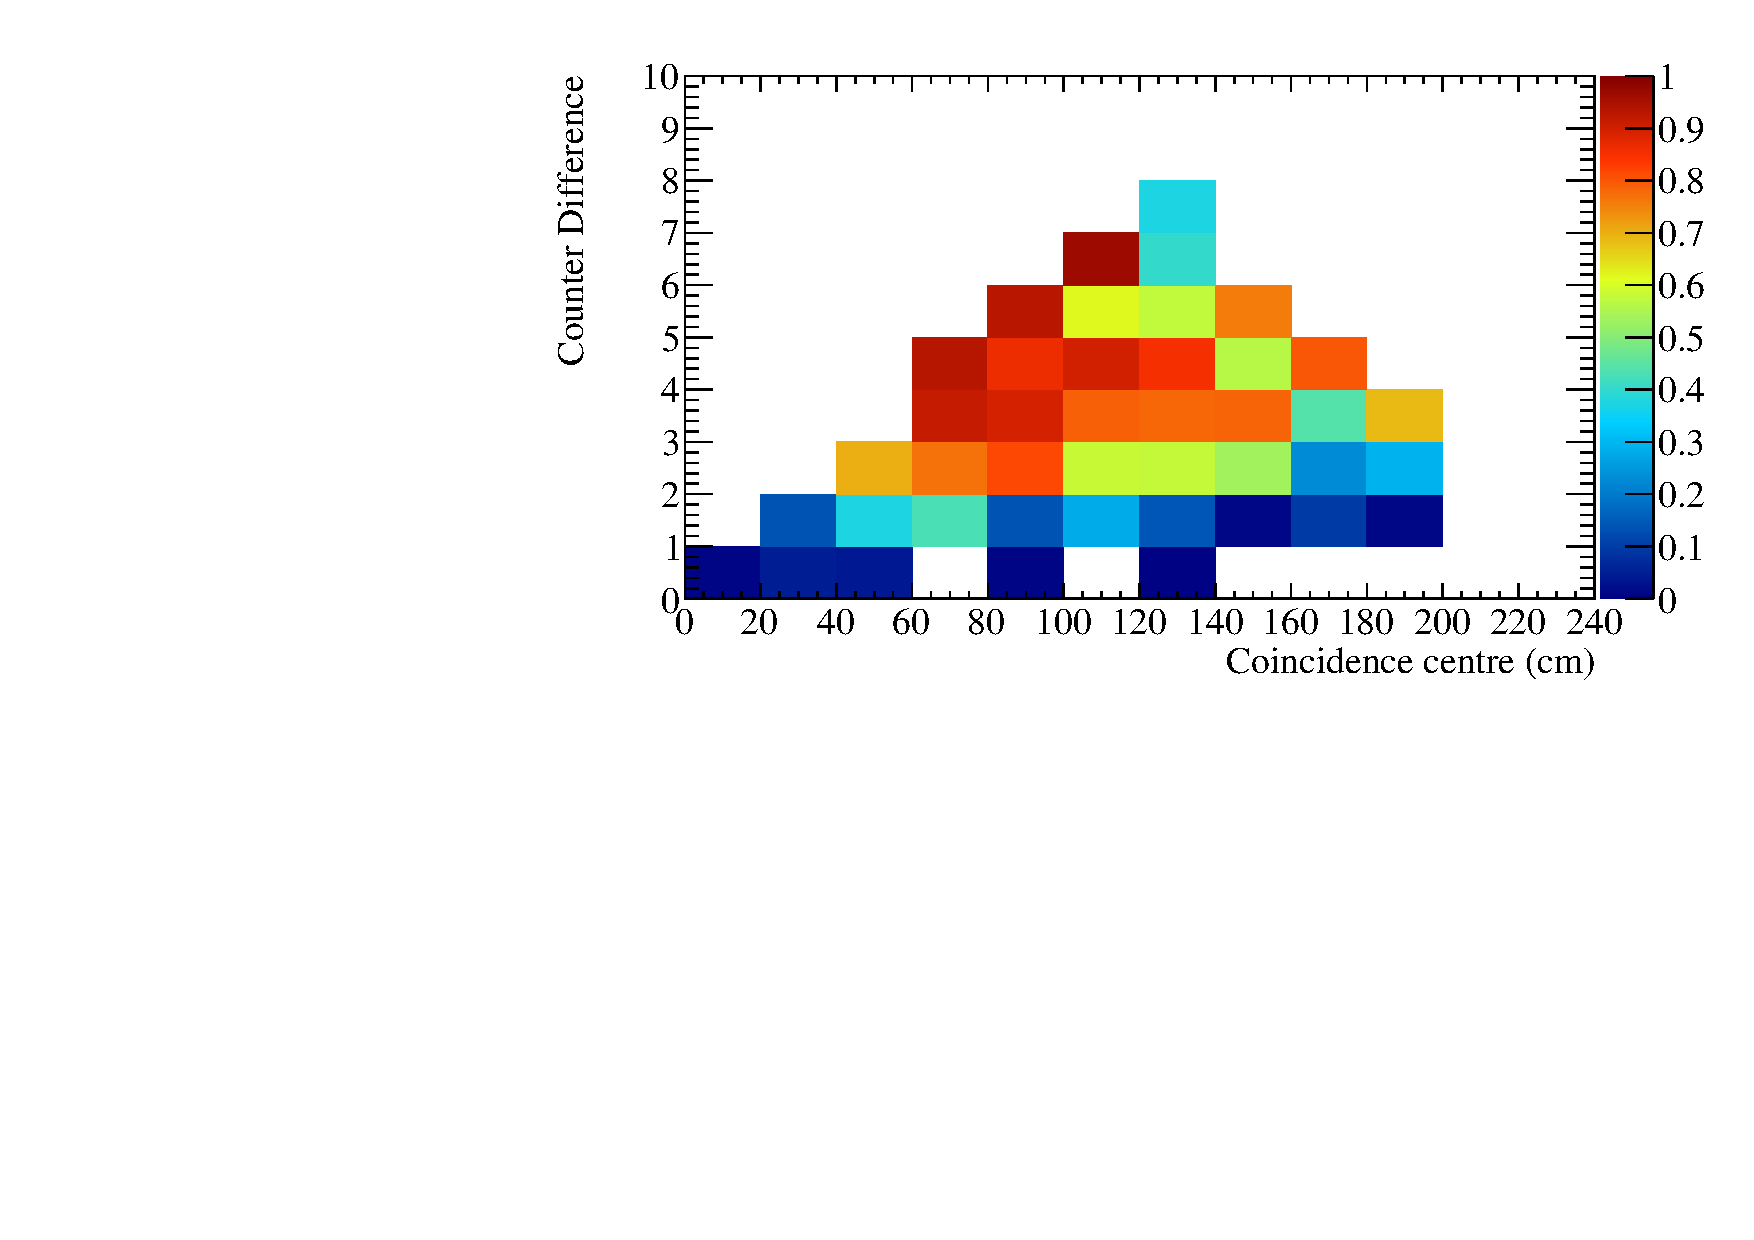
\includegraphics[width=\textwidth]{TwoDimensional_50cm}
    \caption{The reconstruction efficiency as a function of coincidence centre against the counter differences.}
    \label{fig:TwoDimCanvas}
  \end{subfigure}%
  \hspace{0.03\textwidth}%
  \begin{subfigure}{0.48\textwidth}
    \centering
    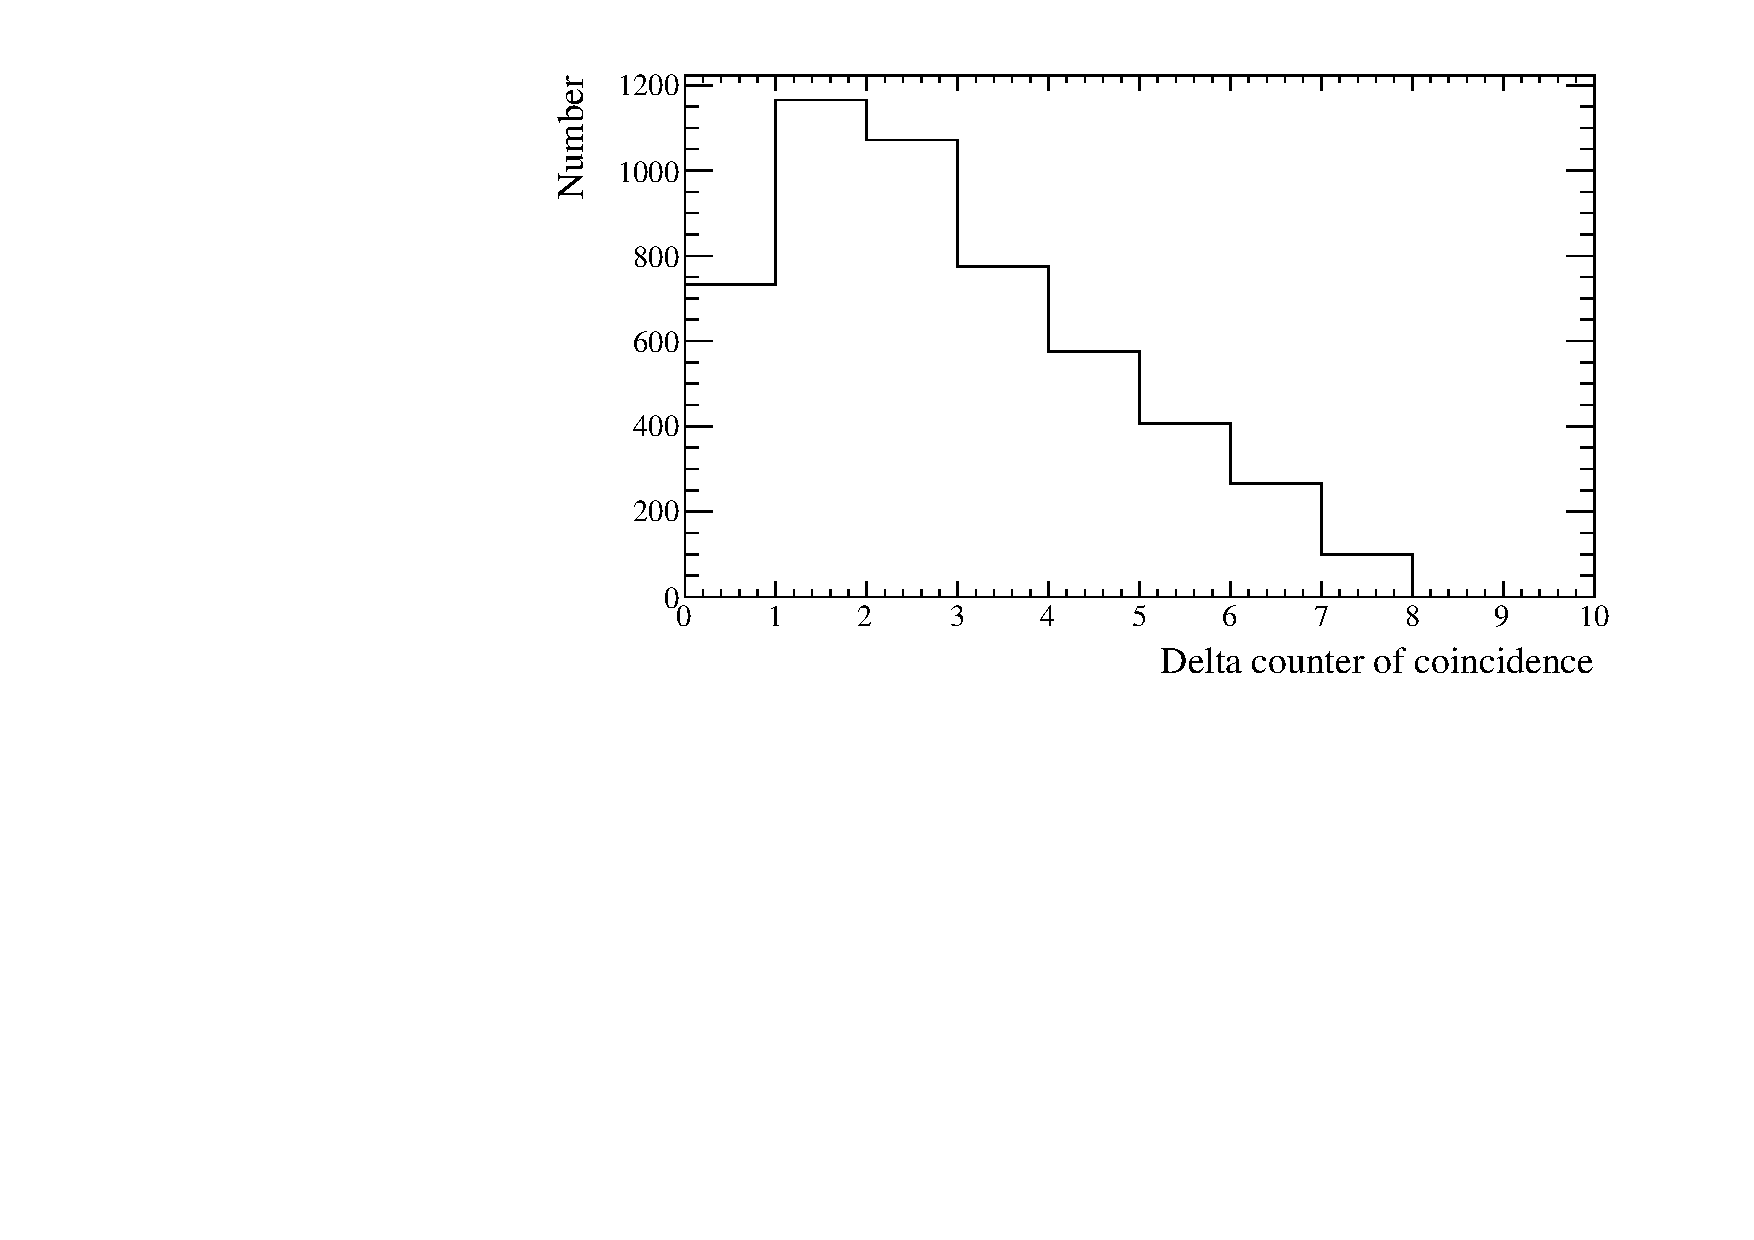
\includegraphics[width=\textwidth]{CounterDiffCan}
    \caption{The number of events for each counter difference that were recorded in the data, and the number of those which were successfully reconstructed.}
    \label{fig:CounterDiffFreq}
  \end{subfigure}
  \caption[Reconstruction efficiencies of through going tracks in the 35 ton data]
          {The reconstruction efficiencies for coincidences that trigger an east-west coincidence in the 35 ton data over a 2 day running period.}
  \label{fig:DataRecoEffics}
\end{figure}
    
From Figure~\ref{fig:AngleCanvas}, it is evident that the reconstruction efficiency for tracks with shallow angles relative to the APAs is extremely poor, with the efficiency for tracks aligned with counter differences of 0 or 1 never rising above 10\%. This is due to the coherent noise removal, where hits which are correlated in time will be removed as they will be perceived as being due to the coherent noise, as opposed to being due to real signals. As the difference in counter number increases, the efficiency is seen to increase, though the rate of this increase is seen to depend on the ``coincidence centre''. The effect of increasing ``coincidence centre'' can be seen more clearly in Figure~\ref{fig:DistanceCanvas}, where the efficiency for each counter difference as a function of ``coincidence centre'' is plotted. Here, it can be seen that the reconstruction efficiency decreases for coincidences that are centred further away from the APAs. This is due to the fact that when an energy deposition has further to drift, it will induce a smaller pulse on the wires, meaning that it is more likely to be below the hit threshold. Figure~\ref{fig:TwoDimCanvas} combines Figures~\ref{fig:AngleCanvas} and~\ref{fig:DistanceCanvas}, to show how the reconstruction efficiency for increasing ``coincidence centre'' changes, with increasing counter difference. It can be seen that tracks with counter differences of between 3 and 5, where the ``coincidence centre'' is between 60~cm and 140~cm away from the APAs, are the best reconstructed coincidences. Finally, Figure~\ref{fig:CounterDiffFreq} shows how the frequency of coincidences of a given counter difference occurs, compared to how many events contain reconstructed tracks which are aligned with the coincidence. It can be seen that, as stated earlier, the most common counter difference is 1, with the least common being a counter difference of 9. However, given the low reconstruction efficiency seen for the lowest counter differences, few tracks are reconstructed. This means that when considering the reconstructed tracks, most are due to coincidences with counter differences of either 3, 4 or 5.

%********************************** % Fifth Section  *************************************
\section{Measuring interaction times using electron diffusion}  \label{sec:DiffusionAnalysis}%Section - X.5
As electrons drift from the interaction point to the wire planes they become spread out in both time and space, this effect is known as diffusion, and is an important property of electron transport in LAr, which must be well understood. The mechanism by which diffusion occurs in LAr was first discussed in~\citep{1974NucIM.122..319D, Derenzo, PhysRevA.20.2547, Atrazhev-Timoshkin}, and has since been developed to consist of a complete set of measurements for electric fields between 100 and 2000~V$\cdot$cm$^{-1}$~\citep{Li:2015rqa}. The diffusion of electrons is rarely isotropic, and so the component that is transverse to the drift field, and the component that is parallel to the drift field, are normally measured separately. Diffusion parallel to the drift field is called longitudinal diffusion, and is generally smaller than the component of diffusion that is transverse to the drift field. Figure~\ref{fig:DomDiffSchem} shows how diffusion can smear the electrons collected on a set of wires when the electrons are initially highly correlated in time and space. \\

\begin{figure}
  \centering
  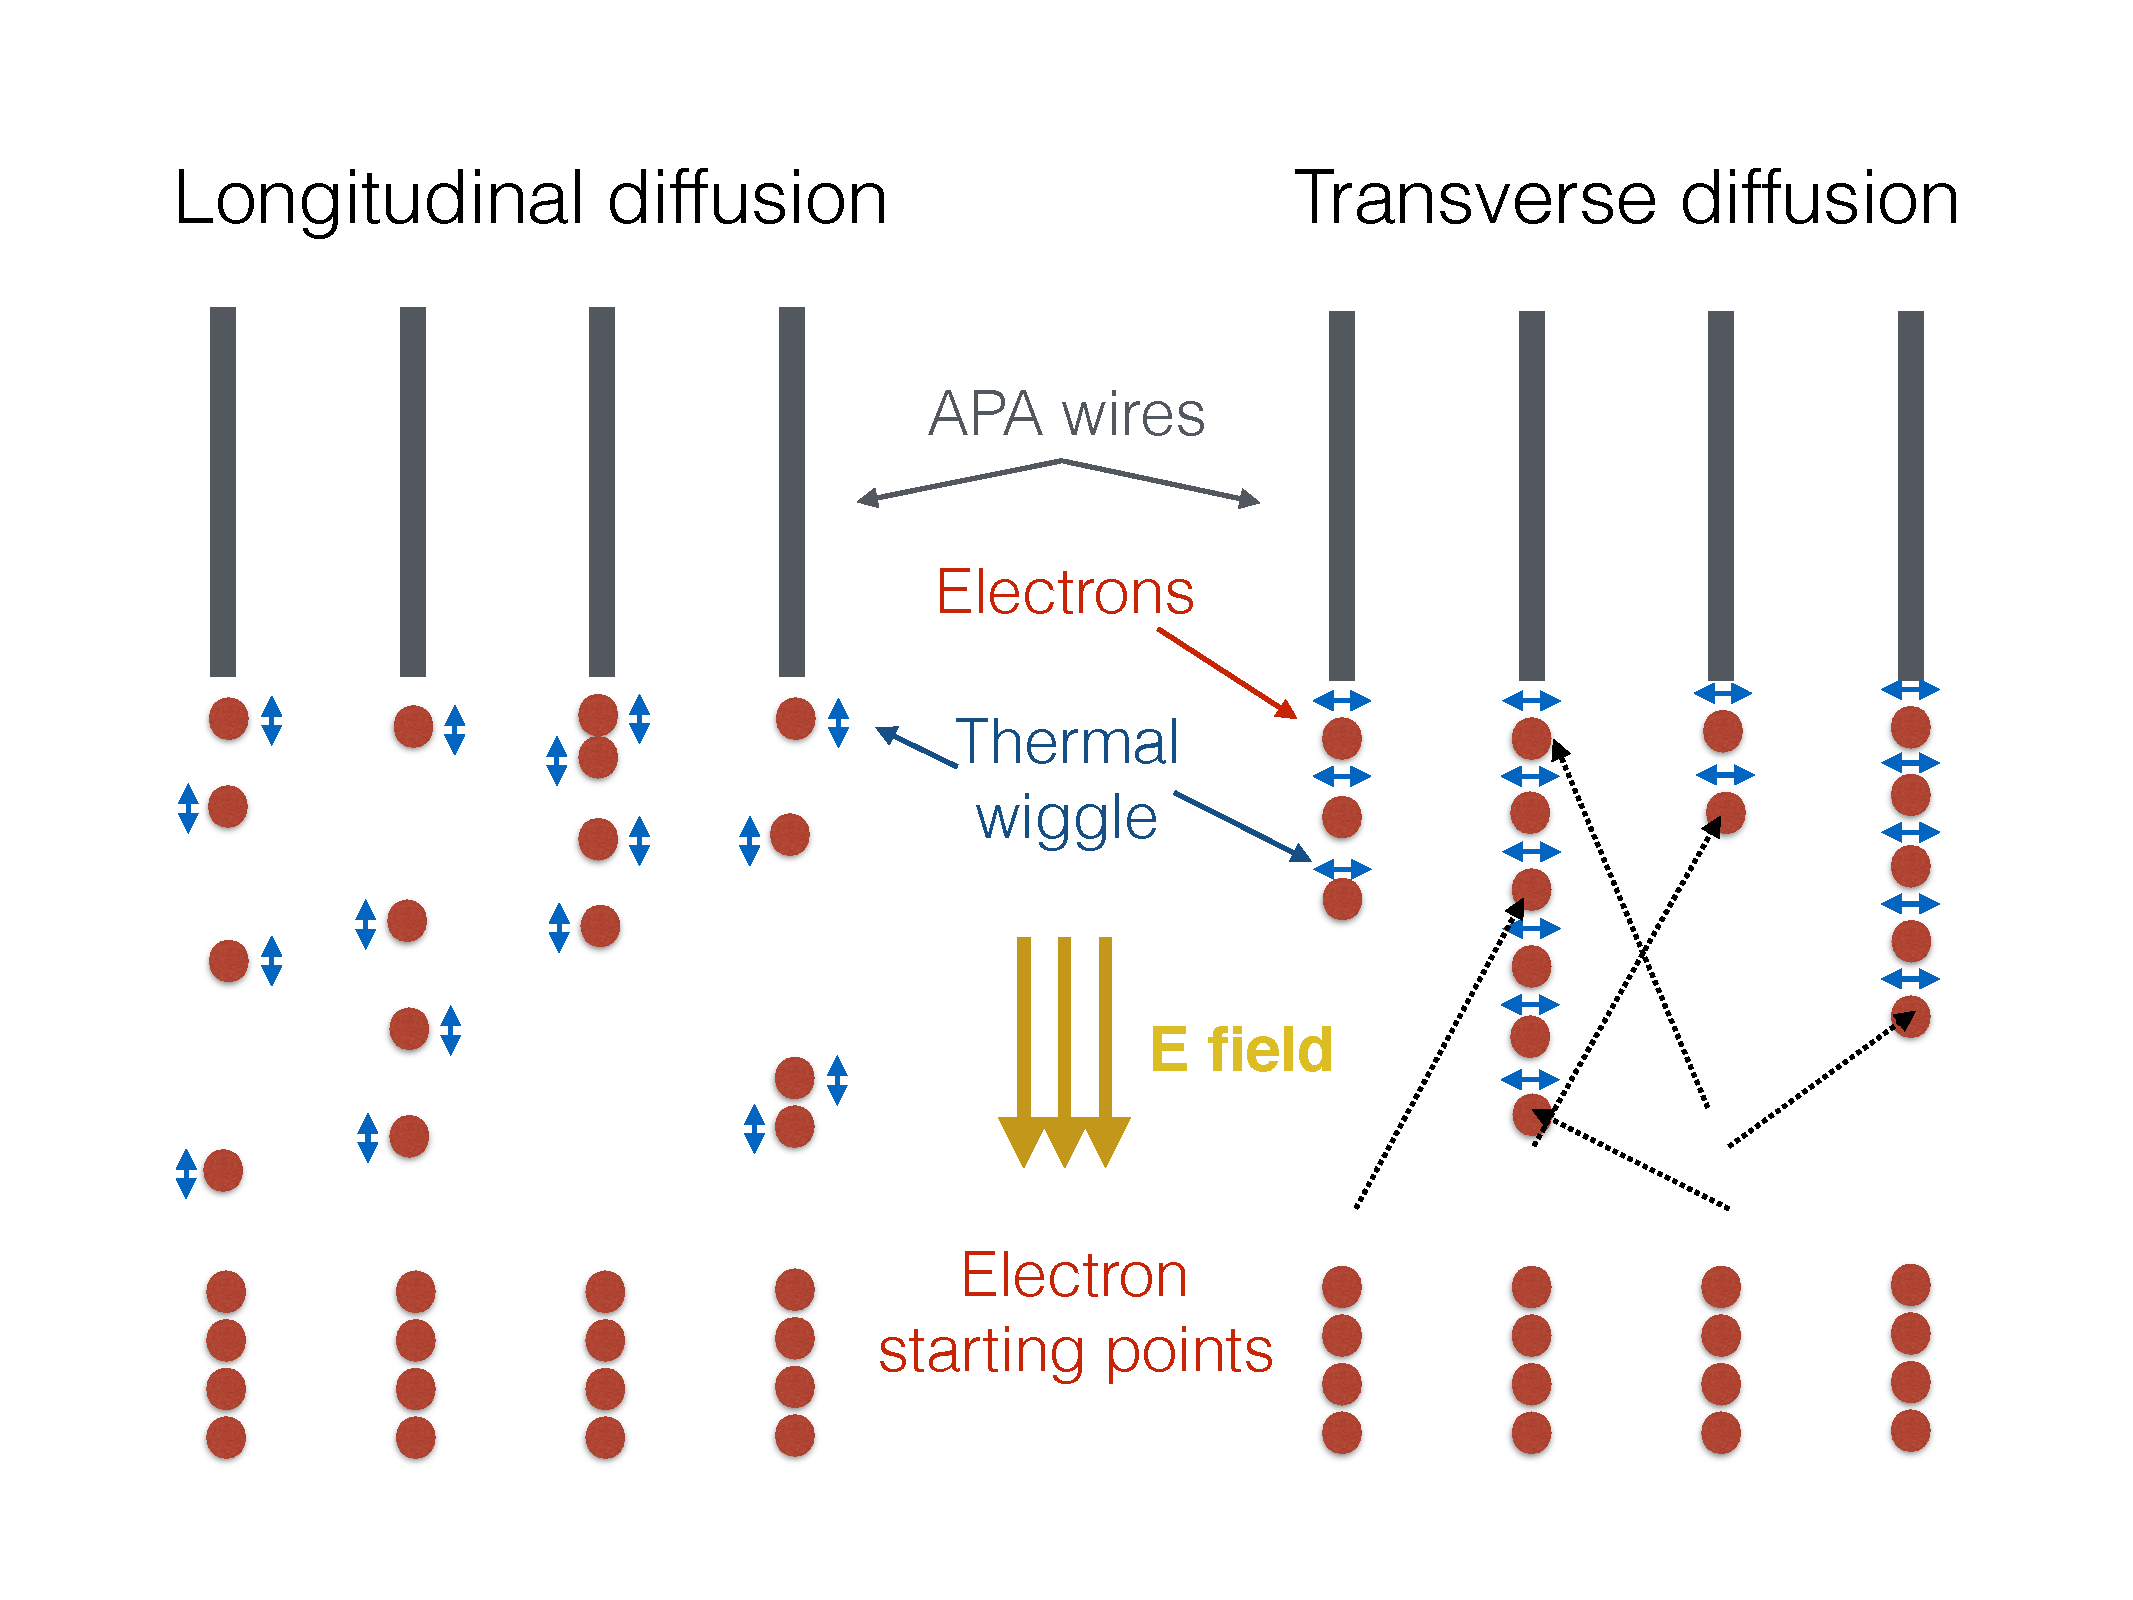
\includegraphics[width=0.85\textwidth]{DiffusionSchematic}
  \caption[Schematic showing the process of diffusion]
          {A schematic showing the longitudinal diffusion (left), and the transverse diffusion (right), of electrons. In both cases, four electrons are initially shown below four wires, and are allowed to diffuse in either the drift direction, or perpendicular to the drift direction, in the longitudinal and transverse cases respectively. It can be seen that the effect of longitudinal diffusion is to make the electrons spread out in time, whilst the effect of transverse diffusion is to make the electrons spread out in space. The figure is taken from~\citep{DomSeptMeeting}.}
  \label{fig:DomDiffSchem}
\end{figure}

Longitudinal diffusion has the effect of spreading the drifting electrons out in time, causing signals to become wider in time, and smaller in height, as the total charge is conserved. The increasing hit width can be measured for increasing drift times (distances), provided the hits do not fall below a hit finding threshold. Transverse diffusion causes drifting electrons to spread out in space, changing the amount of charge deposited on a wire, and reducing the charge resolution of the detector. Transverse diffusion is measured by discerning how the width of the hit charge distribution changes for increasing drift distances~\citep{Li:2015rqa}. \\

Through-going particles make ideal tracks to study diffusion as they are minimally ionising, and so have roughly constant energy depositions along their tracks. The tracks that they produce can also cover a wide range of drift distances, if they are not parallel to the APAs. The drift distances of hits within a track can be determined by matching the track with a counter coincidence as discussed at the end of Section~\ref{sec:DataAlgs}. The $x$ positions of the hits can then be corrected using the result of Equation~\ref{eq:HitTime_Int}, in Equation~\ref{eq:HitTime}. \\

Traditionally the only way to determine an interaction time for a track is to either match it to an external calibration source, such as whether it aligns with an external counter coincidence, or to match it to a flash of scintillation light, as in Section~\ref{sec:SimInteractionTimes}. These techniques are particularly crucial for neutrino detectors on the Earths surface, such as MicroBooNE, where each neutrino interaction usually has a background of at least one cosmic muon. The reconstructed tracks from this muon background have to be distinguished from those due to the neutrino interactions, in order correctly assign a scintillation flash to the reconstructed tracks. Figure~\ref{fig:DiffLotsOfFlashes} shows an event where scintillation flashes and cosmic muons need to be distinguished. However, it may be possible that the change in hit width due to diffusion as a particle travels through the detector could be used to determine the interaction time; though this has not been attempted before. To study whether this is possible, the effects of diffusion would have to be measured for a sample of tracks with known interaction times and orientations. \\

\begin{figure}
  \centering
  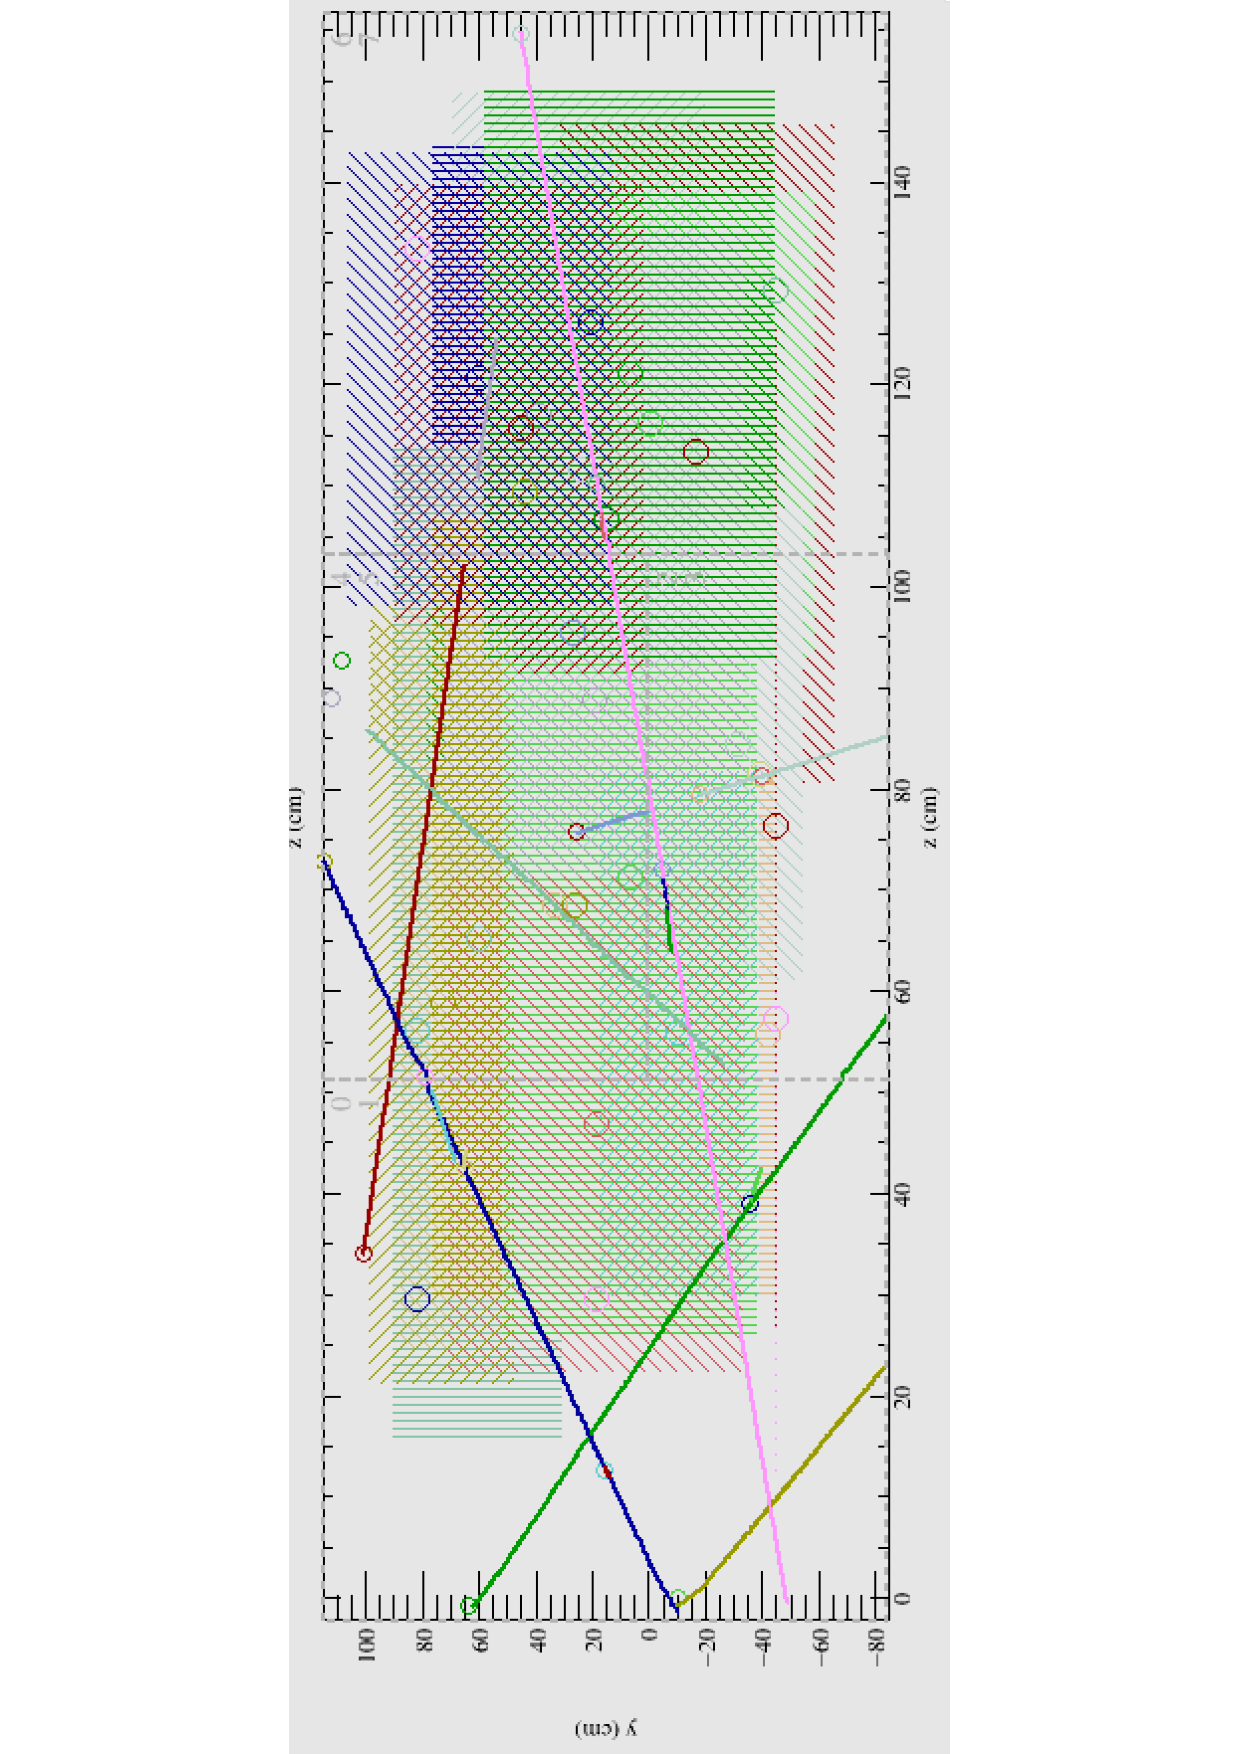
\includegraphics[width=0.95\textwidth]{LotsOfTrackFlash}
  \caption[A simulated event display showing multiple tracks and flashes in the 35 ton detector]
          {A simulated event display showing multiple tracks and flashes to be assigned to each other in the 35 ton detector, in the $yz$ plane. The coloured lines represent reconstructed tracks, whilst the coloured dashed boxes represent flashes.}
          \label{fig:DiffLotsOfFlashes}
\end{figure}

The 35 ton dataset is ideal for testing this hypothesis, as the counters are able to provide a sample of tracks with known angles and interaction times, which can be used to tune interaction time determination metrics. These metrics can then be applied to another sample of tracks, where the interaction time is known but not used, so that the accuracy of the calculated interaction times can be found. As longitudinal diffusion is the dominant effect that increases the hit width, transverse diffusion will not be directly considered further. The noise level in the 35 ton data causes reconstruction issues, and so it is also useful to compare the method against a low noise detector. Monte Carlo can provide this sample, and this comparison is shown in Section~\ref{sec:MCDataComp}. It is also useful to observe the effects that different detector conditions such as, the electric field, the electron lifetime, the noise level, and the rate of diffusion, have on the method. This is shown in Section~\ref{sec:DiffMCStudies}. First though, the method is performed on the 35 ton dataset.

%********************************** % Fifth.First Section  *************************************
\subsection{Determining interaction times in 35 ton data}
When calculating the determination metrics, only hits on wires which are not noisy are considered. This is because wires with a high level of correlated noise observe hits with a wider RMS. This is shown in Figure~\ref{fig:DomsHitModel}, where, when a baseline noise of 10~ADC counts is added to a simulated hit, with a peak value of 50~ADC counts, and an RMS of 10~ticks, the width increases by over 10\%. Hits with delta rays also need to be removed, as the deposited energy will be larger and over a longer period of time than hits from the main track. This will make the RMS of the individual hit wider, and also increase the width of the charge distribution for the track. To remove these hits only hits which satisfy the following cuts are used:
\begin{itemize}
\item No hit on the same wire within 50~ticks of the hit in question. This removes delta rays.
\item No more than 10 hits on the same wire in the whole 15,000~tick data sample. This removes clearly noisy wires.
\end{itemize}
These cuts will clearly become much more restrictive as the noise level in the detector increases, but they are essential in order to produce a dataset which is not overpowered by noise. Only collection plane hits are used, as the charge resolution is better, and the signals are unipolar as opposed to bipolar, meaning that a Gaussian function can be easily fitted to the signals. Additionally, the $signal/noise$ ratio on the collection planes was much higher than on the induction planes for the 35 ton dataset, and so the hits could be much more reliably reconstructed. \\

\begin{figure}
  \centering
  \begin{subfigure}{0.48\textwidth}
    \centering
    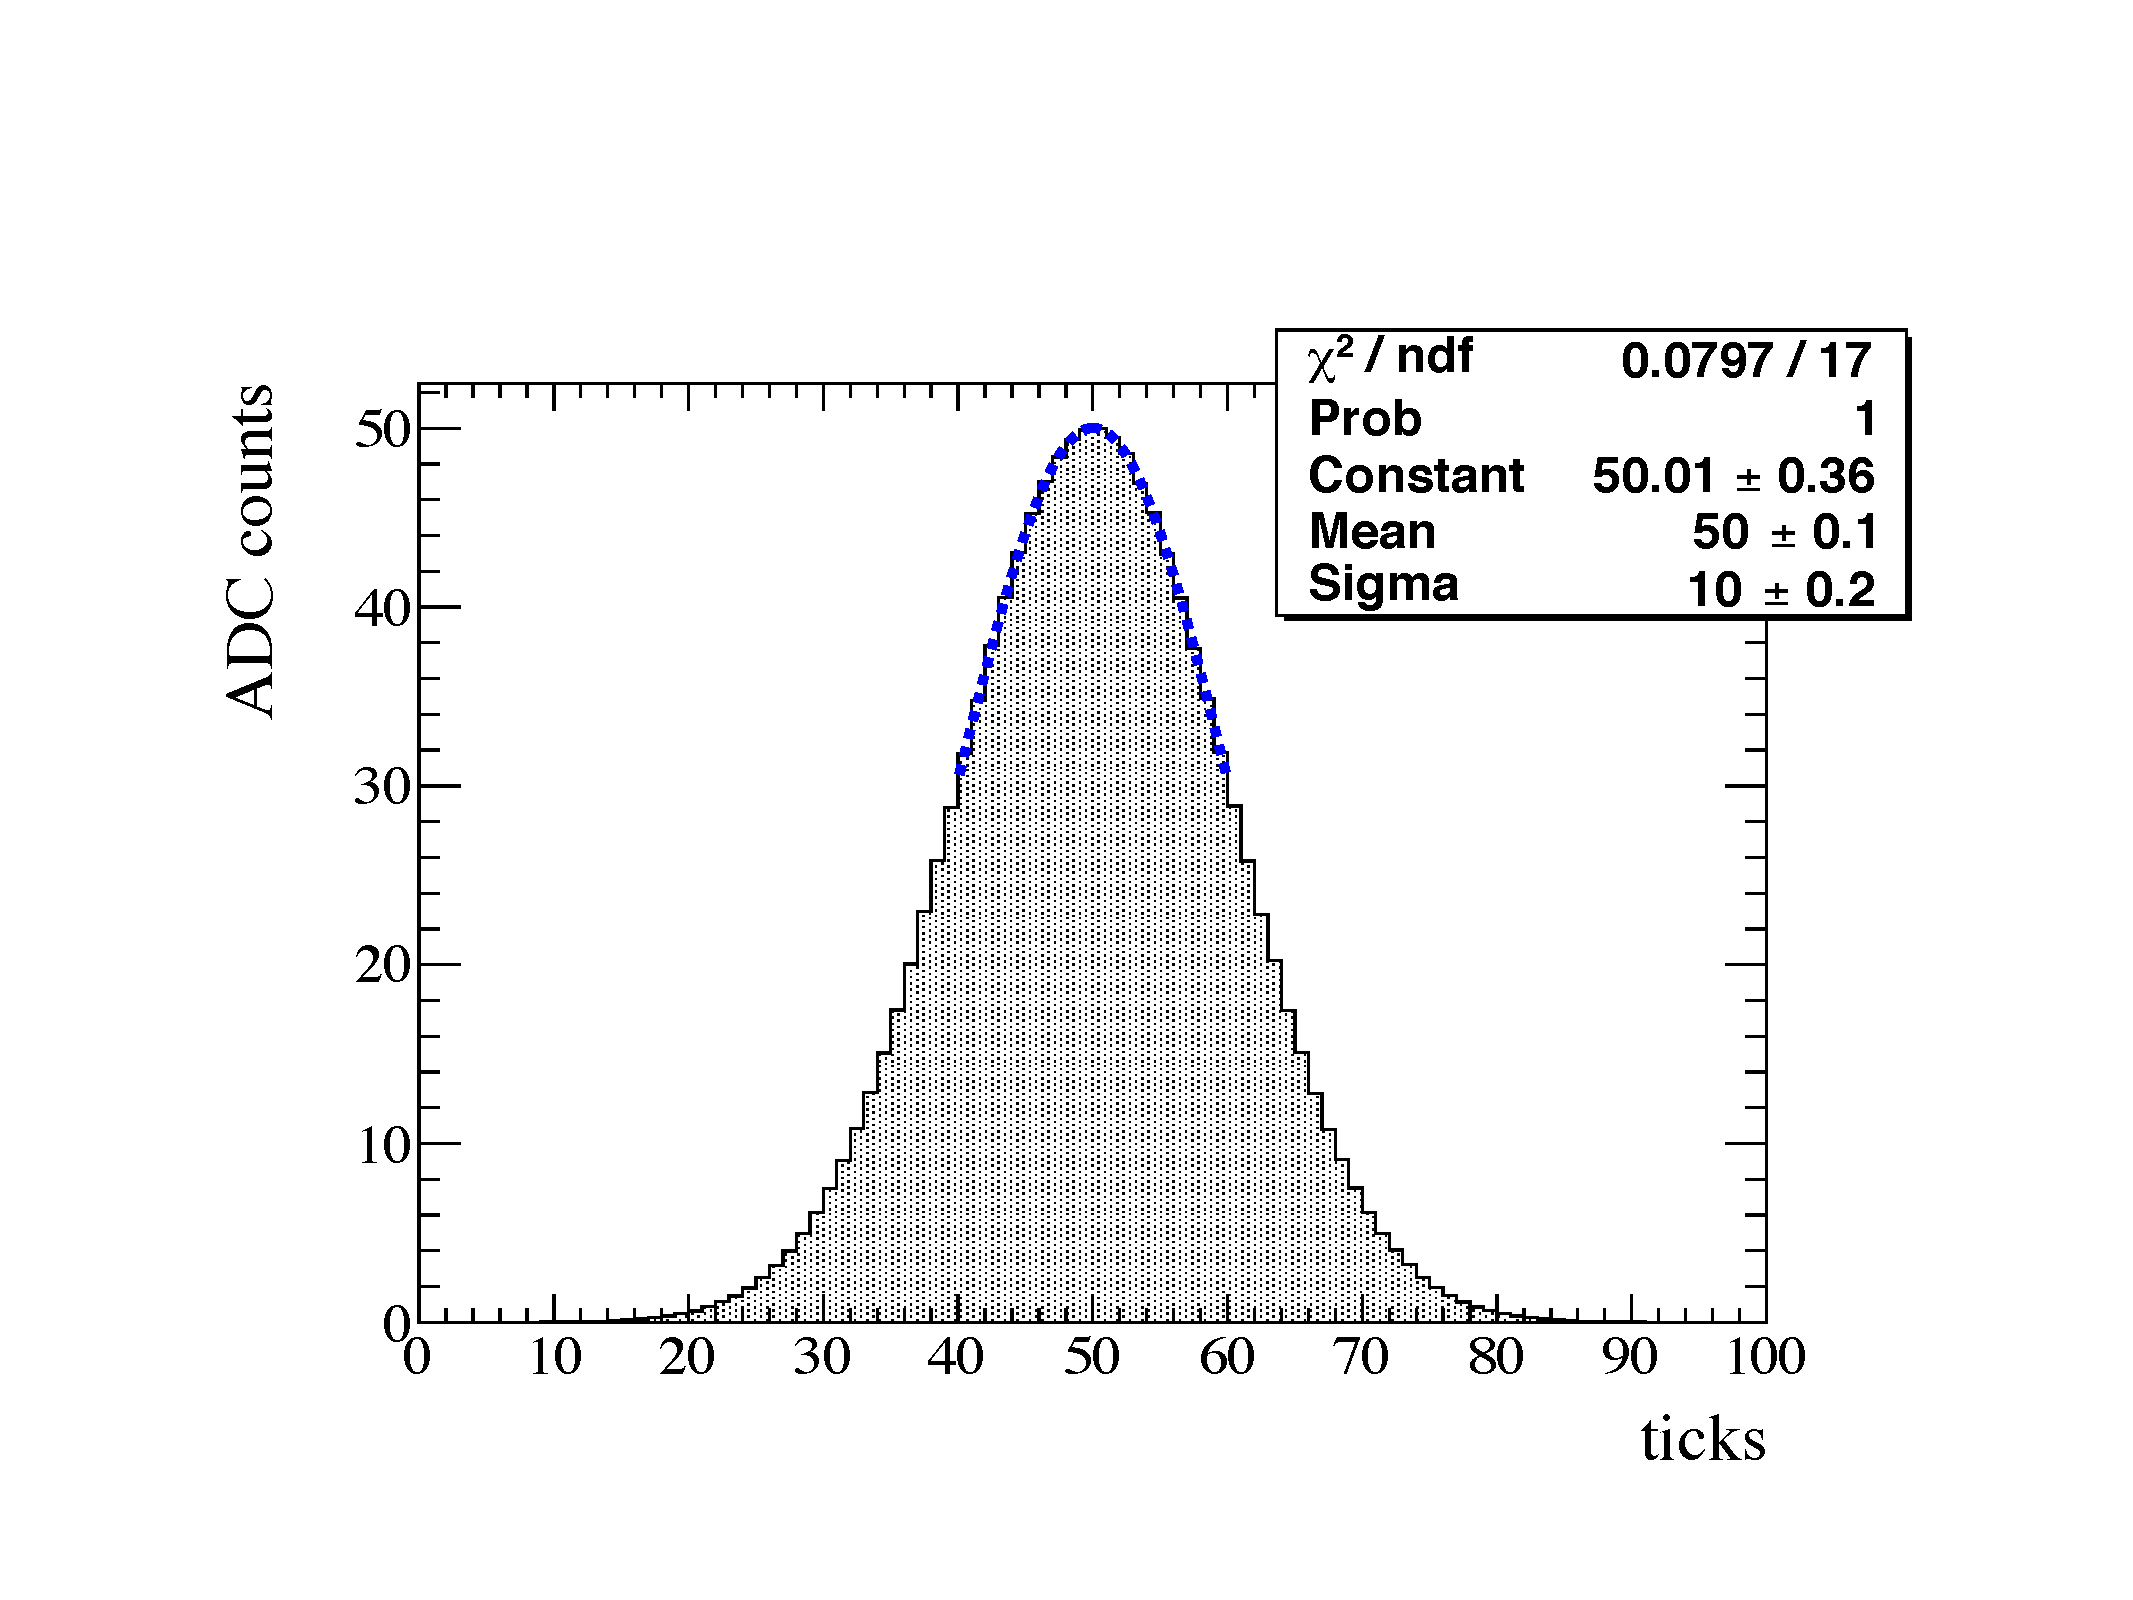
\includegraphics[width=\textwidth]{ToyGauss_Raw}
    \caption{A simulated signal.}
  \end{subfigure}%
  \hspace{0.03\textwidth}%
  \begin{subfigure}{0.48\textwidth}
    \centering
    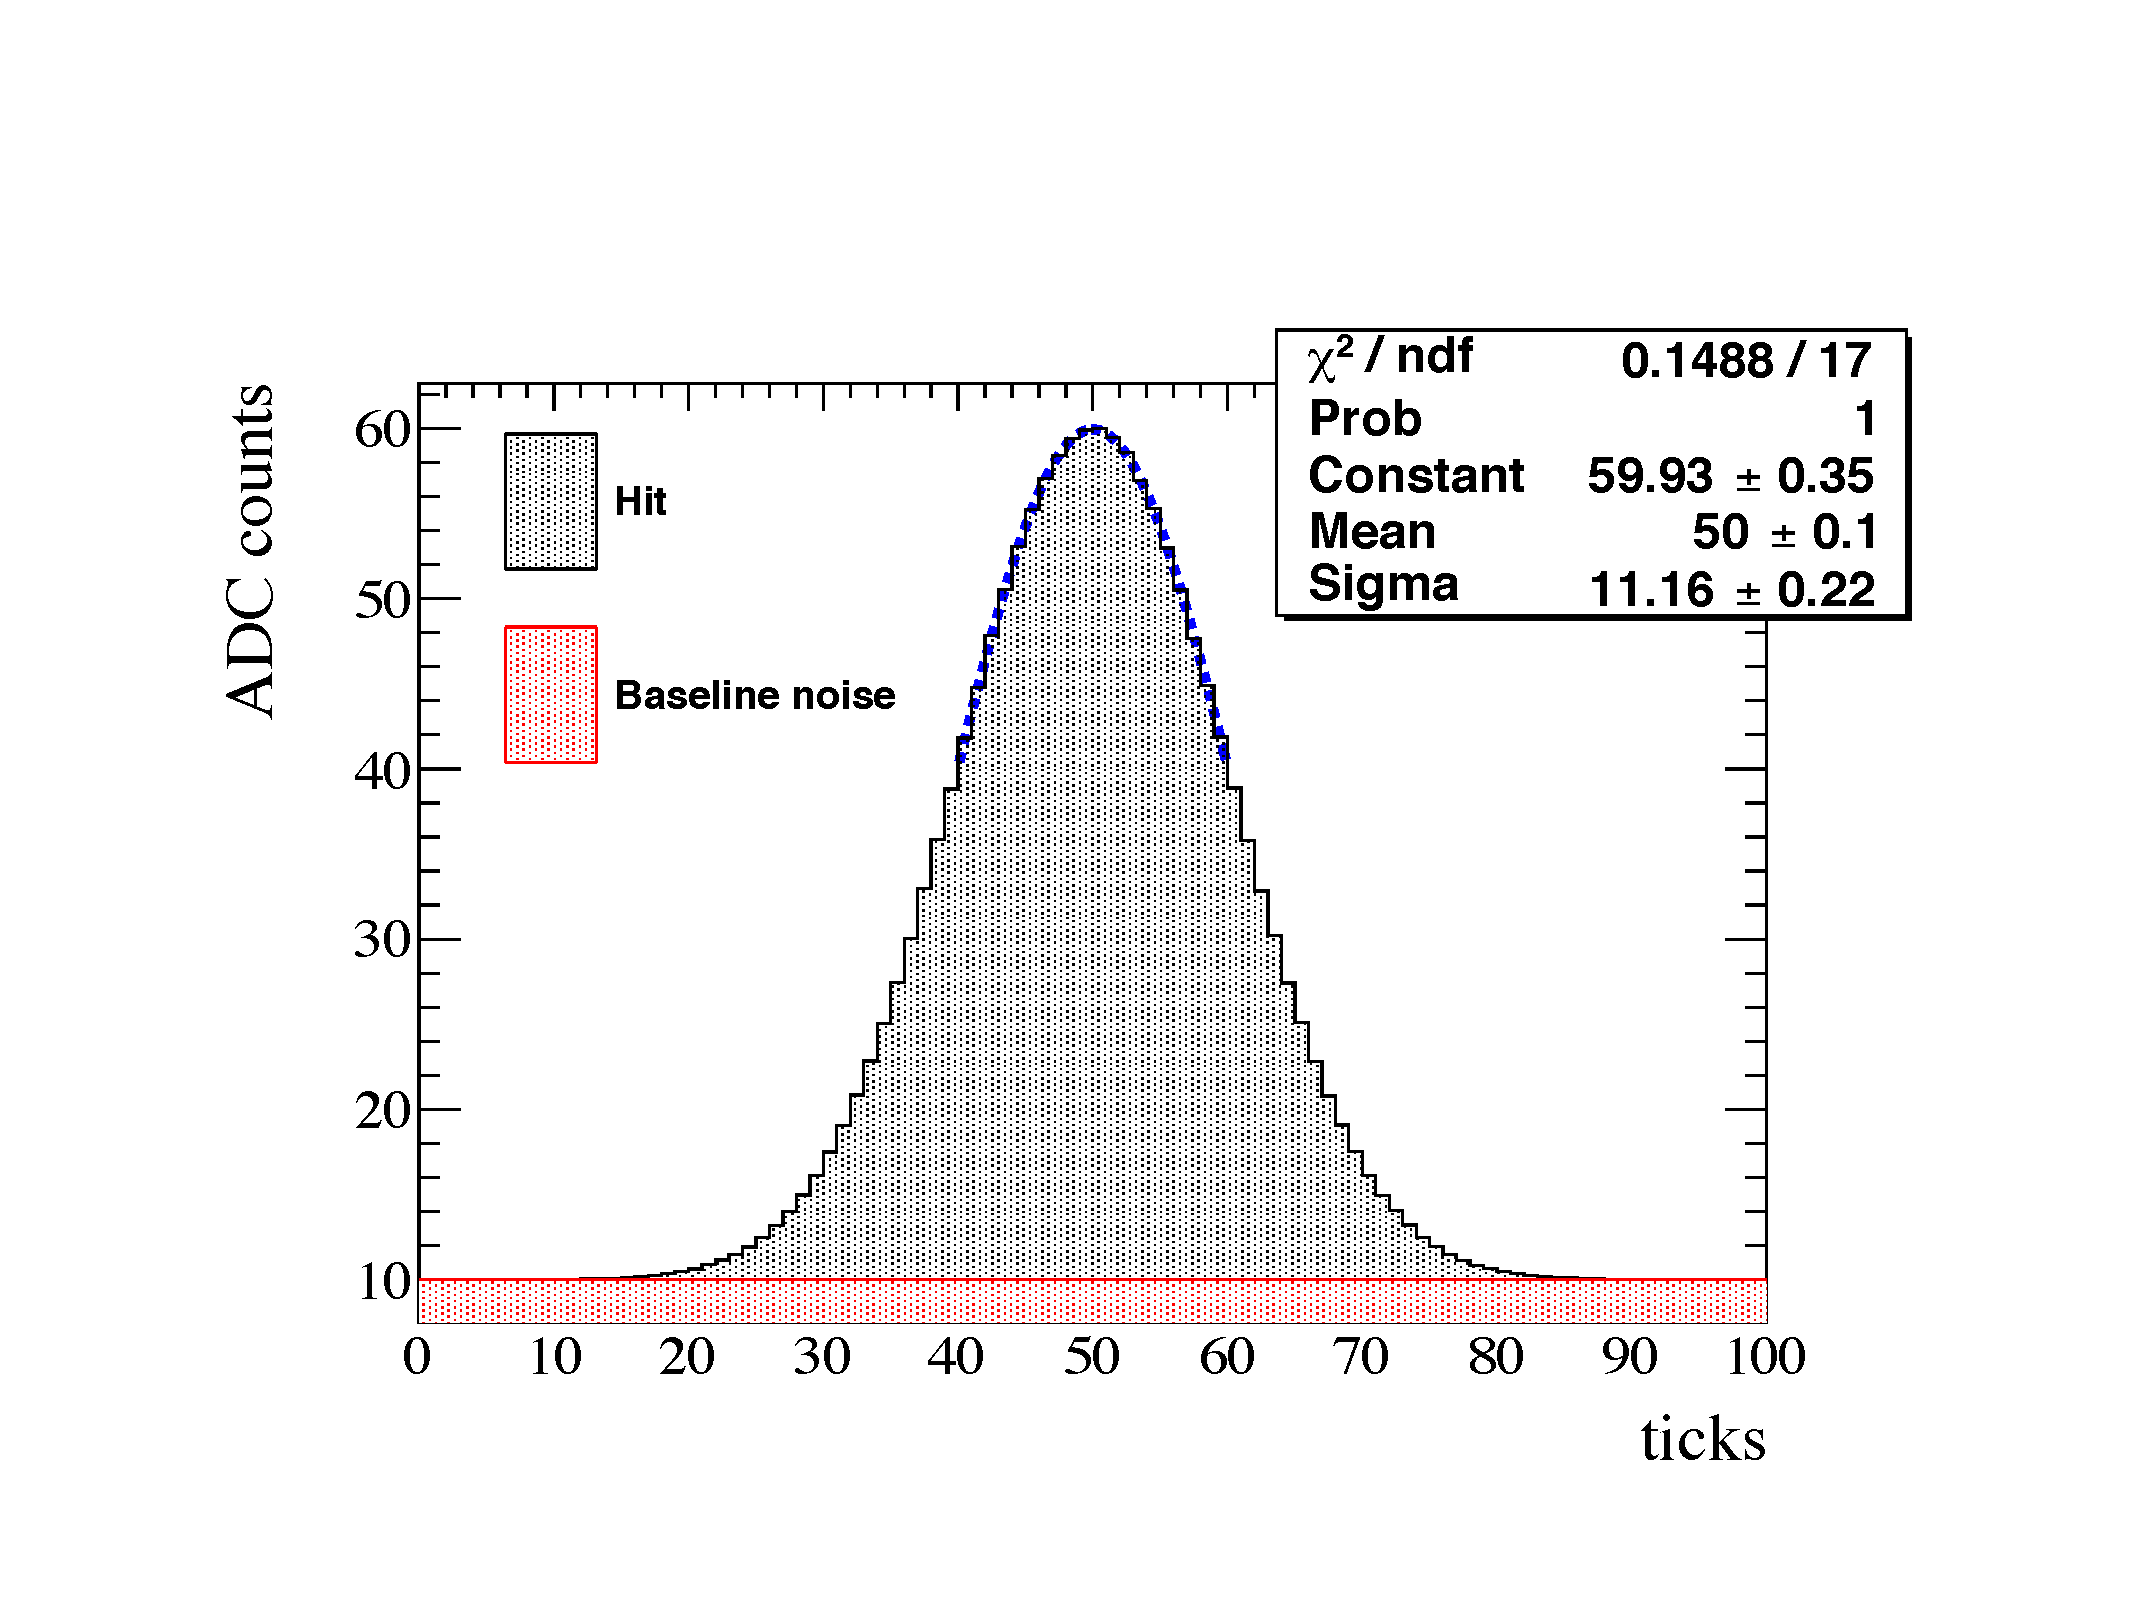
\includegraphics[width=\textwidth]{ToyGauss_Noise}
    \caption{A simulated signal with a constant noise baseline added.}
  \end{subfigure}
  \caption[The effect of adding a noise baseline to a hit]
          {ADC counts as a function of time for a simulated signal with a width of 10~ticks, and an amplitude of 50~ADC counts, both before and after, a constant noise baseline of 10~ADC counts is added. The simulated ADC value is shown on the $y$ axis, and the time, in ticks, is shown on the $x$ axis. In reality the noise would fluctuate with time. When a Gaussian function is fitted to each signal, it is seen to be more than 10\% larger for the signal where the noise baseline is added. This shows that noise can cause the measured width of a hit to increase. The figure is taken from~\citep{DomSeptMeeting}.}
          \label{fig:DomsHitModel}
\end{figure}  

Diffusion is a track angle dependent property, and so track angle ranges have to be considered independently. To minimise the number of figures presented, when graphs are made for all counter differences separately, only graphs made for tracks which have a counter difference of 4 are shown. However, the procedure for predicting interaction times is identical for tracks of all counter differences. Tracks with a counter difference of 4 were chosen as they were one of the angles for which tracks were well reconstructed in the data, see Figure~\ref{fig:DataRecoEffics}. Tracks are considered en masse, and so the hits for every track are separated into 10~cm regions of increasing drift distance from the APAs. The following quantities are calculated for each 10~cm drift region:
\begin{itemize}
\item The hit $RMS$ - the most direct way to measure transverse diffusion.
\item The hit $RMS/Charge$ - an attempt to incorporate the effect of impurities in the LAr for relatively low purity data, as this will have a drift distance dependence.
  \begin{itemize}
  \item The charge of a hit is calculated by integrating the ADCs of the reconstructed hit over time. 
  \end{itemize}
\end{itemize}
Fitting Gaussian functions around the peaks of the distributions will yield the most probable values for the drift regions, as is shown in Figure~\ref{fig:DiffDataHitFit}. \\

\begin{figure}
  \centering
  \begin{subfigure}{0.48\textwidth}
    \centering
    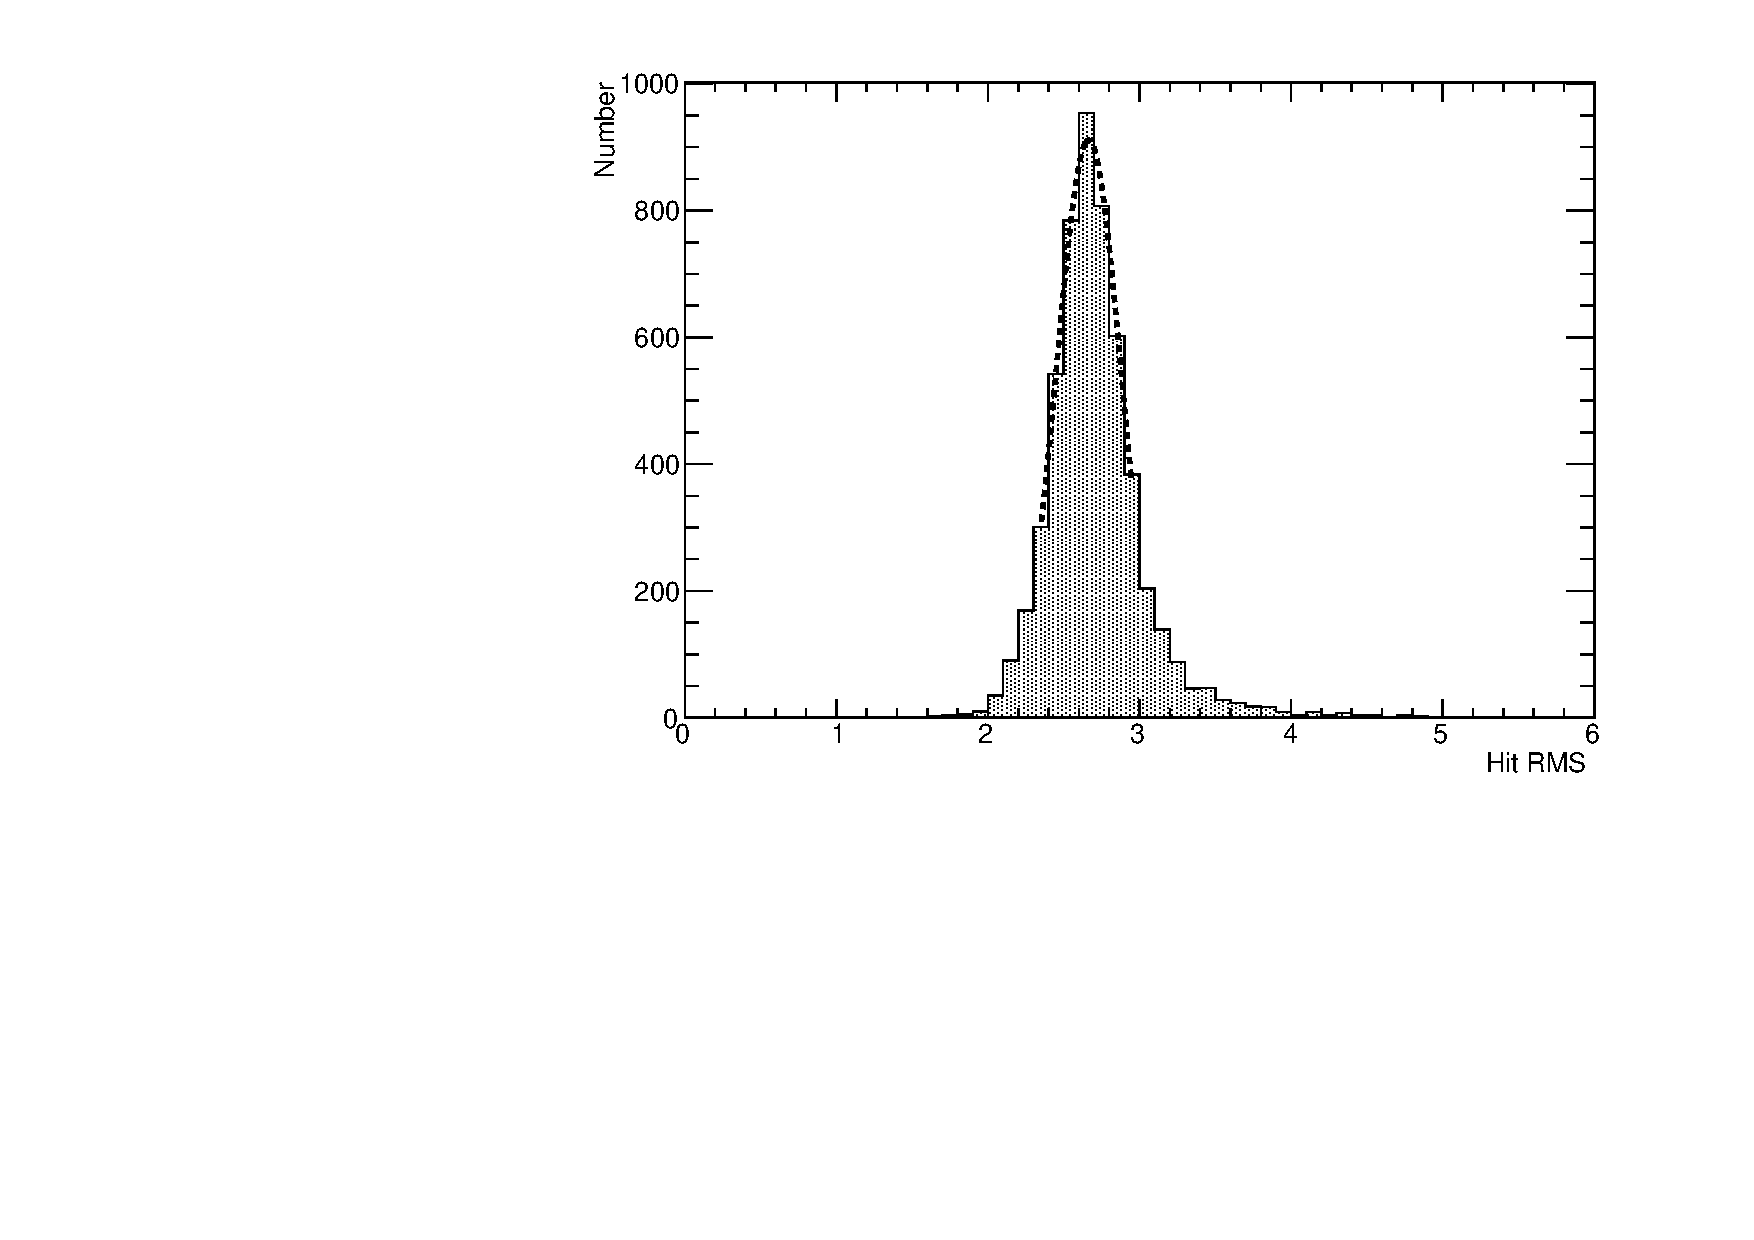
\includegraphics[width=\textwidth]{DataCan_0}
    \caption{The distribution of hit $RMS$ value for hits between $x =$ 20~cm and $x =$ 30~cm.}
  \end{subfigure}%
  \hspace{0.03\textwidth}%
  \begin{subfigure}{0.48\textwidth}
    \centering
    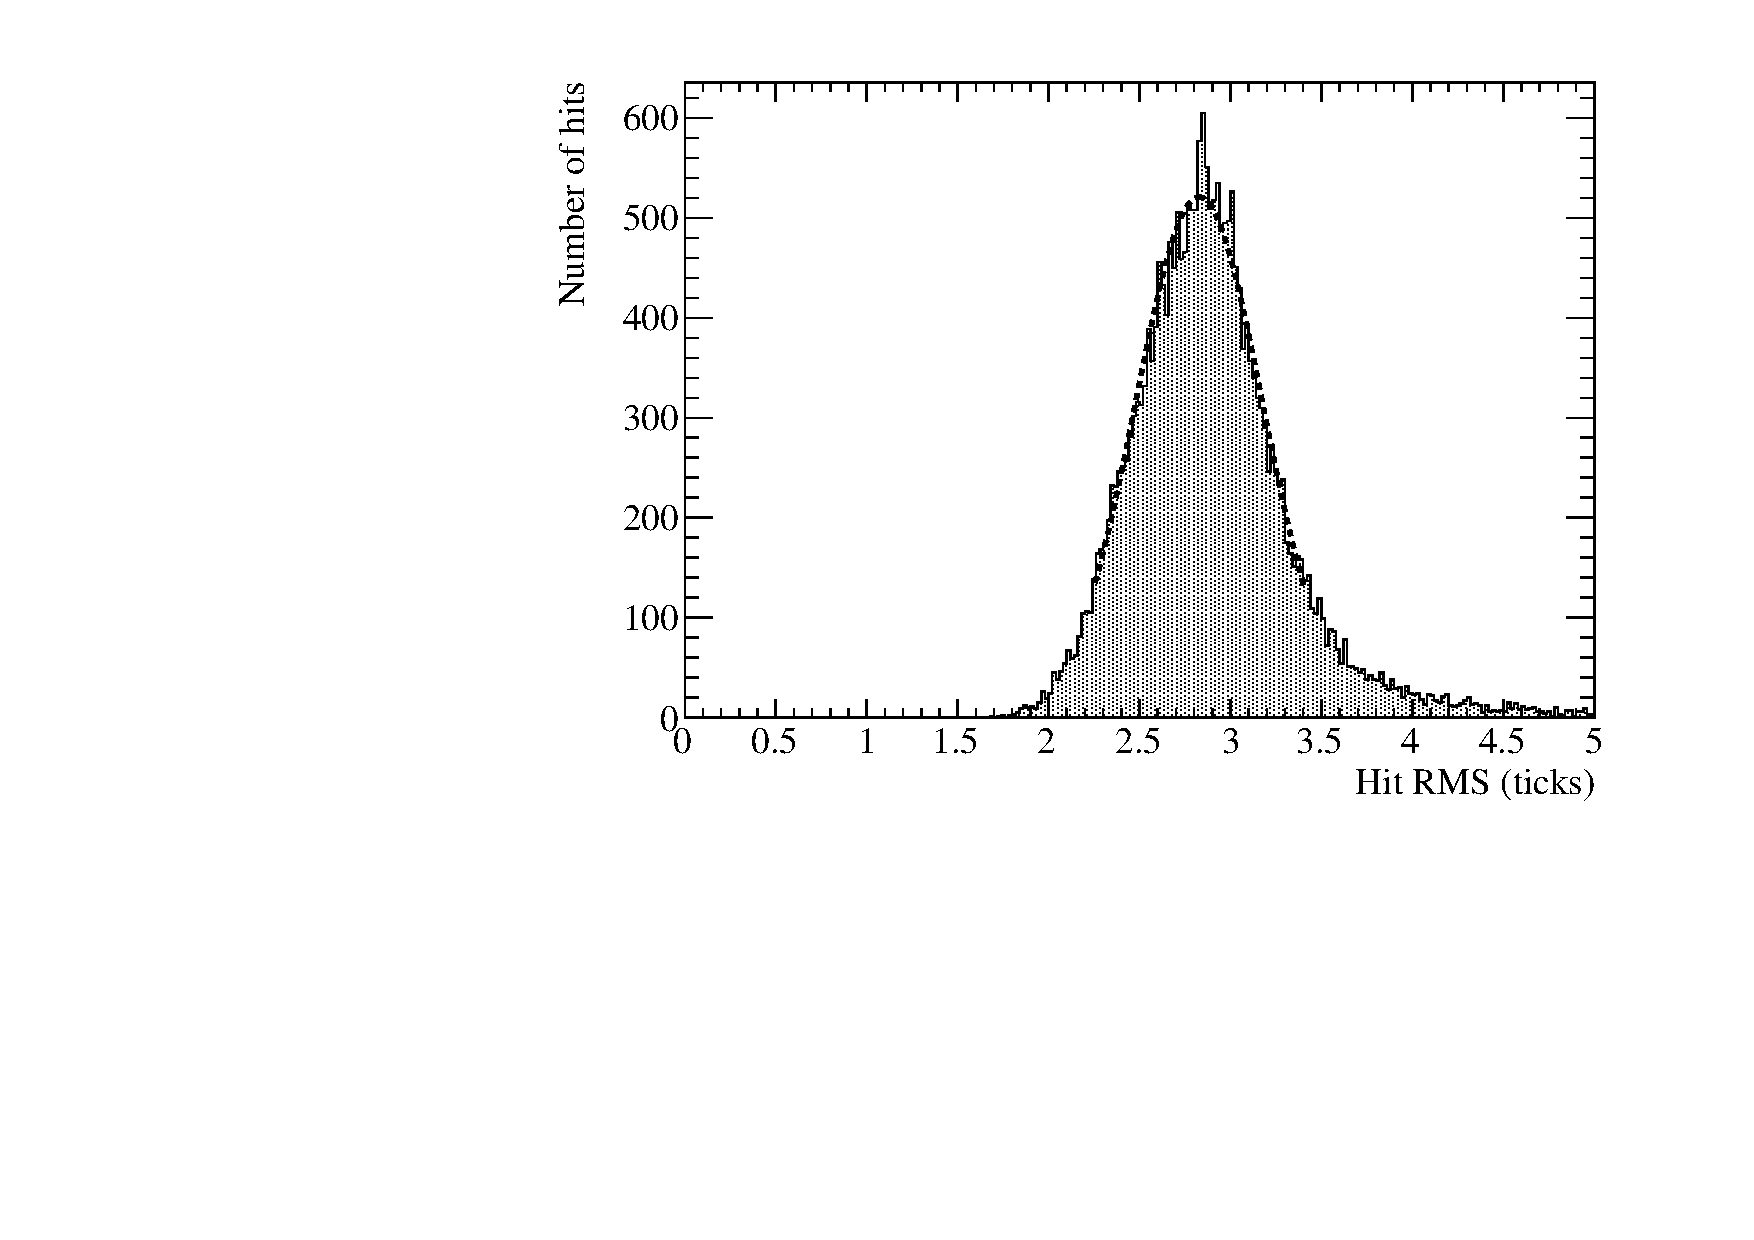
\includegraphics[width=\textwidth]{DataCan_1}
    \caption{The distribution of hit $RMS$ value for hits between $x =$ 140~cm and $x =$ 150~cm.}
  \end{subfigure}
  \begin{subfigure}{0.48\textwidth}
    \centering
    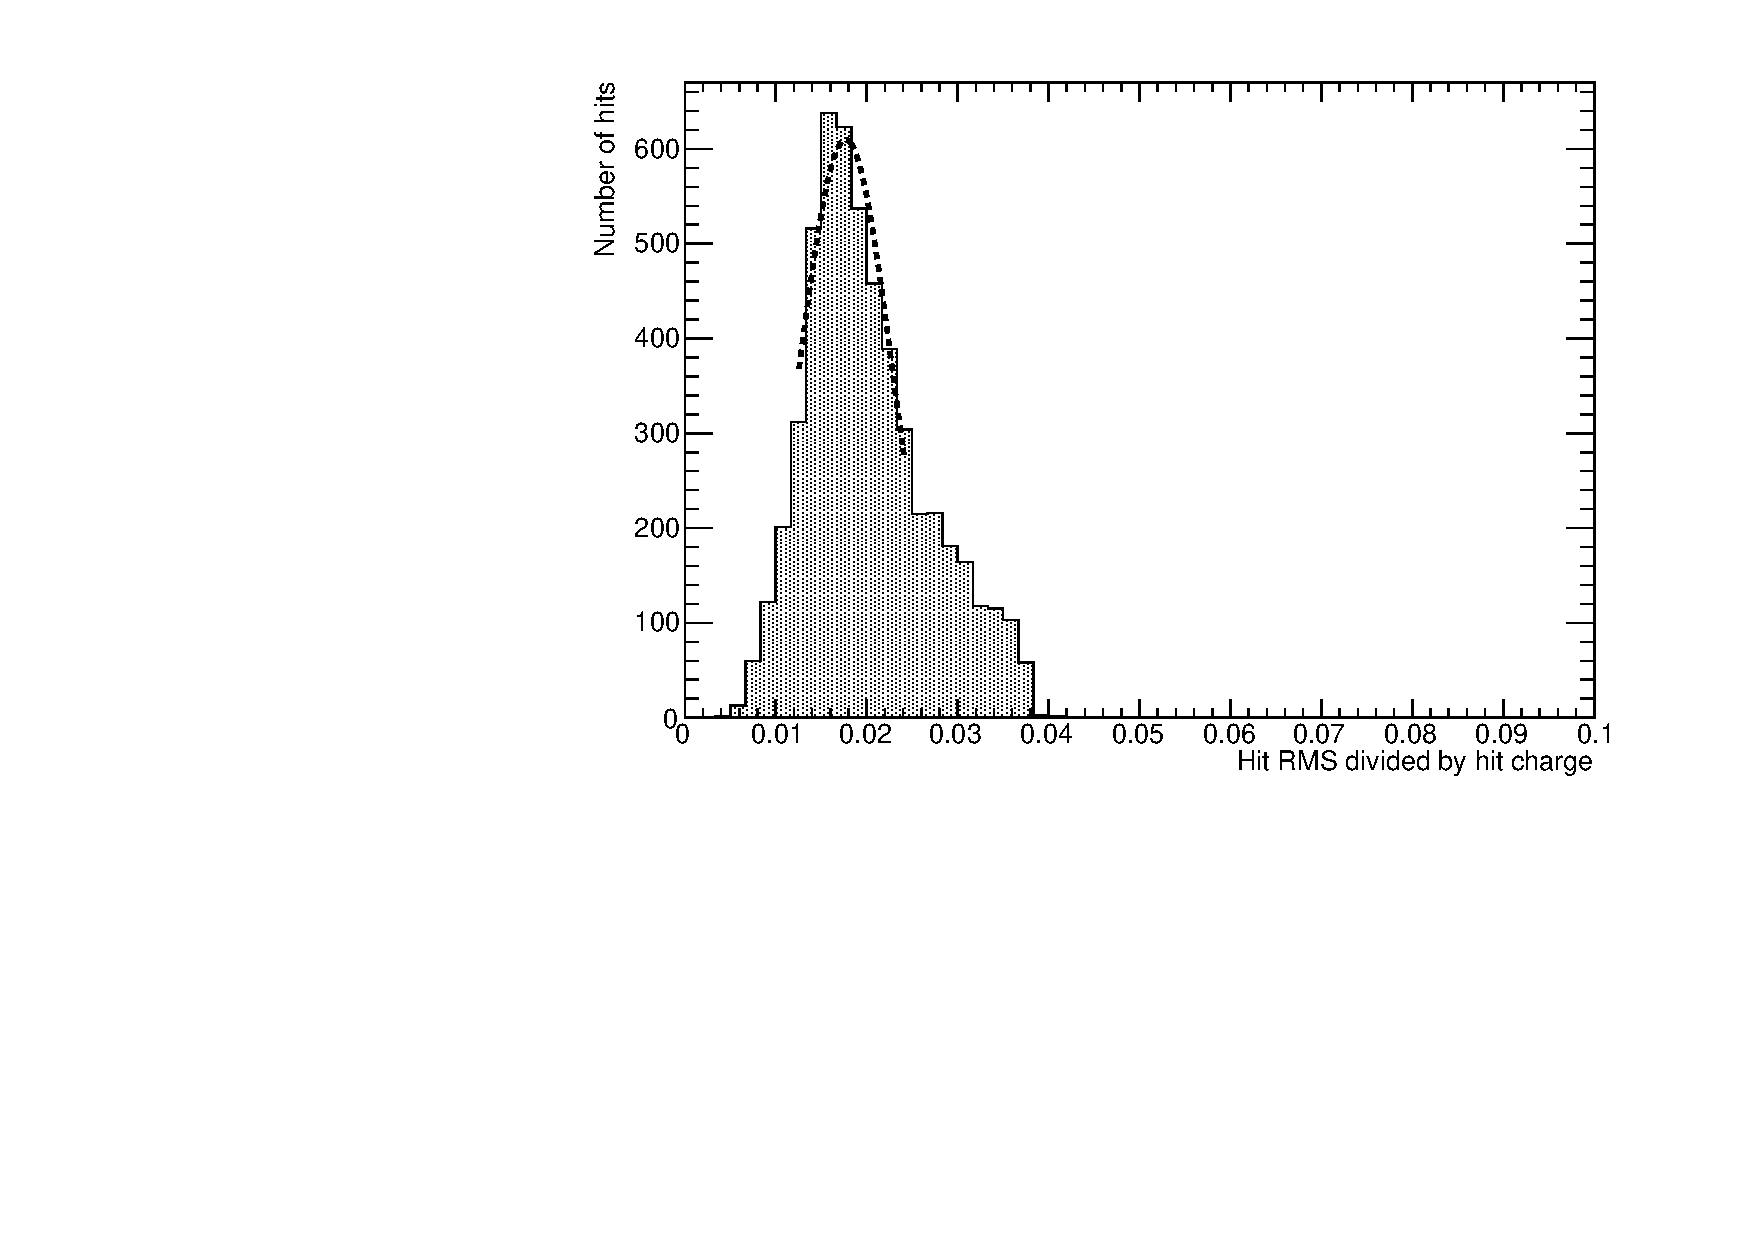
\includegraphics[width=\textwidth]{DataCan_2}
    \caption{The distribution of hit $RMS/Charge$ value for hits between $x =$ 20~cm and $x =$ 30~cm.}
    \label{fig:DiffDataHitFit_RMSQ20}
  \end{subfigure}%
  \hspace{0.03\textwidth}%
  \begin{subfigure}{0.48\textwidth}
    \centering
    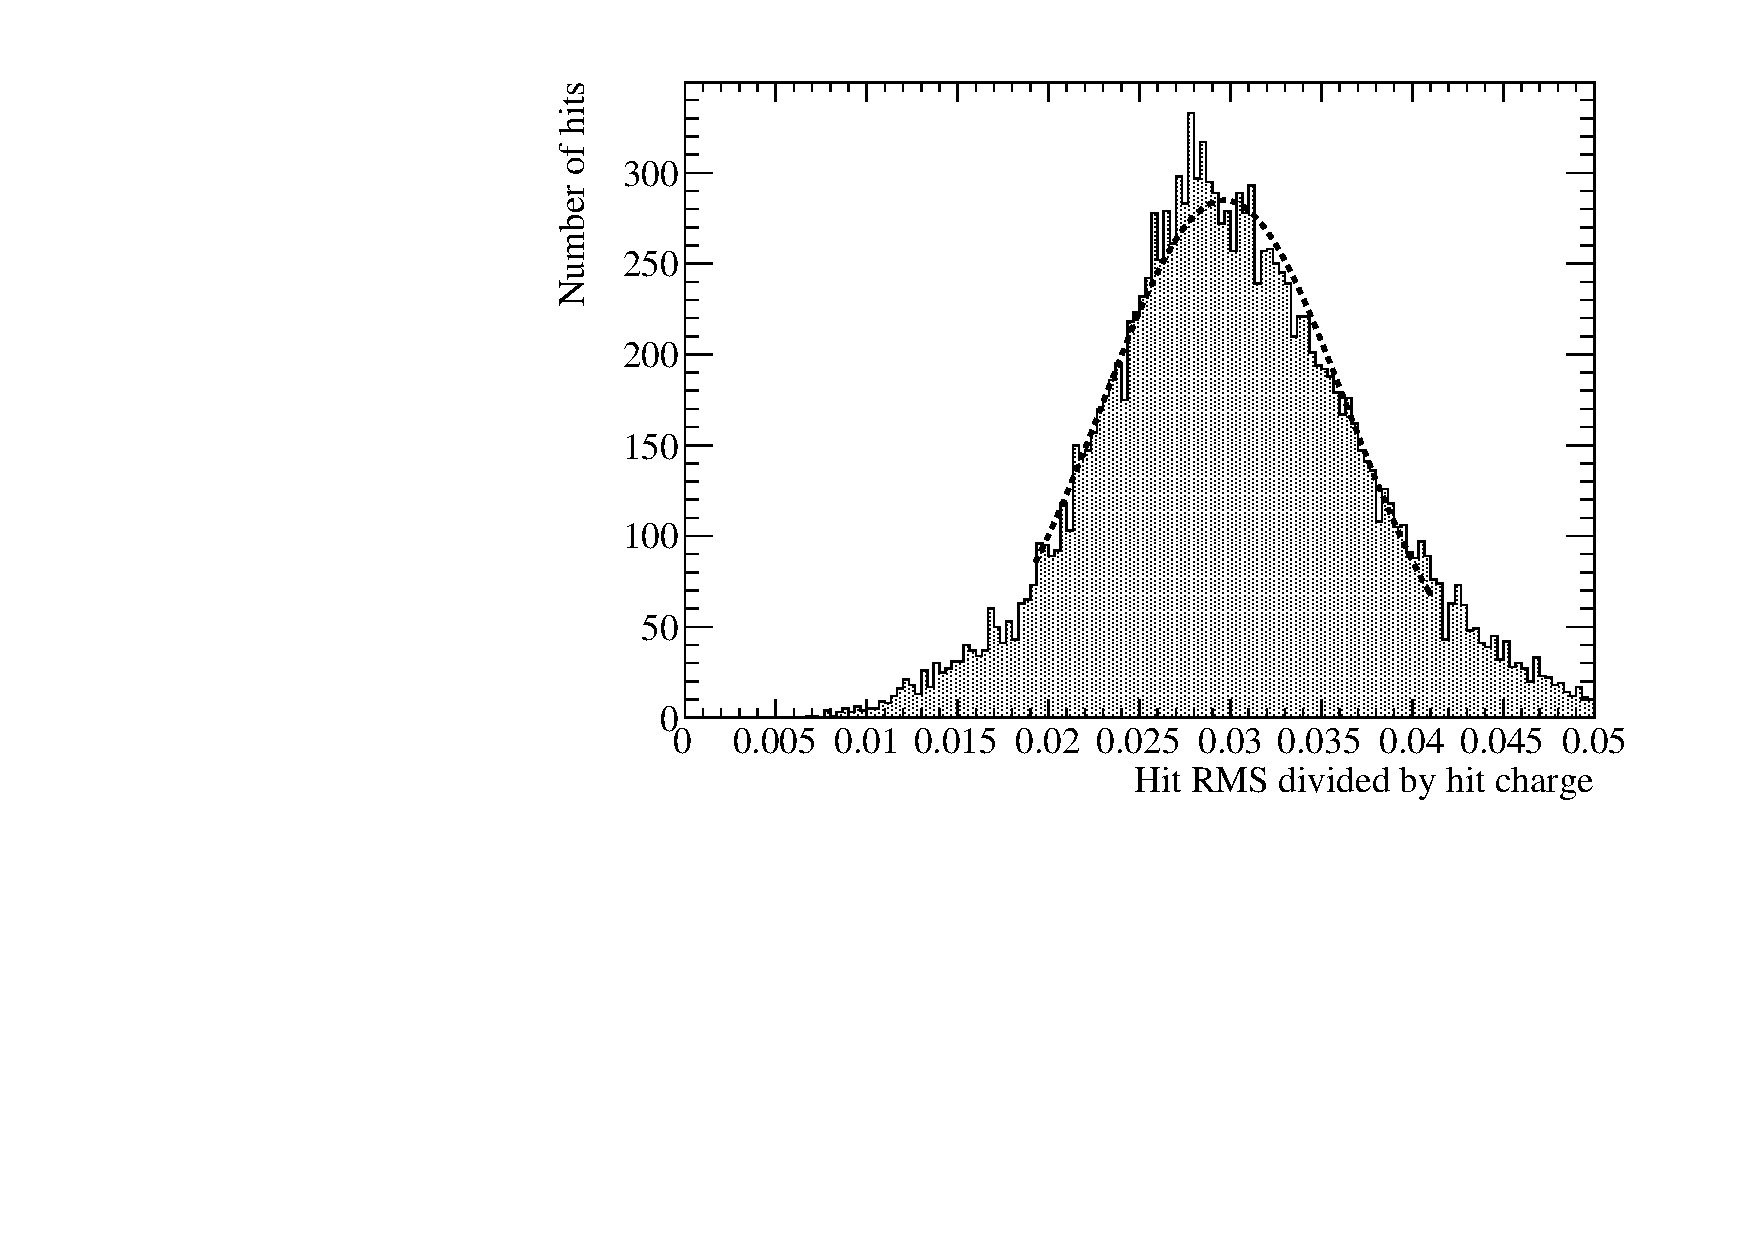
\includegraphics[width=\textwidth]{DataCan_3}
    \caption{The distribution of hit $RMS/Charge$ value for hits between $x =$ 140~cm and $x =$ 150~cm.}
  \end{subfigure}
  \caption[The distributions of the $RMS$ and $RMS/Charge$ values for tracks with a counter difference of 4 in the 35 ton data]
          {The distributions of hit $RMS$ (top), and hit $RMS/Charge$ (bottom), for points between 20 and 30~cm from the APAs (left), and points between 140 and 150~cm from the APAs (right), for tracks associated with coincidences that have a counter differences of 4. The most probable values of hit $RMS$ and hit $RMS/Charge$ are determined by fitting Gaussian functions around the peaks of the distributions. These fits are shown as dashed lines.}
          \label{fig:DiffDataHitFit}
\end{figure}

From Figure~\ref{fig:DiffDataHitFit} it is clear the the width of the hit $RMS$ distribution increases for hits which are further from the APAs. However, the width of the hit $RMS/Charge$ is seen to decrease, though this is due to a sharp cut-off at a hit $RMS/Charge$ equal to roughly 0.038~ticks$\cdot$ADC$^{-1}$. The reason for this cut off was shown in Figure~\ref{fig:TingjunLifetime}. It can also be seen that the most probable values of both the hit $RMS$ and hit $RMS/Charge$ increases with drift distance. \\

This drift distance effect can be observed by plotting the most probable values of hit $RMS$ and hit $RMS/Charge$, as drift distance increases, for fixed counter differences. This drift distance dependence on hit $RMS$ is shown in Figure~\ref{fig:CDiff4DataFit}, for tracks that are associated with a coincidence which had a counter difference of 4. A drift distance dependence can clearly be seen in the data, as the most probable hit $RMS$ is seen to increase for hits which originate further from the APAs. \\

\begin{figure}
  \centering
  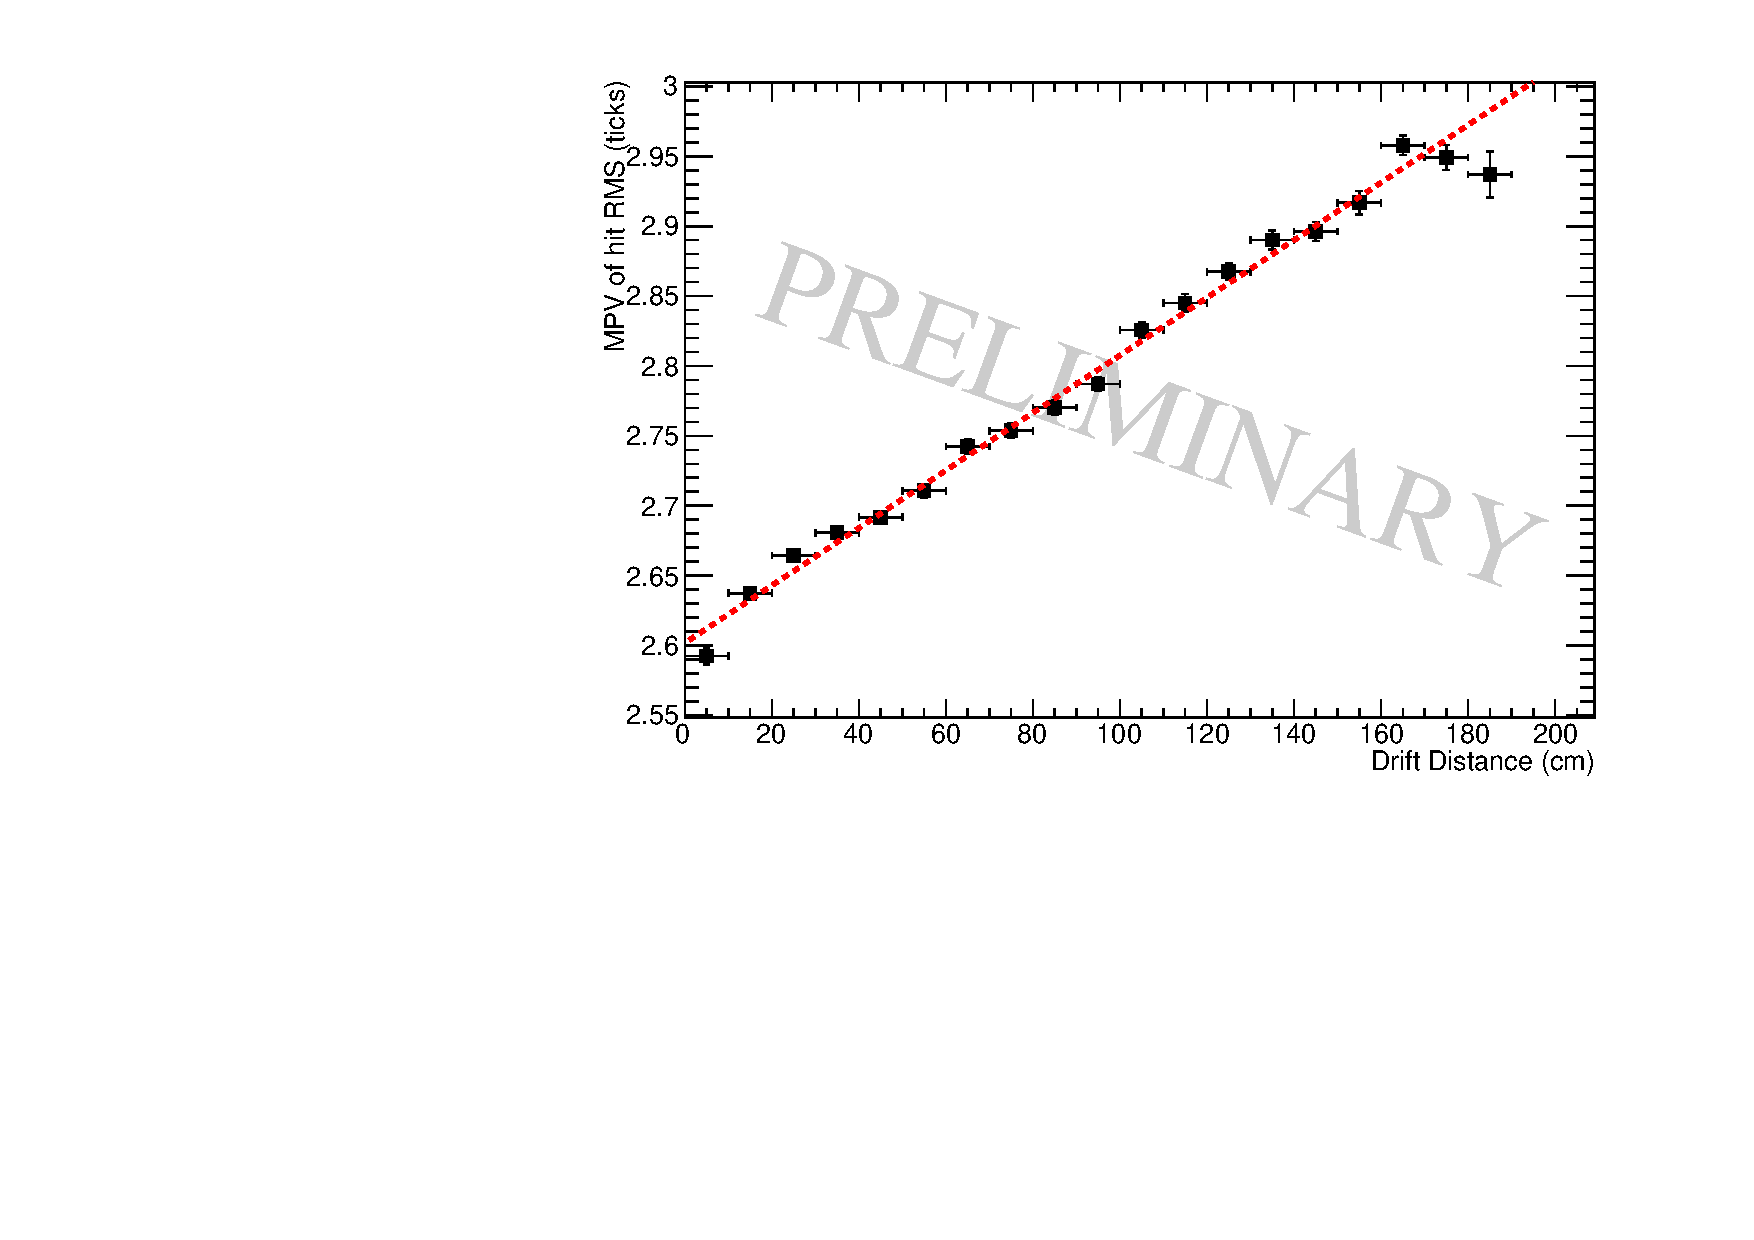
\includegraphics[width=0.6\textwidth]{CounterDiff4_Data}
  \caption[The drift distance dependence of diffusion in the 35 ton dataset for coincidences with a counter difference of 4]
          {The most probable values of hit $RMS$ as a function of drift distance, for the hits within a track, associated with a coincidence that had a counter difference of 4.}
  \label{fig:CDiff4DataFit}
\end{figure}

The angular dependence can then be shown by observing how the most probable fit values at a drift distance of 0~cm changes for increasing angles, this is shown in Figure~\ref{fig:DiffData_AngFit}. It is clear that there is an angular dependence on the hit width, as the most probable hit widths next to the APAs is seen to rise for tracks associated with coincidences with large counter differences. This angular dependence, along with the drift distance dependence, show that when considering a large sample, diffusion can be separated into distance and angular dependencies. However, whether this can be observed for individual tracks has not yet been considered. \\

\begin{figure}
  \centering
  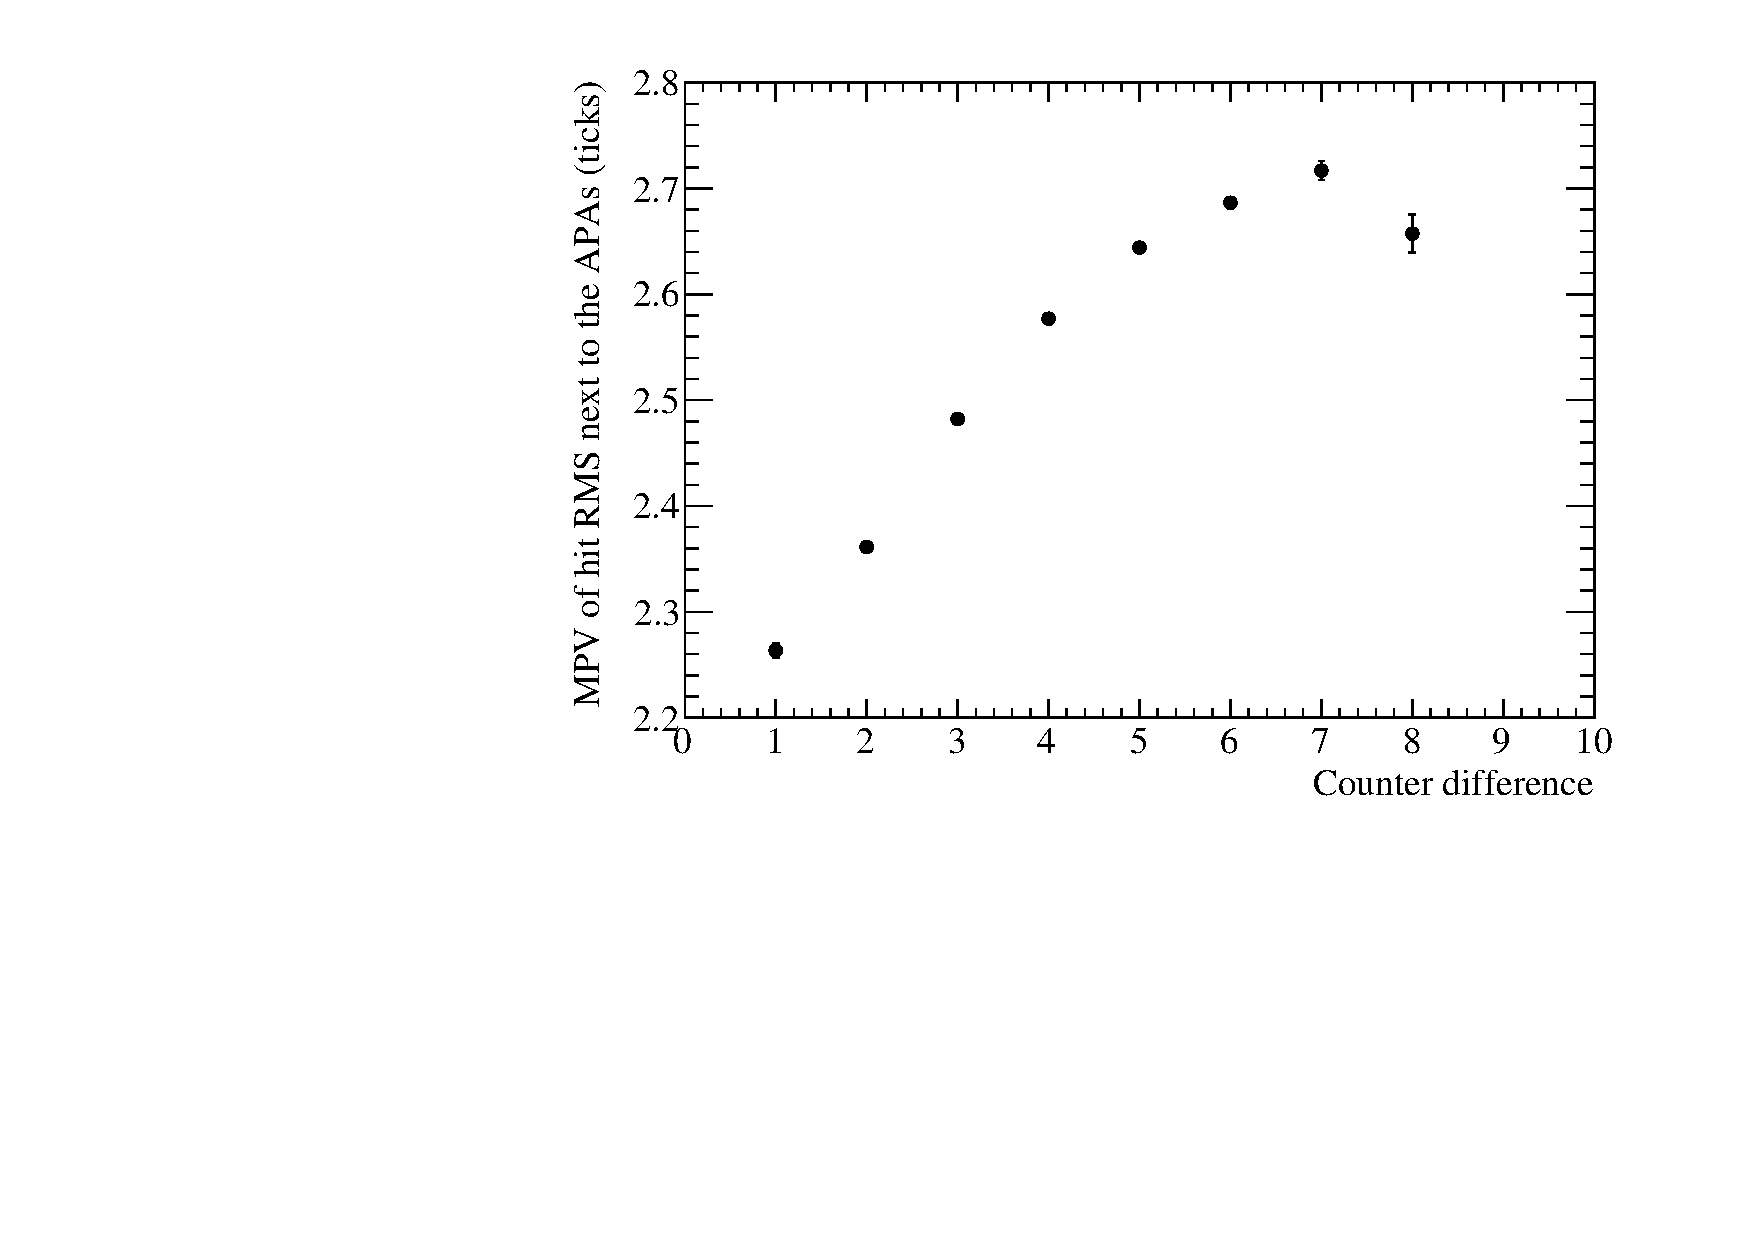
\includegraphics[width=0.6\textwidth]{InterceptCanvasData}
  \caption[The angular dependence of diffusion in the 35 ton dataset for hits within 10~cm of the APAs]
          {The most probable values of hit $RMS$ within 10~cm of the APAs, as a function of the counter difference of the coincidence, that the track, to which the hits belong, was associated with.}
  \label{fig:DiffData_AngFit}
\end{figure}

To consider single tracks, the best line fits for the counter differences for a large sample of tracks, such as in Figure~\ref{fig:CDiff4DataFit}, are required. These best line fits can then be used to predict the position you would expect a hit to originate from, given values for the hit $RMS$ and hit $RMS/Charge$, and the angle of the track to which it belongs. The predicted positions can then be compared to the known position from the counter coincidence to determine the accuracy of the prediction. \\

The distributions shown in Figure~\ref{fig:DiffDataHitFit} are asymmetric due to some hits having large values of hit $RMS$ or hit $Charge$. Asymmetry is also introduced by the threshold for hits. This comes about as a result of the elevated hit threshold, required to minimise the number of reconstructed noise hits, as shown in Figure~\ref{fig:TingjunLifetime}. Whilst nothing can be done retrospectively concerning the omission of the lowest charge hits, the highest charge hits, which cause the tails at low hit $RMS/Charge$, can be removed. This can be done by not using hits which are in the tails of the hit $Charge$ distribution. The tails of the distributions are removed by considering a plot of normalised hit charge, whereby the most probable hit charge has a value of 1. A conservative cut on normalised hit charges of 0.25 is made, so that it can be guaranteed that the tails are removed. This is shown in Figure~\ref{fig:DiffData_ChargeCut}. Any hits with charges less than $\sim$65~ADC, and any hits with charges more than $\sim$170~ADC are not used. This will have the effect of removing some of the low charge hits which were reconstructed, but the main effect will be the removal of the significant number of high charge hits, which introduce the tail at low hit $RMS/Charge$ (Figure~\ref{fig:DiffDataHitFit}). The difference in the predicted and reconstructed hit times should then be centred around the interaction time, and be distributed much more uniformly. This will mean that the interaction time can be determined much more accurately. \\

\begin{figure}
  \centering
  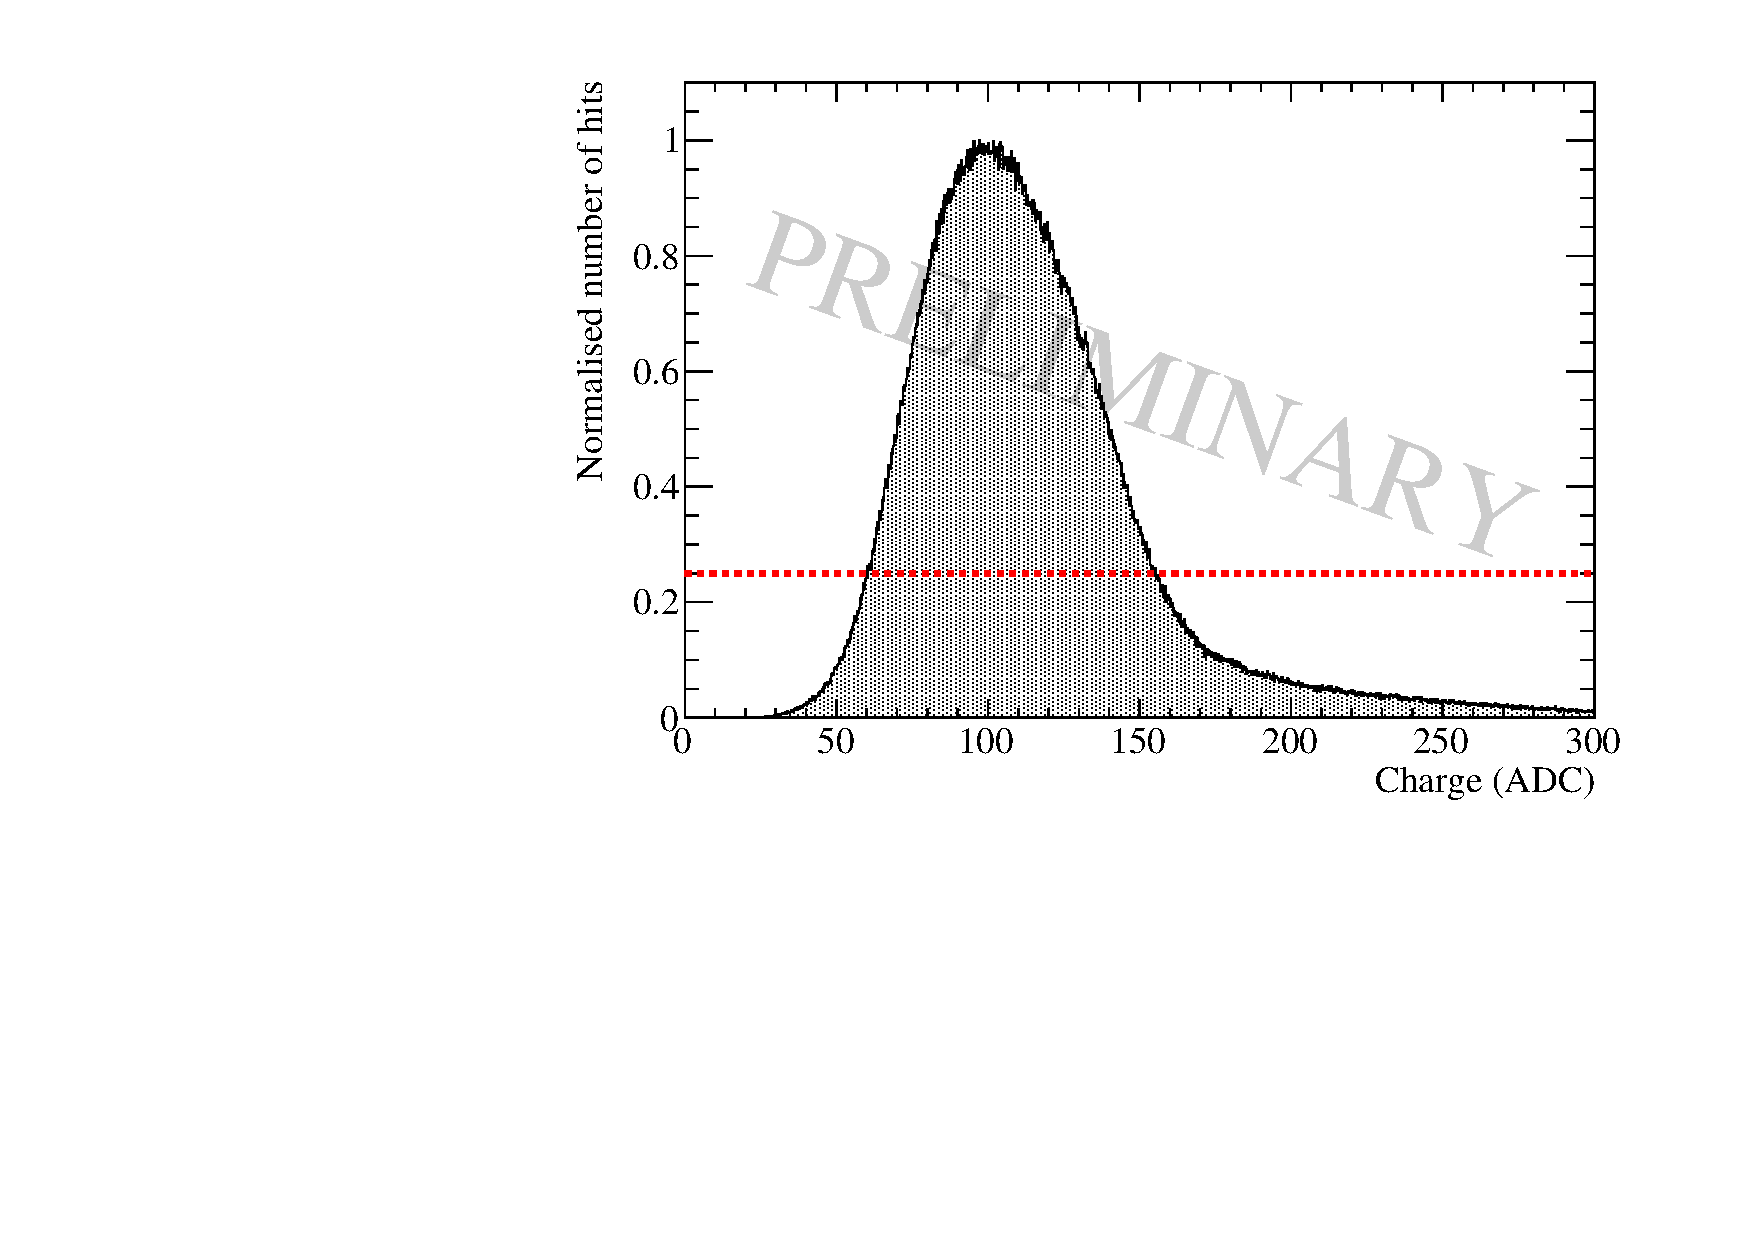
\includegraphics[width=0.6\textwidth]{ChargeCutData}
  \caption[The distribution of normalised hit charge in the 35 ton dataset]
          {The distribution of normalised hit charge, shown in units of ADC, in the 35 ton dataset. The number of hits with the most probable hit charge has been normalised to a value of 1. A cut on the normalised number of hits being greater than 0.25 is shown, the aim of this cut is to remove the tails of the hit charge distribution.}
  \label{fig:DiffData_ChargeCut}
\end{figure}

An intrinsic assumption in this method is that the track has a large number of collection plane hits, which do not contain delta rays, and are on wires which would not be identified as noisy. The tracks being considered here will have crossed all $z$ values in the detector, meaning that a total of 336 collection hits could potentially be reconstructed. Given the reconstruction problems in the 35 ton detector, very few tracks will have hits on all of these collection wires. However, requiring at least 100 collection plane hits is not unreasonable, and would correspond to a reconstructed track length of at least 50~cm. The difference between the predicted and reconstructed hit time for each hit is shown in Figure~\ref{fig:DiffDataPredHit}, for both the hit $RMS$ and hit $RMS/Charge$ metrics. \\

\begin{figure}
  \centering
  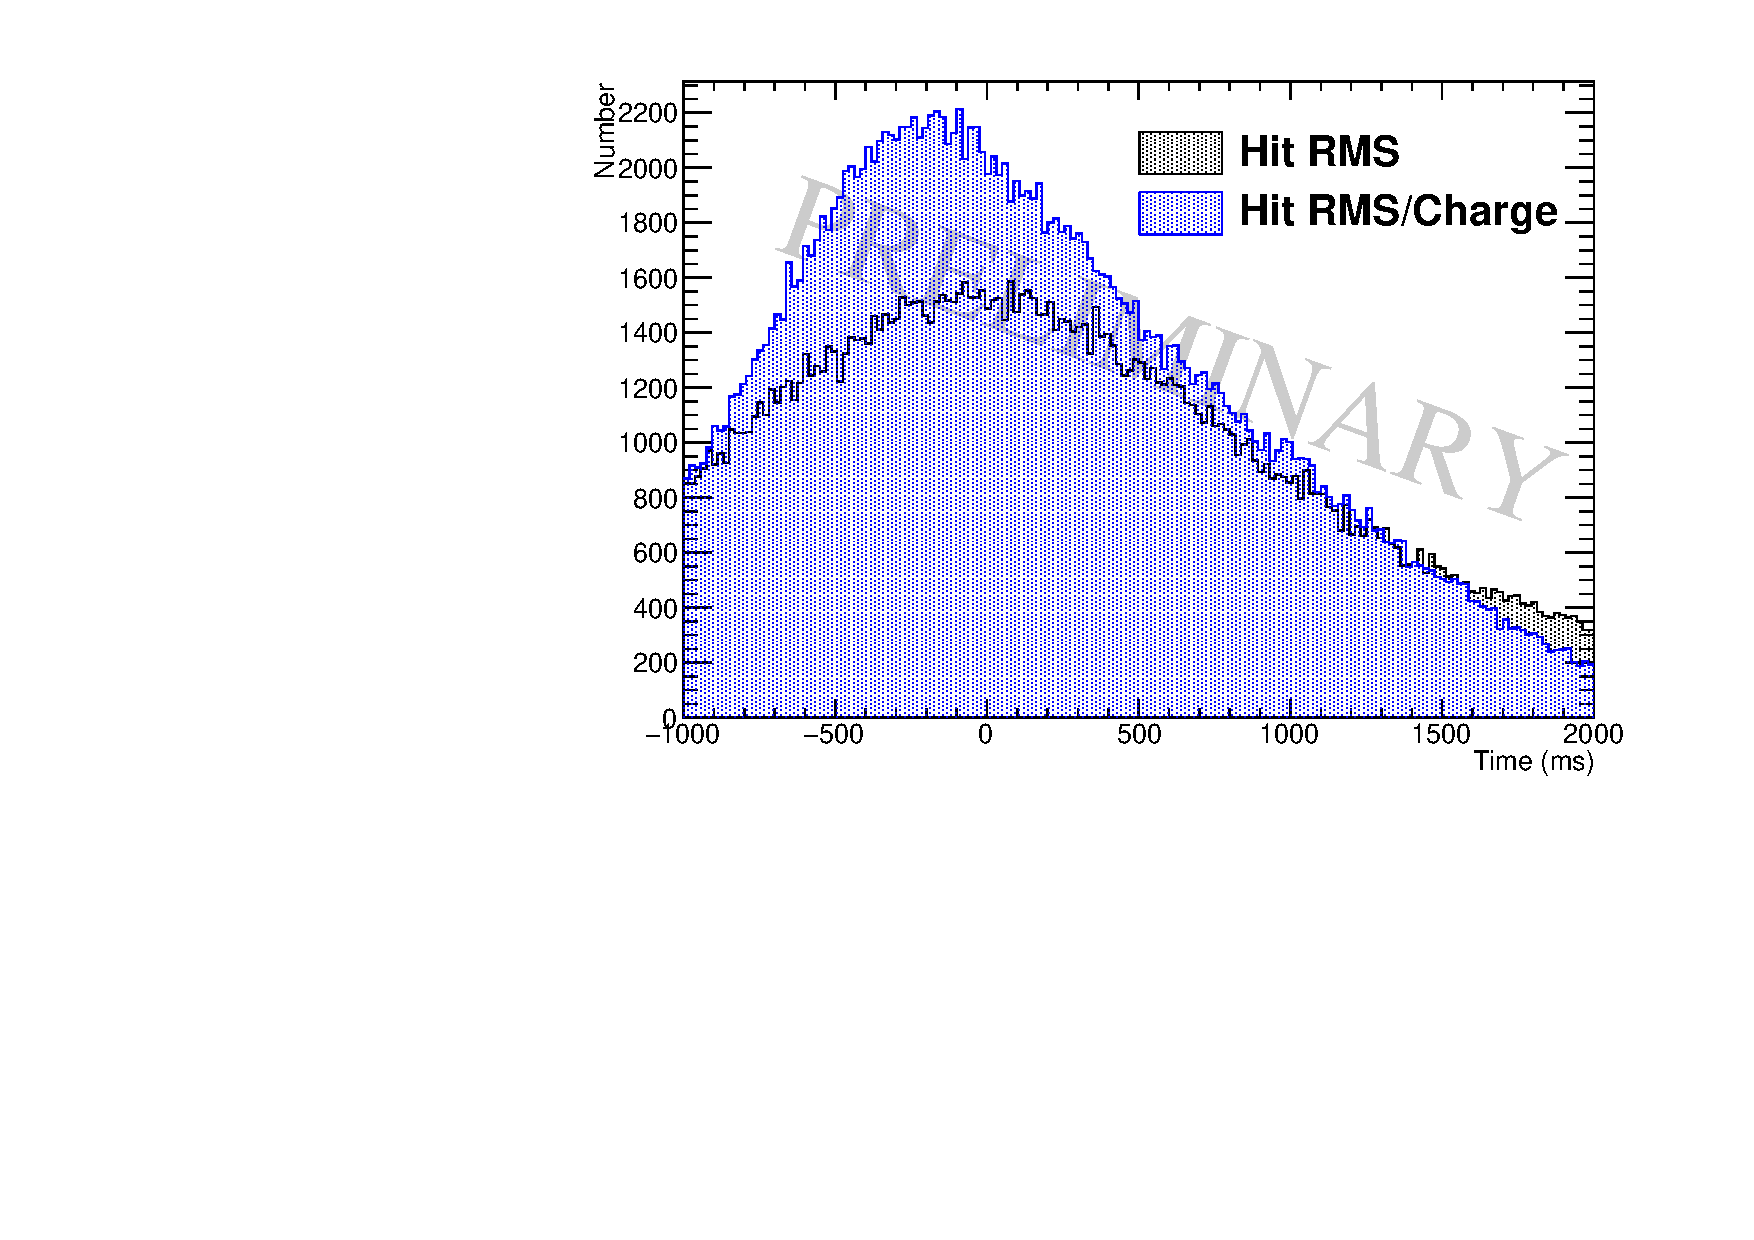
\includegraphics[width=0.6\textwidth]{DifferenceInteractionTime_Data}
  \caption[The difference between the predicted and reconstructed hit times in the 35 ton dataset]
          {The difference between the predicted and reconstructed hit times in the 35 ton dataset. The differences in time when the hit $RMS$ metric is used are shown in black, whilst the differences in time when the hit $RMS/Charge$ metric is used are shown in blue.}
  \label{fig:DiffDataPredHit}
\end{figure}

Figure~\ref{fig:DiffDataPredHit} shows that both distributions are centred around a time difference of 0~$\mu$s in the 35 ton dataset. This is encouraging as it shows that the method has potential. The width of the distribution for the $RMS/Charge$ metric is smaller, and the peak higher, so it is expected that this will provide the more robust metric. This is because these features show that the predicted hit times are likely to be close to the reconstructed hit times. The peaks are centred around a time difference of 0, as the hit times had previously been corrected using the measured interaction time from the counter coincidence. This was done so as to avoid the uncertainty which would arise from allowing the coincidences to remain at random times between ticks 5000 and 6000, in the 15000 tick event. For an explanation as to why this occurs, see the discussion concerning Figure~\ref{fig:DataStructure}. \\

It is interesting to observe the non-symmetric nature of the hit $RMS/Charge$ distribution which is seen in Figure~\ref{fig:DiffDataPredHit}. This is caused by there being a tendency for the prediction metric to overestimate the $x$ positions of the track. However, it is clearly evident that many of the predicted $x$ positions are highly accurate, as there is a definite peak around a difference in predicted and reconstructed hit times of 0~$\mu$s. When the difference in predicted and reconstructed hit times is plotted as a function of the central $x$ position of the counter coincidence, it is seen that this bias towards overestimating the interaction time comes from hits which are close to the APA frames. This suggests that the fit which was made in Figure~\ref{fig:DiffDataHitFit_RMSQ20} has produced an incorrect MPV. \\

When evaluating interaction times, the average difference in reconstructed and predicted hit times across every hit on the track must be considered. This average difference in reconstructed and predicted hit times, is calculated by taking the sum of the individual differences in reconstructed and predicted hit times for every collection plane hit in the track, and dividing this by the number of collection plane hits in the track. This is shown in Figures~\ref{fig:DiffDataAvDiff_RMS} and~\ref{fig:DiffDataAvDiff_RMS_Int}, where, as expected from Figure~\ref{fig:DiffDataPredHit}, the $RMS/Charge$ metric provides a better estimation of the interaction time. The reason for this is that by utilising the charge information due to losses from impurities, this metric gains an extra handle on the drift distance, and hence the reconstructed time of the hits. The losses due to impurities may be difficult to measure in very high-purity LAr environments, as the decrease in collected charge with increasing drift distances is small~\citep{LongBo}. The effect of increasing LAr purity is shown in Section~\ref{sec:DiffMCStudies}. Using the change in hit charge in the 35 ton may have a drawback though, because, as shown in Figure~\ref{fig:TingjunLifetime}, there is a threshold effect for hits with large drift times. However, as the same threshold effect is present in all 35 ton data samples, the limitation it introduces is mainly in the efficiency with which ``good'' collection plane hits will be reconstructed, and so this information can be confidently used. \\

\begin{figure}
  \centering
  \begin{subfigure}{0.6\textwidth}
    \centering
    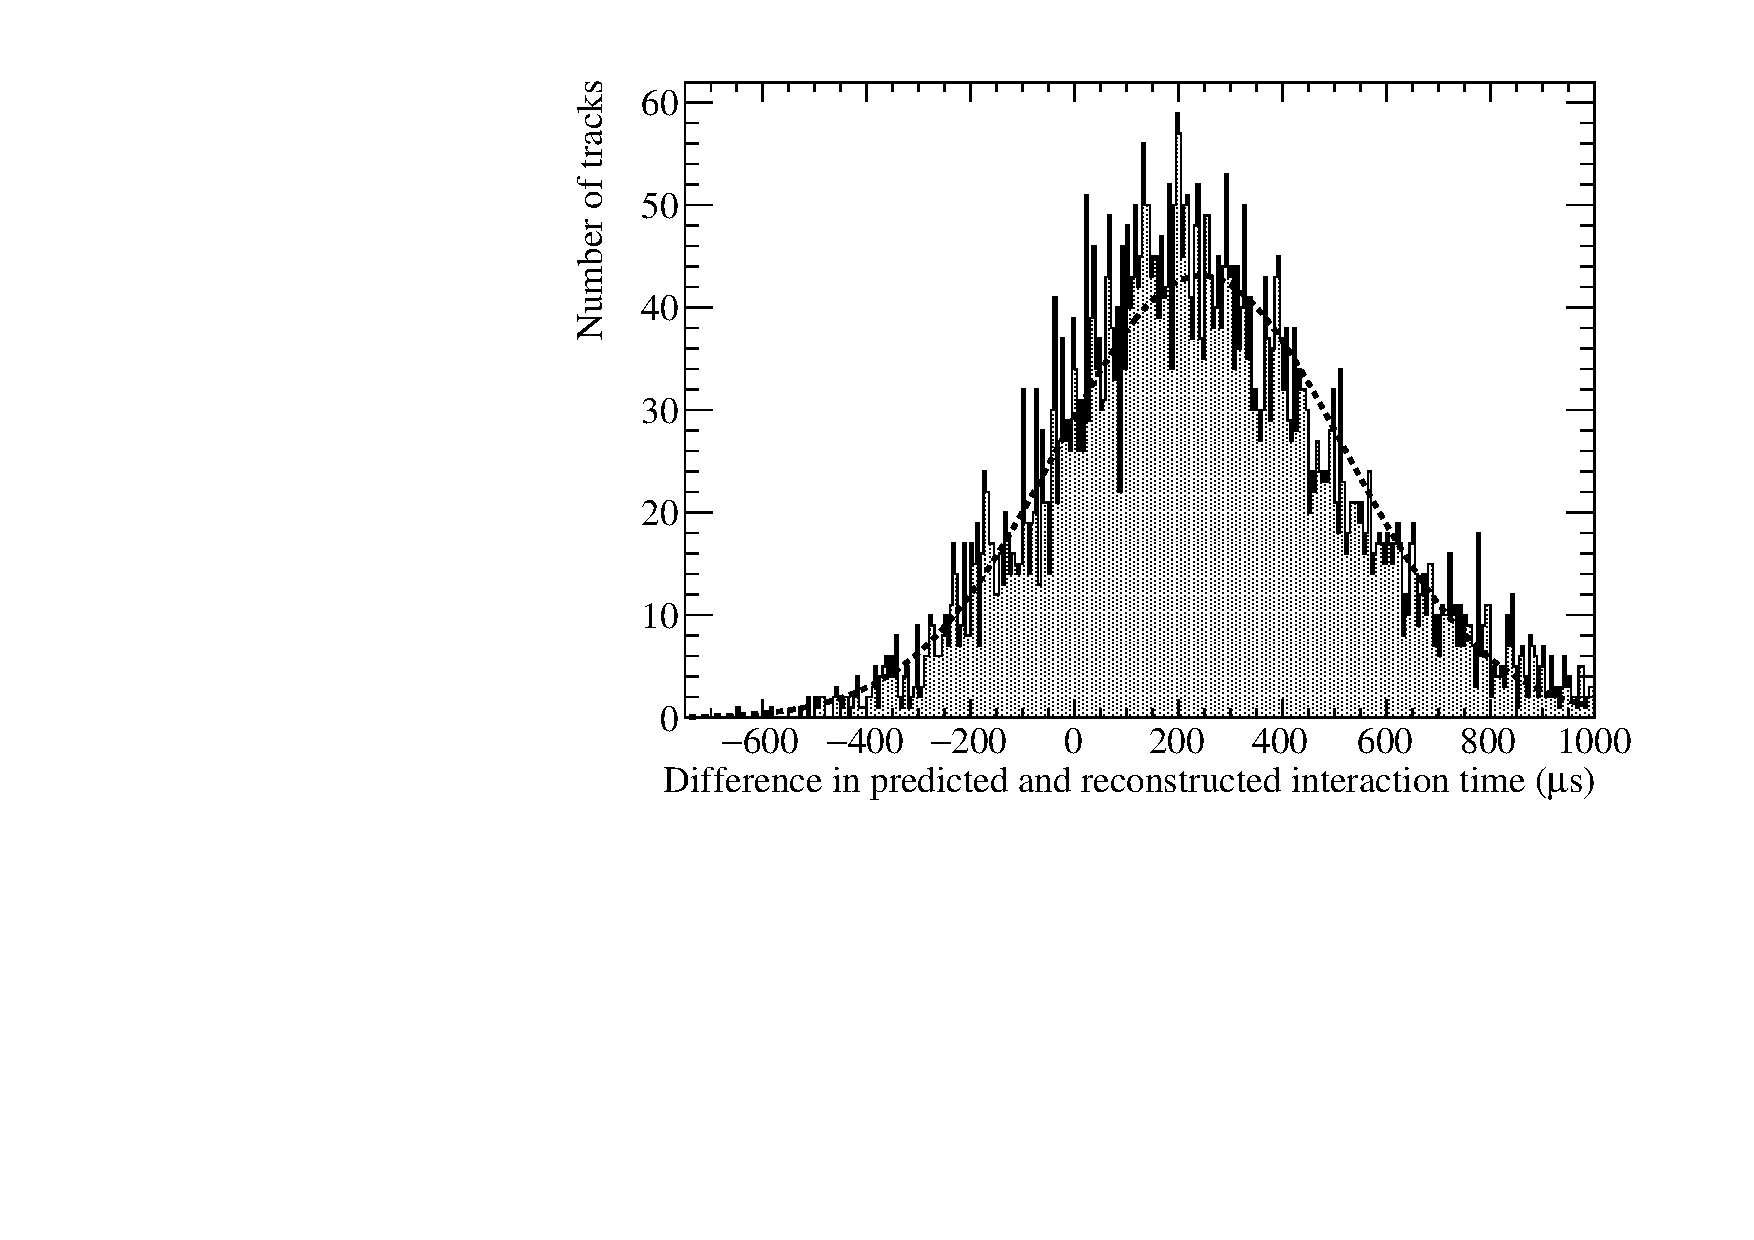
\includegraphics[width=\textwidth]{Data_AvTimeDiff_RMS}
    \caption{The average difference in interaction times using the hit $RMS$ metric.}
    \label{fig:DiffDataAvDiff_RMS_T}
  \end{subfigure}

  \begin{subfigure}{0.6\textwidth}
    \centering
    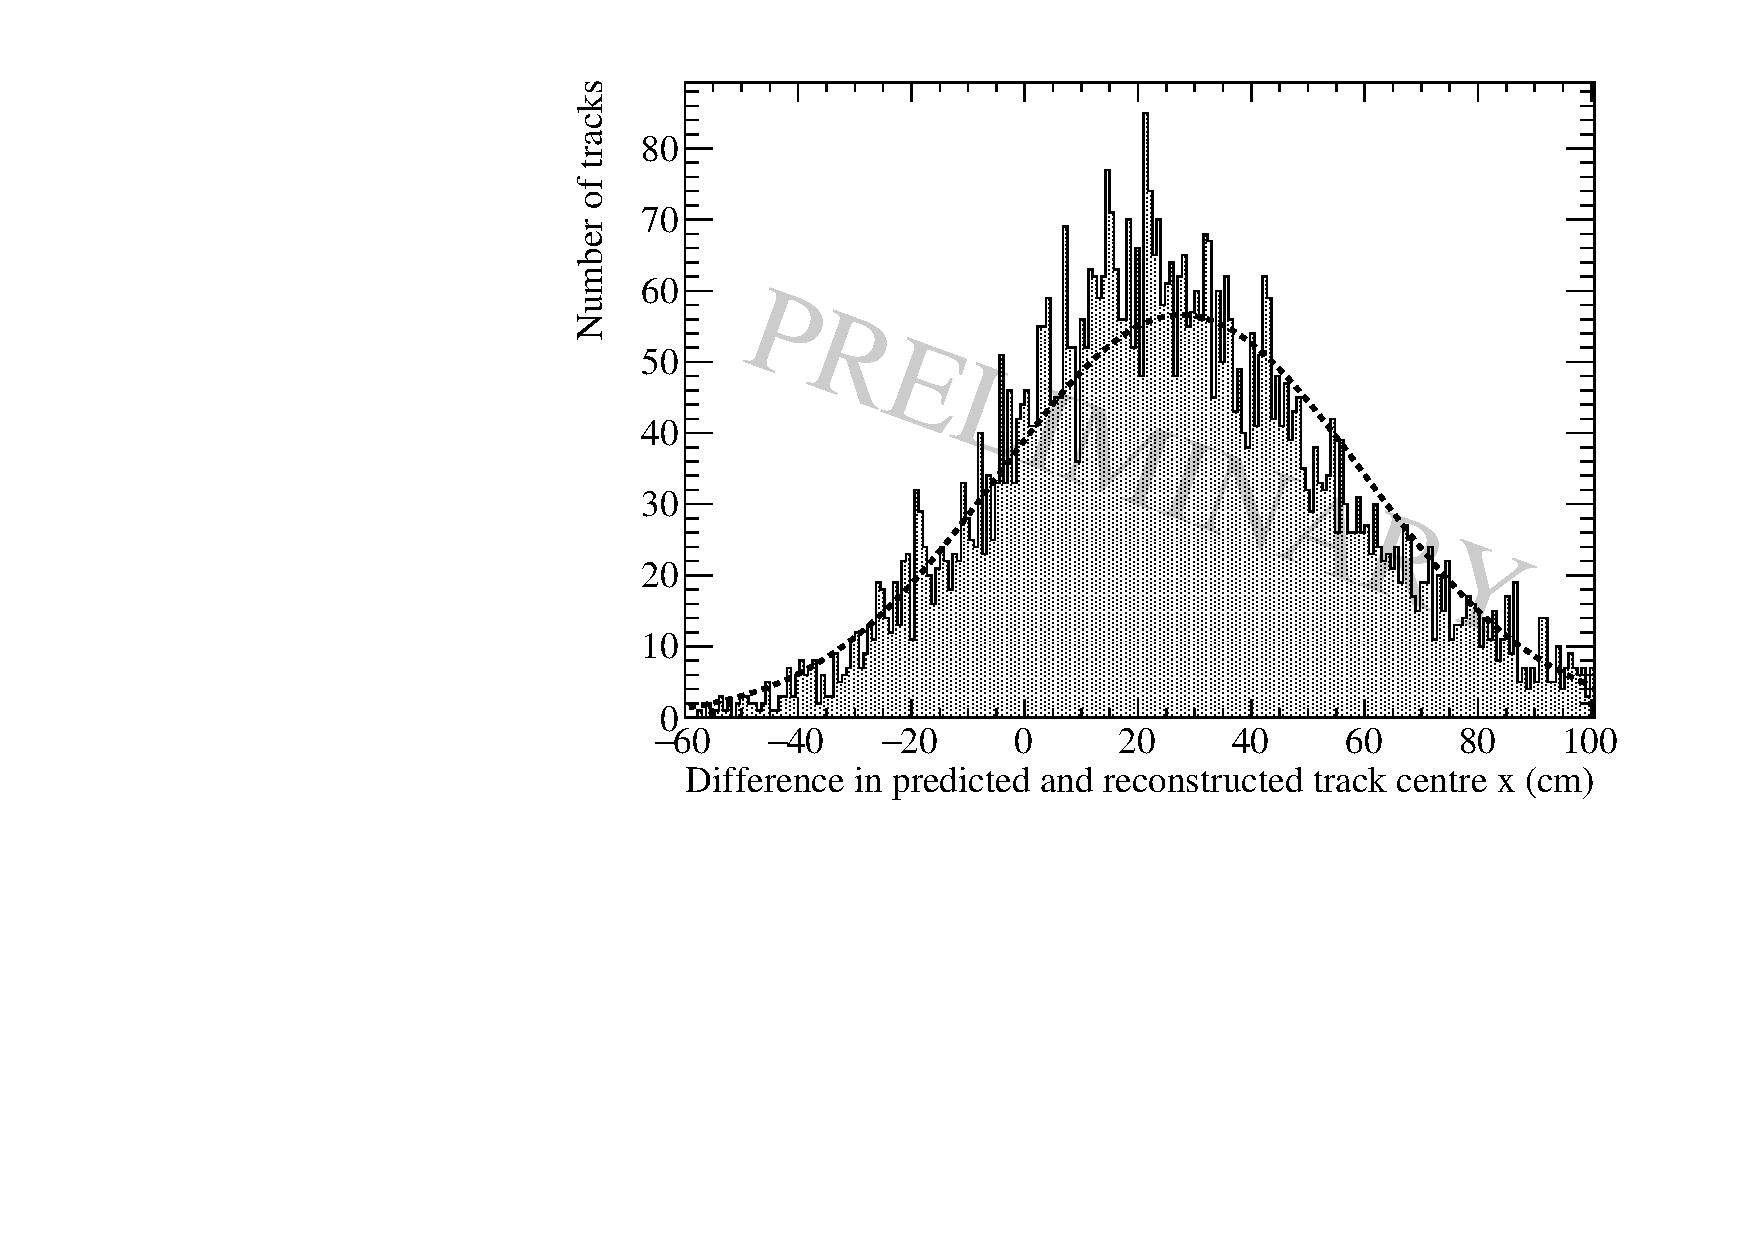
\includegraphics[width=\textwidth]{Data_AvXPosDiff_RMS}
    \caption{The average difference in the central $x$ position of a track using the hit $RMS$ metric.}
    \label{fig:DiffDataAvDiff_RMS_X}
  \end{subfigure}
  \caption[The accuracy of the hit $RMS$ method in the 35 ton dataset]
          {The accuracy of the hit $RMS$ method in the 35 ton dataset. Top: the accuracy to which interaction times can be determined in $\mu$s. Bottom: the accuracy to which the central $x$ position of a track can be determined. The average time difference ($x$ position) is calculated by taking the sum of individual hit differences for every hit in the track, and dividing this by the number of hits in the track. Gaussian functions are fitted to the distributions so that any offset in the predicted times or positions can be discerned. }
  \label{fig:DiffDataAvDiff_RMS}
\end{figure}

Figure~\ref{fig:DiffDataAvDiff_RMS} shows that using the effects of diffusion, and the hit $RMS$, the interaction time and central $x$ position of a track, can be reliably predicted in the 35 ton dataset. The accuracy in determining the interaction time is found to be 240~$\mu$s, where the distribution has a FWHM of 281~$\mu$s. When this is converted into the difference in central $x$ position of the track, the accuracy is found to be 27.7~cm, with a FWHM of 32.1~cm. \\

\begin{figure}
  \centering
  \begin{subfigure}{0.6\textwidth}
    \centering
    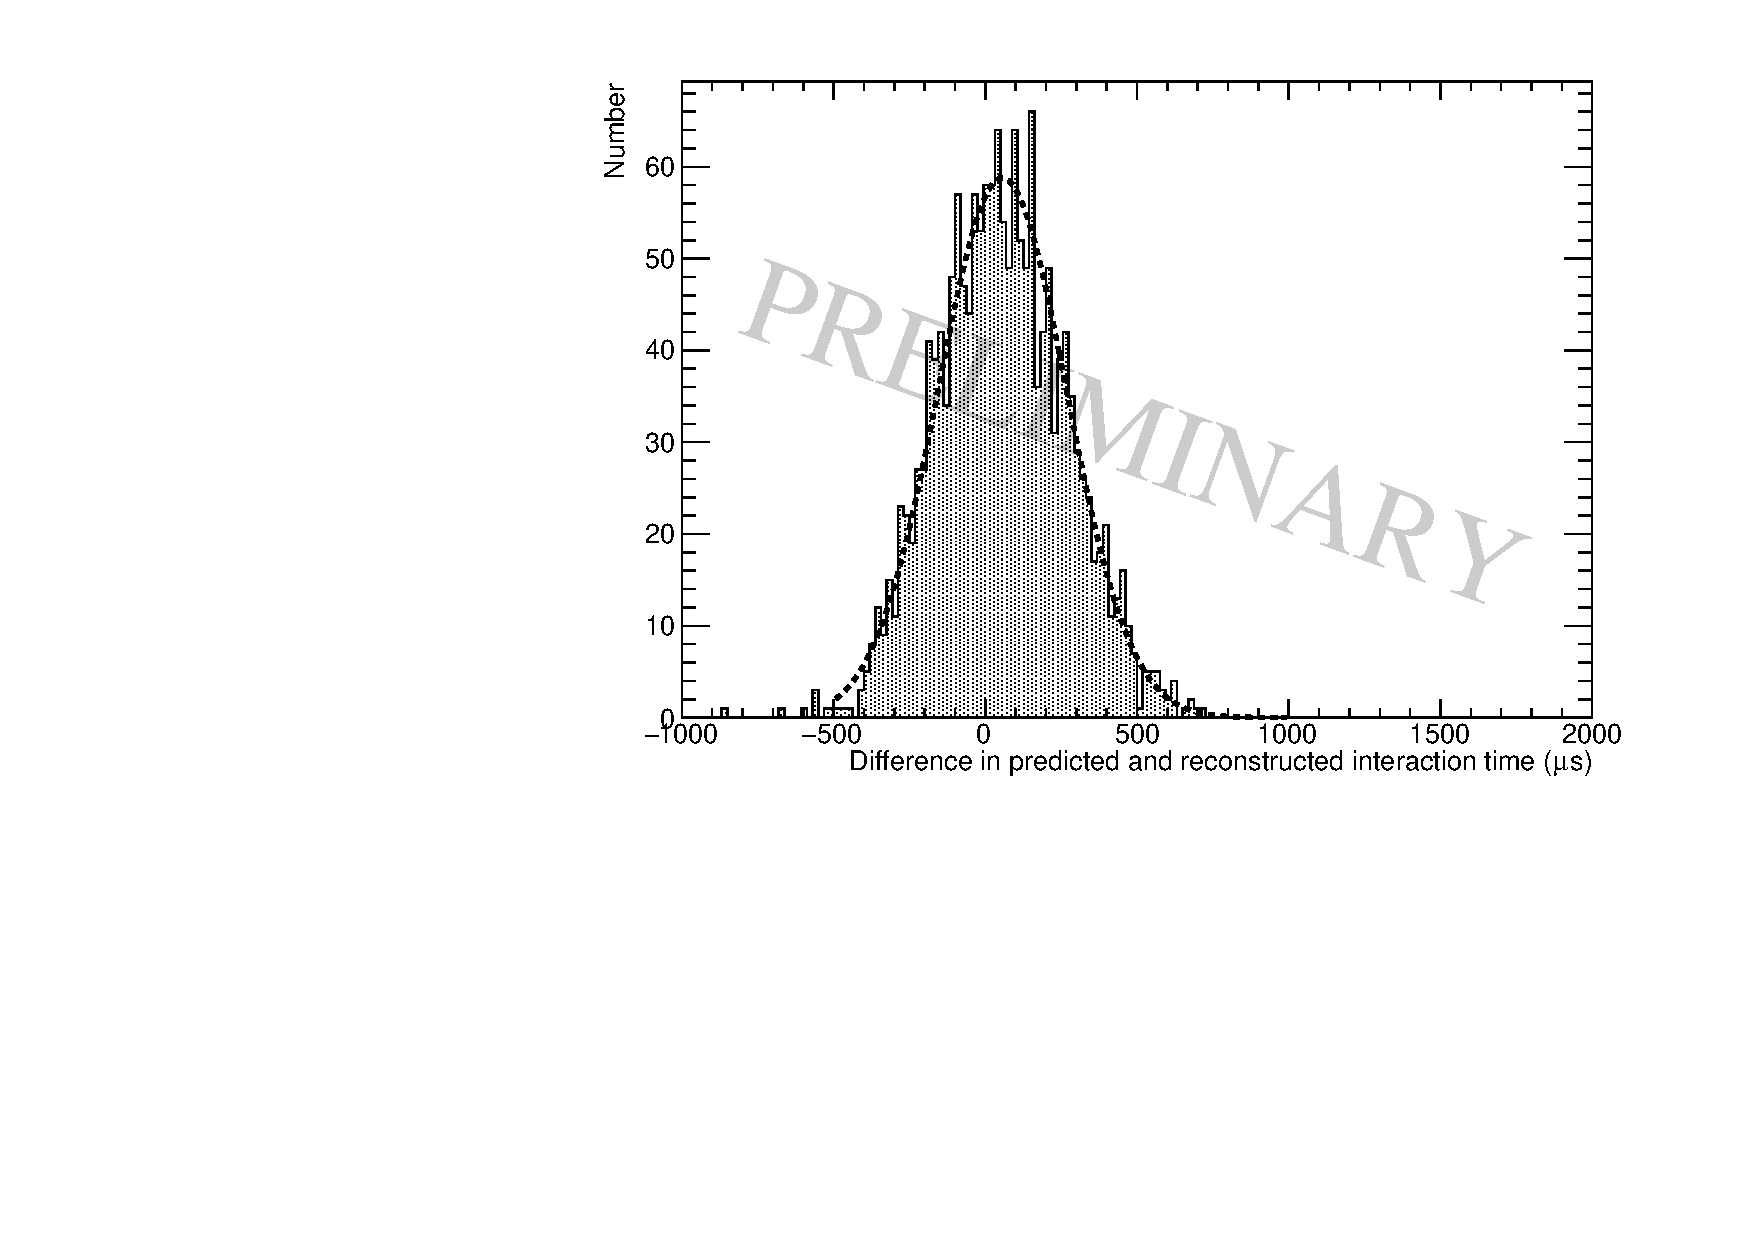
\includegraphics[width=\textwidth]{Data_AvTimeDiff_RMS_Int}
    \caption{The average difference in interaction times using the hit $RMS/Charge$ metric.}
    \label{fig:DiffDataAvDiff_RMS_Int_T}
  \end{subfigure}

  \begin{subfigure}{0.6\textwidth}
    \centering
    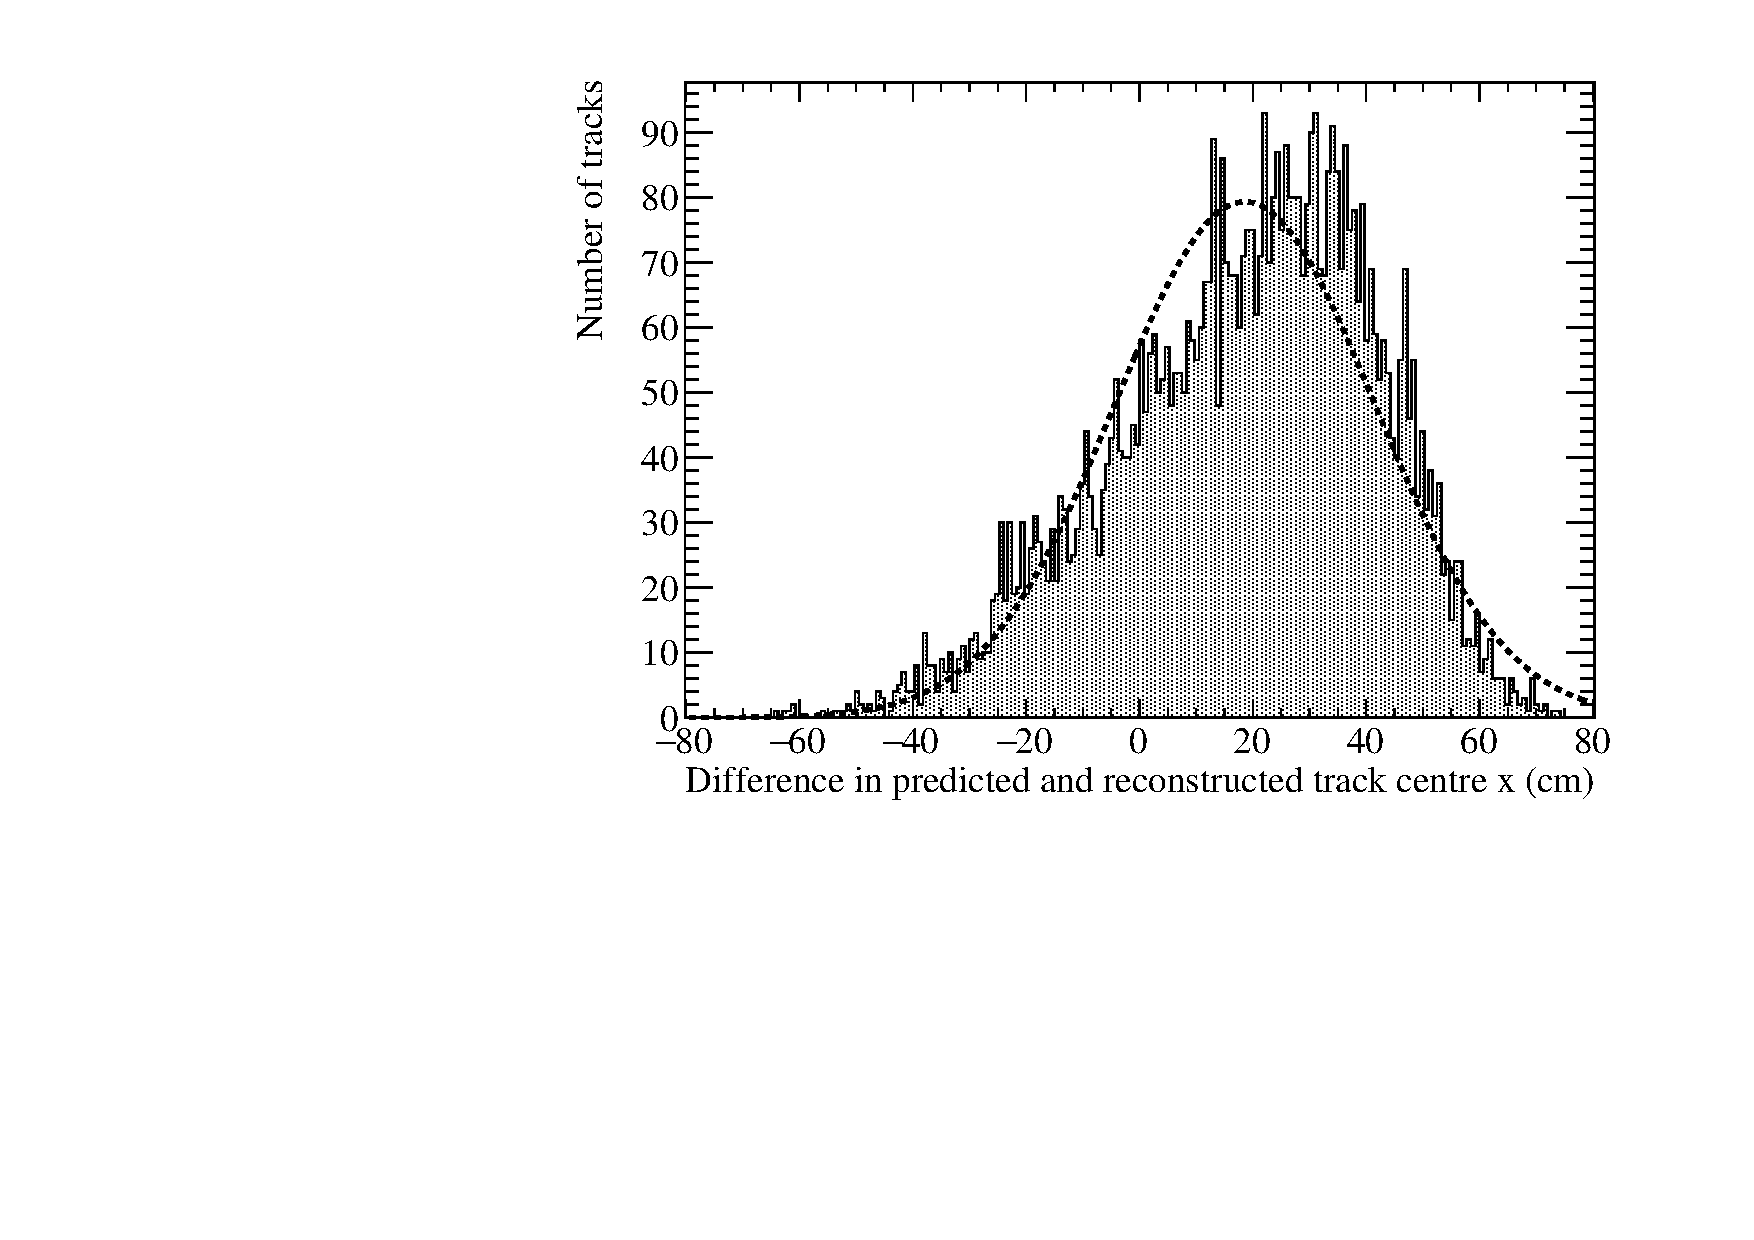
\includegraphics[width=\textwidth]{Data_AvXPosDiff_RMS_Int}
    \caption{The average difference in the central $x$ position of a track using the hit $RMS/Charge$ metric.}
    \label{fig:DiffDataAvDiff_RMS_Int_X}
  \end{subfigure}
  \caption[The accuracy of the hit $RMS/Charge$ method in the 35 ton dataset]
          {The accuracy of the hit $RMS/Charge$ method in the 35 ton dataset. Top: the accuracy to which interaction times can be determined in $\mu$s. Bottom: the accuracy to which the central $x$ position of a track can be determined. The average time difference ($x$ position) is calculated by taking the sum of individual hit differences for every hit in the track, and dividing this by the number of hits in the track. Gaussian functions are fitted to the distributions so that any offset in the predicted times or positions can be discerned.}
  \label{fig:DiffDataAvDiff_RMS_Int}
\end{figure}

Figure~\ref{fig:DiffDataAvDiff_RMS_Int} shows that using the effects of diffusion, and the hit $RMS/Charge$, the interaction time and central $x$ position of a track, can be reliably predicted in the 35 ton dataset. The accuracy in determining the interaction time is found to be 171~$\mu$s, where the distribution has a FWHM of 210~$\mu$s. When this is converted into the difference in central $x$ position of the track, the accuracy is found to be 18.5~cm, with a FWHM of 23.0~cm. \\

The resolutions found are quite impressive, as given that the total drift time for electrons through the whole 35 ton detector volume of 223~cm is roughly 5200~ticks, it means that tracks can be cleanly distinguished throughout the detector volume. Though the resolution of the interaction time determination is impressive, it is concerning that there appears to be a systematic offset which has been introduced. This is seen by the distributions not being centred around a difference in predicted and reconstructed times of 0~$\mu$s, as would be expected from the discussion concerning Figure~\ref{fig:DiffDataPredHit}. As discussed earlier, the issues with noise in the 35 ton dataset affect the accuracy with which tracking and calorimetry can be performed, and so it is reasonable to expect that the effectiveness of the interaction time determination was also affected. Therefore, it is prudent to repeat the study on a Monte Carlo sample, with the same detector conditions, but a much lower level of detector noise. This is presented in Section~\ref{sec:MCDataComp}. \\

%********************************** % Fifth.Second Section  *************************************
\subsection{Determining interaction times in a low-noise detector using Monte Carlo, and differences with data} \label{sec:MCDataComp}
When determining interaction times in Monte Carlo simulations, exactly the same criteria are applied to the hits. This is because $\delta$-rays would still change the measured hit width, and will be present in any sample. In a low noise detector it is expected that few wires would be removed due to being noisy, but for consistency there is no danger in applying this cut. Imposing a minimum number of collection plane hits is again important to ensure that the distribution of predicted hit times is centred on the interaction time. In addition to the same criteria being imposed on which wires are used, the same metrics are calculated. In all plots shown below the Monte Carlo dataset has been normalised to the size of the 35 ton dataset. This was done so that the area of the plots shown was the same, enabling easier comparison between the two datasets. \\

Figure~\ref{fig:DiffMCHitFit} shows both the hit $RMS$ and hit $RMS/Charge$ distributions, for hits from tracks that are associated with a coincidence that has a counter difference of 4, and are between 20~cm and 30~cm away from the APAs, or between 140~cm and 150~cm from the APAs. It can seen that there is a large difference in the distributions for hits which are relatively close to the APAs, at distances between 20~cm and 30~cm. The distributions are also much more tightly distributed in the Monte Carlo sample, showing that the variation between hits is much smaller. However, the difference between the Monte Carlo and 35 ton data samples are much smaller at large drift distances, showing that at large distances the distributions become much more varied. An important feature of the 35 ton data sample, which is not present in the Monte Carlo sample, is the sudden cut off in values of high hit $RMS/Charge$. This was briefly discussed in the consideration of Figure~\ref{fig:DiffDataHitFit}, but it is much clearer in Figure~\ref{fig:DiffMCHitFit_3}, where the rapid decrease in the number of hits with values of hit $RMS/Charge$ which are more than 0.038~ticks$\cdot$ADC$^{-1}$ seen in the 35 ton dataset, is not repeated in the Monte Carlo sample. This, along with Figure~\ref{fig:TingjunLifetime}, shows clear evidence that the hits with low values of hit $charge$ are not reconstructed in the 35 ton data sample. \\  

\begin{figure}
  \centering
  \begin{subfigure}{0.48\textwidth}
    \centering
    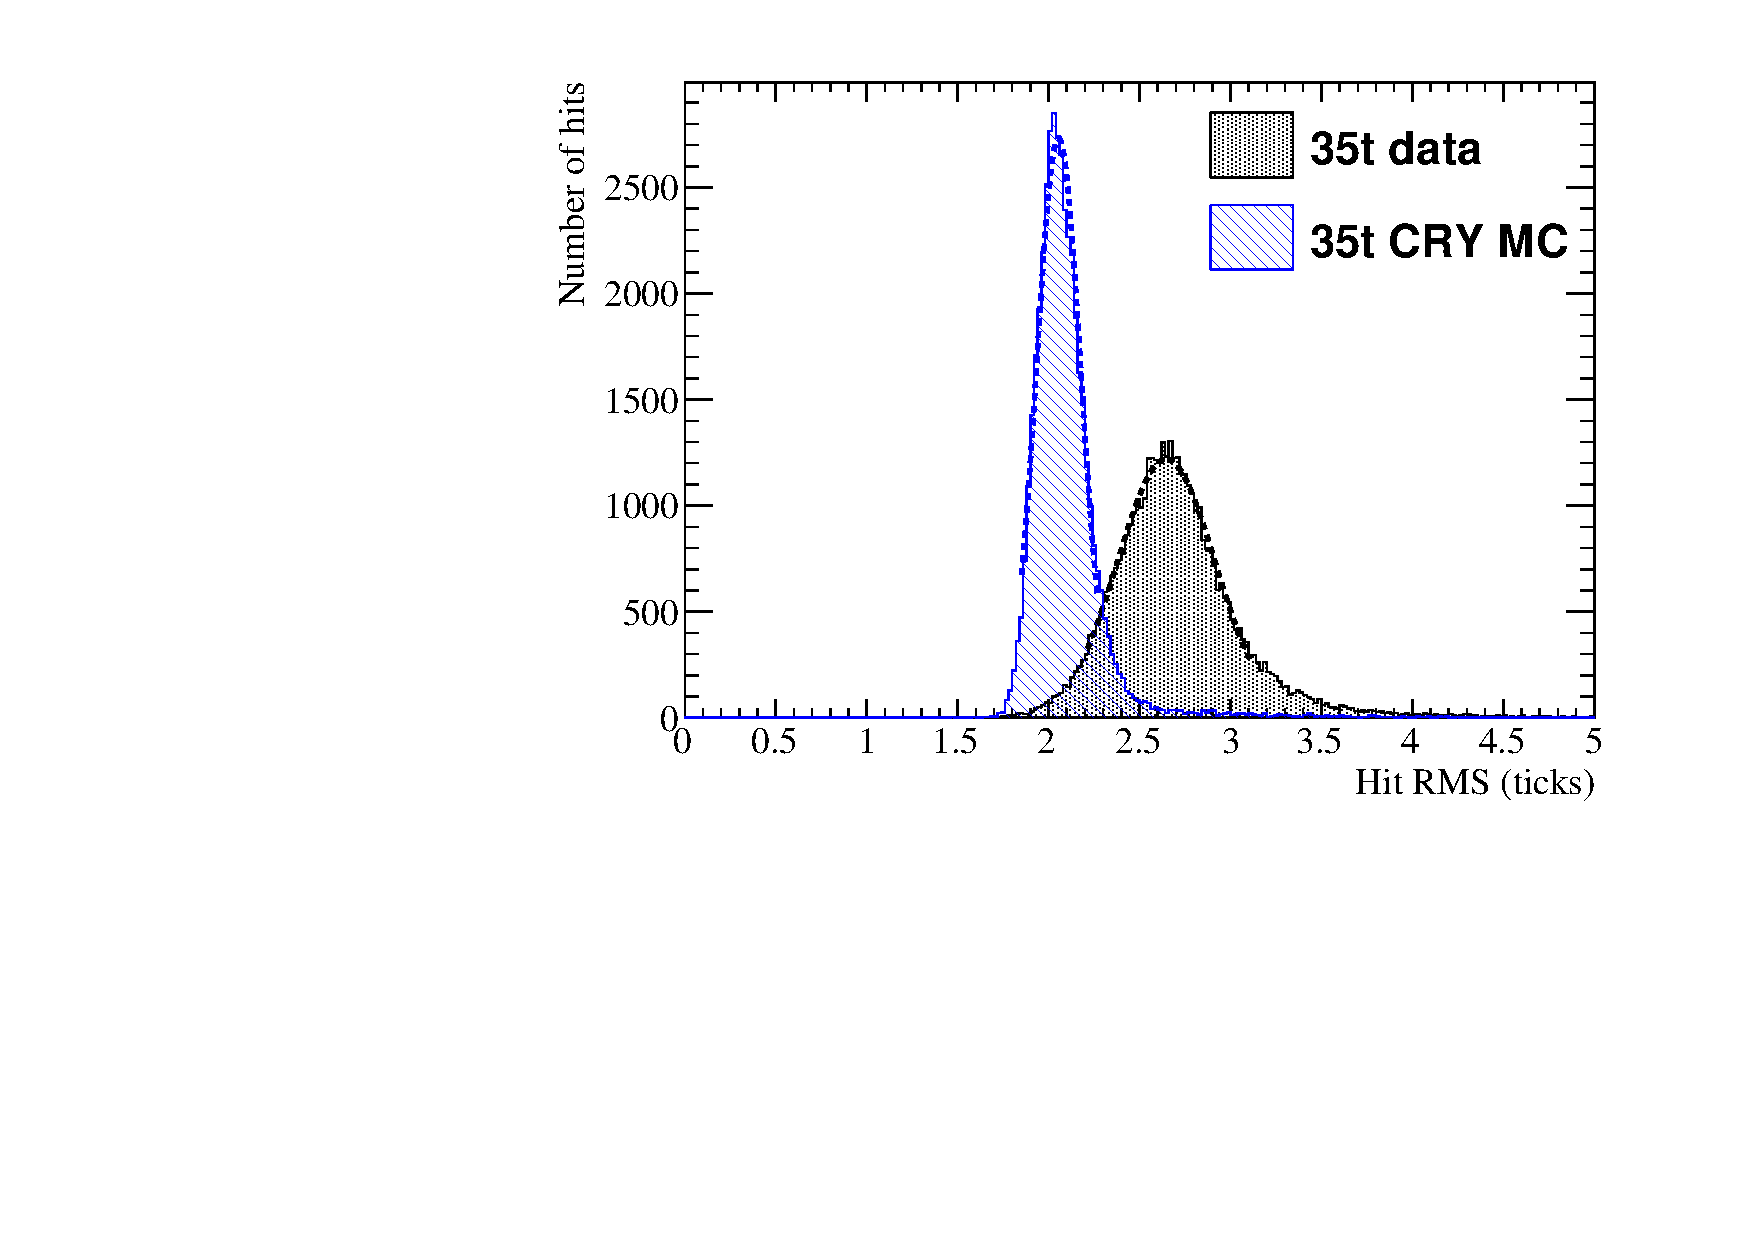
\includegraphics[width=\textwidth]{CombCan_0}
    \caption{The distribution of hit $RMS$ value for hits between $x =$ 20~cm and $x =$ 30~cm.}
  \end{subfigure}%
  \hspace{0.03\textwidth}%
  \begin{subfigure}{0.48\textwidth}
    \centering
    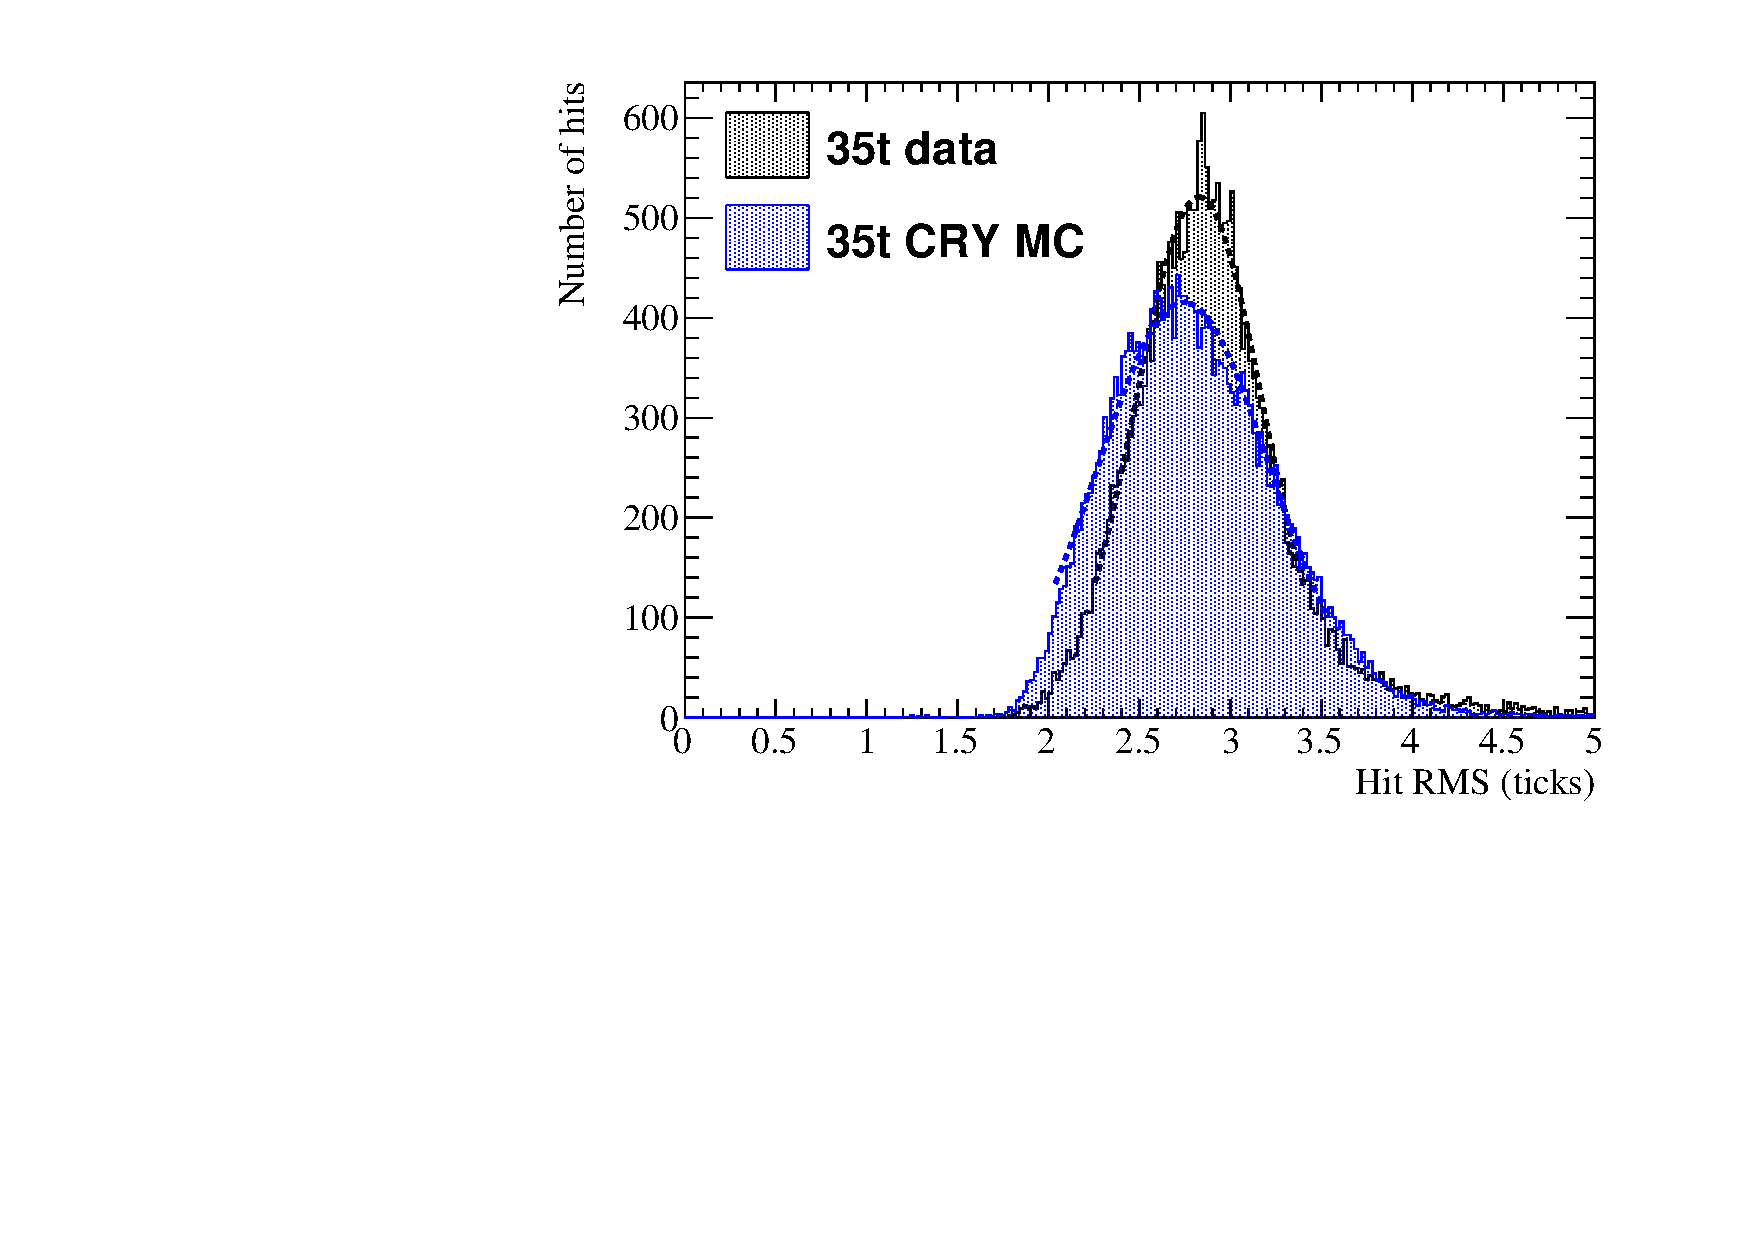
\includegraphics[width=\textwidth]{CombCan_1}
    \caption{The distribution of hit $RMS$ value for hits between $x =$ 140~cm and $x =$ 150~cm.}
  \end{subfigure}
  \begin{subfigure}{0.48\textwidth}
    \centering
    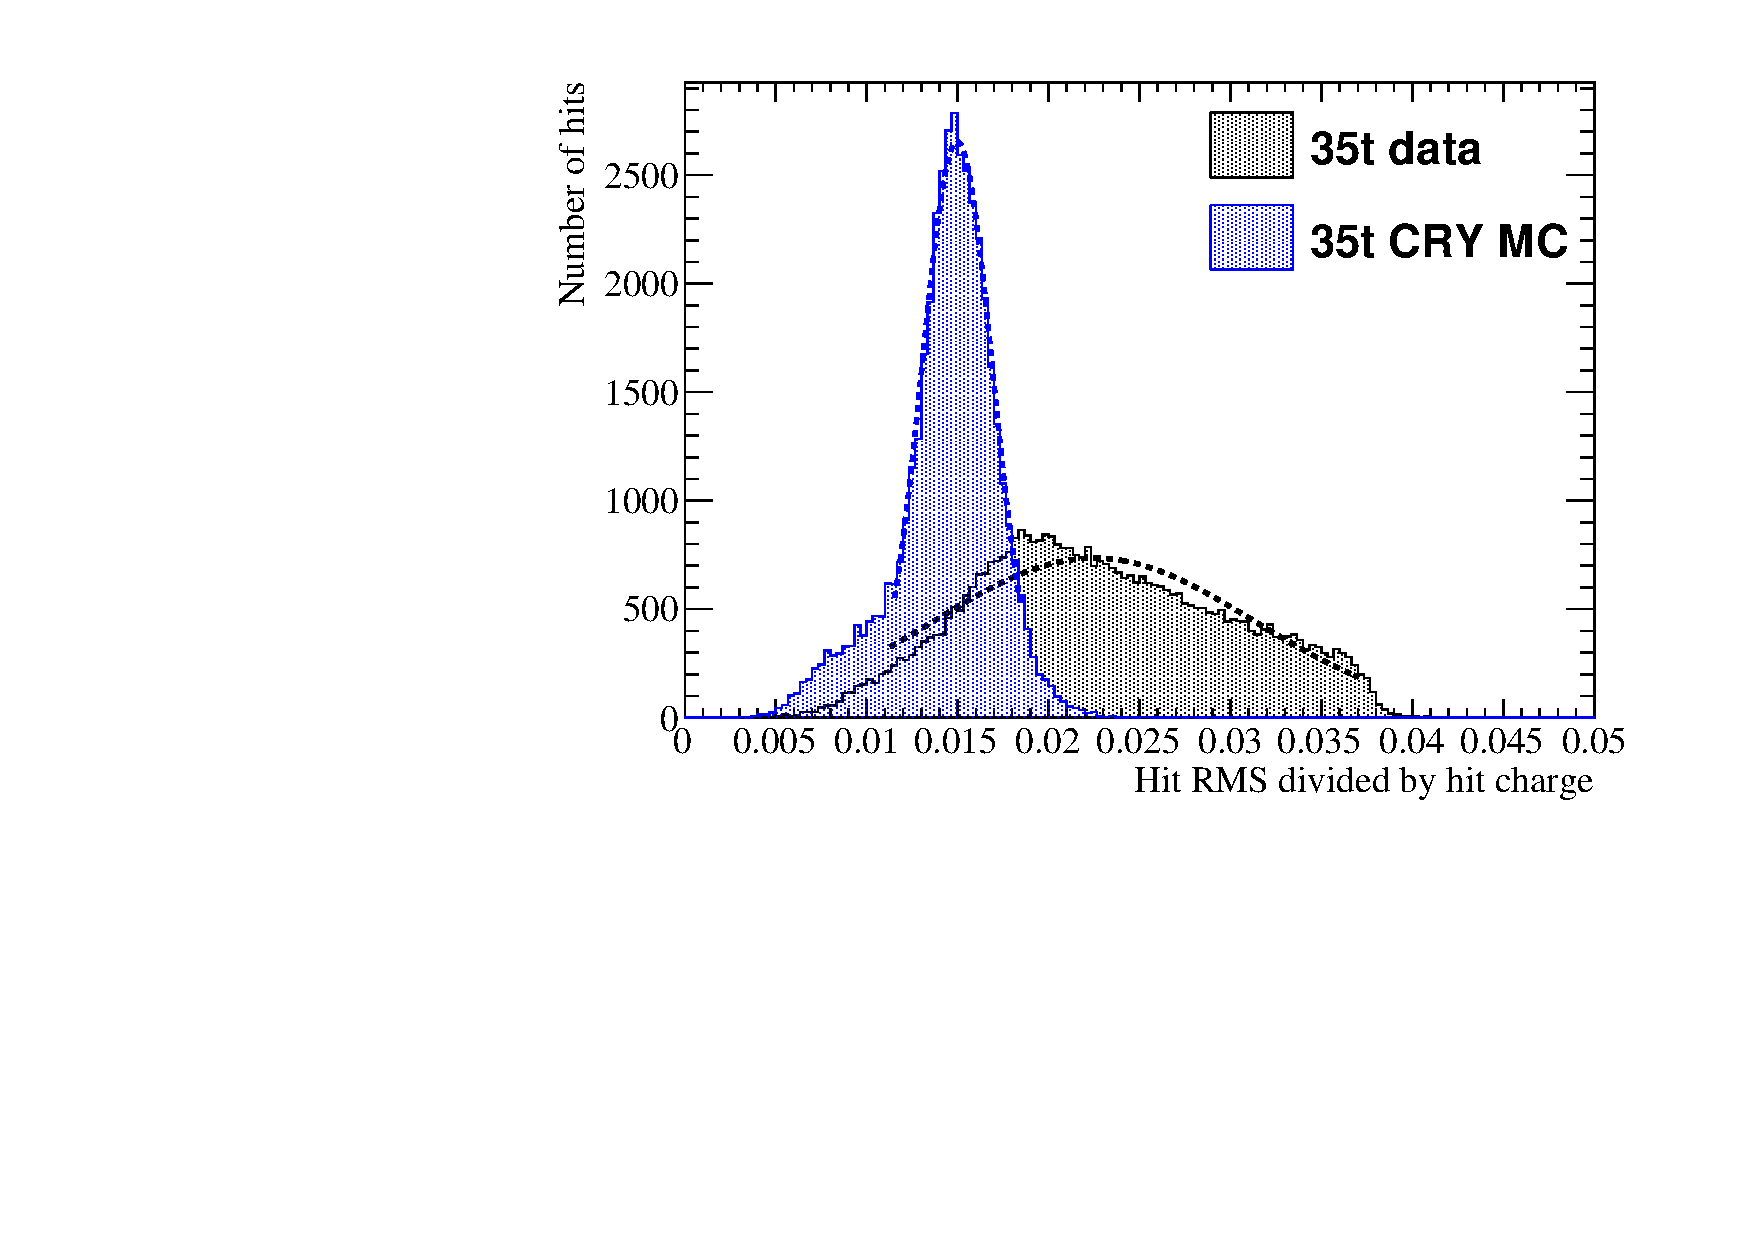
\includegraphics[width=\textwidth]{CombCan_2}
    \caption{The distribution of hit $RMS/Charge$ value for hits between $x =$ 20~cm and $x =$ 30~cm.}
  \end{subfigure}%
  \hspace{0.03\textwidth}%
  \begin{subfigure}{0.48\textwidth}
    \centering
    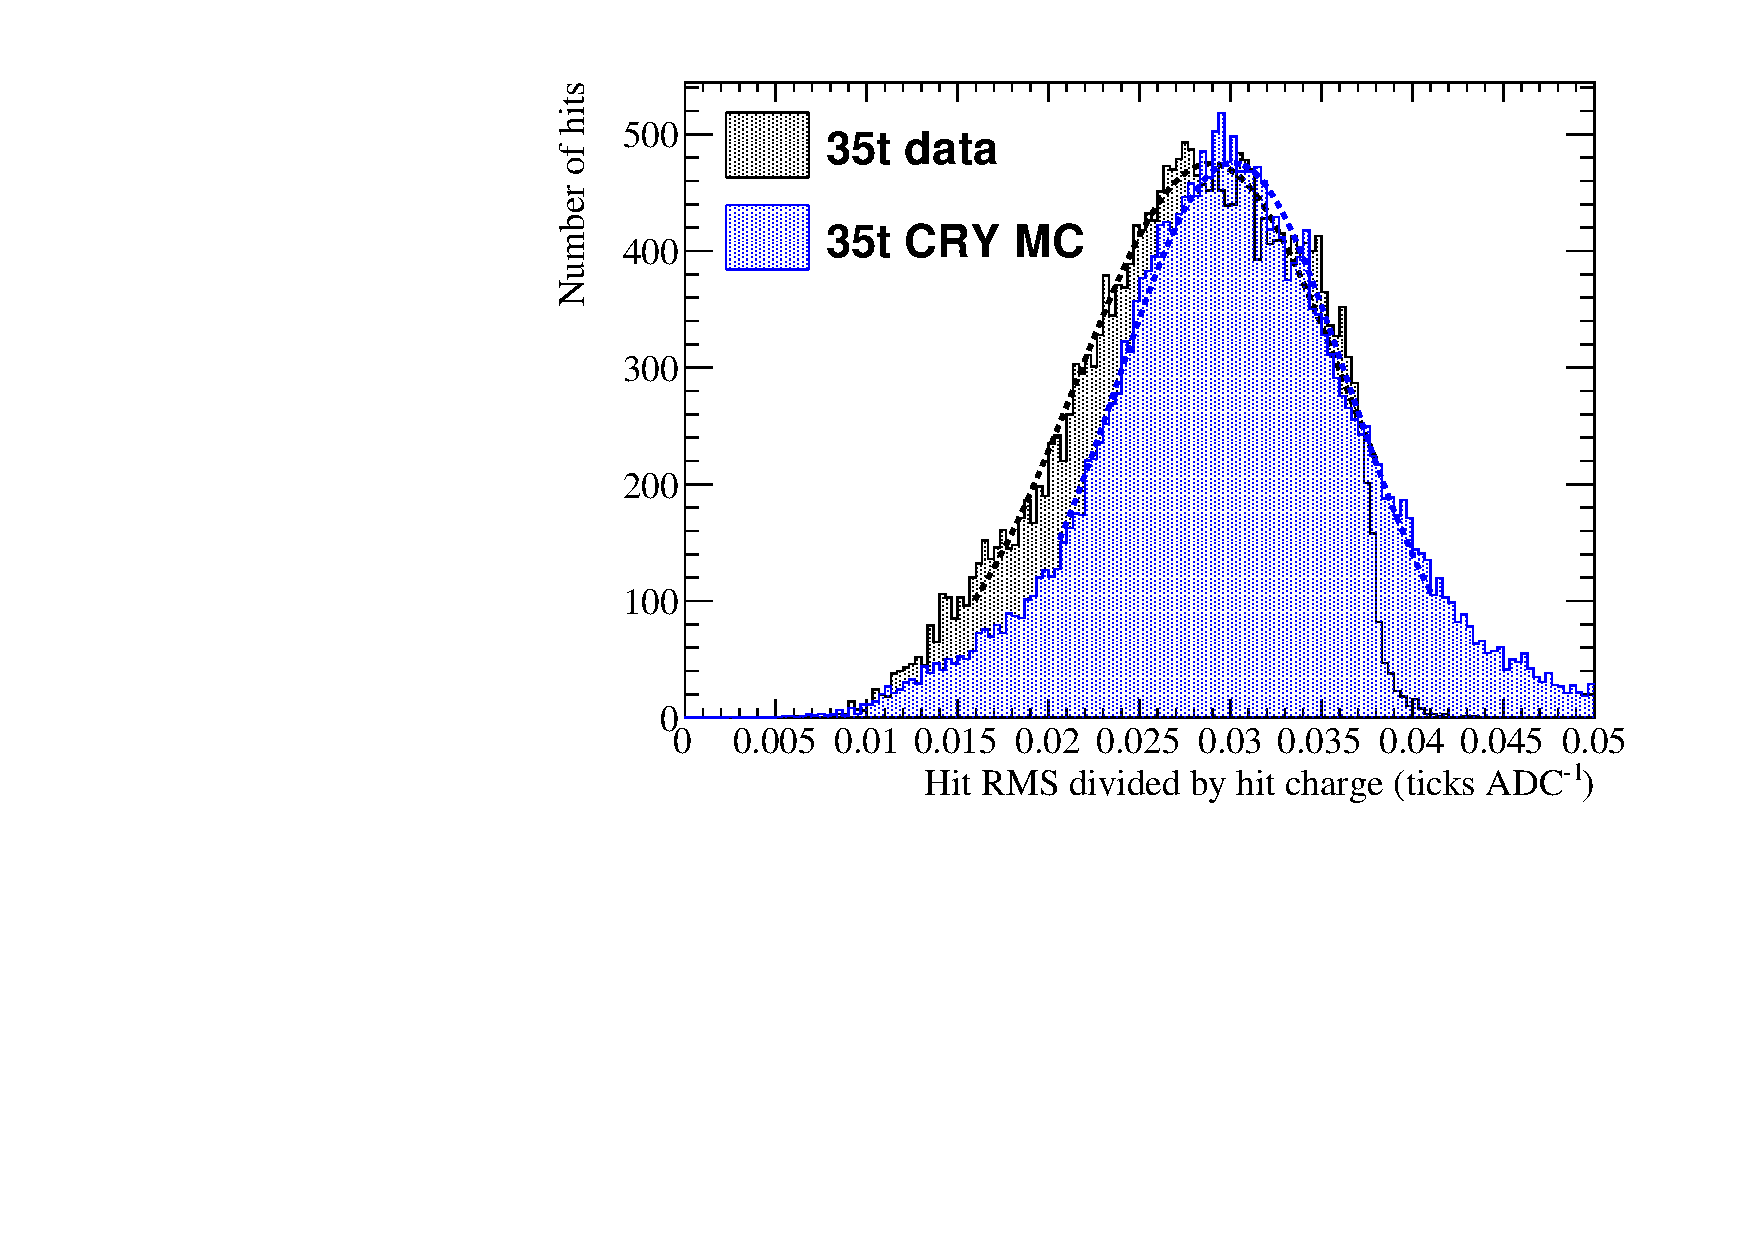
\includegraphics[width=\textwidth]{CombCan_3}
    \caption{The distribution of hit $RMS/Charge$ value for hits between $x =$ 140~cm and $x =$ 150~cm.}
    \label{fig:DiffMCHitFit_3}
  \end{subfigure}
  \caption[The distributions of hit $RMS$ and $RMS/Charge$ for tracks with a counter difference of 4 in the 35 ton dataset, and a low noise 35 ton detector]
          {The distributions of hit $RMS$ (top), and hit $RMS/Charge$ (bottom), for points between 20 and 30~cm from the APAs (left), and points between 140 and 150~cm from the APAs (right), for tracks associated with coincidences that have a counter differences of 4. The most probable values hit $RMS$ and hit $RMS/Charge$ are determined by fitting Gaussian functions around the peaks of the distributions. These fits are shown as dashed lines. The distributions for the 35 ton dataset are shown in black, whilst the distributions for the Monte Carlo simulation are shown in blue.}
          \label{fig:DiffMCHitFit}
\end{figure}

The most probable values of hit $RMS$ at increasing drift distance are shown in Figure~\ref{fig:DiffMCDataCompFit}, where the Monte Carlo simulation is again shown along with the values from the data. As was seen when considering the distributions at specific distances and counter differences, the most probable values of hit $RMS$ in the Monte Carlo simulation are systematically lower than in the data. This is attributed to the elevated noise level seen in the data, because, as seen in Figure~\ref{fig:DomsHitModel}, when a noise base-line is added to a signal, the width of the signal increases. Another difference between the Monte Carlo and the data, is that the gradient of the most probable values of hit $RMS$ in data is roughly half of that in the Monte Carlo. This could be due to an overestimation of the effect of longitudinal diffusion in the Monte Carlo sample, or, it could be due to the larger hit widths seen in the dataset at low drift distances, causing the effects of diffusion to be less apparent. Evidence for the latter can be seen in the stark differences between the figures in Figure~\ref{fig:DiffMCHitFit} at relatively short drift distances, compared to the similarities seen at large drift distances, where it appears that the Monte Carlo accurately simulates the distributions seen in the 35 ton dataset. \\

\begin{figure}
  \centering
  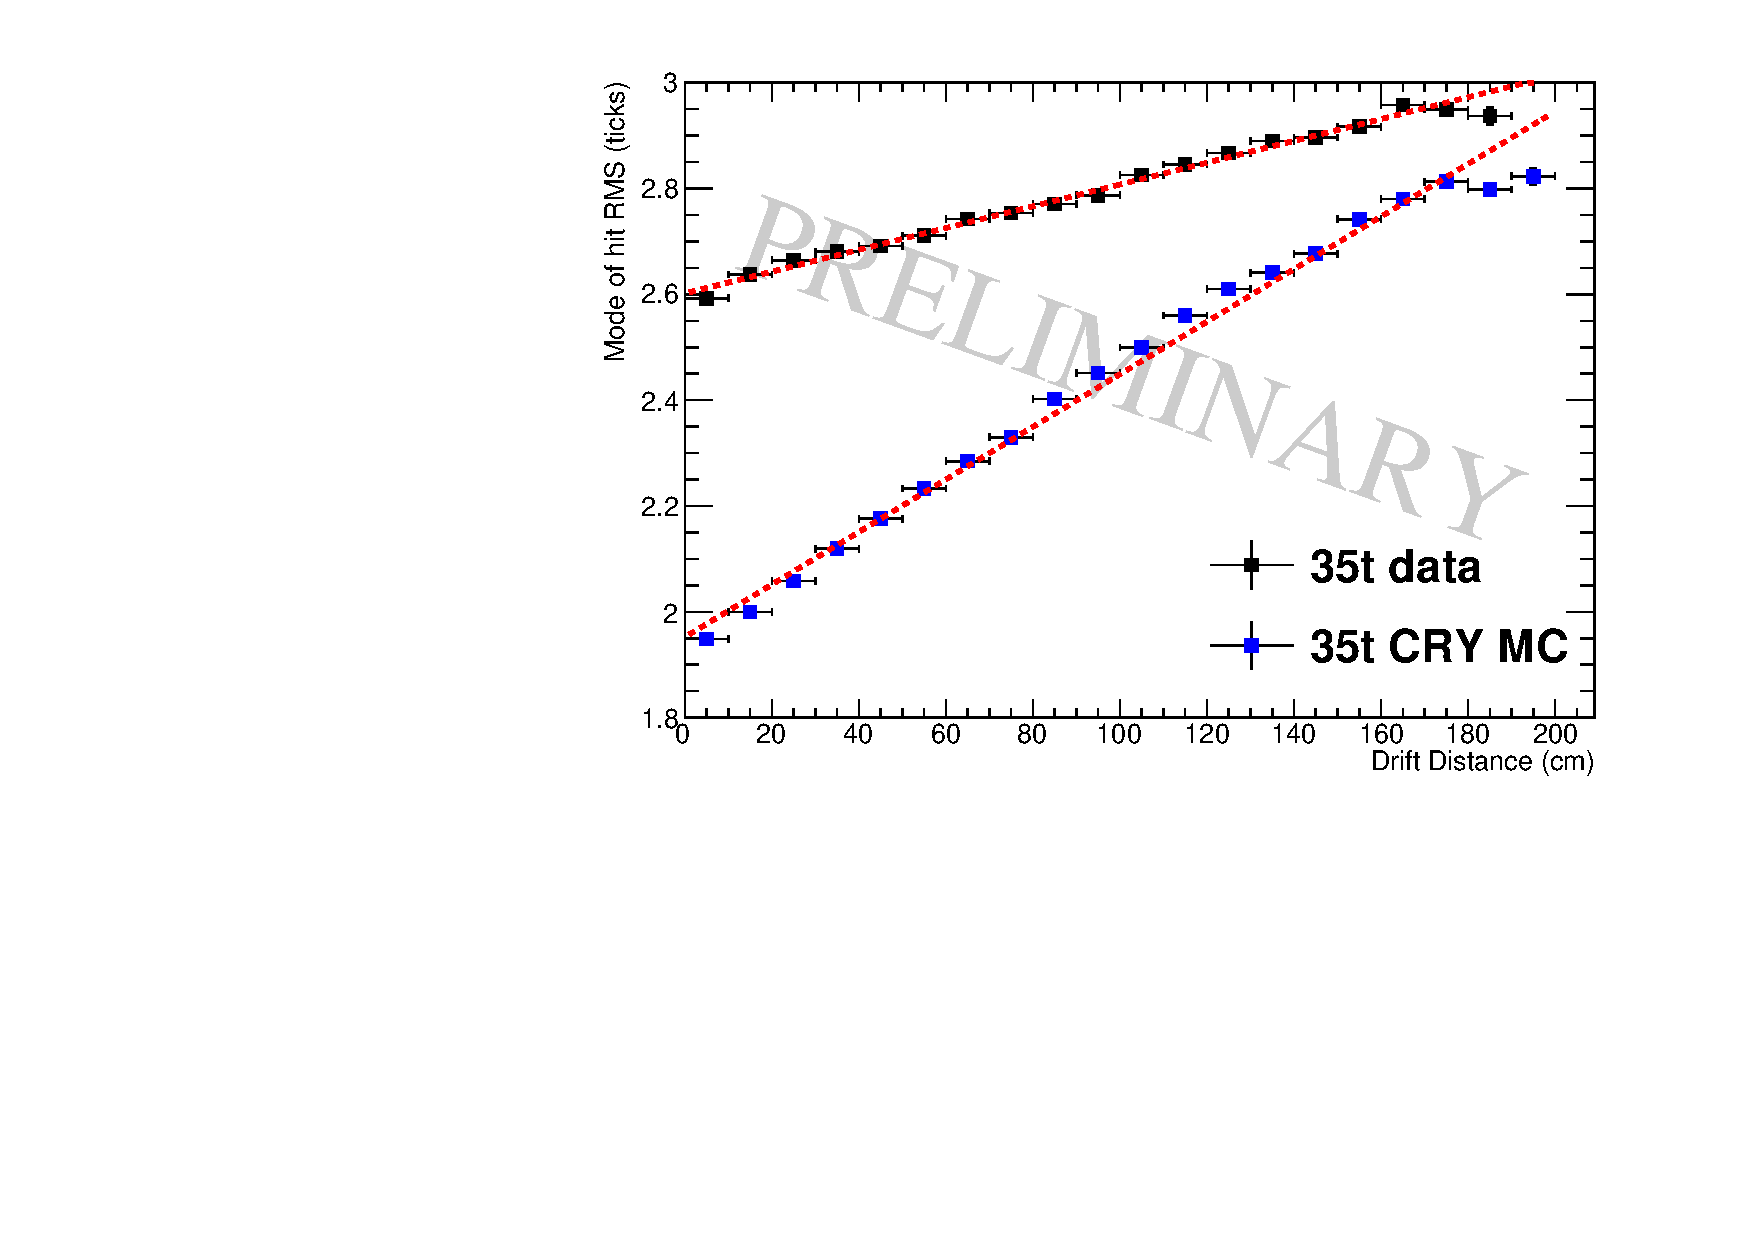
\includegraphics[width=0.6\textwidth]{CounterDiff4_Overlay}
  \caption[The drift distance dependence of diffusion in the 35 ton dataset and Monte Carlo for coincidences with a counter difference of 4]
          {The most probable values of hit $RMS$ as a function of drift distance, for tracks associated with a coincidence that had a counter difference of 4. The distribution for the 35 ton dataset is shown in black, whilst the distribution for the Monte Carlo simulation is shown in blue.}
  \label{fig:DiffMCDataCompFit}
\end{figure}

The most probable value of hit $RMS$ at a drift distance of 0~cm for a range of counter differences is shown in Figure~\ref{fig:DiffMCDataCompInt}. The change in MPV of hit $RMS$ can be seen to increase for both the Monte Carlo and 35 ton data samples, which again shows that the effects of diffusion can be seen to be track angle dependant. However, the way in which the MPV of hit $RMS$ increases is different in the two samples. The increased MPVs of hit $RMS$ seen in the 35 ton dataset, is again prescribed to the increase in hit width caused by the elevated noise level. \\

\begin{figure}
  \centering
  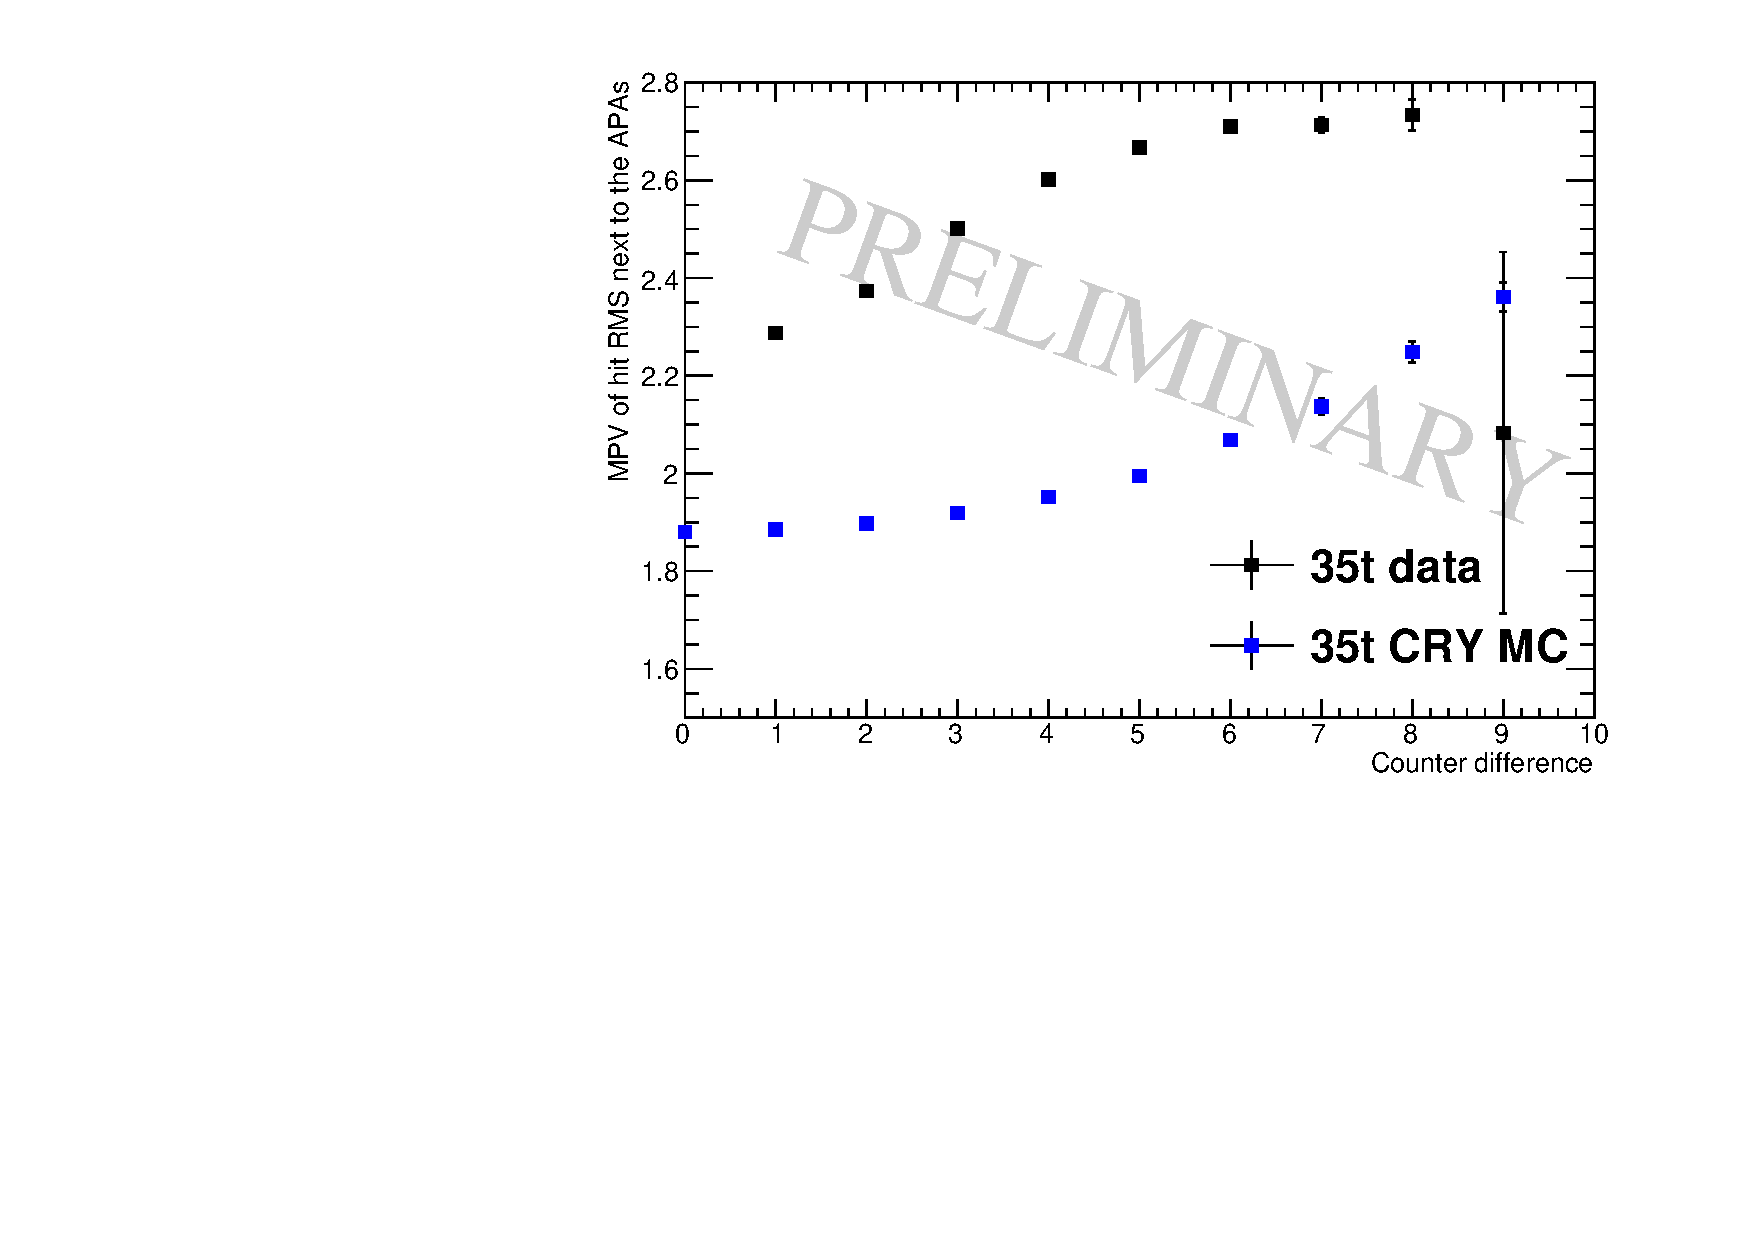
\includegraphics[width=0.6\textwidth]{InterceptCanvasOverlay}
  \caption[The angular dependence of diffusion in the 35 ton dataset and Monte Carlo for hits within 10~cm of the APAs]
          {The most probable values of hit $RMS$ within 10~cm of the APAs, as a function of the counter difference of the coincidence, that the track was associated with. The distribution for the 35 ton dataset is shown in black, whilst the distribution for the Monte Carlo simulation is shown in blue.}
  \label{fig:DiffMCDataCompInt}
\end{figure}

Upon calculating the fit metrics in the low-noise Monte Carlo dataset, it is then possible to use these to predict track interaction times. However, it is first necessary to calculate the normalised hit charge distributions, as was done for the 35 ton dataset. This is shown in Figure~\ref{fig:DiffOverlay_ChargeCut}. It can be seen that there are hits with lower values of hit $charge$ in the Monte Carlo sample, supporting the idea that there is a threshold effect in the 35 ton dataset. Importantly however, the aim of the cut to remove the tails of the hit $charge$ distributions can be seen to be successful in both the 35 ton dataset and Monte Carlo sample, as hits with large value of hit $charge$ are removed in both samples. The result of this will be that, the difference in predicted and reconstructed hit times, for a given track, will be centred on the interaction time of the track, as was presented in the discussion of Figure~\ref{fig:DiffData_ChargeCut}. The Monte Carlo hit times have been corrected using the time of the counter coincidence, as was the case for the 35 ton dataset. \\ 

\begin{figure}
  \centering
  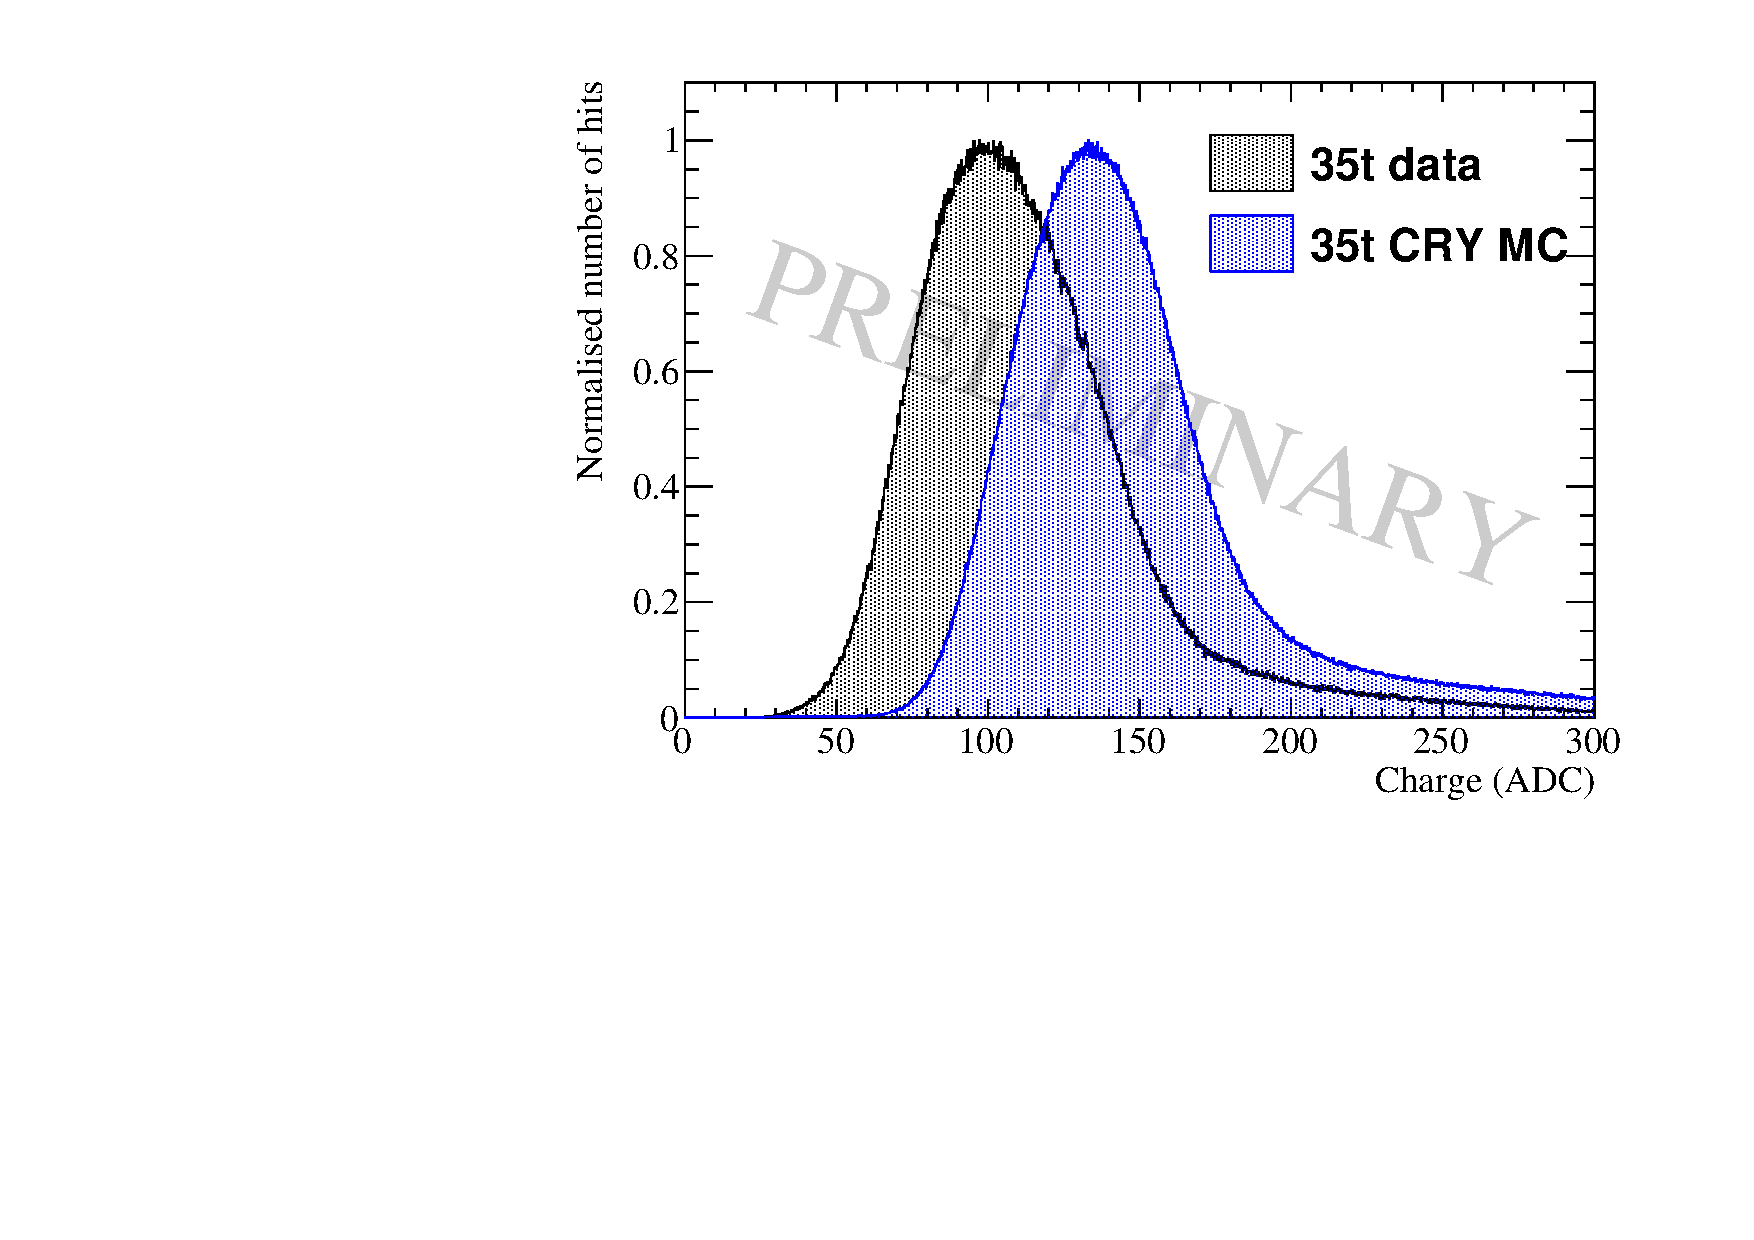
\includegraphics[width=0.6\textwidth]{ChargeCutOverlay}
  \caption[The distribution of normalised hit charge in the 35 ton dataset and a Monte Carlo sample]
          {The distribution of normalised hit charge, shown in units of ADC, in the 35 ton dataset and Monte Carlo sample. The number of hits with the most probable hit charge has been normalised to a value of 1. A cut on the normalised number of hits being greater than 0.25 is shown, the aim of this cut is to remove the tails of the hit charge distribution. The distribution for the 35 ton dataset is shown in black, whilst the distribution for the Monte Carlo simulation is shown in blue.}
  \label{fig:DiffOverlay_ChargeCut}
\end{figure}

Figure~\ref{fig:DiffOverlayAvDiff_RMS} compares how reliably the interaction time, and central $x$ position of a track, can be predicted using the effect that diffusion has on the hit $RMS$, in the 35 ton dataset and a low-noise Monte Carlo sample. As was the case when considering the 35 ton dataset, the average time difference ($x$ position) is calculated by taking the sum of individual hit differences for every hit in the track, and dividing this by the number of hits in the track. The accuracy in determining the interaction time in Monte Carlo (data) is found to be, 108~(240)~$\mu$s, where the distribution has a FWHM of 98~(281)~$\mu$s. When this is converted into the difference in central $x$ position of the track, the accuracy is found to be, 11.8~(27.7)~cm with a FWHM of 10.9~(32.1)~cm. \\

\begin{figure}
  \centering
  \begin{subfigure}{0.6\textwidth}
    \centering
    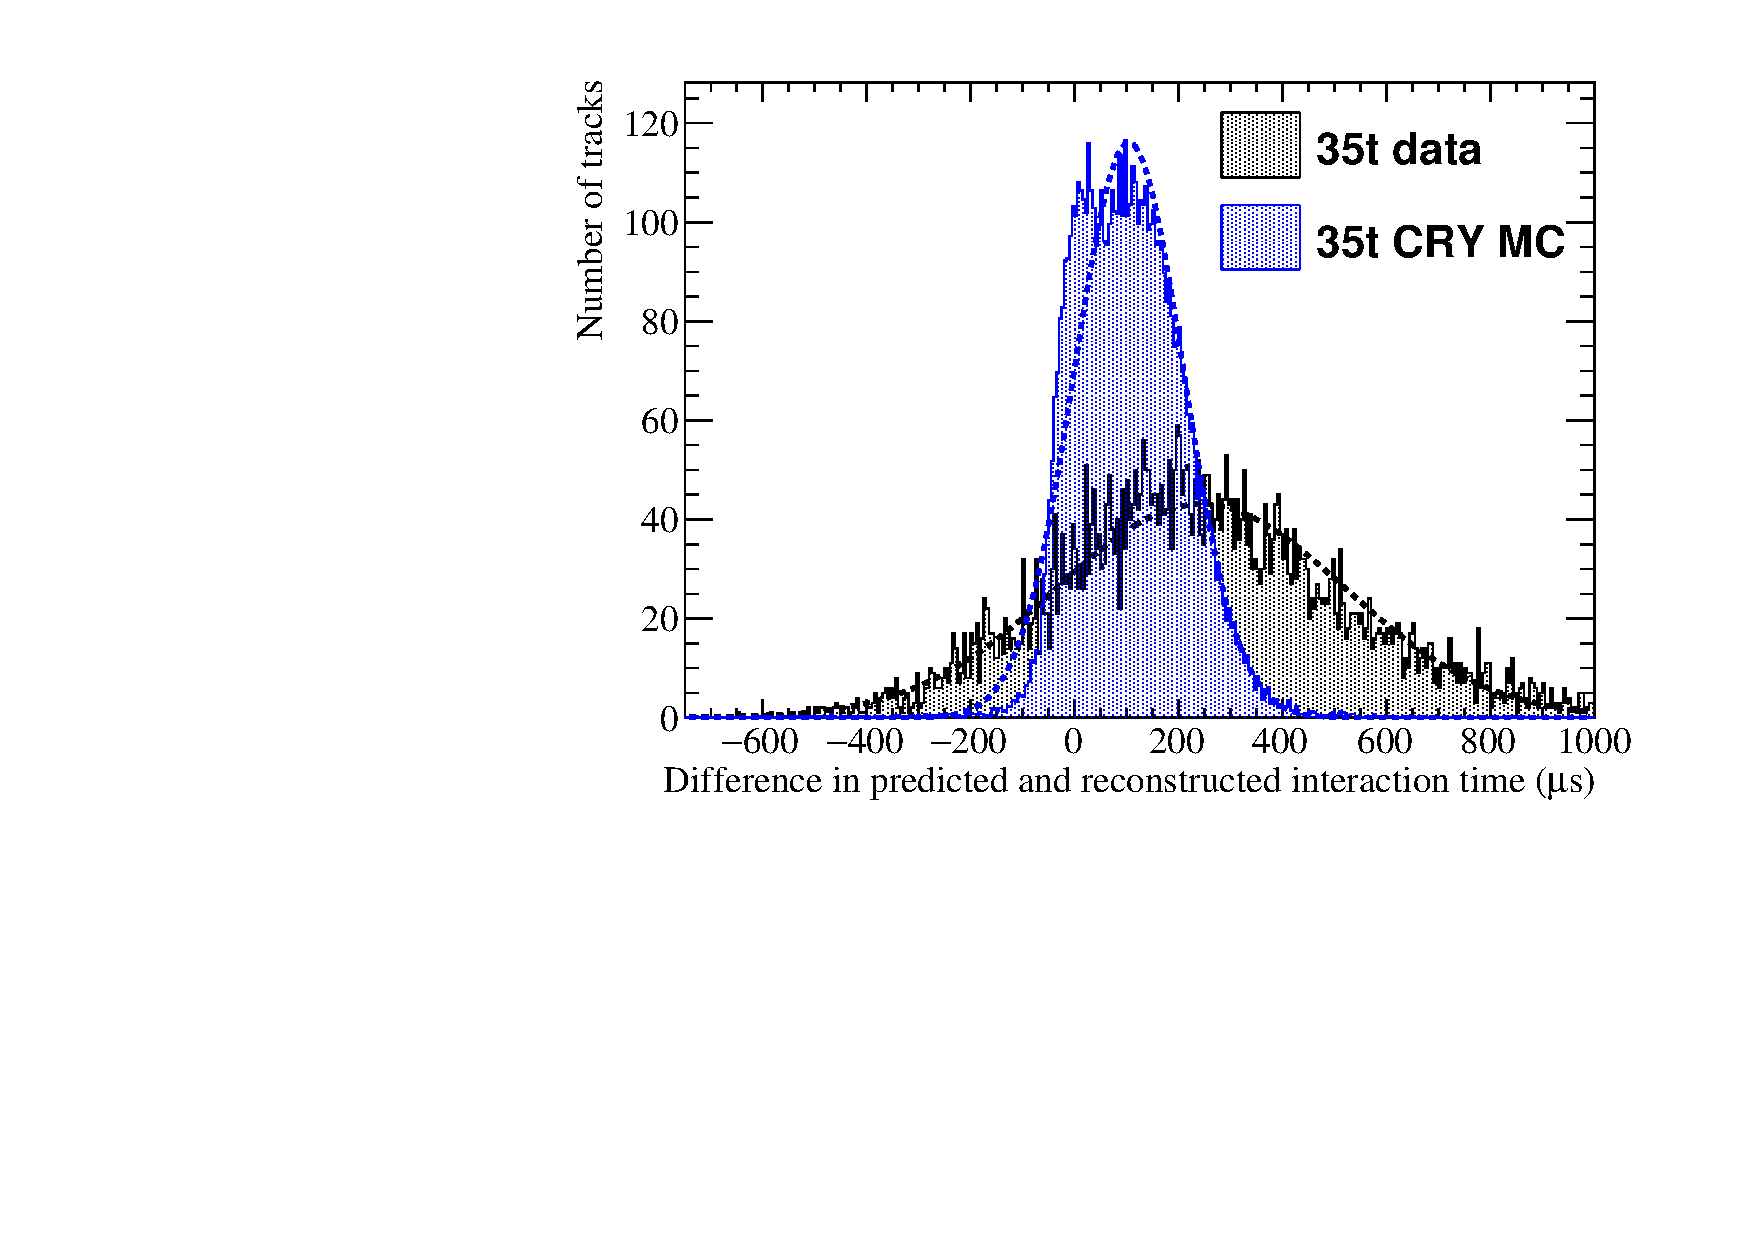
\includegraphics[width=\textwidth]{Overlay_AvTimeDiff_RMS}
    \caption{The average difference in interaction times using the hit $RMS$ metric.}
    \label{fig:DiffOverlayAvDiff_RMS_T}
  \end{subfigure}

  \begin{subfigure}{0.6\textwidth}
    \centering
    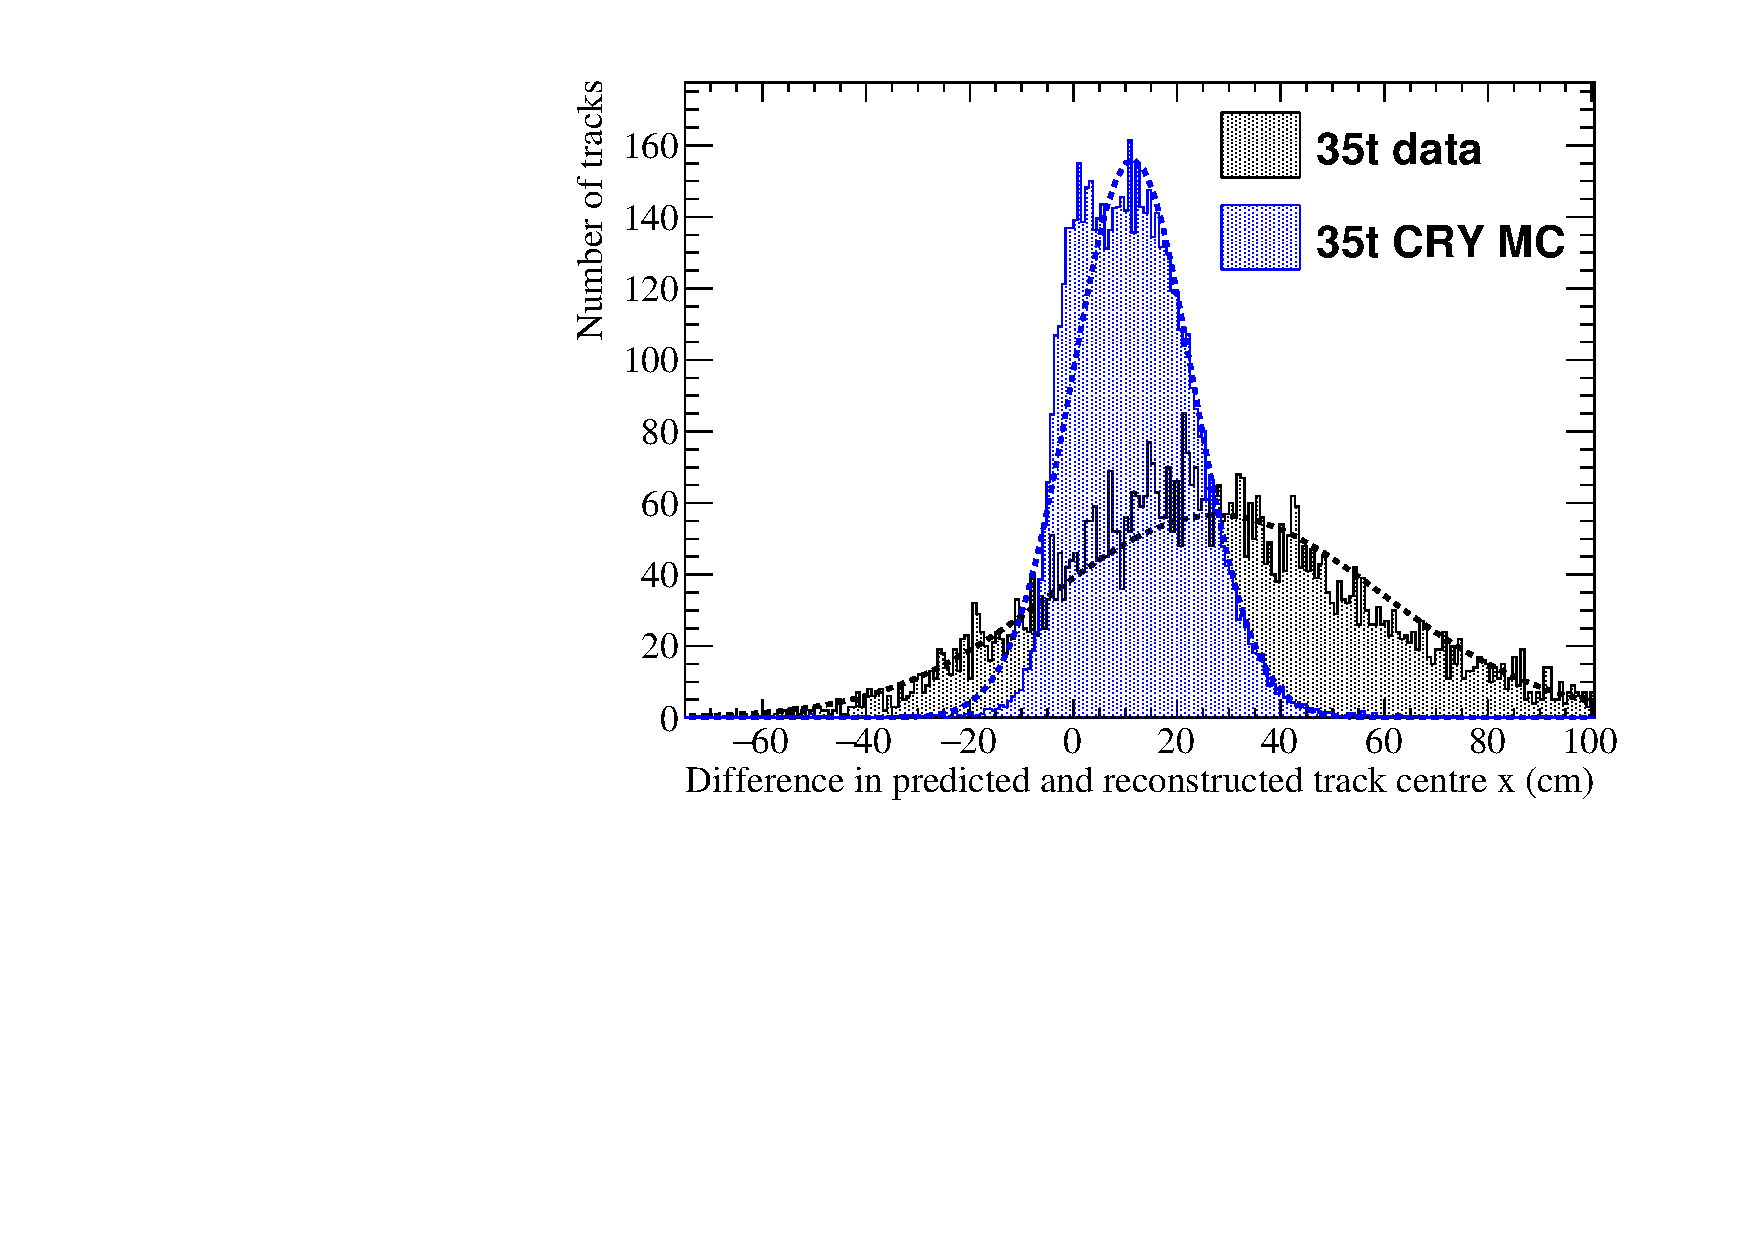
\includegraphics[width=\textwidth]{Overlay_AvXPosDiff_RMS}
    \caption{The average difference in the central $x$ position of a track using the hit $RMS$ metric.}
    \label{fig:DiffOverlayAvDiff_RMS_X}
  \end{subfigure}
  \caption[Comparing the accuracy of the hit $RMS$ method in the 35 ton dataset and a Monte Carlo simulation]
          {The accuracy of the hit $RMS$ method in the 35 ton dataset and a Monte Carlo simulation. Top: the accuracy to which interaction times can be determined in $\mu$s. Bottom: the accuracy to which the central $x$ position of a track can be determined. The average time difference ($x$ position) is calculated by taking the sum of individual hit differences for every hit in the track, and dividing this by the number of hits in the track. Gaussian functions are fitted to the distributions so that any offset in the predicted times or positions can be discerned. The distributions for the 35 ton dataset are shown in black, whilst the distributions for the Monte Carlo simulation are shown in blue}
  \label{fig:DiffOverlayAvDiff_RMS}
\end{figure}

Figure~\ref{fig:DiffOverlayAvDiff_RMS_Int} compares how reliably the interaction time, and central $x$ position, of a track can be predicted using the effect that diffusion has on the hit $RMS/Charge$, in the 35 ton dataset and a low-noise Monte Carlo sample. The accuracy in determining the interaction time in Monte Carlo (data) is found to be, 3~(171)~$\mu$s, where the distribution has a FWHM of 114~(210)~$\mu$s. When this is converted into the difference in central $x$ position of the track, the accuracy is found to be, 0.4~(18.5)~cm with a FWHM of 12.6~(23.0)~cm. \\

\begin{figure}
  \centering
  \begin{subfigure}{0.6\textwidth}
    \centering
    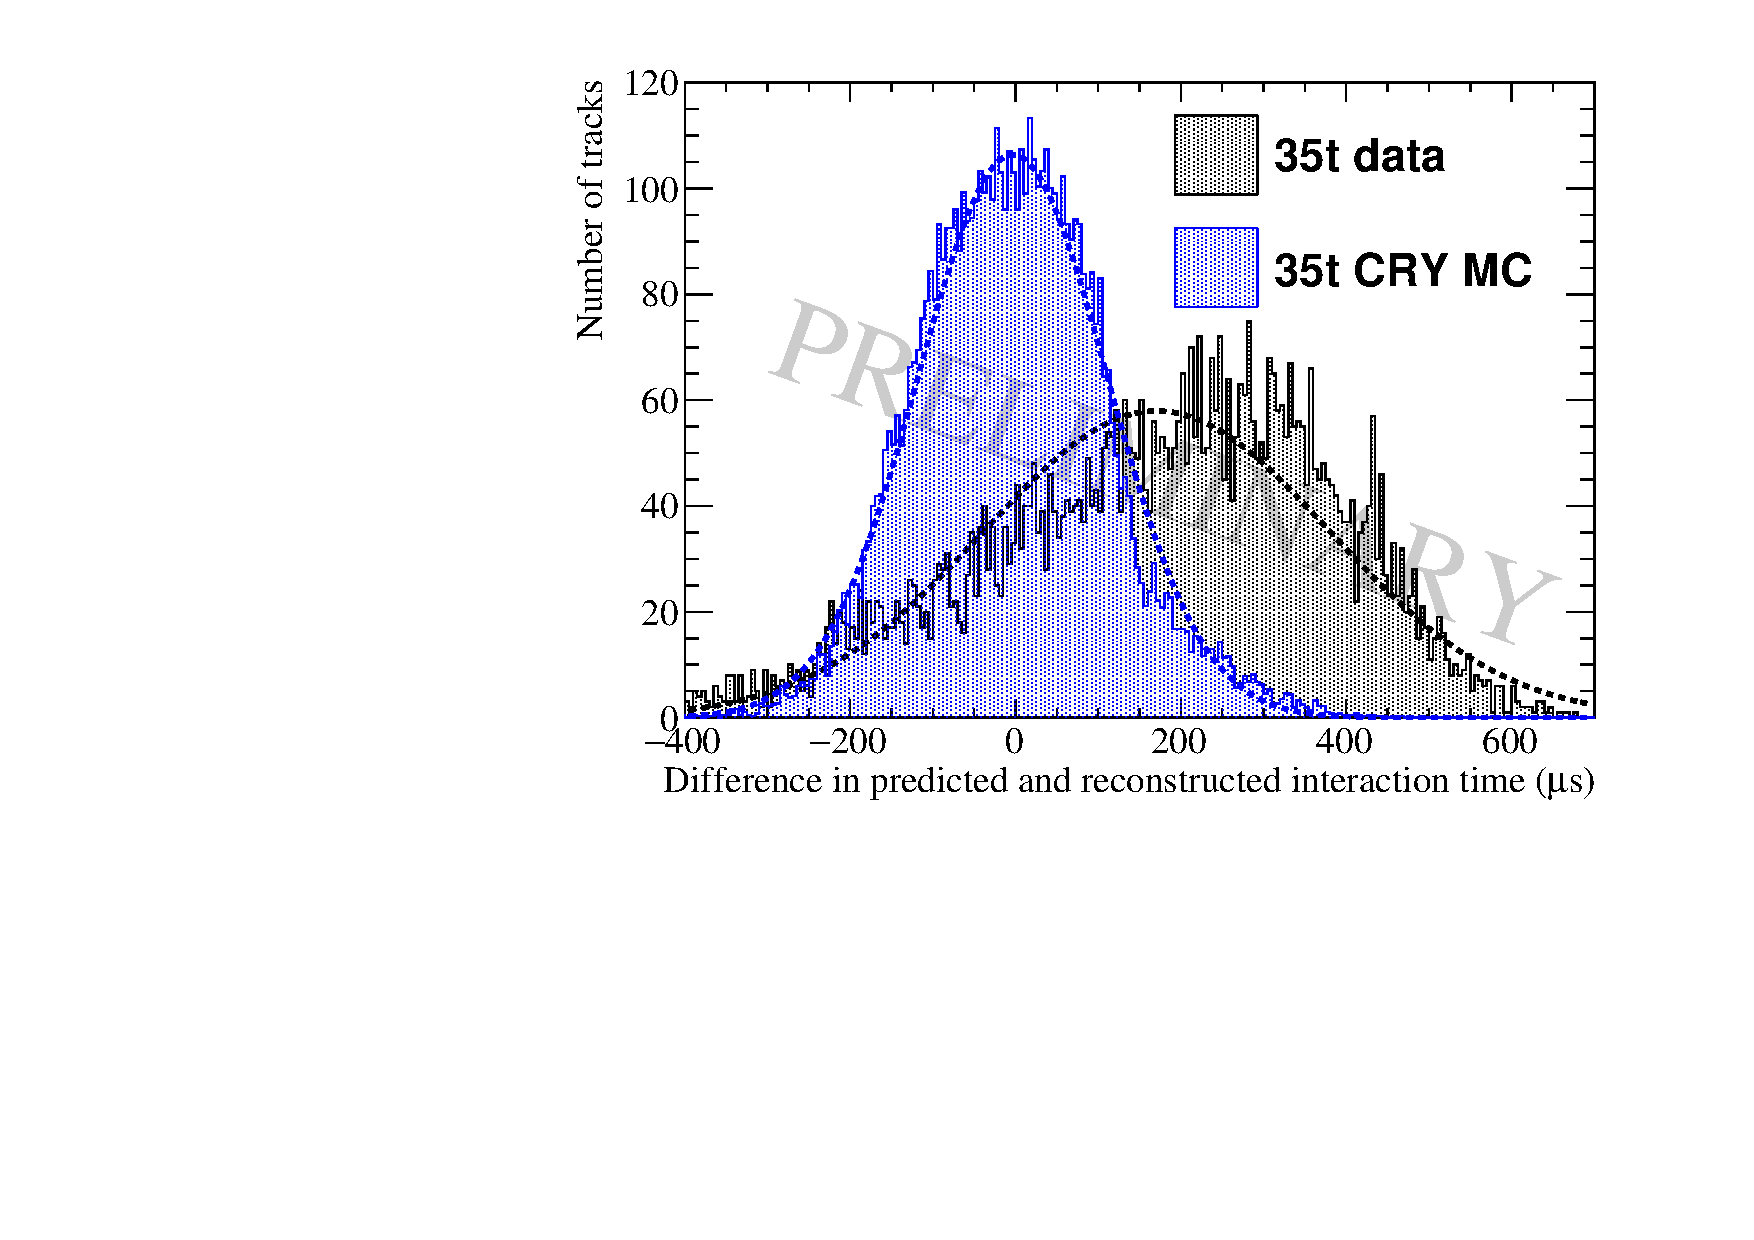
\includegraphics[width=\textwidth]{Overlay_AvTimeDiff_RMS_Int}
    \caption{The average difference in interaction times using the hit $RMS/Charge$ metric.}
    \label{fig:DiffOverlayAvDiff_RMS_Int_T}
  \end{subfigure}

  \begin{subfigure}{0.6\textwidth}
    \centering
    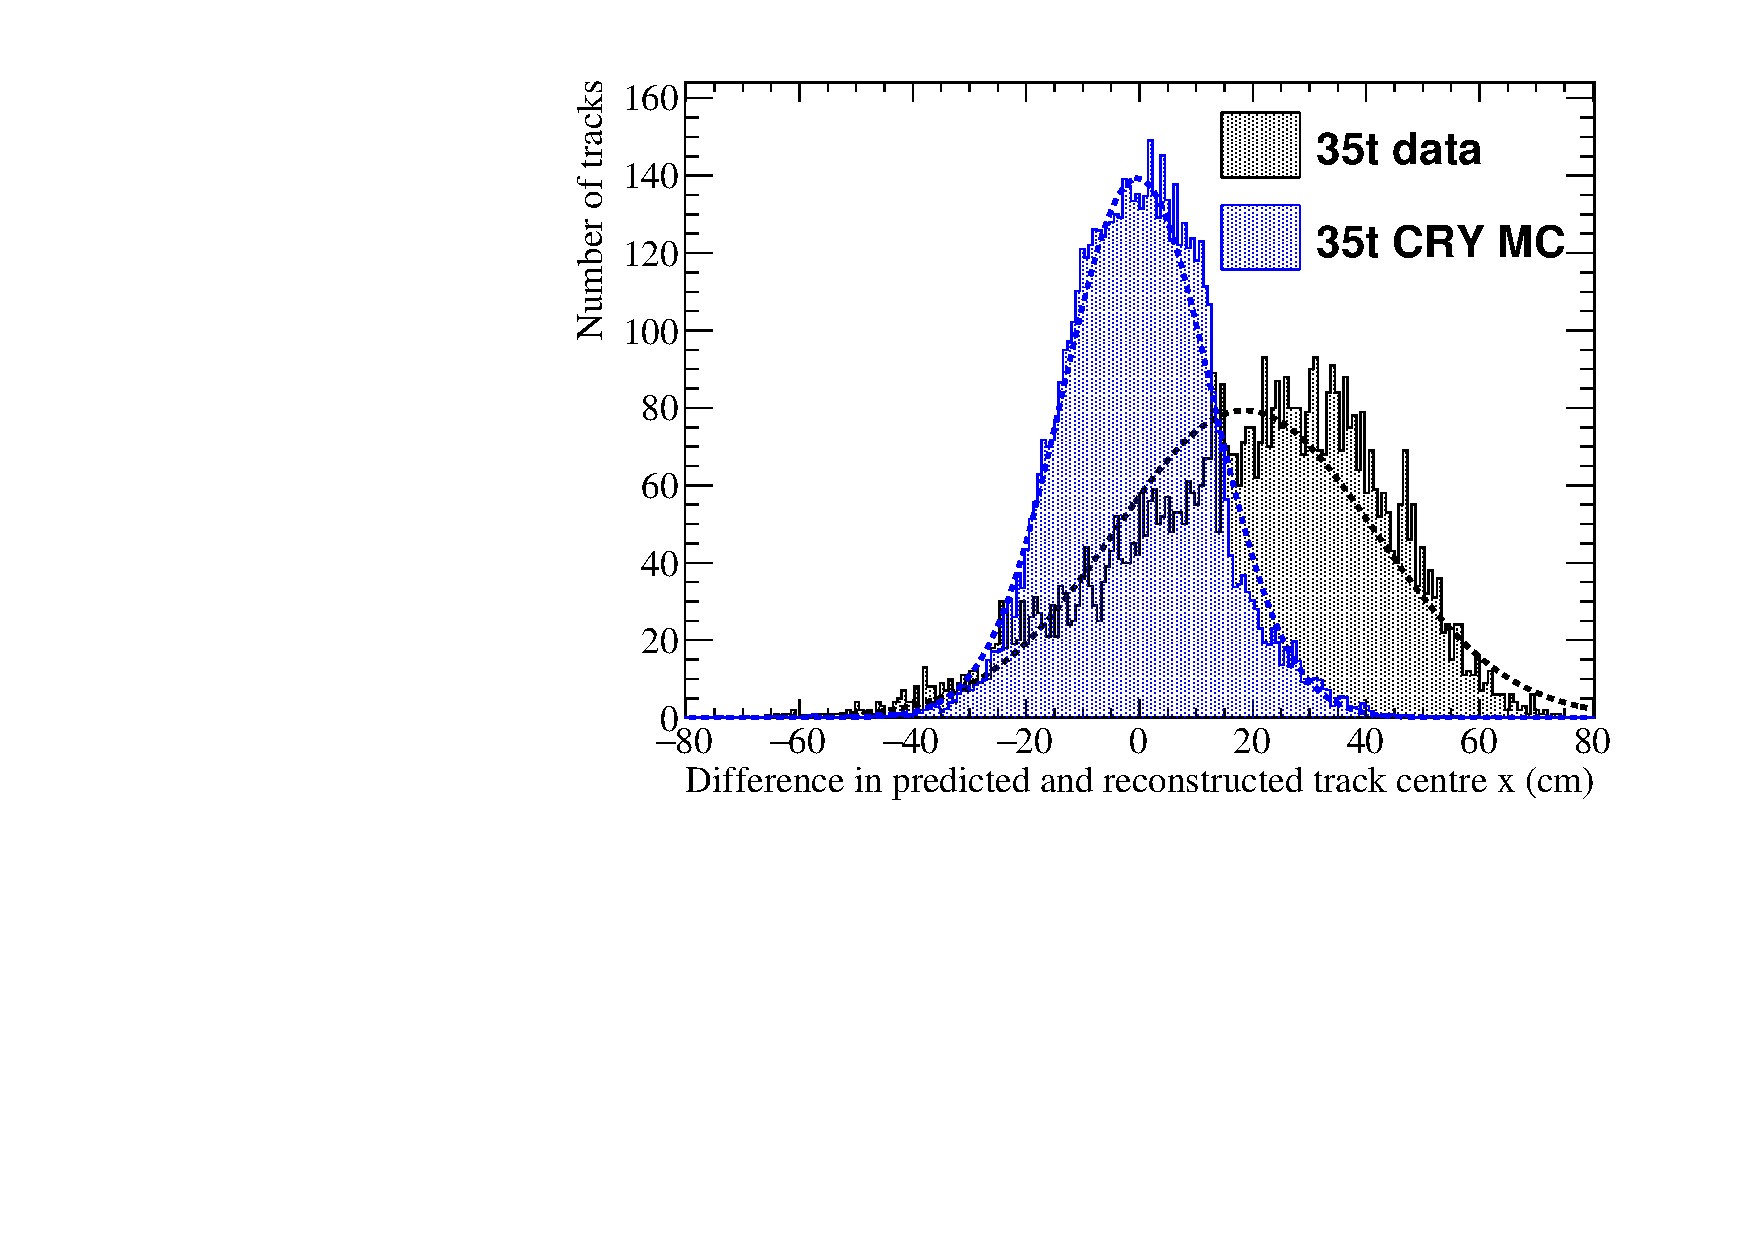
\includegraphics[width=\textwidth]{Overlay_AvXPosDiff_RMS_Int}
    \caption{The average difference in the central $x$ position of a track using the hit $RMS/Charge$ metric.}
    \label{fig:DiffOverlayAvDiff_RMS_Int_X}
  \end{subfigure}
  \caption[Comparing the accuracy of the hit $RMS$ method in the 35 ton dataset and a Monte Carlo simulation]
          {The accuracy of the hit $RMS/Charge$ method in the 35 ton dataset and a Monte Carlo simulation. Top: the accuracy to which interaction times can be determined in $\mu$s. Bottom: the accuracy to which the central $x$ position of a track can be determined. The average time difference ($x$ position) is calculated by taking the sum of individual hit differences for every hit in the track, and dividing this by the number of hits in the track. Gaussian functions are fitted to the distributions so that any offset in the predicted times or positions can be discerned. The distributions for the 35 ton dataset are shown in black, whilst the distributions for the Monte Carlo simulation are shown in blue}
  \label{fig:DiffOverlayAvDiff_RMS_Int}
\end{figure}

The hit $RMS/Charge$ metric appears to be able to more accurately predict interaction times, as was seen in when considering the only 35 ton dataset. This is again due to the ability to incorporate information about losses due to impurities, which increase with drift distance. Also, as expected from the previous figures, and the lower noise state in the Monte Carlo sample, it is seen that the interaction times predicted in the Monte Carlo sample more closely match the true interaction times, than was the case with the predictions made in the 35 ton dataset. An important feature to observe is that, as well as more accurately predicting the interaction times, the widths of the distributions in Monte Carlo are less than half of that in the data, particularly when using the hit $RMS$, as shown in Figure~\ref{fig:DiffOverlayAvDiff_RMS}. This means that the resolution with which tracks can be distinguished in the Monte Carlo sample is much better than in the 35 ton dataset, again this is attributed to the lower noise level in the Monte Carlo. \\

The calculation of interaction times is clearly much better in the low-noise Monte Carlo dataset, than in the 35 ton dataset. However, the distributions when using the hit $RMS$ are still not centred around 0, implying that there is a systematic error in the method, which has not been removed when considering a low-noise environment. The cut applied on the normalised hit $charge$ distribution was applied in order to remove the tails of the hit $RMS/Charge$ distribution, as seen in Figure~\ref{fig:DiffOverlay_ChargeCut}. Given that Figure~\ref{fig:DiffOverlayAvDiff_RMS_Int} shows that when using this metric, the predicted interaction times are centred on the reconstructed interaction times, this appears to have been successful. However, the analogous cut is not performed on the hit $RMS$ distribution, and so this could explain the decreased accuracy using this metric. \\

It is also possible that some $\delta$-rays have not been removed. This is because the only way to remove hits containing unseparated $\delta$-rays, is to look for the slight dip in the raw signal, which is associated with the $\delta$-ray moving away from the main track. This would be almost impossible in the 35 ton dataset given the oscillatory nature of the noise. Were a cut on hit $RMS$ to be applied, then these indistinguishable $\delta$-rays would likely be removed. This is because hits with $\delta$ rays would lie in the high value tails of the hit $RMS$ distribution, which the cut would remove. \\

The 35 ton dataset as a whole overestimates the interaction times though, and it is thought that this is due to elevated noise level. Justification for this assertion is discussed in Section~\ref{sec:DiffMCStudies} where the detector conditions of a simulated detector are varied. One of the detector conditions which is varied is the noise level in the detector. \\

%********************************** % Fifth.Third Section  *************************************
\subsection{Impact of changing detector properties using Monte Carlo samples} \label{sec:DiffMCStudies}
Much has been made of the difficulty that the noise level in the 35 ton dataset introduces, when performing reconstruction and analysis of the data. It is necessary to verify this claim, and so a sample of Monte Carlo events with increasing noise levels is produced, and analysed below. The noise level in the Monte Carlo samples is increased from the low-noise state used in the previous section, to a level more similar to that which is seen in the 35 ton dataset. If the claim that the noise level made reconstruction more difficult is correct, then the accuracy with which the interaction time can be determined should be seen to anti-correlate with the noise level of the simulated detector. In addition to varying noise levels, the electron lifetime, the electric field, and the constant of longitudinal diffusion are varied. All samples have used the same initial muons, this is done so that the only difference between the different samples are the detector conditions. Only one detector condition is varied at a time, so that the effect of each detector condition can be studied in isolation. As only one detector property is changed between samples, there is one sample that is consistent to all sample sets. This is when the RMS of the noise is 2.5~ADCs, the electron lifetime is 3~ms, the electric field is 500~V$\cdot$cm$^{-1}$, and the coefficient of longitudinal diffusion is 6.2$\times$10$^9$~cm$^2\cdot$ns$^{-1}$. When presenting the studies with changing detector conditions, only the accuracy with which the interaction time and central $x$ position of a track can be predicted, is shown here. A more robust collection of figures can be seen in Appendix~\ref{sec:DiffMCPlots}. \\

Figures~\ref{fig:DiffNoiseStudy_AvDiff_RMS} and~\ref{fig:DiffNoiseStudy_AvDiff_RMS_Int} show the effect that the increase in the noise level has on the accuracy to which the interaction time, and central $x$ position of a track, can be determined. \\

Figures~\ref{fig:DiffLifeStudy_AvDiff_RMS} and~\ref{fig:DiffLifeStudy_AvDiff_RMS_Int} show the effect that different electron lifetimes have on the accuracy to which the interaction time, and central $x$ position of a track, can be determined. \\

Figures~\ref{fig:DiffElecStudy_AvDiff_RMS} and~\ref{fig:DiffElecStudy_AvDiff_RMS_Int} show the effect that different electric fields have on the accuracy to which the interaction time, and central $x$ position of a track, can be determined. \\

Figures~\ref{fig:DiffLDiff_AvDiff_RMS} and~\ref{fig:DiffLDiff_AvDiff_RMS_Int} show the effect that different constants of longitudinal diffusion have on the accuracy to which the interaction time, and central $x$ position of a track, can be determined. \\

%%%%%%%% The noise simulation....
\begin{figure}
  \centering
  \begin{subfigure}{0.6\textwidth}
    \centering
    \includegraphics[width=\textwidth]{Canvas_AvDiff_T_RMS_NoiseLevel}
    \caption{The average difference in interaction times using the hit $RMS$ metric.}
    \label{fig:DiffNoiseStudy_AvDiffRMS_T}
  \end{subfigure}
  \begin{subfigure}{0.6\textwidth}
    \centering
    \includegraphics[width=\textwidth]{Canvas_AvDiff_X_RMS_NoiseLevel}
    \caption{The average difference in the central $x$ position of a track using the hit $RMS$ metric.}
    \label{fig:DiffNoiseStudy_AvDiffRMS_X}
  \end{subfigure}
  \caption[Comparing the accuracy of the hit $RMS$ method, as the electronic noise changes]
          {The accuracy of the hit $RMS$ method, for different electronic noise levels. Top: the accuracy to which interaction times can be determined in $\mu$s. Bottom: the accuracy to which the central $x$ position of a track can be determined. The average time difference ($x$ position) is calculated by taking the sum of individual hit differences for every hit in the track, and dividing this by the number of hits in the track. The 10 ADC RMS is not shown as the distribution is not contained within the graph.}
  \label{fig:DiffNoiseStudy_AvDiff_RMS}
\end{figure}

\begin{figure}
  \centering
  \begin{subfigure}{0.6\textwidth}
    \centering
    \includegraphics[width=\textwidth]{Canvas_AvDiff_T_RMS_Q_NoiseLevel}
    \caption{The average difference in interaction times using the hit $RMS/Charge$ metric.}
    \label{fig:DiffNoiseStudy_AvDiff_RMS_Int_T}
  \end{subfigure}
  \begin{subfigure}{0.6\textwidth}
    \centering
    \includegraphics[width=\textwidth]{Canvas_AvDiff_X_RMS_Q_NoiseLevel}
    \caption{The average difference in the central $x$ position of a track using the hit $RMS/Charge$ metric.}
    \label{fig:DiffNoiseStudy_AvDiff_RMS_Int_X}
  \end{subfigure}
  \caption[Comparing the accuracy of the hit $RMS$ method, as the electronic noise level changes]
          {The accuracy of the hit $RMS/Charge$ method, for different electronic noise levels. Top: the accuracy to which interaction times can be determined in $\mu$s. Bottom: the accuracy to which the central $x$ position of a track can be determined. The average time difference ($x$ position) is calculated by taking the sum of individual hit differences for every hit in the track, and dividing this by the number of hits in the track. The 10 ADC RMS is not shown as the distribution is not contained within the graph.}
  \label{fig:DiffNoiseStudy_AvDiff_RMS_Int}
\end{figure}

%%%%%%%% The Electron lifetime study
\begin{figure}
  \centering
  \begin{subfigure}{0.6\textwidth}
    \centering
    \includegraphics[width=\textwidth]{Canvas_AvDiff_T_RMS_ElecLifetime}
    \caption{The average difference in interaction times using the hit $RMS$ metric.}
    \label{fig:DiffLifeStudy_AvDiffRMS_T}
  \end{subfigure}
  \begin{subfigure}{0.6\textwidth}
    \centering
    \includegraphics[width=\textwidth]{Canvas_AvDiff_X_RMS_ElecLifetime}
    \caption{The average difference in the central $x$ position of a track using the hit $RMS$ metric.}
    \label{fig:DiffLifeStudy_AvDiffRMS_X}
  \end{subfigure}
  \caption[Comparing the accuracy of the hit $RMS$ method, as the electron lifetime changes]
          {The accuracy of the hit $RMS$ method, for different values of the electron lifetime. Top: the accuracy to which interaction times can be determined in $\mu$s. Bottom: the accuracy to which the central $x$ position of a track can be determined. The average time difference ($x$ position) is calculated by taking the sum of individual hit differences for every hit in the track, and dividing this by the number of hits in the track.}
  \label{fig:DiffLifeStudy_AvDiff_RMS}
\end{figure}

\begin{figure}
  \centering
  \begin{subfigure}{0.6\textwidth}
    \centering
    \includegraphics[width=\textwidth]{Canvas_AvDiff_T_RMS_Q_ElecLifetime}
    \caption{The average difference in interaction times using the hit $RMS/Charge$ metric.}
    \label{fig:DiffLifeStudy_AvDiff_RMS_Int_T}
  \end{subfigure}
  \begin{subfigure}{0.6\textwidth}
    \centering
    \includegraphics[width=\textwidth]{Canvas_AvDiff_X_RMS_Q_ElecLifetime}
    \caption{The average difference in the central $x$ position of a track using the hit $RMS/Charge$ metric.}
    \label{fig:DiffLifeStudy_AvDiff_RMS_Int_X}
  \end{subfigure}
  \caption[Comparing the accuracy of the hit $RMS$ method, as the electron lifetime changes]
          {The accuracy of the hit $RMS/Charge$ method, for different values of the electron lifetime. Top: the accuracy to which interaction times can be determined in $\mu$s. Bottom: the accuracy to which the central $x$ position of a track can be determined. The average time difference ($x$ position) is calculated by taking the sum of individual hit differences for every hit in the track, and dividing this by the number of hits in the track.}
  \label{fig:DiffLifeStudy_AvDiff_RMS_Int}
\end{figure}

%%%%%%%% The Electric field study
\begin{figure}
  \centering
  \begin{subfigure}{0.6\textwidth}
    \centering
    \includegraphics[width=\textwidth]{Canvas_AvDiff_T_RMS_ElecField}
    \caption{The average difference in interaction times using the hit $RMS$ metric.}
    \label{fig:DiffElecStudy_AvDiffRMS_T}
  \end{subfigure}
  \begin{subfigure}{0.6\textwidth}
    \centering
    \includegraphics[width=\textwidth]{Canvas_AvDiff_X_RMS_ElecField}
    \caption{The average difference in the central $x$ position of a track using the hit $RMS$ metric.}
    \label{fig:DiffElecStudy_AvDiffRMS_X}
  \end{subfigure}
  \caption[Comparing the accuracy of the hit $RMS$ method, as the electric field changes]
          {The accuracy of the hit $RMS$ method, for different values of the electric field. Top: the accuracy to which interaction times can be determined in $\mu$s. Bottom: the accuracy to which the central $x$ position of a track can be determined. The average time difference ($x$ position) is calculated by taking the sum of individual hit differences for every hit in the track, and dividing this by the number of hits in the track.}
  \label{fig:DiffElecStudy_AvDiff_RMS}
\end{figure}

\begin{figure}
  \centering
  \begin{subfigure}{0.6\textwidth}
    \centering
    \includegraphics[width=\textwidth]{Canvas_AvDiff_T_RMS_Q_ElecField}
    \caption{The average difference in interaction times using the hit $RMS/Charge$ metric.}
    \label{fig:DiffElecStudy_AvDiff_RMS_Int_T}
  \end{subfigure}
  \begin{subfigure}{0.6\textwidth}
    \centering
    \includegraphics[width=\textwidth]{Canvas_AvDiff_X_RMS_Q_ElecField}
    \caption{The average difference in the central $x$ position of a track using the hit $RMS/Charge$ metric.}
    \label{fig:DiffElecStudy_AvDiff_RMS_Int_X}
  \end{subfigure}
  \caption[Comparing the accuracy of the hit $RMS$ method, as the electric field changes]
          {The accuracy of the hit $RMS/Charge$ method, for different values of the electric field. Top: the accuracy to which interaction times can be determined in $\mu$s. Bottom: the accuracy to which the central $x$ position of a track can be determined. The average time difference ($x$ position) is calculated by taking the sum of individual hit differences for every hit in the track, and dividing this by the number of hits in the track.}
  \label{fig:DiffElecStudy_AvDiff_RMS_Int}
\end{figure}

%%%%%%%% The diffusion constant study

\begin{figure}
  \centering
  \begin{subfigure}{0.6\textwidth}
    \centering
    \includegraphics[width=\textwidth]{Canvas_AvDiff_T_RMS_Diffusion}
    \caption{The average difference in interaction times using the hit $RMS$ metric.}
    \label{fig:DiffLDiff_AvDiffRMS_T}
  \end{subfigure}
  \begin{subfigure}{0.6\textwidth}
    \centering
    \includegraphics[width=\textwidth]{Canvas_AvDiff_X_RMS_Diffusion}
    \caption{The average difference in the central $x$ position of a track using the hit $RMS$ metric.}
    \label{fig:DiffLDiff_AvDiffRMS_X}
  \end{subfigure}
  \caption[Comparing the accuracy of the hit $RMS$ method, as the constant of longitudinal diffusion changes]
          {The accuracy of the hit $RMS$ method, for different values of the constant of longitudinal diffusion. Top: the accuracy to which interaction times can be determined in $\mu$s. Bottom: the accuracy to which the central $x$ position of a track can be determined. The average time difference ($x$ position) is calculated by taking the sum of individual hit differences for every hit in the track, and dividing this by the number of hits in the track.}
  \label{fig:DiffLDiff_AvDiff_RMS}
\end{figure}

\begin{figure}
  \centering
  \begin{subfigure}{0.6\textwidth}
    \centering
    \includegraphics[width=\textwidth]{Canvas_AvDiff_T_RMS_Q_Diffusion}
    \caption{The average difference in interaction times using the hit $RMS/Charge$ metric.}
    \label{fig:DiffLDiff_AvDiff_RMS_Int_T}
  \end{subfigure}
  \begin{subfigure}{0.6\textwidth}
    \centering
    \includegraphics[width=\textwidth]{Canvas_AvDiff_X_RMS_Q_Diffusion}
    \caption{The average difference in the central $x$ position of a track using the hit $RMS/Charge$ metric.}
    \label{fig:DiffLDiff_AvDiff_RMS_Int_X}
  \end{subfigure}
  \caption[Comparing the accuracy of the hit $RMS$ method, as the constant of longitudinal diffusion changes]
          {The accuracy of the hit $RMS/Charge$ method, for different values of the constant of longitudinal diffusion. Top: the accuracy to which interaction times can be determined in $\mu$s. Bottom: the accuracy to which the central $x$ position of a track can be determined. The average time difference ($x$ position) is calculated by taking the sum of individual hit differences for every hit in the track, and dividing this by the number of hits in the track.}
  \label{fig:DiffLDiff_AvDiff_RMS_Int}
\end{figure}

%%%%%%%% The noise simulation....
Figures~\ref{fig:DiffNoiseStudy_AvDiff_RMS} and~\ref{fig:DiffNoiseStudy_AvDiff_RMS_Int} show the accuracy to which the interaction time, and central $x$ position of a track, can be determined using the effect that diffusion has on the hit $RMS$ and hit $RMS/Charge$, as the noise level in the detector changes. Figures~\ref{fig:DiffNoiseStudy_AvDiff_RMS} and~\ref{fig:DiffNoiseStudy_AvDiff_RMS_Int} both show that the accuracy of the fits decrease with increasing noise levels, but the decrease in accuracy is manifested in different ways. As discussed in Section~\ref{sec:AllTheNoise}, the 35 ton data had significant amounts of coherent noise which was not expected, and so this had not previously been simulated. As this level of coherent noise is not expected in future detectors, coherent noise has not been simulated in these increased noise level samples. Instead, the electronics noise, or ``thermal noise,'' has been varied. The lowest noise level was the design noise level for the 35 ton, and is the noise level that is used in the other figures in this section. This level of thermal noise is very minimal, and so only noise levels which are more than this have been simulated when the effect of the noise level in the detector is observed. This is because the $signal/noise$ ratio which one gets with such a low ADC RMS is large, and so a decrease in this noise level is unlikely to make a significant difference in the accuracy of the method. However, as can be seen in the 35 ton data, and the following plots, increasing the noise level has serious consequences. \\

No noise mitigation algorithms have been applied to the increased noise samples shown here. Instead, the threshold that the hit finder uses has been increased to the level that was necessary for a reasonable number of hits to be reconstructed. A reasonable number of hits simply means, not reconstructing such a large number of noise hits that they outweigh the number of true signals from tracks. The required hit threshold was determined by looking at the deconvoluted signal, and choosing a threshold which was above the majority of the noise signals. The hit thresholds used for each noise level are summarised below:
\begin{itemize}
\item Noise level of 2.5~ADC RMS - hit threshold of 6~ADC
\item Noise level of 5~ADC RMS - hit threshold of 10~ADC
\item Noise level of 7.5~ADC RMS - hit threshold of 15~ADC
\item Noise level of 10~ADC RMS - hit threshold of 20~ADC
\end{itemize}
This means that the main effect of increasing the noise level is to remove the low charge hits, as they will fall below the hit threshold, as it is increased to compensate for the increased noise level. \\

When considering Figure~\ref{fig:DiffNoiseStudy_AvDiff_RMS}, it can be seen that the accuracy to which interaction times can be determined rapidly decreases as the noise level increases. This is partly due to the fits used to make the prediction metrics not converging for counter differences of 1, 2, 3 and 4, as the MPV of hit $RMS$ is not seen to increase for increasing drift distances. For evidence of this, see the Figures in Appendix~\ref{sec:DiffMCPlots}. Though this is the extreme case, it can be seen that the validity of the hit $RMS$ for increasing drift distances becomes less predictable as the noise is increased. The result of this is a less accurate prediction metric, which leads to the large offsets and widths of the distributions that are shown in Figure~\ref{fig:DiffNoiseStudy_AvDiff_RMS}. This is particularly true for the sample which has a noise level of 10~ADC RMS, where the accuracy of the time determination is so bad that it is not contained on the plot. \\

The most striking feature of Figure~\ref{fig:DiffNoiseStudy_AvDiff_RMS_Int} is the decrease in statistics seen for the increasing noise levels. This shows the effect that increasing the noise level, and hence hit threshold has. This is because fewer tracks in total are reconstructed, and those that are reconstructed are less likely to meet the criteria about the number of collection hits required to make predictions. \\

%%%%%%%% The Electron lifetime study
Figure~\ref{fig:DiffLifeStudy_AvDiff_RMS} shows that with an electron lifetime of 1~ms, the hit $RMS$ metric is very inaccurate, this is likely due to hits which are a large distance away from the APAs being very difficult to reconstruct, because of the extremely poor lifetime. For this reason, the accuracy to which the hit $RMS$ metric predicts the interaction time improves as the electron lifetime increases, though this increase in small between the 3~ms, 5~ms and 8~ms samples. Figure~\ref{fig:DiffLifeStudy_AvDiff_RMS_Int} shows the opposite effect, the accuracy to which the interaction time can be determined decreases with increasing electron lifetime for the hit $RMS/Charge$ metric. This is shown by the widths of the distribution increasing as the electron lifetime increases. This happens because the decrease in hit charge is much greater when the electron lifetime is lower, and this dependence is the corner stone of this metric. The large decrease in hit charge for low electron lifetimes is why this metric performs so well for low electron lifetimes, and so the decrease in its accuracy is an unavoidable consequence of increasing electron lifetime. \\

%%%%%%%% The Electric field study
Figure~\ref{fig:DiffElecStudy_AvDiff_RMS} shows that the accuracy to which the interaction time can be predicted, increases with increasing electric field. This is shown by the introduction of an offset in the predicted interaction time for lower values of electric field strength. The opposite is shown in Figure~\ref{fig:DiffElecStudy_AvDiff_RMS_Int}, as the accuracy to which interaction time can be predicted does not see the introduction of an offset, and is slightly better for the samples with lower electric field strengths. However, when these interaction times are converted to the central $x$ position of a track, the accuracy is relatively unaffected by electric field strength. This is because the predicted central $x$ position are the same for all values of electric fields, and are peaked at the true central $x$ position for both samples. However, there is a large sample of tracks in Figure~\ref{fig:DiffElecStudy_AvDiff_RMS} with an offset of about 10~cm, which makes the distribution of the average difference in predicted central $x$ positions to not be Gaussian. The presence of this offset in both samples shows that the hit $RMS$ and hit $RMS/Charge$ metrics are both relatively unaffected by the electric field strength. \\

%%%%%%%% The diffusion constant study
As would be expected, both Figures~\ref{fig:DiffLDiff_AvDiff_RMS} and~\ref{fig:DiffLDiff_AvDiff_RMS_Int} show that the accuracy to which the interaction time and central $x$ position can be predicted are highly dependant on the longitudinal diffusion constant. This is seen by the distributions becoming much narrower, and more closely centred around the true interaction time, or central $x$ position, as the constant of longitudinal diffusion increases. It is interesting to note that the extremely poor resolution seen in Figure~\ref{fig:DiffLDiff_AvDiff_RMS} when there is no longitudinal diffusion, is not present in Figure~\ref{fig:DiffLDiff_AvDiff_RMS_Int}. It is thought that this is due to the effect of charge attenuation, which will still occur because of the finite electron lifetime. 

%********************************** % Fifth.Fourth Section  *************************************
\subsection{The limitations of and future improvements to the method of interaction time determination using diffusion} \label{sec:DiffLimitations}
The comparison of the 35 ton data and Monte Carlo samples, as well as the Monte Carlo samples with differing detector conditions, show that there is potential in the ability to determine interaction times using the effects of diffusion. However, there are still some issues which need to be overcome, some of these are briefly discussed below. \\

Many of the figures shown still have slight offsets even though the tails of the hit charge distributions have been removed. However, these offsets are generally confined to detector conditions which would not be considered optimal, such as very low electron lifetimes (1~ms) or high detector noise. The latter is seen to be the case when considering the 35 ton dataset, where the high noise scale can be seen to affect the accuracy to which the interaction time, and central $x$ position, can be determined. A potential solution to reduce these offsets, and also to reduce the width of the distributions, is to perform the interaction time determination twice. The result of the first run, which is what is shown in this thesis, would then be used to select only hits which lie within the expected regions of hit $RMS$ and hit $RMS/Charge$. This would be possible as the initial interaction time determination could be used to work out the rough $x$ positions of hits, and then only hits which lie within a given region of the MPV would be used to determine the interaction time from the second pass. When performing the second pass of interaction time determination, the size of this region would be a user defined parameter, but would need to be small enough so as to exclude the beginnings of the tails of the hit $RMS$, and hit $RMS/Charge$, distributions. \\

%All of the figures shown that had the difference in predicted and reconstructed interaction times were not centered around 0~$\mu$s and also had large FWHMs. It is thought that this is due to interpreting distributions which are not Gaussian as Gaussian functions, such as Figure~\ref{fig:DiffMCHitFit}. This means that when the MPVs are calculated using only the values around the peaks, there are large tails at both high and low values which are not counted. As the hits which make up these tails are still used to predict the interaction times they will introduce the observed offsets as the times which they would predict will be far from that which the MPV would predict. The result of this is that the assumption made earlier, that over a large number of hits the average predicted interaction time will be correct, could no longer hold. A potential solution to remedy this, is to refine the selection of hits that are used to predict the interaction time to exclude the extreme values of these tails. However, to do this accurately would require some knowledge of the hit location, as the MPV of hit $RMS$ can change significantly over the drift length of the detector. This is shown in Figure~\ref{fig:DiffMCDataCompFit}, where the MPV of hit $RMS$ in Monte Carlo changes from roughly 1.9~ticks near the APAs to roughly 2.8~ticks 200~cm away from the APAs. Looking at the top plots in Figure~\ref{fig:DiffMCHitFit}, this range encompasses the entire distrbibution of Monte Carlo hit $RMS$ values, including the tail of hit $RMS$ above 2.3~ticks which we would like to remove. Another solution to improving the accuracy of the predicted interaction time could be to weight the predicted interaction times from each hit in some way which better represents the distribution of hit $RMS$ and hit $RMS/Charge$ seen in Figure~\ref{fig:DiffMCHitFit}. \\

An important improvement to the method would be to expand it to include the induction plane wires, as this will greatly increase both the number of wires which can be used, and the range of track angles whose interaction times can be predicted. The angular range of the method would increase, since, when using only collection plane wires, it is impossible to reconstruct enough hits for nearly vertical muons, as very few wires would be hit. This was discussed in Section~\ref{sec:SimRecoEffic}. This was not attempted here, as the electronics noise in the 35 ton data was too large to able to reliably reconstruct hits on the induction planes, without reconstructing many noise hits. This meant that the hit threshold on the induction planes was very high. \\
